%&preformat-disser
\RequirePackage[l2tabu,orthodox]{nag} % Раскомментировав, можно в логе получать рекомендации относительно правильного использования пакетов и предупреждения об устаревших и нерекомендуемых пакетах
% Формат А4, 14pt (ГОСТ Р 7.0.11-2011, 5.3.6)
\documentclass[a4paper,14pt,oneside,openany]{memoir}
\usepackage{import}

%%%%%%%%%%%%%%%%%%%%%%%%%%%%%%%%%%%%%%%%%%%%%%%%%%%%%%%
%%%% Файл упрощённых настроек шаблона автореферата %%%%
%%%%%%%%%%%%%%%%%%%%%%%%%%%%%%%%%%%%%%%%%%%%%%%%%%%%%%%

%%% Инициализирование переменных, не трогать!  %%%
\newcounter{showperssign}
\newcounter{showsecrsign}
\newcounter{showopplead}
%%%%%%%%%%%%%%%%%%%%%%%%%%%%%%%%%%%%%%%%%%%%%%%%%%%%%%%

%%% Список публикаций %%%
\makeatletter
\@ifundefined{c@usefootcite}{
  \newcounter{usefootcite}
  \setcounter{usefootcite}{0} % 0 --- два (или более) списка литературы;
                              % 1 --- список публикаций автора + цитирование
                              %       других работ в сносках
}{}
\makeatother

\makeatletter
\@ifundefined{c@bibgrouped}{
  \newcounter{bibgrouped}
  \setcounter{bibgrouped}{0}  % 0 --- единый список работ автора;
                              % 1 --- сгруппированные работы автора
}{}
\makeatother

%%% Область упрощённого управления оформлением %%%

%% Управление зазором между подрисуночной подписью и основным текстом %%
\setlength{\belowcaptionskip}{10pt plus 20pt minus 2pt}


%% Подпись таблиц %%

% смещение строк подписи после первой
\newcommand{\tabindent}{0cm}

% тип форматирования таблицы
% plain --- название и текст в одной строке
% split --- название и текст в разных строках
\newcommand{\tabformat}{plain}

%%% настройки форматирования таблицы `plain'

% выравнивание по центру подписи, состоящей из одной строки
% true  --- выравнивать
% false --- не выравнивать
\newcommand{\tabsinglecenter}{false}

% выравнивание подписи таблиц
% justified   --- выравнивать как обычный текст
% centering   --- выравнивать по центру
% centerlast  --- выравнивать по центру только последнюю строку
% centerfirst --- выравнивать по центру только первую строку
% raggedleft  --- выравнивать по правому краю
% raggedright --- выравнивать по левому краю
\newcommand{\tabjust}{justified}

% Разделитель записи «Таблица #» и названия таблицы
\newcommand{\tablabelsep}{~\cyrdash\ }

%%% настройки форматирования таблицы `split'

% положение названия таблицы
% \centering   --- выравнивать по центру
% \raggedleft  --- выравнивать по правому краю
% \raggedright --- выравнивать по левому краю
\newcommand{\splitformatlabel}{\raggedleft}

% положение текста подписи
% \centering   --- выравнивать по центру
% \raggedleft  --- выравнивать по правому краю
% \raggedright --- выравнивать по левому краю
\newcommand{\splitformattext}{\raggedright}

%% Подпись рисунков %%
%Разделитель записи «Рисунок #» и названия рисунка
\newcommand{\figlabelsep}{~\cyrdash\ }  % (ГОСТ 2.105, 4.3.1)
                                        % "--- здесь не работает

%Демонстрация подписи диссертанта на автореферате
\setcounter{showperssign}{1}  % 0 --- не показывать;
                              % 1 --- показывать
%Демонстрация подписи учёного секретаря на автореферате
\setcounter{showsecrsign}{1}  % 0 --- не показывать;
                              % 1 --- показывать
%Демонстрация информации об оппонентах и ведущей организации на автореферате
\setcounter{showopplead}{1}   % 0 --- не показывать;
                              % 1 --- показывать

%%% Цвета гиперссылок %%%
% Latex color definitions: http://latexcolor.com/
\definecolor{linkcolor}{rgb}{0.9,0,0}
\definecolor{citecolor}{rgb}{0,0.6,0}
\definecolor{urlcolor}{rgb}{0,0,1}
%\definecolor{linkcolor}{rgb}{0,0,0} %black
%\definecolor{citecolor}{rgb}{0,0,0} %black
%\definecolor{urlcolor}{rgb}{0,0,0} %black
            % общие настройки шаблона
\input{common/packages}         % Пакеты общие для диссертации и автореферата
\synopsisfalse                      % Этот документ --- не автореферат
\input{Dissertation/dispackages}    % Пакеты для диссертации
\usepackage{fr-longtable}    %ради \endlasthead

% Листинги с исходным кодом программ
\usepackage{fancyvrb}
\usepackage{listings}
\lccode`\~=0\relax %Без этого хака из-за особенностей пакета listings перестают работать конструкции с \MakeLowercase и т. п. в (xe|lua)latex

% Русская традиция начертания греческих букв
\usepackage{upgreek} % прямые греческие ради русской традиции

%%% Микротипографика
%\ifnumequal{\value{draft}}{0}{% Только если у нас режим чистовика
%    \usepackage[final, babel, shrink=45]{microtype}[2016/05/14] % улучшает представление букв и слов в строках, может помочь при наличии отдельно висящих слов
%}{}

% Отметка о версии черновика на каждой странице
% Чтобы работало надо в своей локальной копии по инструкции
% https://www.ctan.org/pkg/gitinfo2 создать небходимые файлы в папке
% ./git/hooks
% If you’re familiar with tweaking git, you can probably work it out for
% yourself. If not, I suggest you follow these steps:
% 1. First, you need a git repository and working tree. For this example,
% let’s suppose that the root of the working tree is in ~/compsci
% 2. Copy the file post-xxx-sample.txt (which is in the same folder of
% your TEX distribution as this pdf) into the git hooks directory in your
% working copy. In our example case, you should end up with a file called
% ~/compsci/.git/hooks/post-checkout
% 3. If you’re using a unix-like system, don’t forget to make the file executable.
% Just how you do this is outside the scope of this manual, but one
% possible way is with commands such as this:
% chmod g+x post-checkout.
% 4. Test your setup with “git checkout master” (or another suitable branch
% name). This should generate copies of gitHeadInfo.gin in the directories
% you intended.
% 5. Now make two more copies of this file in the same directory (hooks),
% calling them post-commit and post-merge, and you’re done. As before,
% users of unix-like systems should ensure these files are marked as
% executable.
\ifnumequal{\value{draft}}{1}{% Черновик
   \IfFileExists{.git/gitHeadInfo.gin}{
      \usepackage[mark,pcount]{gitinfo2}
      \renewcommand{\gitMark}{rev.\gitAbbrevHash\quad\gitCommitterEmail\quad\gitAuthorIsoDate}
      \renewcommand{\gitMarkFormat}{\rmfamily\color{Gray}\small\bfseries}
   }{}
}{}


\usepackage{physics}
\usepackage{mathptmx}
\DeclareMathSymbol{,}{\mathpunct}{operators}{"2C}

   % Пакеты для специфических пользовательских задач

%%%%%%%%%%%%%%%%%%%%%%%%%%%%%%%%%%%%%%%%%%%%%%%%%%%%%%
%%%% Файл упрощённых настроек шаблона диссертации %%%%
%%%%%%%%%%%%%%%%%%%%%%%%%%%%%%%%%%%%%%%%%%%%%%%%%%%%%%

%%% Инициализирование переменных, не трогать!  %%%
\newcounter{intvl}
\newcounter{otstup}
\newcounter{contnumeq}
\newcounter{contnumfig}
\newcounter{contnumtab}
\newcounter{pgnum}
\newcounter{chapstyle}
\newcounter{headingdelim}
\newcounter{headingalign}
\newcounter{headingsize}
%%%%%%%%%%%%%%%%%%%%%%%%%%%%%%%%%%%%%%%%%%%%%%%%%%%%%%

%%% Область упрощённого управления оформлением %%%

%% Интервал между заголовками и между заголовком и текстом %%
% Заголовки отделяют от текста сверху и снизу
% тремя интервалами (ГОСТ Р 7.0.11-2011, 5.3.5)
\setcounter{intvl}{3}               % Коэффициент кратности к размеру шрифта

%% Отступы у заголовков в тексте %%
\setcounter{otstup}{0}              % 0 --- без отступа; 1 --- абзацный отступ

%% Нумерация формул, таблиц и рисунков %%
% Нумерация формул
\setcounter{contnumeq}{0}   % 0 --- пораздельно (во введении подряд,
                            %       без номера раздела);
                            % 1 --- сквозная нумерация по всей диссертации
% Нумерация рисунков
\setcounter{contnumfig}{0}  % 0 --- пораздельно (во введении подряд,
                            %       без номера раздела);
                            % 1 --- сквозная нумерация по всей диссертации
% Нумерация таблиц
\setcounter{contnumtab}{0}  % 0 --- пораздельно (во введении подряд,
                            %       без номера раздела);
                            % 1 --- сквозная нумерация по всей диссертации

%% Оглавление %%
\setcounter{pgnum}{1}       % 0 --- номера страниц никак не обозначены;
                            % 1 --- Стр. над номерами страниц (дважды
                            %       компилировать после изменения настройки)
\settocdepth{subsection}    % до какого уровня подразделов выносить в оглавление
\setsecnumdepth{subsection} % до какого уровня нумеровать подразделы


%% Текст и форматирование заголовков %%
\setcounter{chapstyle}{1}     % 0 --- разделы только под номером;
                              % 1 --- разделы с названием "Глава" перед номером
\setcounter{headingdelim}{2}  % 0 --- номер отделен пропуском в 1em или \quad;
                              % 1 --- номера разделов и приложений отделены
                              %       точкой с пробелом, подразделы пропуском
                              %       без точки;
                              % 2 --- номера разделов, подразделов и приложений
                              %       отделены точкой с пробелом.

%% Выравнивание заголовков в тексте %%
\setcounter{headingalign}{0}  % 0 --- по центру;
                              % 1 --- по левому краю

%% Размеры заголовков в тексте %%
\setcounter{headingsize}{0}   % 0 --- по ГОСТ, все всегда 14 пт;
                              % 1 --- пропорционально изменяющийся размер
                              %       в зависимости от базового шрифта

%% Подпись таблиц %%

% Смещение строк подписи после первой строки
\newcommand{\tabindent}{0cm}

% Тип форматирования заголовка таблицы:
% plain --- название и текст в одной строке
% split --- название и текст в разных строках
\newcommand{\tabformat}{plain}

%%% Настройки форматирования таблицы `plain`

% Выравнивание по центру подписи, состоящей из одной строки:
% true  --- выравнивать
% false --- не выравнивать
\newcommand{\tabsinglecenter}{false}

% Выравнивание подписи таблиц:
% justified   --- выравнивать как обычный текст («по ширине»)
% centering   --- выравнивать по центру
% centerlast  --- выравнивать по центру только последнюю строку
% centerfirst --- выравнивать по центру только первую строку (не рекомендуется)
% raggedleft  --- выравнивать по правому краю
% raggedright --- выравнивать по левому краю
\newcommand{\tabjust}{justified}

% Разделитель записи «Таблица #» и названия таблицы
\newcommand{\tablabelsep}{~\cyrdash\ }

%%% Настройки форматирования таблицы `split`

% Положение названия таблицы:
% \centering   --- выравнивать по центру
% \raggedleft  --- выравнивать по правому краю
% \raggedright --- выравнивать по левому краю
\newcommand{\splitformatlabel}{\raggedleft}

% Положение текста подписи:
% \centering   --- выравнивать по центру
% \raggedleft  --- выравнивать по правому краю
% \raggedright --- выравнивать по левому краю
\newcommand{\splitformattext}{\raggedright}

%% Подпись рисунков %%
%Разделитель записи «Рисунок #» и названия рисунка
\newcommand{\figlabelsep}{~\cyrdash\ }  % (ГОСТ 2.105, 4.3.1)
                                        % "--- здесь не работает

%%% Цвета гиперссылок %%%
% Latex color definitions: http://latexcolor.com/
\definecolor{linkcolor}{rgb}{0.9,0,0}
\definecolor{citecolor}{rgb}{0,0.6,0}
\definecolor{urlcolor}{rgb}{0,0,1}
%\definecolor{linkcolor}{rgb}{0,0,0} %black
%\definecolor{citecolor}{rgb}{0,0,0} %black
%\definecolor{urlcolor}{rgb}{0,0,0} %black
      % Упрощённые настройки шаблона

% Новые переменные, которые могут использоваться во всём проекте
% ГОСТ 7.0.11-2011
% 9.2 Оформление текста автореферата диссертации
% 9.2.1 Общая характеристика работы включает в себя следующие основные структурные
% элементы:
% актуальность темы исследования;
\newcommand{\actualityTXT}{Актуальность темы.}
% степень ее разработанности;
\newcommand{\progressTXT}{Степень разработанности темы.}
% цели и задачи;
\newcommand{\aimTXT}{Целью}
\newcommand{\tasksTXT}{задачи}
% научную новизну;
\newcommand{\noveltyTXT}{Научная новизна:}
% теоретическую и практическую значимость работы;
\newcommand{\influenceTheoreticalTXT}{Теоретическая значимость.}
\newcommand{\influencePracticalTXT}{Практическая значимость.}
% или чаще используют просто
% \newcommand{\influenceTXT}{Практическая значимость.}
% методологию и методы исследования;
\newcommand{\methodsTXT}{Методология и методы исследования.}
% положения, выносимые на защиту;
\newcommand{\defpositionsTXT}{Основные положения, выносимые на~защиту:}
% степень достоверности и апробацию результатов.
\newcommand{\reliabilityTXT}{Достоверность}
\newcommand{\probationTXT}{Апробация работы.}

\newcommand{\contributionTXT}{Личный вклад.}
\newcommand{\publicationsTXT}{Публикации.}


%%% Заголовки библиографии:

% для автореферата:
\newcommand{\bibtitleauthor}{Публикации автора по теме диссертации}

% для стиля библиографии `\insertbiblioauthorgrouped`
\newcommand{\bibtitleauthorvak}{В изданиях из списка ВАК РФ}
\newcommand{\bibtitleauthorscopus}{В изданиях, входящих в международную базу цитирования Scopus}
\newcommand{\bibtitleauthorwos}{В изданиях, входящих в международную базу цитирования Web of Science}
\newcommand{\bibtitleauthorother}{В прочих изданиях}
\newcommand{\bibtitleauthorconf}{В сборниках трудов конференций}
\newcommand{\bibtitleauthorpatent}{Зарегистрированные патенты}
\newcommand{\bibtitleauthorprogram}{Зарегистрированные программы для ЭВМ}

% для стиля библиографии `\insertbiblioauthorimportant`:
\newcommand{\bibtitleauthorimportant}{Наиболее значимые \protect\MakeLowercase\bibtitleauthor}

% для списка литературы в диссертации и списка чужих работ в автореферате:
\newcommand{\bibtitlefull}{Список литературы} % (ГОСТ Р 7.0.11-2011, 4)
         % Новые переменные, для всего проекта

%%% Основные сведения %%%
\newcommand{\thesisAuthorLastName}{Шейкин}
\newcommand{\thesisAuthorOtherNames}{Максим Олегович}
\newcommand{\thesisAuthorInitials}{М.\,О.}
\newcommand{\thesisAuthor}             % Диссертация, ФИО автора
{%
    \texorpdfstring{% \texorpdfstring takes two arguments and uses the first for ()TeX and the second for pdf
        \thesisAuthorLastName~\thesisAuthorOtherNames% так будет отображаться на титульном листе или в тексте, где будет использоваться переменная
    }{%
        \thesisAuthorLastName, \thesisAuthorOtherNames% эта запись для свойств pdf-файла. В таком виде, если pdf будет обработан программами для сбора библиографических сведений, будет правильно представлена фамилия.
    }
}
\newcommand{\thesisAuthorShort}        % Диссертация, ФИО автора инициалами
{\thesisAuthorInitials~\thesisAuthorLastName}
%\newcommand{\thesisUdk}                % Диссертация, УДК
%{\fixme{xxx.xxx}}
\newcommand{\thesisTitle}              % Диссертация, название
{Повышение эффективности позиционного пневмопривода с дискретными распределителями}
\newcommand{\thesisSpecialtyNumber}    % Диссертация, специальность, номер
{2.5.10}
\newcommand{\thesisSpecialtyTitle}     % Диссертация, специальность, название (название взято с сайта ВАК для примера)
{Гидравлические машины, вакуумная, компрессорная техника, гидро-~и~пневмосистемы}
%% \newcommand{\thesisSpecialtyTwoNumber} % Диссертация, вторая специальность, номер
%% {\fixme{XX.XX.XX}}
%% \newcommand{\thesisSpecialtyTwoTitle}  % Диссертация, вторая специальность, название
%% {\fixme{Теория и~методика физического воспитания, спортивной тренировки,
%% оздоровительной и~адаптивной физической культуры}}
\newcommand{\thesisDegree}             % Диссертация, ученая степень
{кандидат технических наук}
\newcommand{\thesisDegreeShort}        % Диссертация, ученая степень, краткая запись
{\fixme{канд. техн. наук}}
\newcommand{\thesisCity}               % Диссертация, город написания диссертации
{Москва}
\newcommand{\thesisYear}               % Диссертация, год написания диссертации
{\the\year}
\newcommand{\thesisOrganization}       % Диссертация, организация
{Федеральное государственное бюджетное образовательное учреждение высшего образования <<Национальный исследовательский университет <<МЭИ>>}
\newcommand{\thesisOrganizationShort}  % Диссертация, краткое название организации для доклада
{ФГБОУ ВО «НИУ «МЭИ»}

\newcommand{\thesisInOrganization}     % Диссертация, организация в предложном падеже: Работа выполнена в ...
{Федеральном государственном бюджетном образовательном учреждении высшего образования «Национальный исследовательский университет «МЭИ»}

%% \newcommand{\supervisorDead}{}           % Рисовать рамку вокруг фамилии
\newcommand{\supervisorFio}              % Научный руководитель, ФИО
{Черкасских Сергей Николаевич}
\newcommand{\supervisorRegalia}          % Научный руководитель, регалии
{кандидат технических наук, доцент}
\newcommand{\supervisorFioShort}         % Научный руководитель, ФИО
{С.\,Н.~Черкасских}
\newcommand{\supervisorRegaliaShort}     % Научный руководитель, регалии
{\fixme{уч.~ст.,~уч.~зв.}}

%% \newcommand{\supervisorTwoDead}{}        % Рисовать рамку вокруг фамилии
%% \newcommand{\supervisorTwoFio}           % Второй научный руководитель, ФИО
%% {\fixme{Фамилия Имя Отчество}}
%% \newcommand{\supervisorTwoRegalia}       % Второй научный руководитель, регалии
%% {\fixme{уч. степень, уч. звание}}
%% \newcommand{\supervisorTwoFioShort}      % Второй научный руководитель, ФИО
%% {\fixme{И.\,О.~Фамилия}}
%% \newcommand{\supervisorTwoRegaliaShort}  % Второй научный руководитель, регалии
%% {\fixme{уч.~ст.,~уч.~зв.}}

\newcommand{\opponentOneFio}           % Оппонент 1, ФИО
{\fixme{Фамилия Имя Отчество}}
\newcommand{\opponentOneRegalia}       % Оппонент 1, регалии
{\fixme{доктор физико-математических наук, профессор}}
\newcommand{\opponentOneJobPlace}      % Оппонент 1, место работы
{\fixme{Не очень длинное название для места работы}}
\newcommand{\opponentOneJobPost}       % Оппонент 1, должность
{\fixme{старший научный сотрудник}}

\newcommand{\opponentTwoFio}           % Оппонент 2, ФИО
{\fixme{Фамилия Имя Отчество}}
\newcommand{\opponentTwoRegalia}       % Оппонент 2, регалии
{\fixme{кандидат физико-математических наук}}
\newcommand{\opponentTwoJobPlace}      % Оппонент 2, место работы
{\fixme{Основное место работы c длинным длинным длинным длинным названием}}
\newcommand{\opponentTwoJobPost}       % Оппонент 2, должность
{\fixme{старший научный сотрудник}}

%% \newcommand{\opponentThreeFio}         % Оппонент 3, ФИО
%% {\fixme{Фамилия Имя Отчество}}
%% \newcommand{\opponentThreeRegalia}     % Оппонент 3, регалии
%% {\fixme{кандидат физико-математических наук}}
%% \newcommand{\opponentThreeJobPlace}    % Оппонент 3, место работы
%% {\fixme{Основное место работы c длинным длинным длинным длинным названием}}
%% \newcommand{\opponentThreeJobPost}     % Оппонент 3, должность
%% {\fixme{старший научный сотрудник}}

\newcommand{\leadingOrganizationTitle} % Ведущая организация, дополнительные строки. Удалить, чтобы не отображать в автореферате
{\fixme{Федеральное государственное бюджетное образовательное учреждение высшего
профессионального образования с~длинным длинным длинным длинным названием}}

\newcommand{\defenseDate}              % Защита, дата
{\fixme{DD mmmmmmmm YYYY~г.~в~XX часов}}
\newcommand{\defenseCouncilNumber}     % Защита, номер диссертационного совета
{\fixme{Д\,123.456.78}}
\newcommand{\defenseCouncilTitle}      % Защита, учреждение диссертационного совета
{\fixme{Название учреждения}}
\newcommand{\defenseCouncilAddress}    % Защита, адрес учреждение диссертационного совета
{\fixme{Адрес}}
\newcommand{\defenseCouncilPhone}      % Телефон для справок
{\fixme{+7~(0000)~00-00-00}}

\newcommand{\defenseSecretaryFio}      % Секретарь диссертационного совета, ФИО
{\fixme{Фамилия Имя Отчество}}
\newcommand{\defenseSecretaryRegalia}  % Секретарь диссертационного совета, регалии
{\fixme{д-р~физ.-мат. наук}}            % Для сокращений есть ГОСТы, например: ГОСТ Р 7.0.12-2011 + http://base.garant.ru/179724/#block_30000

\newcommand{\synopsisLibrary}          % Автореферат, название библиотеки
{\fixme{Название библиотеки}}
\newcommand{\synopsisDate}             % Автореферат, дата рассылки
{\fixme{DD mmmmmmmm}\the\year~года}

% To avoid conflict with beamer class use \providecommand
\providecommand{\keywords}%            % Ключевые слова для метаданных PDF диссертации и автореферата
{}
             % Основные сведения
\input{common/fonts}            % Определение шрифтов (частичное)
%%% Шаблон %%%
\DeclareRobustCommand{\fixme}{\textcolor{red}}  % решаем проблему превращения
% названия цвета в результате \MakeUppercase,
% http://tex.stackexchange.com/a/187930,
% \DeclareRobustCommand protects \fixme
% from expanding inside \MakeUppercase
\AtBeginDocument{%
	\setlength{\parindent}{2.5em}                   % Абзацный отступ. Должен быть одинаковым по всему тексту и равен пяти знакам (ГОСТ Р 7.0.11-2011, 5.3.7).
}

%%% Таблицы %%%
\DeclareCaptionLabelSeparator{tabsep}{\tablabelsep} % нумерация таблиц
\DeclareCaptionFormat{split}{\splitformatlabel#1\par\splitformattext#3}

\captionsetup[table]{
	format=\tabformat,                % формат подписи (plain|hang)
	font=normal,                      % нормальные размер, цвет, стиль шрифта
	skip=.0pt,                        % отбивка под подписью
	parskip=.0pt,                     % отбивка между параграфами подписи
	position=above,                   % положение подписи
	justification=\tabjust,           % центровка
	indent=\tabindent,                % смещение строк после первой
	labelsep=tabsep,                  % разделитель
	singlelinecheck=\tabsinglecenter, % не выравнивать по центру, если умещается в одну строку
}

%%% Рисунки %%%
\DeclareCaptionLabelSeparator{figsep}{\figlabelsep} % нумерация рисунков

\captionsetup[figure]{
	format=plain,                     % формат подписи (plain|hang)
	font=normal,                      % нормальные размер, цвет, стиль шрифта
	skip=.0pt,                        % отбивка под подписью
	parskip=.0pt,                     % отбивка между параграфами подписи
	position=below,                   % положение подписи
	singlelinecheck=true,             % выравнивание по центру, если умещается в одну строку
	justification=centerlast,         % центровка
	labelsep=figsep,                  % разделитель
}

%%% Подписи подрисунков %%%
\DeclareCaptionSubType{figure}
\renewcommand\thesubfigure{\asbuk{subfigure}} % нумерация подрисунков
\makeatletter
% вставлять запятую+неразрывный пробел между номером рисунка и буквой подрисунка
\renewcommand\p@subfigure{\thefigure,~}
\makeatother

\ifsynopsis
	\DeclareCaptionFont{norm}{\fontsize{10pt}{11pt}\selectfont}
	\newcommand{\subfigureskip}{2.pt}
\else
	\DeclareCaptionFont{norm}{\fontsize{14pt}{16pt}\selectfont}
	\newcommand{\subfigureskip}{0.pt}
\fi

\captionsetup[subfloat]{
	labelfont=norm,                 % нормальный размер подписей подрисунков
	textfont=norm,                  % нормальный размер подписей подрисунков
	labelsep=space,                 % разделитель
	labelformat=brace,              % одна скобка справа от номера
	justification=centering,        % центровка
	singlelinecheck=true,           % выравнивание по центру, если умещается в одну строку
	skip=\subfigureskip,            % отбивка над подписью
	parskip=.0pt,                   % отбивка между параграфами подписи
	position=below,                 % положение подписи
}

%%% Настройки ссылок на рисунки, таблицы и др. %%%
% команды \cref...format отвечают за форматирование при помощи команды \cref
% команды \labelcref...format отвечают за форматирование при помощи команды \labelcref

\ifpresentation
\else
	\crefdefaultlabelformat{#2#1#3}

	% Уравнение
	\crefformat{equation}{(#2#1#3)} % одиночная ссылка с приставкой
	\labelcrefformat{equation}{(#2#1#3)} % одиночная ссылка без приставки
	\crefrangeformat{equation}{(#3#1#4) \cyrdash~(#5#2#6)} % диапазон ссылок с приставкой
	\labelcrefrangeformat{equation}{(#3#1#4) \cyrdash~(#5#2#6)} % диапазон ссылок без приставки
	\crefmultiformat{equation}{(#2#1#3)}{ и~(#2#1#3)}{, (#2#1#3)}{ и~(#2#1#3)} % перечисление ссылок с приставкой
	\labelcrefmultiformat{equation}{(#2#1#3)}{ и~(#2#1#3)}{, (#2#1#3)}{ и~(#2#1#3)} % перечисление без приставки

	% Подуравнение
	\crefformat{subequation}{(#2#1#3)} % одиночная ссылка с приставкой
	\labelcrefformat{subequation}{(#2#1#3)} % одиночная ссылка без приставки
	\crefrangeformat{subequation}{(#3#1#4) \cyrdash~(#5#2#6)} % диапазон ссылок с приставкой
	\labelcrefrangeformat{subequation}{(#3#1#4) \cyrdash~(#5#2#6)} % диапазон ссылок без приставки
	\crefmultiformat{subequation}{(#2#1#3)}{ и~(#2#1#3)}{, (#2#1#3)}{ и~(#2#1#3)} % перечисление ссылок с приставкой
	\labelcrefmultiformat{subequation}{(#2#1#3)}{ и~(#2#1#3)}{, (#2#1#3)}{ и~(#2#1#3)} % перечисление без приставки

	% Глава
	\crefformat{chapter}{#2#1#3} % одиночная ссылка с приставкой
	\labelcrefformat{chapter}{#2#1#3} % одиночная ссылка без приставки
	\crefrangeformat{chapter}{#3#1#4 \cyrdash~#5#2#6} % диапазон ссылок с приставкой
	\labelcrefrangeformat{chapter}{#3#1#4 \cyrdash~#5#2#6} % диапазон ссылок без приставки
	\crefmultiformat{chapter}{#2#1#3}{ и~#2#1#3}{, #2#1#3}{ и~#2#1#3} % перечисление ссылок с приставкой
	\labelcrefmultiformat{chapter}{#2#1#3}{ и~#2#1#3}{, #2#1#3}{ и~#2#1#3} % перечисление без приставки

	% Параграф
	\crefformat{section}{#2#1#3} % одиночная ссылка с приставкой
	\labelcrefformat{section}{#2#1#3} % одиночная ссылка без приставки
	\crefrangeformat{section}{#3#1#4 \cyrdash~#5#2#6} % диапазон ссылок с приставкой
	\labelcrefrangeformat{section}{#3#1#4 \cyrdash~#5#2#6} % диапазон ссылок без приставки
	\crefmultiformat{section}{#2#1#3}{ и~#2#1#3}{, #2#1#3}{ и~#2#1#3} % перечисление ссылок с приставкой
	\labelcrefmultiformat{section}{#2#1#3}{ и~#2#1#3}{, #2#1#3}{ и~#2#1#3} % перечисление без приставки

	% Приложение
	\crefformat{appendix}{#2#1#3} % одиночная ссылка с приставкой
	\labelcrefformat{appendix}{#2#1#3} % одиночная ссылка без приставки
	\crefrangeformat{appendix}{#3#1#4 \cyrdash~#5#2#6} % диапазон ссылок с приставкой
	\labelcrefrangeformat{appendix}{#3#1#4 \cyrdash~#5#2#6} % диапазон ссылок без приставки
	\crefmultiformat{appendix}{#2#1#3}{ и~#2#1#3}{, #2#1#3}{ и~#2#1#3} % перечисление ссылок с приставкой
	\labelcrefmultiformat{appendix}{#2#1#3}{ и~#2#1#3}{, #2#1#3}{ и~#2#1#3} % перечисление без приставки

	% Рисунок
	\crefformat{figure}{#2#1#3} % одиночная ссылка с приставкой
	\labelcrefformat{figure}{#2#1#3} % одиночная ссылка без приставки
	\crefrangeformat{figure}{#3#1#4 \cyrdash~#5#2#6} % диапазон ссылок с приставкой
	\labelcrefrangeformat{figure}{#3#1#4 \cyrdash~#5#2#6} % диапазон ссылок без приставки
	\crefmultiformat{figure}{#2#1#3}{ и~#2#1#3}{, #2#1#3}{ и~#2#1#3} % перечисление ссылок с приставкой
	\labelcrefmultiformat{figure}{#2#1#3}{ и~#2#1#3}{, #2#1#3}{ и~#2#1#3} % перечисление без приставки


	% Таблица
	\crefformat{table}{#2#1#3} % одиночная ссылка с приставкой
	\labelcrefformat{table}{#2#1#3} % одиночная ссылка без приставки
	\crefrangeformat{table}{#3#1#4 \cyrdash~#5#2#6} % диапазон ссылок с приставкой
	\labelcrefrangeformat{table}{#3#1#4 \cyrdash~#5#2#6} % диапазон ссылок без приставки
	\crefmultiformat{table}{#2#1#3}{ и~#2#1#3}{, #2#1#3}{ и~#2#1#3} % перечисление ссылок с приставкой
	\labelcrefmultiformat{table}{#2#1#3}{ и~#2#1#3}{, #2#1#3}{ и~#2#1#3} % перечисление без приставки

	% Листинг
	\crefformat{lstlisting}{#2#1#3} % одиночная ссылка с приставкой
	\labelcrefformat{lstlisting}{#2#1#3} % одиночная ссылка без приставки
	\crefrangeformat{lstlisting}{#3#1#4 \cyrdash~#5#2#6} % диапазон ссылок с приставкой
	\labelcrefrangeformat{lstlisting}{#3#1#4 \cyrdash~#5#2#6} % диапазон ссылок без приставки
	\crefmultiformat{lstlisting}{#2#1#3}{ и~#2#1#3}{, #2#1#3}{ и~#2#1#3} % перечисление ссылок с приставкой
	\labelcrefmultiformat{lstlisting}{#2#1#3}{ и~#2#1#3}{, #2#1#3}{ и~#2#1#3} % перечисление без приставки

	% Листинг
	\crefformat{ListingEnv}{#2#1#3} % одиночная ссылка с приставкой
	\labelcrefformat{ListingEnv}{#2#1#3} % одиночная ссылка без приставки
	\crefrangeformat{ListingEnv}{#3#1#4 \cyrdash~#5#2#6} % диапазон ссылок с приставкой
	\labelcrefrangeformat{ListingEnv}{#3#1#4 \cyrdash~#5#2#6} % диапазон ссылок без приставки
	\crefmultiformat{ListingEnv}{#2#1#3}{ и~#2#1#3}{, #2#1#3}{ и~#2#1#3} % перечисление ссылок с приставкой
	\labelcrefmultiformat{ListingEnv}{#2#1#3}{ и~#2#1#3}{, #2#1#3}{ и~#2#1#3} % перечисление без приставки
\fi

%%% Настройки гиперссылок %%%
\ifluatex
	\hypersetup{
		unicode,                % Unicode encoded PDF strings
	}
\fi

\hypersetup{
	linktocpage=true,           % ссылки с номера страницы в оглавлении, списке таблиц и списке рисунков
	%    linktoc=all,                % both the section and page part are links
	%    pdfpagelabels=false,        % set PDF page labels (true|false)
	plainpages=false,           % Forces page anchors to be named by the Arabic form  of the page number, rather than the formatted form
	colorlinks,                 % ссылки отображаются раскрашенным текстом, а не раскрашенным прямоугольником, вокруг текста
	linkcolor={linkcolor},      % цвет ссылок типа ref, eqref и подобных
	citecolor={citecolor},      % цвет ссылок-цитат
	urlcolor={urlcolor},        % цвет гиперссылок
	%    hidelinks,                  % Hide links (removing color and border)
	pdftitle={\thesisTitle},    % Заголовок
	pdfauthor={\thesisAuthor},  % Автор
	pdfsubject={\thesisSpecialtyNumber\ \thesisSpecialtyTitle},      % Тема
	%    pdfcreator={Создатель},     % Создатель, Приложение
	%    pdfproducer={Производитель},% Производитель, Производитель PDF
	pdfkeywords={\keywords},    % Ключевые слова
	pdflang={ru},
}
\ifnumequal{\value{draft}}{1}{% Черновик
	\hypersetup{
		draft,
	}
}{}

%%% Списки %%%
% Используем короткое тире (endash) для ненумерованных списков (ГОСТ 2.105-95, пункт 4.1.7, требует дефиса, но так лучше смотрится)
\renewcommand{\labelitemi}{\normalfont\bfseries{--}}

% Перечисление строчными буквами латинского алфавита (ГОСТ 2.105-95, 4.1.7)
%\renewcommand{\theenumi}{\alph{enumi}}
%\renewcommand{\labelenumi}{\theenumi)}

% Перечисление строчными буквами русского алфавита (ГОСТ 2.105-95, 4.1.7)
\makeatletter
\AddEnumerateCounter{\asbuk}{\russian@alph}{щ}      % Управляем списками/перечислениями через пакет enumitem, а он 'не знает' про asbuk, потому 'учим' его
\makeatother
%\renewcommand{\theenumi}{\asbuk{enumi}} %первый уровень нумерации
%\renewcommand{\labelenumi}{\theenumi)} %первый уровень нумерации
\renewcommand{\theenumii}{\asbuk{enumii}} %второй уровень нумерации
\renewcommand{\labelenumii}{\theenumii)} %второй уровень нумерации
\renewcommand{\theenumiii}{\arabic{enumiii}} %третий уровень нумерации
\renewcommand{\labelenumiii}{\theenumiii)} %третий уровень нумерации

\setlist{nosep,%                                    % Единый стиль для всех списков (пакет enumitem), без дополнительных интервалов.
	labelindent=\parindent,leftmargin=*%            % Каждый пункт, подпункт и перечисление записывают с абзацного отступа (ГОСТ 2.105-95, 4.1.8)
}

%%% Правильная нумерация приложений, рисунков и формул %%%
%% По ГОСТ 2.105, п. 4.3.8 Приложения обозначают заглавными буквами русского алфавита,
%% начиная с А, за исключением букв Ё, З, Й, О, Ч, Ь, Ы, Ъ.
%% Здесь также переделаны все нумерации русскими буквами.
\ifxetexorluatex
	\makeatletter
	\def\russian@Alph#1{\ifcase#1\or
			А\or Б\or В\or Г\or Д\or Е\or Ж\or
			И\or К\or Л\or М\or Н\or
			П\or Р\or С\or Т\or У\or Ф\or Х\or
			Ц\or Ш\or Щ\or Э\or Ю\or Я\else\xpg@ill@value{#1}{russian@Alph}\fi}
	\def\russian@alph#1{\ifcase#1\or
			а\or б\or в\or г\or д\or е\or ж\or
			и\or к\or л\or м\or н\or
			п\or р\or с\or т\or у\or ф\or х\or
			ц\or ш\or щ\or э\or ю\or я\else\xpg@ill@value{#1}{russian@alph}\fi}
	\def\cyr@Alph#1{\ifcase#1\or
			А\or Б\or В\or Г\or Д\or Е\or Ж\or
			И\or К\or Л\or М\or Н\or
			П\or Р\or С\or Т\or У\or Ф\or Х\or
			Ц\or Ш\or Щ\or Э\or Ю\or Я\else\xpg@ill@value{#1}{cyr@Alph}\fi}
	\def\cyr@alph#1{\ifcase#1\or
			а\or б\or в\or г\or д\or е\or ж\or
			и\or к\or л\or м\or н\or
			п\or р\or с\or т\or у\or ф\or х\or
			ц\or ш\or щ\or э\or ю\or я\else\xpg@ill@value{#1}{cyr@alph}\fi}
	\makeatother
\else
	\makeatletter
	\if@uni@ode
		\def\russian@Alph#1{\ifcase#1\or
				А\or Б\or В\or Г\or Д\or Е\or Ж\or
				И\or К\or Л\or М\or Н\or
				П\or Р\or С\or Т\or У\or Ф\or Х\or
				Ц\or Ш\or Щ\or Э\or Ю\or Я\else\@ctrerr\fi}
	\else
		\def\russian@Alph#1{\ifcase#1\or
				\CYRA\or\CYRB\or\CYRV\or\CYRG\or\CYRD\or\CYRE\or\CYRZH\or
				\CYRI\or\CYRK\or\CYRL\or\CYRM\or\CYRN\or
				\CYRP\or\CYRR\or\CYRS\or\CYRT\or\CYRU\or\CYRF\or\CYRH\or
				\CYRC\or\CYRSH\or\CYRSHCH\or\CYREREV\or\CYRYU\or
				\CYRYA\else\@ctrerr\fi}
	\fi
	\if@uni@ode
		\def\russian@alph#1{\ifcase#1\or
				а\or б\or в\or г\or д\or е\or ж\or
				и\or к\or л\or м\or н\or
				п\or р\or с\or т\or у\or ф\or х\or
				ц\or ш\or щ\or э\or ю\or я\else\@ctrerr\fi}
	\else
		\def\russian@alph#1{\ifcase#1\or
				\cyra\or\cyrb\or\cyrv\or\cyrg\or\cyrd\or\cyre\or\cyrzh\or
				\cyri\or\cyrk\or\cyrl\or\cyrm\or\cyrn\or
				\cyrp\or\cyrr\or\cyrs\or\cyrt\or\cyru\or\cyrf\or\cyrh\or
				\cyrc\or\cyrsh\or\cyrshch\or\cyrerev\or\cyryu\or
				\cyrya\else\@ctrerr\fi}
	\fi
	\makeatother
\fi


%%http://www.linux.org.ru/forum/general/6993203#comment-6994589 (используется totcount)
\makeatletter
\def\formtotal#1#2#3#4#5{%
	\newcount\@c
	\@c\totvalue{#1}\relax
	\newcount\@last
	\newcount\@pnul
	\@last\@c\relax
	\divide\@last 10
	\@pnul\@last\relax
	\divide\@pnul 10
	\multiply\@pnul-10
	\advance\@pnul\@last
	\multiply\@last-10
	\advance\@last\@c
	#2%
	\ifnum\@pnul=1#5\else%
		\ifcase\@last#5\or#3\or#4\or#4\or#4\else#5\fi
	\fi
}
\makeatother

\newcommand{\formbytotal}[5]{\total{#1}~\formtotal{#1}{#2}{#3}{#4}{#5}}

%%% Команды рецензирования %%%
\ifboolexpr{ (test {\ifnumequal{\value{draft}}{1}}) or (test {\ifnumequal{\value{showmarkup}}{1}})}{
	\newrobustcmd{\todo}[1]{\textcolor{red}{#1}}
	\newrobustcmd{\note}[2][]{\ifstrempty{#1}{#2}{\textcolor{#1}{#2}}}
	\newenvironment{commentbox}[1][]%
	{\ifstrempty{#1}{}{\color{#1}}}%
	{}
}{
	\newrobustcmd{\todo}[1]{}
	\newrobustcmd{\note}[2][]{}
	\excludecomment{commentbox}
}
           % Стили общие для диссертации и автореферата
\input{Dissertation/disstyles}  % Стили для диссертации
% для вертикального центрирования ячеек в tabulary
\def\zz{\ifx\[$\else\aftergroup\zzz\fi}
%$ \] % <-- чиним подсветку синтаксиса в некоторых редакторах
\def\zzz{\setbox0\lastbox
\dimen0\dimexpr\extrarowheight + \ht0-\dp0\relax
\setbox0\hbox{\raise-.5\dimen0\box0}%
\ht0=\dimexpr\ht0+\extrarowheight\relax
\dp0=\dimexpr\dp0+\extrarowheight\relax
\box0
}

\lstdefinelanguage{Renhanced}%
{keywords={abbreviate,abline,abs,acos,acosh,action,add1,add,%
        aggregate,alias,Alias,alist,all,anova,any,aov,aperm,append,apply,%
        approx,approxfun,apropos,Arg,args,array,arrows,as,asin,asinh,%
        atan,atan2,atanh,attach,attr,attributes,autoload,autoloader,ave,%
        axis,backsolve,barplot,basename,besselI,besselJ,besselK,besselY,%
        beta,binomial,body,box,boxplot,break,browser,bug,builtins,bxp,by,%
        c,C,call,Call,case,cat,category,cbind,ceiling,character,char,%
        charmatch,check,chol,chol2inv,choose,chull,class,close,cm,codes,%
        coef,coefficients,co,col,colnames,colors,colours,commandArgs,%
        comment,complete,complex,conflicts,Conj,contents,contour,%
        contrasts,contr,control,helmert,contrib,convolve,cooks,coords,%
        distance,coplot,cor,cos,cosh,count,fields,cov,covratio,wt,CRAN,%
        create,crossprod,cummax,cummin,cumprod,cumsum,curve,cut,cycle,D,%
        data,dataentry,date,dbeta,dbinom,dcauchy,dchisq,de,debug,%
        debugger,Defunct,default,delay,delete,deltat,demo,de,density,%
        deparse,dependencies,Deprecated,deriv,description,detach,%
        dev2bitmap,dev,cur,deviance,off,prev,,dexp,df,dfbetas,dffits,%
        dgamma,dgeom,dget,dhyper,diag,diff,digamma,dim,dimnames,dir,%
        dirname,dlnorm,dlogis,dnbinom,dnchisq,dnorm,do,dotplot,double,%
        download,dpois,dput,drop,drop1,dsignrank,dt,dummy,dump,dunif,%
        duplicated,dweibull,dwilcox,dyn,edit,eff,effects,eigen,else,%
        emacs,end,environment,env,erase,eval,equal,evalq,example,exists,%
        exit,exp,expand,expression,External,extract,extractAIC,factor,%
        fail,family,fft,file,filled,find,fitted,fivenum,fix,floor,for,%
        For,formals,format,formatC,formula,Fortran,forwardsolve,frame,%
        frequency,ftable,ftable2table,function,gamma,Gamma,gammaCody,%
        gaussian,gc,gcinfo,gctorture,get,getenv,geterrmessage,getOption,%
        getwd,gl,glm,globalenv,gnome,GNOME,graphics,gray,grep,grey,grid,%
        gsub,hasTsp,hat,heat,help,hist,home,hsv,httpclient,I,identify,if,%
        ifelse,Im,image,\%in\%,index,influence,measures,inherits,install,%
        installed,integer,interaction,interactive,Internal,intersect,%
        inverse,invisible,IQR,is,jitter,kappa,kronecker,labels,lapply,%
        layout,lbeta,lchoose,lcm,legend,length,levels,lgamma,library,%
        licence,license,lines,list,lm,load,local,locator,log,log10,log1p,%
        log2,logical,loglin,lower,lowess,ls,lsfit,lsf,ls,machine,Machine,%
        mad,mahalanobis,make,link,margin,match,Math,matlines,mat,matplot,%
        matpoints,matrix,max,mean,median,memory,menu,merge,methods,min,%
        missing,Mod,mode,model,response,mosaicplot,mtext,mvfft,na,nan,%
        names,omit,nargs,nchar,ncol,NCOL,new,next,NextMethod,nextn,%
        nlevels,nlm,noquote,NotYetImplemented,NotYetUsed,nrow,NROW,null,%
        numeric,\%o\%,objects,offset,old,on,Ops,optim,optimise,optimize,%
        options,or,order,ordered,outer,package,packages,page,pairlist,%
        pairs,palette,panel,par,parent,parse,paste,path,pbeta,pbinom,%
        pcauchy,pchisq,pentagamma,persp,pexp,pf,pgamma,pgeom,phyper,pico,%
        pictex,piechart,Platform,plnorm,plogis,plot,pmatch,pmax,pmin,%
        pnbinom,pnchisq,pnorm,points,poisson,poly,polygon,polyroot,pos,%
        postscript,power,ppoints,ppois,predict,preplot,pretty,Primitive,%
        print,prmatrix,proc,prod,profile,proj,prompt,prop,provide,%
        psignrank,ps,pt,ptukey,punif,pweibull,pwilcox,q,qbeta,qbinom,%
        qcauchy,qchisq,qexp,qf,qgamma,qgeom,qhyper,qlnorm,qlogis,qnbinom,%
        qnchisq,qnorm,qpois,qqline,qqnorm,qqplot,qr,Q,qty,qy,qsignrank,%
        qt,qtukey,quantile,quasi,quit,qunif,quote,qweibull,qwilcox,%
        rainbow,range,rank,rbeta,rbind,rbinom,rcauchy,rchisq,Re,read,csv,%
        csv2,fwf,readline,socket,real,Recall,rect,reformulate,regexpr,%
        relevel,remove,rep,repeat,replace,replications,report,require,%
        resid,residuals,restart,return,rev,rexp,rf,rgamma,rgb,rgeom,R,%
        rhyper,rle,rlnorm,rlogis,rm,rnbinom,RNGkind,rnorm,round,row,%
        rownames,rowsum,rpois,rsignrank,rstandard,rstudent,rt,rug,runif,%
        rweibull,rwilcox,sample,sapply,save,scale,scan,scan,screen,sd,se,%
        search,searchpaths,segments,seq,sequence,setdiff,setequal,set,%
        setwd,show,sign,signif,sin,single,sinh,sink,solve,sort,source,%
        spline,splinefun,split,sqrt,stars,start,stat,stem,step,stop,%
        storage,strstrheight,stripplot,strsplit,structure,strwidth,sub,%
        subset,substitute,substr,substring,sum,summary,sunflowerplot,svd,%
        sweep,switch,symbol,symbols,symnum,sys,status,system,t,table,%
        tabulate,tan,tanh,tapply,tempfile,terms,terrain,tetragamma,text,%
        time,title,topo,trace,traceback,transform,tri,trigamma,trunc,try,%
        ts,tsp,typeof,unclass,undebug,undoc,union,unique,uniroot,unix,%
        unlink,unlist,unname,untrace,update,upper,url,UseMethod,var,%
        variable,vector,Version,vi,warning,warnings,weighted,weights,%
        which,while,window,write,\%x\%,x11,X11,xedit,xemacs,xinch,xor,%
        xpdrows,xy,xyinch,yinch,zapsmall,zip},%
    otherkeywords={!,!=,~,$,*,\%,\&,\%/\%,\%*\%,\%\%,<-,<<-},%$
    alsoother={._$},%$
    sensitive,%
    morecomment=[l]\#,%
    morestring=[d]",%
    morestring=[d]'% 2001 Robert Denham
}%

%решаем проблему с кириллицей в комментариях (в pdflatex) https://tex.stackexchange.com/a/103712
\lstset{extendedchars=true,keepspaces=true,literate={Ö}{{\"O}}1
    {Ä}{{\"A}}1
    {Ü}{{\"U}}1
    {ß}{{\ss}}1
    {ü}{{\"u}}1
    {ä}{{\"a}}1
    {ö}{{\"o}}1
    {~}{{\textasciitilde}}1
    {а}{{\selectfont\char224}}1
    {б}{{\selectfont\char225}}1
    {в}{{\selectfont\char226}}1
    {г}{{\selectfont\char227}}1
    {д}{{\selectfont\char228}}1
    {е}{{\selectfont\char229}}1
    {ё}{{\"e}}1
    {ж}{{\selectfont\char230}}1
    {з}{{\selectfont\char231}}1
    {и}{{\selectfont\char232}}1
    {й}{{\selectfont\char233}}1
    {к}{{\selectfont\char234}}1
    {л}{{\selectfont\char235}}1
    {м}{{\selectfont\char236}}1
    {н}{{\selectfont\char237}}1
    {о}{{\selectfont\char238}}1
    {п}{{\selectfont\char239}}1
    {р}{{\selectfont\char240}}1
    {с}{{\selectfont\char241}}1
    {т}{{\selectfont\char242}}1
    {у}{{\selectfont\char243}}1
    {ф}{{\selectfont\char244}}1
    {х}{{\selectfont\char245}}1
    {ц}{{\selectfont\char246}}1
    {ч}{{\selectfont\char247}}1
    {ш}{{\selectfont\char248}}1
    {щ}{{\selectfont\char249}}1
    {ъ}{{\selectfont\char250}}1
    {ы}{{\selectfont\char251}}1
    {ь}{{\selectfont\char252}}1
    {э}{{\selectfont\char253}}1
    {ю}{{\selectfont\char254}}1
    {я}{{\selectfont\char255}}1
    {А}{{\selectfont\char192}}1
    {Б}{{\selectfont\char193}}1
    {В}{{\selectfont\char194}}1
    {Г}{{\selectfont\char195}}1
    {Д}{{\selectfont\char196}}1
    {Е}{{\selectfont\char197}}1
    {Ё}{{\"E}}1
    {Ж}{{\selectfont\char198}}1
    {З}{{\selectfont\char199}}1
    {И}{{\selectfont\char200}}1
    {Й}{{\selectfont\char201}}1
    {К}{{\selectfont\char202}}1
    {Л}{{\selectfont\char203}}1
    {М}{{\selectfont\char204}}1
    {Н}{{\selectfont\char205}}1
    {О}{{\selectfont\char206}}1
    {П}{{\selectfont\char207}}1
    {Р}{{\selectfont\char208}}1
    {С}{{\selectfont\char209}}1
    {Т}{{\selectfont\char210}}1
    {У}{{\selectfont\char211}}1
    {Ф}{{\selectfont\char212}}1
    {Х}{{\selectfont\char213}}1
    {Ц}{{\selectfont\char214}}1
    {Ч}{{\selectfont\char215}}1
    {Ш}{{\selectfont\char216}}1
    {Щ}{{\selectfont\char217}}1
    {Ъ}{{\selectfont\char218}}1
    {Ы}{{\selectfont\char219}}1
    {Ь}{{\selectfont\char220}}1
    {Э}{{\selectfont\char221}}1
    {Ю}{{\selectfont\char222}}1
    {Я}{{\selectfont\char223}}1
    {і}{{\selectfont\char105}}1
    {ї}{{\selectfont\char168}}1
    {є}{{\selectfont\char185}}1
    {ґ}{{\selectfont\char160}}1
    {І}{{\selectfont\char73}}1
    {Ї}{{\selectfont\char136}}1
    {Є}{{\selectfont\char153}}1
    {Ґ}{{\selectfont\char128}}1
}

% Ширина текста минус ширина надписи 999
\newlength{\twless}
\newlength{\lmarg}
\setlength{\lmarg}{\widthof{999}}   % ширина надписи 999
\setlength{\twless}{\textwidth-\lmarg}

\lstset{ %
%    language=R,                     %  Язык указать здесь, если во всех листингах преимущественно один язык, в результате часть настроек может пойти только для этого языка
    numbers=left,                   % where to put the line-numbers
    numberstyle=\fontsize{12pt}{14pt}\selectfont\color{Gray},  % the style that is used for the line-numbers
    firstnumber=1,                  % в этой и следующей строках задаётся поведение нумерации 5, 10, 15...
    stepnumber=5,                   % the step between two line-numbers. If it's 1, each line will be numbered
    numbersep=5pt,                  % how far the line-numbers are from the code
    backgroundcolor=\color{white},  % choose the background color. You must add \usepackage{color}
    showspaces=false,               % show spaces adding particular underscores
    showstringspaces=false,         % underline spaces within strings
    showtabs=false,                 % show tabs within strings adding particular underscores
    frame=leftline,                 % adds a frame of different types around the code
    rulecolor=\color{black},        % if not set, the frame-color may be changed on line-breaks within not-black text (e.g. commens (green here))
    tabsize=2,                      % sets default tabsize to 2 spaces
    captionpos=t,                   % sets the caption-position to top
    breaklines=true,                % sets automatic line breaking
    breakatwhitespace=false,        % sets if automatic breaks should only happen at whitespace
%    title=\lstname,                 % show the filename of files included with \lstinputlisting;
    % also try caption instead of title
    basicstyle=\fontsize{12pt}{14pt}\selectfont\ttfamily,% the size of the fonts that are used for the code
%    keywordstyle=\color{blue},      % keyword style
    commentstyle=\color{ForestGreen}\emph,% comment style
    stringstyle=\color{Mahogany},   % string literal style
    escapeinside={\%*}{*)},         % if you want to add a comment within your code
    morekeywords={*,...},           % if you want to add more keywords to the set
    inputencoding=utf8,             % кодировка кода
    xleftmargin={\lmarg},           % Чтобы весь код и полоска с номерами строк была смещена влево, так чтобы цифры не вылезали за пределы текста слева
}

%http://tex.stackexchange.com/questions/26872/smaller-frame-with-listings
% Окружение, чтобы листинг был компактнее обведен рамкой, если она задается, а не на всю ширину текста
\makeatletter
\newenvironment{SmallListing}[1][]
{\lstset{#1}\VerbatimEnvironment\begin{VerbatimOut}{VerbEnv.tmp}}
{\end{VerbatimOut}\settowidth\@tempdima{%
        \lstinputlisting{VerbEnv.tmp}}
    \minipage{\@tempdima}\lstinputlisting{VerbEnv.tmp}\endminipage}
\makeatother

\DefineVerbatimEnvironment% с шрифтом 12 пт
{Verb}{Verbatim}
{fontsize=\fontsize{12pt}{14pt}\selectfont}

\newfloat[chapter]{ListingEnv}{lol}{Листинг}

\renewcommand{\lstlistingname}{Листинг}

%Общие счётчики окружений листингов
%http://tex.stackexchange.com/questions/145546/how-to-make-figure-and-listing-share-their-counter
% Если смешивать плавающие и не плавающие окружения, то могут быть проблемы с нумерацией
\makeatletter
\AfterEndPreamble{% https://tex.stackexchange.com/a/252682
    \let\c@ListingEnv\relax % drop existing counter "ListingEnv"
    \newaliascnt{ListingEnv}{lstlisting} % команда требует пакет aliascnt
    \let\ftype@lstlisting\ftype@ListingEnv % give the floats the same precedence
}
\makeatother

% значок С++ — используйте команду \cpp
\newcommand{\cpp}{%
    C\nolinebreak\hspace{-.05em}%
    \raisebox{.2ex}{+}\nolinebreak\hspace{-.10em}%
    \raisebox{.2ex}{+}%
}

%%% Ради примера во второй главе
\let\originalepsilon\epsilon
\let\originalphi\phi
\let\originalkappa\kappa
\let\originalle\le
\let\originalleq\leq
\let\originalge\ge
\let\originalgeq\geq
\let\originalemptyset\emptyset
\let\originaltan\tan
\let\originalcot\cot
\let\originalcsc\csc

%%% Русская традиция начертания математических знаков
\renewcommand{\le}{\ensuremath{\leqslant}}
\renewcommand{\leq}{\ensuremath{\leqslant}}
\renewcommand{\ge}{\ensuremath{\geqslant}}
\renewcommand{\geq}{\ensuremath{\geqslant}}
\renewcommand{\emptyset}{\varnothing}

%%% Русская традиция начертания математических функций (на случай копирования из зарубежных источников)
\renewcommand{\tan}{\operatorname{tg}}
\renewcommand{\cot}{\operatorname{ctg}}
\renewcommand{\csc}{\operatorname{cosec}}

%%% Русская традиция начертания греческих букв (греческие буквы вертикальные, через пакет upgreek)
\renewcommand{\epsilon}{\ensuremath{\upvarepsilon}}   %  русская традиция записи
\renewcommand{\phi}{\ensuremath{\upvarphi}}
%\renewcommand{\kappa}{\ensuremath{\varkappa}}
\renewcommand{\alpha}{\upalpha}
\renewcommand{\beta}{\upbeta}
\renewcommand{\gamma}{\upgamma}
\renewcommand{\delta}{\updelta}
\renewcommand{\varepsilon}{\upvarepsilon}
\renewcommand{\zeta}{\upzeta}
\renewcommand{\eta}{\upeta}
\renewcommand{\theta}{\uptheta}
\renewcommand{\vartheta}{\upvartheta}
\renewcommand{\iota}{\upiota}
\renewcommand{\kappa}{\upkappa}
\renewcommand{\lambda}{\uplambda}
\renewcommand{\mu}{\upmu}
\renewcommand{\nu}{\upnu}
\renewcommand{\xi}{\upxi}
\renewcommand{\pi}{\uppi}
\renewcommand{\varpi}{\upvarpi}
\renewcommand{\rho}{\uprho}
%\renewcommand{\varrho}{\upvarrho}
\renewcommand{\sigma}{\upsigma}
%\renewcommand{\varsigma}{\upvarsigma}
\renewcommand{\tau}{\uptau}
\renewcommand{\upsilon}{\upupsilon}
\renewcommand{\varphi}{\upvarphi}
\renewcommand{\chi}{\upchi}
\renewcommand{\psi}{\uppsi}
\renewcommand{\omega}{\upomega}

\definecolor{C0}{HTML}{1f77b4} % синий
\definecolor{C1}{HTML}{ff7f0e} % оранжевый
\definecolor{C2}{HTML}{2ca02c} % зеленый

 % Стили для специфических пользовательских задач

%%% Библиография. Выбор движка для реализации %%%
% Здесь только проверка установленного ключа. Сама настройка выбора движка
% размещена в common/setup.tex
\ifnumequal{\value{bibliosel}}{0}{%
    %%% Реализация библиографии встроенными средствами посредством движка bibtex8 %%%

%%% Пакеты %%%
\usepackage{cite}                                   % Красивые ссылки на литературу


%%% Стили %%%
\bibliographystyle{BibTeX-Styles/utf8gost71u}    % Оформляем библиографию по ГОСТ 7.1 (ГОСТ Р 7.0.11-2011, 5.6.7)

\makeatletter
\renewcommand{\@biblabel}[1]{#1.}   % Заменяем библиографию с квадратных скобок на точку
\makeatother
%% Управление отступами между записями
%% требует etoolbox
%% http://tex.stackexchange.com/a/105642
%\patchcmd\thebibliography
% {\labelsep}
% {\labelsep\itemsep=5pt\parsep=0pt\relax}
% {}
% {\typeout{Couldn't patch the command}}

%%% Список литературы с красной строки (без висячего отступа) %%%
%\patchcmd{\thebibliography} %может потребовать включения пакета etoolbox
%  {\advance\leftmargin\labelsep}
%  {\leftmargin=0pt%
%   \setlength{\labelsep}{\widthof{\ }}% Управляет длиной отступа после точки
%   \itemindent=\parindent%
%   \addtolength{\itemindent}{\labelwidth}% Сдвигаем правее на величину номера с точкой
%   \advance\itemindent\labelsep%
%  }
%  {}{}

%%% Цитирование %%%
\renewcommand\citepunct{,\penalty\citepunctpenalty%
    \hskip.13emplus.1emminus.1em\relax}                % Разделение ; при перечислении ссылок (ГОСТ Р 7.0.5-2008)

\newcommand*{\autocite}[1]{}  % Чтобы примеры цитирования, рассчитанные на biblatex, не вызывали ошибок при компиляции в bibtex

%%% Создание команд для вывода списка литературы %%%
\newcommand*{\insertbibliofull}{
\bibliography{biblio/external,biblio/author}         % Подключаем BibTeX-базы % После запятых не должно быть лишних пробелов — он "думает", что это тоже имя пути
}

\newcommand*{\insertbiblioauthor}{
\bibliography{biblio/author}         % Подключаем BibTeX-базы % После запятых не должно быть лишних пробелов — он "думает", что это тоже имя пути
}

\newcommand*{\insertbiblioexternal}{
\bibliography{biblio/external}         % Подключаем BibTeX-базы
}


%% Счётчик использованных ссылок на литературу, обрабатывающий с учётом неоднократных ссылок
%% Требуется дважды компилировать, поскольку ему нужно считать актуальный внешний файл со списком литературы
\newtotcounter{citenum}
\def\oldcite{}
\let\oldcite=\bibcite
\def\bibcite{\stepcounter{citenum}\oldcite}
   % Встроенная реализация с загрузкой файла через движок bibtex8
}{
    %%% Реализация библиографии пакетами biblatex и biblatex-gost с использованием движка biber %%%

\usepackage{csquotes} % biblatex рекомендует его подключать. Пакет для оформления сложных блоков цитирования.
%%% Загрузка пакета с основными настройками %%%
\makeatletter
\ifnumequal{\value{draft}}{0}{% Чистовик
\usepackage[%
backend=biber,% движок
bibencoding=utf8,% кодировка bib файла
sorting=anyt,% настройка сортировки списка литературы
style=gost-numeric,% стиль цитирования и библиографии (по ГОСТ)
language=autobib,% получение языка из babel/polyglossia, default: autobib % если ставить autocite или auto, то цитаты в тексте с указанием страницы, получат указание страницы на языке оригинала
autolang=other,% многоязычная библиография
clearlang=true,% внутренний сброс поля language, если он совпадает с языком из babel/polyglossia
defernumbers=true,% нумерация проставляется после двух компиляций, зато позволяет выцеплять библиографию по ключевым словам и нумеровать не из большего списка
sortcites=true,% сортировать номера затекстовых ссылок при цитировании (если в квадратных скобках несколько ссылок, то отображаться будут отсортированно, а не абы как)
doi=false,% Показывать или нет ссылки на DOI
isbn=false,% Показывать или нет ISBN, ISSN, ISRN
]{biblatex}[2016/09/17]
\ltx@iffilelater{biblatex-gost.def}{2017/05/03}%
{\toggletrue{bbx:gostbibliography}%
\renewcommand*{\revsdnamepunct}{\addcomma}}{}
}{%Черновик
\usepackage[%
backend=biber,% движок
bibencoding=utf8,% кодировка bib файла
sorting=none,% настройка сортировки списка литературы
% defernumbers=true, % откомментируйте, если требуется правильная нумерация ссылок на литературу в режиме черновика. Замедляет сборку
]{biblatex}[2016/09/17]%
}
\makeatother

\providebool{blxmc} % biblatex version needs and has MakeCapital workaround
\boolfalse{blxmc} % setting our new boolean flag to default false
\ifxetexorluatex
\else
% Исправление случая неподдержки знака номера в pdflatex
    \DefineBibliographyStrings{russian}{number={\textnumero}}

% Исправление случая отсутствия прописных букв в некоторых случаях
% https://github.com/plk/biblatex/issues/960#issuecomment-596658282
    \ifdefmacro{\ExplSyntaxOn}{}{\usepackage{expl3}}
    \makeatletter
    \ltx@ifpackagelater{biblatex}{2020/02/23}{
    % Assuming this version of biblatex defines MakeCapital correctly
    }{
        \ltx@ifpackagelater{biblatex}{2019/12/01}{
            % Assuming this version of biblatex defines MakeCapital incorrectly
            \usepackage{expl3}[2020/02/25]
            \@ifpackagelater{expl3}{2020/02/25}{
                \booltrue{blxmc} % setting our new boolean flag to true
            }{}
        }{}
    }
    \makeatother
    \ifblxmc
        \typeout{Assuming this version of biblatex defines MakeCapital
        incorrectly}
        \usepackage{xparse}
        \makeatletter
        \ExplSyntaxOn
        \NewDocumentCommand \blx@maketext@lowercase {m}
          {
            \text_lowercase:n {#1}
          }

        \NewDocumentCommand \blx@maketext@uppercase {m}
          {
            \text_uppercase:n {#1}
          }

        \RenewDocumentCommand \MakeCapital {m}
          {
            \text_titlecase_first:n {#1}
          }
        \ExplSyntaxOff

        \protected\def\blx@biblcstring#1#2#3{%
          \blx@begunit
          \blx@hyphenreset
          \blx@bibstringsimple
          \lowercase{\edef\blx@tempa{#3}}%
          \ifcsundef{#2@\blx@tempa}
            {\blx@warn@nostring\blx@tempa
             \blx@endnounit}
            {#1{\blx@maketext@lowercase{\csuse{#2@\blx@tempa}}}%
             \blx@endunit}}

        \protected\def\blx@bibucstring#1#2#3{%
          \blx@begunit
          \blx@hyphenreset
          \blx@bibstringsimple
          \lowercase{\edef\blx@tempa{#3}}%
          \ifcsundef{#2@\blx@tempa}
            {\blx@warn@nostring\blx@tempa
             \blx@endnounit}
            {#1{\blx@maketext@uppercase{\csuse{#2@\blx@tempa}}}%
             \blx@endunit}}
        \makeatother
    \fi
\fi

\ifsynopsis
\ifnumgreater{\value{usefootcite}}{0}{
    \ExecuteBibliographyOptions{autocite=footnote}
    \newbibmacro*{cite:full}{%
        \printtext[bibhypertarget]{%
            \usedriver{%
                \DeclareNameAlias{sortname}{default}%
            }{%
                \thefield{entrytype}%
            }%
        }%
        \usebibmacro{shorthandintro}%
    }
    \DeclareCiteCommand{\smartcite}[\mkbibfootnote]{%
        \usebibmacro{prenote}%
    }{%
        \usebibmacro{citeindex}%
        \usebibmacro{cite:full}%
    }{%
        \multicitedelim%
    }{%
        \usebibmacro{postnote}%
    }
}{}
\fi

%%% Подключение файлов bib %%%
\addbibresource[label=bl-external]{biblio/external.bib}
\addbibresource[label=bl-author]{biblio/author.bib}
\addbibresource[label=bl-registered]{biblio/registered.bib}

%http://tex.stackexchange.com/a/141831/79756
%There is a way to automatically map the language field to the langid field. The following lines in the preamble should be enough to do that.
%This command will copy the language field into the langid field and will then delete the contents of the language field. The language field will only be deleted if it was successfully copied into the langid field.
\DeclareSourcemap{ %модификация bib файла перед тем, как им займётся biblatex
    \maps{
        \map{% перекидываем значения полей language в поля langid, которыми пользуется biblatex
            \step[fieldsource=language, fieldset=langid, origfieldval, final]
            \step[fieldset=language, null]
        }
        \map{% перекидываем значения полей numpages в поля pagetotal, которыми пользуется biblatex
            \step[fieldsource=numpages, fieldset=pagetotal, origfieldval, final]
            \step[fieldset=numpages, null]
        }
        \map{% перекидываем значения полей pagestotal в поля pagetotal, которыми пользуется biblatex
            \step[fieldsource=pagestotal, fieldset=pagetotal, origfieldval, final]
            \step[fieldset=pagestotal, null]
        }
        \map[overwrite]{% перекидываем значения полей shortjournal, если они есть, в поля journal, которыми пользуется biblatex
            \step[fieldsource=shortjournal, final]
            \step[fieldset=journal, origfieldval]
            \step[fieldset=shortjournal, null]
        }
        \map[overwrite]{% перекидываем значения полей shortbooktitle, если они есть, в поля booktitle, которыми пользуется biblatex
            \step[fieldsource=shortbooktitle, final]
            \step[fieldset=booktitle, origfieldval]
            \step[fieldset=shortbooktitle, null]
        }
        \map{% если в поле medium написано "Электронный ресурс", то устанавливаем поле media, которым пользуется biblatex, в значение eresource.
            \step[fieldsource=medium,
            match=\regexp{Электронный\s+ресурс},
            final]
            \step[fieldset=media, fieldvalue=eresource]
            \step[fieldset=medium, null]
        }
        \map[overwrite]{% стираем значения всех полей issn
            \step[fieldset=issn, null]
        }
        \map[overwrite]{% стираем значения всех полей abstract, поскольку ими не пользуемся, а там бывают "неприятные" латеху символы
            \step[fieldsource=abstract]
            \step[fieldset=abstract,null]
        }
        \map[overwrite]{ % переделка формата записи даты
            \step[fieldsource=urldate,
            match=\regexp{([0-9]{2})\.([0-9]{2})\.([0-9]{4})},
            replace={$3-$2-$1$4}, % $4 вставлен исключительно ради нормальной работы программ подсветки синтаксиса, которые некорректно обрабатывают $ в таких конструкциях
            final]
        }
        \map[overwrite]{ % стираем ключевые слова
            \step[fieldsource=keywords]
            \step[fieldset=keywords,null]
        }
        % реализация foreach различается для biblatex v3.12 и v3.13.
        % Для версии v3.13 эта конструкция заменяет последующие 7 структур map
        % \map[overwrite,foreach={authorvak,authorscopus,authorwos,authorconf,authorother,authorparent,authorprogram}]{ % записываем информацию о типе публикации в ключевые слова
        %     \step[fieldsource=$MAPLOOP,final=true]
        %     \step[fieldset=keywords,fieldvalue={,biblio$MAPLOOP},append=true]
        % }
        \map[overwrite]{ % записываем информацию о типе публикации в ключевые слова
            \step[fieldsource=authorvak,final=true]
            \step[fieldset=keywords,fieldvalue={,biblioauthorvak},append=true]
        }
        \map[overwrite]{ % записываем информацию о типе публикации в ключевые слова
            \step[fieldsource=authorscopus,final=true]
            \step[fieldset=keywords,fieldvalue={,biblioauthorscopus},append=true]
        }
        \map[overwrite]{ % записываем информацию о типе публикации в ключевые слова
            \step[fieldsource=authorwos,final=true]
            \step[fieldset=keywords,fieldvalue={,biblioauthorwos},append=true]
        }
        \map[overwrite]{ % записываем информацию о типе публикации в ключевые слова
            \step[fieldsource=authorconf,final=true]
            \step[fieldset=keywords,fieldvalue={,biblioauthorconf},append=true]
        }
        \map[overwrite]{ % записываем информацию о типе публикации в ключевые слова
            \step[fieldsource=authorother,final=true]
            \step[fieldset=keywords,fieldvalue={,biblioauthorother},append=true]
        }
        \map[overwrite]{ % записываем информацию о типе публикации в ключевые слова
            \step[fieldsource=authorpatent,final=true]
            \step[fieldset=keywords,fieldvalue={,biblioauthorpatent},append=true]
        }
        \map[overwrite]{ % записываем информацию о типе публикации в ключевые слова
            \step[fieldsource=authorprogram,final=true]
            \step[fieldset=keywords,fieldvalue={,biblioauthorprogram},append=true]
        }
        \map[overwrite]{ % добавляем ключевые слова, чтобы различать источники
            \perdatasource{biblio/external.bib}
            \step[fieldset=keywords, fieldvalue={,biblioexternal},append=true]
        }
        \map[overwrite]{ % добавляем ключевые слова, чтобы различать источники
            \perdatasource{biblio/author.bib}
            \step[fieldset=keywords, fieldvalue={,biblioauthor},append=true]
        }
        \map[overwrite]{ % добавляем ключевые слова, чтобы различать источники
            \perdatasource{biblio/registered.bib}
            \step[fieldset=keywords, fieldvalue={,biblioregistered},append=true]
        }
        \map[overwrite]{ % добавляем ключевые слова, чтобы различать источники
            \step[fieldset=keywords, fieldvalue={,bibliofull},append=true]
        }
%        \map[overwrite]{% стираем значения всех полей series
%            \step[fieldset=series, null]
%        }
        \map[overwrite]{% перекидываем значения полей howpublished в поля organization для типа online
            \step[typesource=online, typetarget=online, final]
            \step[fieldsource=howpublished, fieldset=organization, origfieldval]
            \step[fieldset=howpublished, null]
        }
    }
}

\ifnumequal{\value{mediadisplay}}{1}{
    \DeclareSourcemap{
        \maps{%
            \map{% использование media=text по умолчанию
                \step[fieldset=media, fieldvalue=text]
            }
        }
    }
}{}
\ifnumequal{\value{mediadisplay}}{2}{
    \DeclareSourcemap{
        \maps{%
            \map[overwrite]{% удаление всех записей media
                \step[fieldset=media, null]
            }
        }
    }
}{}
\ifnumequal{\value{mediadisplay}}{3}{
    \DeclareSourcemap{
        \maps{
            \map[overwrite]{% стираем значения всех полей media=text
                \step[fieldsource=media,match={text},final]
                \step[fieldset=media, null]
            }
        }
    }
}{}
\ifnumequal{\value{mediadisplay}}{4}{
    \DeclareSourcemap{
        \maps{
            \map[overwrite]{% стираем значения всех полей media=eresource
                \step[fieldsource=media,match={eresource},final]
                \step[fieldset=media, null]
            }
        }
    }
}{}

\ifsynopsis
\else
\DeclareSourcemap{ %модификация bib файла перед тем, как им займётся biblatex
    \maps{
        \map[overwrite]{% стираем значения всех полей addendum
            \perdatasource{biblio/author.bib}
            \step[fieldset=addendum, null] %чтобы избавиться от информации об объёме авторских статей, в отличие от автореферата
        }
    }
}
\fi

\ifpresentation
% удаляем лишние поля в списке литературы презентации
% их названия можно узнать в файле presentation.bbl
\DeclareSourcemap{
    \maps{
    \map[overwrite,foreach={%
        % {{{ Список лишних полей в презентации
        address,%
        chapter,%
        edition,%
        editor,%
        eid,%
        howpublished,%
        institution,%
        key,%
        month,%
        note,%
        number,%
        organization,%
        pages,%
        publisher,%
        school,%
        series,%
        type,%
        media,%
        url,%
        doi,%
        location,%
        volume,%
        % Список лишних полей в презентации }}}
    }]{
        \perdatasource{biblio/author.bib}
        \step[fieldset=$MAPLOOP,null]
    }
    }
}
\fi

\defbibfilter{vakscopuswos}{%
    keyword=biblioauthorvak or keyword=biblioauthorscopus or keyword=biblioauthorwos
}

\defbibfilter{scopuswos}{%
    keyword=biblioauthorscopus or keyword=biblioauthorwos
}

\defbibfilter{papersregistered}{%
    keyword=biblioauthor or keyword=biblioregistered
}

%%% Убираем неразрывные пробелы перед двоеточием и точкой с запятой %%%
%\makeatletter
%\ifnumequal{\value{draft}}{0}{% Чистовик
%    \renewcommand*{\addcolondelim}{%
%      \begingroup%
%      \def\abx@colon{%
%        \ifdim\lastkern>\z@\unkern\fi%
%        \abx@puncthook{:}\space}%
%      \addcolon%
%      \endgroup}
%
%    \renewcommand*{\addsemicolondelim}{%
%      \begingroup%
%      \def\abx@semicolon{%
%        \ifdim\lastkern>\z@\unkern\fi%
%        \abx@puncthook{;}\space}%
%      \addsemicolon%
%      \endgroup}
%}{}
%\makeatother

%%% Правка записей типа thesis, чтобы дважды не писался автор
%\ifnumequal{\value{draft}}{0}{% Чистовик
%\DeclareBibliographyDriver{thesis}{%
%  \usebibmacro{bibindex}%
%  \usebibmacro{begentry}%
%  \usebibmacro{heading}%
%  \newunit
%  \usebibmacro{author}%
%  \setunit*{\labelnamepunct}%
%  \usebibmacro{thesistitle}%
%  \setunit{\respdelim}%
%  %\printnames[last-first:full]{author}%Вот эту строчку нужно убрать, чтобы автор диссертации не дублировался
%  \newunit\newblock
%  \printlist[semicolondelim]{specdata}%
%  \newunit
%  \usebibmacro{institution+location+date}%
%  \newunit\newblock
%  \usebibmacro{chapter+pages}%
%  \newunit
%  \printfield{pagetotal}%
%  \newunit\newblock
%  \usebibmacro{doi+eprint+url+note}%
%  \newunit\newblock
%  \usebibmacro{addendum+pubstate}%
%  \setunit{\bibpagerefpunct}\newblock
%  \usebibmacro{pageref}%
%  \newunit\newblock
%  \usebibmacro{related:init}%
%  \usebibmacro{related}%
%  \usebibmacro{finentry}}
%}{}

%\newbibmacro{string+doi}[1]{% новая макрокоманда на простановку ссылки на doi
%    \iffieldundef{doi}{#1}{\href{http://dx.doi.org/\thefield{doi}}{#1}}}

%\ifnumequal{\value{draft}}{0}{% Чистовик
%\renewcommand*{\mkgostheading}[1]{\usebibmacro{string+doi}{#1}} % ссылка на doi с авторов. стоящих впереди записи
%\renewcommand*{\mkgostheading}[1]{#1} % только лишь убираем курсив с авторов
%}{}
%\DeclareFieldFormat{title}{\usebibmacro{string+doi}{#1}} % ссылка на doi с названия работы
%\DeclareFieldFormat{journaltitle}{\usebibmacro{string+doi}{#1}} % ссылка на doi с названия журнала
%%% Тире как разделитель в библиографии традиционной руской длины:
\renewcommand*{\newblockpunct}{\addperiod\addnbspace\cyrdash\space\bibsentence}
%%% Убрать тире из разделителей элементов в библиографии:
%\renewcommand*{\newblockpunct}{%
%    \addperiod\space\bibsentence}%block punct.,\bibsentence is for vol,etc.
%%% Изменение точки с запятой на запятую в перечислении библиографических
%%% ссылок:
\renewcommand*{\multicitedelim}{\addcomma\space}

%%% Возвращаем запись «Режим доступа» %%%
%\DefineBibliographyStrings{english}{%
%    urlfrom = {Mode of access}
%}
%\DeclareFieldFormat{url}{\bibstring{urlfrom}\addcolon\space\url{#1}}

%%% В списке литературы обозначение одной буквой диапазона страниц англоязычного источника %%%
\DefineBibliographyStrings{english}{%
    pages = {p\adddot} %заглавность буквы затем по месту определяется работой самого biblatex
}

%%% В ссылке на источник в основном тексте с указанием конкретной страницы обозначение одной большой буквой %%%
%\DefineBibliographyStrings{russian}{%
%    page = {C\adddot}
%}

%%% Исправление длины тире в диапазонах %%%
% \cyrdash --- тире «русской» длины, \textendash --- en-dash
\DefineBibliographyExtras{russian}{%
  \protected\def\bibrangedash{%
    \cyrdash\penalty\value{abbrvpenalty}}% almost unbreakable dash
  \protected\def\bibdaterangesep{\bibrangedash}%тире для дат
}
\DefineBibliographyExtras{english}{%
  \protected\def\bibrangedash{%
    \cyrdash\penalty\value{abbrvpenalty}}% almost unbreakable dash
  \protected\def\bibdaterangesep{\bibrangedash}%тире для дат
}

%Set higher penalty for breaking in number, dates and pages ranges
\setcounter{abbrvpenalty}{10000} % default is \hyphenpenalty which is 12

%Set higher penalty for breaking in names
\setcounter{highnamepenalty}{10000} % If you prefer the traditional BibTeX behavior (no linebreaks at highnamepenalty breakpoints), set it to ‘infinite’ (10 000 or higher).
\setcounter{lownamepenalty}{10000}

%%% Set low penalties for breaks at uppercase letters and lowercase letters
%\setcounter{biburllcpenalty}{500} %управляет разрывами ссылок после маленьких букв RTFM biburllcpenalty
%\setcounter{biburlucpenalty}{3000} %управляет разрывами ссылок после больших букв, RTFM biburlucpenalty

%%% Список литературы с красной строки (без висячего отступа) %%%
%\defbibenvironment{bibliography} % переопределяем окружение библиографии из gost-numeric.bbx пакета biblatex-gost
%  {\list
%     {\printtext[labelnumberwidth]{%
%       \printfield{prefixnumber}%
%       \printfield{labelnumber}}}
%     {%
%      \setlength{\labelwidth}{\labelnumberwidth}%
%      \setlength{\leftmargin}{0pt}% default is \labelwidth
%      \setlength{\labelsep}{\widthof{\ }}% Управляет длиной отступа после точки % default is \biblabelsep
%      \setlength{\itemsep}{\bibitemsep}% Управление дополнительным вертикальным разрывом между записями. \bibitemsep по умолчанию соответствует \itemsep списков в документе.
%      \setlength{\itemindent}{\bibhang}% Пользуемся тем, что \bibhang по умолчанию принимает значение \parindent (абзацного отступа), который переназначен в styles.tex
%      \addtolength{\itemindent}{\labelwidth}% Сдвигаем правее на величину номера с точкой
%      \addtolength{\itemindent}{\labelsep}% Сдвигаем ещё правее на отступ после точки
%      \setlength{\parsep}{\bibparsep}%
%     }%
%      \renewcommand*{\makelabel}[1]{\hss##1}%
%  }
%  {\endlist}
%  {\item}

%%% Макросы автоматического подсчёта количества авторских публикаций.
% Печатают невидимую (пустую) библиографию, считая количество источников.
% http://tex.stackexchange.com/a/66851/79756
%
\makeatletter
    \newtotcounter{citenum}
    \defbibenvironment{counter}
        {\setcounter{citenum}{0}\renewcommand{\blx@driver}[1]{}} % begin code: убирает весь выводимый текст
        {} % end code
        {\stepcounter{citenum}} % item code: cчитает "печатаемые в библиографию" источники

    \newtotcounter{citeauthorvak}
    \defbibenvironment{countauthorvak}
        {\setcounter{citeauthorvak}{0}\renewcommand{\blx@driver}[1]{}}
        {}
        {\stepcounter{citeauthorvak}}

    \newtotcounter{citeauthorscopus}
    \defbibenvironment{countauthorscopus}
        {\setcounter{citeauthorscopus}{0}\renewcommand{\blx@driver}[1]{}}
        {}
        {\stepcounter{citeauthorscopus}}

    \newtotcounter{citeauthorwos}
    \defbibenvironment{countauthorwos}
        {\setcounter{citeauthorwos}{0}\renewcommand{\blx@driver}[1]{}}
        {}
        {\stepcounter{citeauthorwos}}

    \newtotcounter{citeauthorother}
    \defbibenvironment{countauthorother}
        {\setcounter{citeauthorother}{0}\renewcommand{\blx@driver}[1]{}}
        {}
        {\stepcounter{citeauthorother}}

    \newtotcounter{citeauthorconf}
    \defbibenvironment{countauthorconf}
        {\setcounter{citeauthorconf}{0}\renewcommand{\blx@driver}[1]{}}
        {}
        {\stepcounter{citeauthorconf}}

    \newtotcounter{citeauthor}
    \defbibenvironment{countauthor}
        {\setcounter{citeauthor}{0}\renewcommand{\blx@driver}[1]{}}
        {}
        {\stepcounter{citeauthor}}

    \newtotcounter{citeauthorvakscopuswos}
    \defbibenvironment{countauthorvakscopuswos}
        {\setcounter{citeauthorvakscopuswos}{0}\renewcommand{\blx@driver}[1]{}}
        {}
        {\stepcounter{citeauthorvakscopuswos}}

    \newtotcounter{citeauthorscopuswos}
    \defbibenvironment{countauthorscopuswos}
        {\setcounter{citeauthorscopuswos}{0}\renewcommand{\blx@driver}[1]{}}
        {}
        {\stepcounter{citeauthorscopuswos}}

    \newtotcounter{citeregistered}
    \defbibenvironment{countregistered}
        {\setcounter{citeregistered}{0}\renewcommand{\blx@driver}[1]{}}
        {}
        {\stepcounter{citeregistered}}

    \newtotcounter{citeauthorpatent}
    \defbibenvironment{countauthorpatent}
        {\setcounter{citeauthorpatent}{0}\renewcommand{\blx@driver}[1]{}}
        {}
        {\stepcounter{citeauthorpatent}}

    \newtotcounter{citeauthorprogram}
    \defbibenvironment{countauthorprogram}
        {\setcounter{citeauthorprogram}{0}\renewcommand{\blx@driver}[1]{}}
        {}
        {\stepcounter{citeauthorprogram}}

    \newtotcounter{citeexternal}
    \defbibenvironment{countexternal}
        {\setcounter{citeexternal}{0}\renewcommand{\blx@driver}[1]{}}
        {}
        {\stepcounter{citeexternal}}
\makeatother

\defbibheading{nobibheading}{} % пустой заголовок, для подсчёта публикаций с помощью невидимой библиографии
\defbibheading{pubgroup}{\section*{#1}} % обычный стиль, заголовок-секция
\defbibheading{pubsubgroup}{\noindent\textbf{#1}} % для подразделов "по типу источника"

%%%Сортировка списка литературы Русский-Английский (предварительно удалить dissertation.bbl) (начало)
%%%Источник: https://github.com/odomanov/biblatex-gost/wiki/%D0%9A%D0%B0%D0%BA-%D1%81%D0%B4%D0%B5%D0%BB%D0%B0%D1%82%D1%8C,-%D1%87%D1%82%D0%BE%D0%B1%D1%8B-%D1%80%D1%83%D1%81%D1%81%D0%BA%D0%BE%D1%8F%D0%B7%D1%8B%D1%87%D0%BD%D1%8B%D0%B5-%D0%B8%D1%81%D1%82%D0%BE%D1%87%D0%BD%D0%B8%D0%BA%D0%B8-%D0%BF%D1%80%D0%B5%D0%B4%D1%88%D0%B5%D1%81%D1%82%D0%B2%D0%BE%D0%B2%D0%B0%D0%BB%D0%B8-%D0%BE%D1%81%D1%82%D0%B0%D0%BB%D1%8C%D0%BD%D1%8B%D0%BC
%\DeclareSourcemap{
%    \maps[datatype=bibtex]{
%        \map{
%            \step[fieldset=langid, fieldvalue={tempruorder}]
%        }
%        \map[overwrite]{
%            \step[fieldsource=langid, match=russian, final]
%            \step[fieldsource=presort,
%            match=\regexp{(.+)},
%            replace=\regexp{aa$1}]
%        }
%        \map{
%            \step[fieldsource=langid, match=russian, final]
%            \step[fieldset=presort, fieldvalue={az}]
%        }
%        \map[overwrite]{
%            \step[fieldsource=langid, notmatch=russian, final]
%            \step[fieldsource=presort,
%            match=\regexp{(.+)},
%            replace=\regexp{za$1}]
%        }
%        \map{
%            \step[fieldsource=langid, notmatch=russian, final]
%            \step[fieldset=presort, fieldvalue={zz}]
%        }
%        \map{
%            \step[fieldsource=langid, match={tempruorder}, final]
%            \step[fieldset=langid, null]
%        }
%    }
%}
%Сортировка списка литературы (конец)

%%% Создание команд для вывода списка литературы %%%
\newcommand*{\insertbibliofull}{
    \printbibliography[keyword=bibliofull,section=0,title=\bibtitlefull]
    \ifnumequal{\value{draft}}{0}{
      \printbibliography[heading=nobibheading,env=counter,keyword=bibliofull,section=0]
    }{}
}
\newcommand*{\insertbiblioauthor}{
    \printbibliography[heading=pubgroup, section=0, filter=papersregistered, title=\bibtitleauthor]
}
\newcommand*{\insertbiblioauthorimportant}{
    \printbibliography[heading=pubgroup, section=2, filter=papersregistered, title=\bibtitleauthorimportant]
}

% Вариант вывода печатных работ автора, с группировкой по типу источника.
% Порядок команд `\printbibliography` должен соответствовать порядку в файле common/characteristic.tex
\newcommand*{\insertbiblioauthorgrouped}{
    \section*{\bibtitleauthor}
    \ifsynopsis
    \printbibliography[heading=pubsubgroup, section=0, keyword=biblioauthorvak,    title=\bibtitleauthorvak,resetnumbers=true] % Работы автора из списка ВАК (сброс нумерации)
    \else
    \printbibliography[heading=pubsubgroup, section=0, keyword=biblioauthorvak,    title=\bibtitleauthorvak,resetnumbers=false] % Работы автора из списка ВАК (сквозная нумерация)
    \fi
    \printbibliography[heading=pubsubgroup, section=0, keyword=biblioauthorwos,    title=\bibtitleauthorwos,resetnumbers=false]% Работы автора, индексируемые Web of Science
    \printbibliography[heading=pubsubgroup, section=0, keyword=biblioauthorscopus, title=\bibtitleauthorscopus,resetnumbers=false]% Работы автора, индексируемые Scopus
    \printbibliography[heading=pubsubgroup, section=0, keyword=biblioauthorpatent, title=\bibtitleauthorpatent,resetnumbers=false]% Патенты
    \printbibliography[heading=pubsubgroup, section=0, keyword=biblioauthorprogram,title=\bibtitleauthorprogram,resetnumbers=false]% Программы для ЭВМ
    \printbibliography[heading=pubsubgroup, section=0, keyword=biblioauthorconf,   title=\bibtitleauthorconf,resetnumbers=false]% Тезисы конференций
    \printbibliography[heading=pubsubgroup, section=0, keyword=biblioauthorother,  title=\bibtitleauthorother,resetnumbers=false]% Прочие работы автора
}

\newcommand*{\insertbiblioexternal}{
    \printbibliography[heading=pubgroup,    section=0, keyword=biblioexternal,     title=\bibtitlefull]
}
     % Реализация пакетом biblatex через движок biber
}

% Вывести информацию о выбранных опциях в лог сборки
\typeout{Selected options:}
\typeout{Draft mode: \arabic{draft}}
\typeout{Font: \arabic{fontfamily}}
\typeout{AltFont: \arabic{usealtfont}}
\typeout{Bibliography backend: \arabic{bibliosel}}
\typeout{Precompile images: \arabic{imgprecompile}}
% Вывести информацию о версиях используемых библиотек в лог сборки
\listfiles

%%% Управление компиляцией отдельных частей диссертации %%%
% Необходимо сначала иметь полностью скомпилированный документ, чтобы все
% промежуточные файлы были в наличии
% Затем, для вывода отдельных частей можно воспользоваться командой \includeonly
% Ниже примеры использования команды:
%
%\includeonly{Dissertation/part2}
%\includeonly{Dissertation/contents,Dissertation/appendix,Dissertation/conclusion}
%
% Если все команды закомментированы, то документ будет выведен в PDF файл полностью

\begin{document}
%%% Переопределение именований типовых разделов
% https://tex.stackexchange.com/a/156050
\gappto\captionsrussian{%%% Переопределение именований %%%
\renewcommand{\contentsname}{Оглавление}% (ГОСТ Р 7.0.11-2011, 4)
\renewcommand{\figurename}{Рисунок}% (ГОСТ Р 7.0.11-2011, 5.3.9)
\renewcommand{\tablename}{Таблица}% (ГОСТ Р 7.0.11-2011, 5.3.10)
\renewcommand{\listfigurename}{Список рисунков}%
\renewcommand{\listtablename}{Список таблиц}%
\renewcommand{\bibname}{\bibtitlefull}%} % for polyglossia and babel
%%% Переопределение именований %%%
\renewcommand{\contentsname}{Оглавление}% (ГОСТ Р 7.0.11-2011, 4)
\renewcommand{\figurename}{Рисунок}% (ГОСТ Р 7.0.11-2011, 5.3.9)
\renewcommand{\tablename}{Таблица}% (ГОСТ Р 7.0.11-2011, 5.3.10)
\renewcommand{\listfigurename}{Список рисунков}%
\renewcommand{\listtablename}{Список таблиц}%
\renewcommand{\bibname}{\bibtitlefull}%
\gappto\captionsrussian{% Переопределения названий для nomencl. Так как опция russian не для utf8
\renewcommand{\nomname}{Список сокращений и условных обозначений}%
\renewcommand{\eqdeclaration}[1]{, см.~(#1)}%
\renewcommand{\pagedeclaration}[1]{, стр.~#1}%
\renewcommand{\nomAname}{Латинские буквы}%
\renewcommand{\nomGname}{Греческие буквы}%
\renewcommand{\nomXname}{Верхние индексы}%
\renewcommand{\nomZname}{Индексы}%} % for polyglossia and babel
% Переопределения названий для nomencl. Так как опция russian не для utf8
\renewcommand{\nomname}{Список сокращений и условных обозначений}%
\renewcommand{\eqdeclaration}[1]{, см.~(#1)}%
\renewcommand{\pagedeclaration}[1]{, стр.~#1}%
\renewcommand{\nomAname}{Латинские буквы}%
\renewcommand{\nomGname}{Греческие буквы}%
\renewcommand{\nomXname}{Верхние индексы}%
\renewcommand{\nomZname}{Индексы}%

%%% Структура диссертации (ГОСТ Р 7.0.11-2011, 4)
% Титульный лист (ГОСТ Р 7.0.11-2001, 5.1)
\thispagestyle{empty}
\begin{center}
\thesisOrganization
\end{center}
%
\vspace{0pt plus4fill} %число перед fill = кратность относительно некоторого расстояния fill, кусками которого заполнены пустые места
\IfFileExists{images/logo.eps}{
  \begin{minipage}[b]{0.5\linewidth}
    \begin{flushleft}
      \includegraphics[height=3.5cm]{logo}
    \end{flushleft}
  \end{minipage}%
  \begin{minipage}[b]{0.5\linewidth}
    \begin{flushright}
      На правах рукописи\\
%      \textsl {УДК \thesisUdk}
    \end{flushright}
  \end{minipage}
}{
\begin{flushright}
На правах рукописи

%\textsl {УДК \thesisUdk}
\end{flushright}
}
%
\vspace{0pt plus6fill} %число перед fill = кратность относительно некоторого расстояния fill, кусками которого заполнены пустые места
\begin{center}
{\large \thesisAuthor}
\end{center}
%
\vspace{0pt plus1fill} %число перед fill = кратность относительно некоторого расстояния fill, кусками которого заполнены пустые места
\begin{center}
\textbf {\large %\MakeUppercase
\thesisTitle}

\vspace{0pt plus2fill} %число перед fill = кратность относительно некоторого расстояния fill, кусками которого заполнены пустые места
{%\small
Специальность \thesisSpecialtyNumber\ "---

<<\thesisSpecialtyTitle>>
}

\ifdefined\thesisSpecialtyTwoNumber
{%\small
Специальность \thesisSpecialtyTwoNumber\ "---

<<\thesisSpecialtyTwoTitle>>
}
\fi

\vspace{0pt plus2fill} %число перед fill = кратность относительно некоторого расстояния fill, кусками которого заполнены пустые места
Диссертация на соискание учёной степени

\thesisDegree
\end{center}
%
\vspace{0pt plus4fill} %число перед fill = кратность относительно некоторого расстояния fill, кусками которого заполнены пустые места
\begin{flushright}
\ifdefined\supervisorTwoFio
Научные руководители:

\supervisorRegalia

\ifdefined\supervisorDead
\framebox{\supervisorFio}
\else
\supervisorFio
\fi

\supervisorTwoRegalia

\ifdefined\supervisorTwoDead
\framebox{\supervisorTwoFio}
\else
\supervisorTwoFio
\fi
\else
Научный руководитель:

\supervisorRegalia

\ifdefined\supervisorDead
\framebox{\supervisorFio}
\else
\supervisorFio
\fi
\fi

\end{flushright}
%
\vspace{0pt plus4fill} %число перед fill = кратность относительно некоторого расстояния fill, кусками которого заполнены пустые места
{\centering\thesisCity\ "--- \thesisYear\par}
           % Титульный лист
\include{Dissertation/contents}        % Оглавление
\ifnumequal{\value{contnumfig}}{1}{}{\counterwithout{figure}{chapter}}
\ifnumequal{\value{contnumtab}}{1}{}{\counterwithout{table}{chapter}}
\chapter*{Введение}                         % Заголовок
\addcontentsline{toc}{chapter}{Введение}    % Добавляем его в оглавление

\newcommand{\actuality}{}
\newcommand{\progress}{}
\newcommand{\aim}{{\textbf\aimTXT}}
\newcommand{\tasks}{\textbf{\tasksTXT}}
\newcommand{\novelty}{\textbf{\noveltyTXT}}
\newcommand{\influenceTheoretical}{\textbf{\influenceTheoreticalTXT}}
\newcommand{\influencePractical}{\textbf{\influencePracticalTXT}}
\newcommand{\methods}{\textbf{\methodsTXT}}
\newcommand{\defpositions}{\textbf{\defpositionsTXT}}
\newcommand{\reliability}{\textbf{\reliabilityTXT}}
\newcommand{\probation}{\textbf{\probationTXT}}
\newcommand{\contribution}{\textbf{\contributionTXT}}
\newcommand{\publications}{\textbf{\publicationsTXT}}


{\actuality}

Позиционные пневмоприводы нашли широкое применение при автоматизации различных производственных процессов.
Они позволяют обеспечить возможность остановки и фиксации выходного звена в любой промежуточной точке между
его крайними положениями. При этом контроль траектории движения, как правило, не требуется. Наиболее часто
позиционные пневмоприводы используются в станочном и кузнечнопрессовом оборудовании, в сварочных и
литейных машинах, в роботехнических комплексах, а также в автоматизированных производственных линиях
и системах упаковки. Известно их применение в качестве приводов трубопроводной арматуры \cite{Dolgov2017}. С их
помощью реализуются такие массовые операции как сдвиг, зажим или подъем деталей и инструментов.

В настоящее время наблюдается устойчивая тенденция замещения дорогостоящих пропорциональных распределителей,
используемых в позиционных пневмоприводах, более дешевыми дискретными пневмоаппаратами клапанного
типа \cite{Markov2007,Pilgunov2016, An2015}. В этом случае управление реализуется за счет изменения периодов нахождения
распределителей в открытом и закрытом состоянии.

Однако в таких пневмоприводах с дискретными распределителями увеличение точности
позиционирования или быстродействия ухудшает качество рабочего процесса, что выражается
в повышенной частоте срабатывания распределителей. Согласно данным Varseveld R.B., Bone G.M. и
Shiee M. \cite{pwm:Varseveld, Shiee}, обеспечение точности позиционирования в диапазоне 0,1~--~1,0 мм требует интенсификации
переключений распределителей до 100~--~150 раз за цикл, что значительно сокращает ресурс электромагнитных
клапанов и повышает вероятность отказов. Данная проблема особенно актуальна в условиях высокой цикличности
производственных процессов, типичной для современных автоматизированных линий.

Кроме того, увеличение быстродействия таких пневмоприводов при наличии инерционной нагрузки приводит к
увеличению колебательности процессов, что снижает точность позиционирования. Проведенные экспериментальные
исследования \cite{Greshnyakov2016,Hodgson:article1} показывают, что уже при
инерционных нагрузках 1~--~10 кг точность позиционирования уменьшается на 20~--~40\%.

Таким образом позиционные пневмоприводы с дискретными распределителями
характеризуются высокой конфликтностью показателей качества, оценивающих
быстродействие, точность позиционирования и интенсивность переключения распределителей.
Традиционные подходы к разрешению данного противоречия основаны преимущественно на применении
дополнительных специальных тормозных и разгонных устройств \cite{крутиков:способы_торможения_12,DaoTheAnh2016,Grishchenko2010}. Однако это существенно
усложняет конструкцию пневмопривода и значительно увеличивают стоимость системы, нивелируя ключевые
преимущества использования дискретных распределителей.

В тоже время ряд работ \cite{Barth:PWM_pneumatit, Nazari:Position_tracking}
показывает, что улучшения качества рабочего процесса и повышения
статико-динамических характеристик во многих случаях можно достичь за счет применения
современных методов управления без использования специальных дополнительных устройств
торможения и разгона. Существующие алгоритмические решения, рассмотренные в работах
Elsayed D., Hodgson S. и Zhonglin L. \cite{Elsayed,Zhonglin,Hodgson:article1}, демонстрируют значительный потенциал
в повышении точности позиционирования, быстродействия и снижения интенсивности переключения
дискретных распределителей позиционных пневмоприводов. Однако существующие разработки
направлены только на улучшение отдельных показателей и не рассматривают проблему повышения
статико-динамических и ресурсных показателей в комплексе. В настоящее время не исследованы
вопросы влияния улучшения статико-динамических характеристик позиционного пневмопривода с
дискретными распределителями на качество его рабочего процесса, определяемое частотой срабатывания
распределителей и приводящее к ухудшению ресурсных показателей.

В этой связи особую актуальность приобретает решение проблемы комплексного улучшения показателей
быстродействия, точности и ресурса позиционных пневмоприводов с дискретными распределителями с
учетом их конфликтности. Решение данной проблемы позволит научно обосновать выбор наилучшей
структуры пневмопривода, включая управляющую часть, а также оптимального сочетания параметров.
Также это даст возможность определить предельные возможности различных структур, что даст
возможность сократить сроки проектирования за счет обеспечения их быстрого выбора в зависимости
от предъявляемых требований.

\ifsynopsis

\else
	%Этот абзац появляется только в~диссертации.
\fi

% {\progress}
% Этот раздел должен быть отдельным структурным элементом по
% ГОСТ, но он, как правило, включается в описание актуальности
% темы. Нужен он отдельным структурынм элемементом или нет ---
% смотрите другие диссертации вашего совета, скорее всего не нужен.

{\aim}~диссертационной работы является комплексное повышение статико-динамических
и ресурсных показателей позиционного пневмопривода с дискретными распределителями в условиях их конфликтности.

Для~достижения поставленной цели необходимо было решить следующие {\tasks}:
\begin{enumerate}[beginpenalty=10000] % https://tex.stackexchange.com/a/476052/104425
	\item Разработать комплексную математическую модель пневмопривода с дискретными распределителями,
	      включающую силовую и управляющие структуры, учитывающую нелинейные эффекты
	      при функционировании и реализующую различные алгоритмы управления.

	\item Провести комплексный анализ различных структур пневмопривода для выявления оптимальных
	      режимов переключения при позиционировании рабочего органа.

	\item Провести натурный эксперимент для подтверждения работоспособности предлагаемых структур
	      и достоверности результатов, полученных по разработанной математической модели.

	\item Разработать методику многокритериального структурно-\allowbreak па\-ра\-ме\-три\-че\-ско\-го
	      синтеза, основанную на использовании фронтов Парето.

	\item Определить взаимосвязь между конфликтными статико-динамическими и ресурсными
	      показателями для позиционных пневмоприводов различной структуры на
	      основе анализа фронтов Парето, выявить области их предпочтительные применения.

	\item Сформировать практические рекомендации по выбору оптимальной структуры
	      позиционного пневмопривода с дискретными распределителями.

\end{enumerate}


{\novelty}
\begin{enumerate}[beginpenalty=10000] % https://tex.stackexchange.com/a/476052/104425

	\item Выявлены особенности функционирования пневмопривода при позиционировании выходного звена,
	      на основе которых предложена модифицированная структура ПИД-регулятора, включающая блок прогнозирования
	      тормозного пути и формирование упреждающего управляющего воздействия, что обеспечивает адаптивное торможение
	      и существенно снижает перерегулирование и колебания системы по сравнению с классической схемой ПИД-регулятора с ШИМ.

	\item Определены оптимальные режимы переключения дискретных распределителей, на основе
	      чего был разработан оригинальный способ прогнозного управления пневмоприводом с дискретными
	      распределителями, основанный на оптимизации последовательности их переключений.

	\item Предложена методика многокритериального структурно-\allowbreak па\-ра\-ме\-три\-че\-ско\-го
	      позиционных пневмоприводов с дискретными распределителями, основанная на использовании
	      фронтов Парето и отличающаяся тем, что для построения фронтов Парето используется
	      замещающая суррогатная нейросетевая модель.

	\item Определена взаимосвязь между конфликтными статико-динамическими и ресурсными
	      показателями для позиционных пневмоприводов различной структуры, что позволило выявить
	      их предельные возможности и выделить предпочтительные области их применения.
\end{enumerate}

{\influenceTheoretical}
Исследование расширяет теорию пневмоприводных систем в области использования
таких современных методов управления как модифицированный ШИМ, управление
в скользящих режимах, нечеткое и прогнозное управление, снижения вычислительной
сложности моделирования за счет применения замещающих суррогатных нейросетевых моделей.

{\influencePractical}
Реализация предложенных автором научно-технических решений в области построения
перспективных позиционных пневмоприводов с дискретными распределителями позволит:

\begin{itemize}
	\item улучшить точность позиционирования и быстродействие позиционных пневмоприводов
	      за счет применения предложенных способов управления переключением распределителей;

	\item повысить ресурс позиционных пневмоприводов благодаря
	      снижению интенсивности срабатывания распределителей;

	\item сократить сроки проектирования позиционных пневмоприводов за счет использования
	      выявленных областей предпочтительного применения различных структур и
	      предложенной методики многокритериального структурно-параметрического синтеза.
\end{itemize}

{\methods}
В рамках диссертационного исследования применялся комплексный подход,
сочетавший методы теоретических и эмпирических  исследований.

Теоретическая составляющая работы опиралась на фундаментальные положения теории
автоматического управления, дополненные современными методами математического моделирования
и оптимизации. Разработка математических моделей электропневматического привода базировалась
на классических законах термодинамики и механики сплошных сред, а анализ динамики системы
проводился с использованием методов качественной теории дифференциальных уравнений и теории
устойчивости. При синтезе алгоритмов управления применялись методы теории скользящих режимов,
нечеткой логики и прогнозного управления.

В области машинного обучения исследование опиралось на методы глубокого обучения и нейросетевого
моделирования, использованные для построения суррогатных моделей. Многокритериальная оптимизация
параметров управления реализовывалась на основе теории Парето-оптимальности.

Экспериментальная часть исследования проводилась на специально разработанном лабораторном стенде,
оснащенном современными средствами измерения и системами сбора данных. Обработка и интерпретация
результатов осуществлялась с использованием методов математической статистики и регрессионного анализа.

{\defpositions}
\begin{enumerate}[beginpenalty=10000] % https://tex.stackexchange.com/a/476052/104425
	\item Комплексная математическая модель позиционного пневматического привода с дискретными
	      распределителями, включающая силовую и управляющие структуры, учитывающая нелинейные
	      термодинамические процессы в полостях пневмоцилиндра, переменную структуру системы при
	      переключении распределителей, а также динамические эффекты сухого и вязкого трения, что
	      обеспечивает высокую степень согласованности с экспериментальными данными.

	\item Модифицированная структура ПИД-регулятора с ШИМ, включающая блок прогнозирования тормозного
	      пути и формирование упреждающего управляющего воздействия, что обеспечивает существенное снижение
	      перерегулирования и уменьшение колебательности системы по сравнению с классической
	      схемой ПИД-регулятора для пневмопривода с дискретными распределителями.


	\item Способ прогнозного управления пневмоприводом с дискретными распределителями, основанный
	      на оптимизации последовательности переключений распределителей с учетом прогнозируемой
	      динамики системы на заданном горизонте, обеспечивающий значительное повышение точности
	      позиционирования при одновременном сокращении числа переключений
	      распределителей по сравнению с традиционными алгоритмами управления.

	\item Методика многокритериального структурно-параметрического синтеза позиционного пневмопривода,
	      основанная на использовании фронтов Парето, обеспечивающая нахождение оптимальной структуры и
	      компромисса между конфликтующими показателями качества: точностью позиционирования,
	      быстродействием и ресурсными показателями системы.

	\item Результаты комплексного сравнительного анализа различных структур позиционных
	      пневмоприводов с дискретными распределителями, позволяющие на основе полученных фронтов
	      Парето определить предпочтительные области применения каждой структуры управления
	      в зависимости от приоритетных требований к системе.
\end{enumerate}

{\reliability}
результатов исследования определяется использованием общепринятых положений теории автоматического управления и
пневматических приводов, а также современных информационно-управляющих и программно-аппаратных средств.

Обоснованность выводов подтверждается согласованностью данных, полученных в результате математического
моделирования и экспериментальных исследований, проведенных на специально разработанном стенде.
Воспроизводимость результатов обеспечивалась многократным повторением экспериментов в идентичных условиях,
а полученные научные положения согласуются с результатами исследований других авторов в
смежных областях и не противоречат фундаментальным принципам теории управления и термодинамики.

В ходе исследования корректно применялись апробированные в научной практике методы математического
моделирования и оптимизации, включая методы теории скользящих режимов, нечеткой логики,
прогнозного управления и многокритериальной оптимизации на основе фронтов Парето. Достоверность
разработанной математической модели пневмопривода подтверждается высокой степенью
согласованности расчетных и экспериментальных данных.

{\probation}
Основные результаты работы докладывались~на:
\begin{itemize}
	\item заседаниях кафедры гидромеханики и гидравлических машин им.
	      В.С.~Квятковского ФГБОУ ВО <<НИУ~<<МЭИ>>, 2021~--~2024~гг.;

	\item XXV, XXVI международных научно-технических конференциях <<Гидромашины,
	      гидроприводы и гидропневмоавтоматика>>, 2021,~2022~гг., г. Москва, ФГБОУ ВО <<НИУ~<<МЭИ>>;

	\item XXVII, XXVIII международных научно-технических конференциях <<Гидравлические и теплотехнические
	      системы и агрегаты>>, 2023,~2024~гг., г. Москва, ФГБОУ ВО <<НИУ~<<МЭИ>>;

	\item XXVII, XXVIII, XXIX международных научно-технических конференциях студентов и
	      аспирантов «Радиоэлектроника, электротехника и энергетика», 2021~--~2023 гг., г. Москва, ФГБОУ ВО «НИУ «МЭИ»;

	\item XII всероссийской научно-технической конференции <<Гидромашины, гидроприводы и гидропневмоавтоматика>>,
	      2022~г. г. Санкт-Петербург, ФГАОУ ВО <<СПбПУ>>;

	\item научно-технических конференциях «Гидравлика», 2021,~2023~гг., г.~Москва, МГТУ
	      им. Н.Э. Баумана;

\end{itemize}

% {\contribution}

\ifnumequal{\value{bibliosel}}{0}
{%%% Встроенная реализация с загрузкой файла через движок bibtex8. (При желании, внутри можно использовать обычные ссылки, наподобие `\cite{vakbib1,vakbib2}`).
	{\publications} Основные результаты по теме диссертации изложены
	в~XX~печатных изданиях,
	X из которых изданы в журналах, рекомендованных ВАК,
	X "--- в тезисах докладов.
}%
{%%% Реализация пакетом biblatex через движок biber
	\begin{refsection}[bl-author, bl-registered]
		% Это refsection=1.
		% Процитированные здесь работы:
		%  * подсчитываются, для автоматического составления фразы "Основные результаты ..."
		%  * попадают в авторскую библиографию, при usefootcite==0 и стиле `\insertbiblioauthor` или `\insertbiblioauthorgrouped`
		%  * нумеруются там в зависимости от порядка команд `\printbibliography` в этом разделе.
		%  * при использовании `\insertbiblioauthorgrouped`, порядок команд `\printbibliography` в нём должен быть тем же (см. biblio/biblatex.tex)
		%
		% Невидимый библиографический список для подсчёта количества публикаций:
		\phantom{\printbibliography[heading=nobibheading, section=1, env=countauthorvak,          keyword=biblioauthorvak]%
			\printbibliography[heading=nobibheading, section=1, env=countauthorwos,          keyword=biblioauthorwos]%
			\printbibliography[heading=nobibheading, section=1, env=countauthorscopus,       keyword=biblioauthorscopus]%
			\printbibliography[heading=nobibheading, section=1, env=countauthorconf,         keyword=biblioauthorconf]%
			\printbibliography[heading=nobibheading, section=1, env=countauthorother,        keyword=biblioauthorother]%
			\printbibliography[heading=nobibheading, section=1, env=countregistered,         keyword=biblioregistered]%
			\printbibliography[heading=nobibheading, section=1, env=countauthorpatent,       keyword=biblioauthorpatent]%
			\printbibliography[heading=nobibheading, section=1, env=countauthorprogram,      keyword=biblioauthorprogram]%
			\printbibliography[heading=nobibheading, section=1, env=countauthor,             keyword=biblioauthor]%
			\printbibliography[heading=nobibheading, section=1, env=countauthorvakscopuswos, filter=vakscopuswos]%
			\printbibliography[heading=nobibheading, section=1, env=countauthorscopuswos,    filter=scopuswos]}%
		%
		\nocite{*}%
		%
		{\publications} Основные результаты по теме диссертации изложены в~\arabic{citeauthor}~печатных изданиях,
		\arabic{citeauthorvak} из которых изданы в журналах, рекомендованных ВАК%
		\ifnum \value{citeauthorscopuswos}>0%
			, \arabic{citeauthorscopuswos} "--- в~периодических научных журналах, индексируемых Web of~Science и Scopus%
		\fi%
		\ifnum \value{citeauthorconf}>0%
			, \arabic{citeauthorconf} "--- в~тезисах докладов.
		\else%
			.
		\fi%
		\ifnum \value{citeregistered}=1%
			\ifnum \value{citeauthorpatent}=1%
				Зарегистрирован \arabic{citeauthorpatent} патент.
			\fi%
			\ifnum \value{citeauthorprogram}=1%
				Зарегистрирована \arabic{citeauthorprogram} программа для ЭВМ.
			\fi%
		\fi%
		\ifnum \value{citeregistered}>1%
			Зарегистрированы\ %
			\ifnum \value{citeauthorpatent}>0%
				\formbytotal{citeauthorpatent}{патент}{}{а}{}%
				\ifnum \value{citeauthorprogram}=0 . \else \ и~\fi%
			\fi%
			\ifnum \value{citeauthorprogram}>0%
				\formbytotal{citeauthorprogram}{программ}{а}{ы}{} для ЭВМ.
			\fi%
		\fi%
		% К публикациям, в которых излагаются основные научные результаты диссертации на соискание учёной
		% степени, в рецензируемых изданиях приравниваются патенты на изобретения, патенты (свидетельства) на
		% полезную модель, патенты на промышленный образец, патенты на селекционные достижения, свидетельства
		% на программу для электронных вычислительных машин, базу данных, топологию интегральных микросхем,
		% зарегистрированные в установленном порядке.(в ред. Постановления Правительства РФ от 21.04.2016 N 335)
	\end{refsection}%
	\begin{refsection}[bl-author, bl-registered]
		% Это refsection=2.
		% Процитированные здесь работы:
		%  * попадают в авторскую библиографию, при usefootcite==0 и стиле `\insertbiblioauthorimportant`.
		%  * ни на что не влияют в противном случае
		\nocite{patbib1}%patent
		\nocite{pub3}
		\nocite{pub4}
		\nocite{pub6}
		\nocite{pub8}
		\nocite{pub13}
		\nocite{pub14}
		\nocite{pub16}
		\nocite{pub19}
		\nocite{pub21}
		\nocite{pub22}
	\end{refsection}%
	%
	% Всё, что вне этих двух refsection, это refsection=0,
	%  * для диссертации - это нормальные ссылки, попадающие в обычную библиографию
	%  * для автореферата:
	%     * при usefootcite==0, ссылка корректно сработает только для источника из `external.bib`. Для своих работ --- напечатает "[0]" (и даже Warning не вылезет).
	%     * при usefootcite==1, ссылка сработает нормально. В авторской библиографии будут только процитированные в refsection=0 работы.
}
 % Характеристика работы по структуре во введении и в автореферате не отличается (ГОСТ Р 7.0.11, пункты 5.3.1 и 9.2.1), потому её загружаем из одного и того же внешнего файла, предварительно задав форму выделения некоторым параметрам

\textbf{Объем и структура работы.} Диссертация состоит из~введения,
\formbytotal{totalchapter}{глав}{ы}{}{},
заключения и
\formbytotal{totalappendix}{приложен}{ия}{ий}{}.
%% на случай ошибок оставляю исходный кусок на месте, закомментированным
%Полный объём диссертации составляет  \ref*{TotPages}~страницу
%с~\totalfigures{}~рисунками и~\totaltables{}~таблицами. Список литературы
%содержит \total{citenum}~наименований.
%
Полный объём диссертации составляет
\formbytotal{TotPages}{страниц}{у}{ы}{}, включая
\formbytotal{totalcount@figure}{рисун}{ок}{ка}{ков} и
\formbytotal{totalcount@table}{таблиц}{у}{ы}{}.
Список литературы содержит
\formbytotal{citenum}{наименован}{ие}{ия}{ий}.
    % Введение
\ifnumequal{\value{contnumfig}}{1}{\counterwithout{figure}{chapter}
}{\counterwithin{figure}{chapter}}
\ifnumequal{\value{contnumtab}}{1}{\counterwithout{table}{chapter}
}{\counterwithin{table}{chapter}}
\chapter{АНАЛИЗ ТЕКУЩЕГО СОСТОЯНИЯ ИССЛЕДОВАНИЯ, ПОСТАНОВКА ЦЕЛЕЙ И ЗАДАЧ ИССЛЕДОВАНИЯ}\label{ch:ch1}

% \section{Тесотовая секция}\label{sec:ch1/sec0}

Проверка текста \cite{герц:скоростной_привод}

\section{Области применения пневмоприводных устройств и их особенности}\label{sec:ch1/sec1}

Пневмоприводные устройства широко применяются в различных отраслях промышленности, включая машиностроение,
химическое и пищевое производство. Основополагающие исследования в данной области были заложены в работах А.П.
Германа \cite*{german:a} и И.И. Артоболевского, систематизировавшего теоретические основы проектирования пневмосистем.

Моделирование и расчет пневмоприводов представляет значительную сложность вследствие необходимости комплексного учета
газодинамических процессов, сжимаемости рабочей среды и нелинейной динамики механических элементов. При разработке
теоретических основ исследователи вводили ряд упрощающих допущений, что обуславливало расхождения между расчетными
и экспериментальными данными.

Значительный вклад в развитие методов расчета внесли Н.А. Бухарин \cite*{бухарин} и Н.М. Маркевич \cite*{маркевич},
разработавшие методики определения динамических характеристик пневмоприводов. Теоретический фундамент составили
труды В. Шюле \cite*{шюле:техническая_термодинамика}, А.М. Литвина \cite*{литвин:техническая_термодинамика}, И.И. Артоболевского
\cite*{артболевский:теория_механизмов_машин} и других ученых в области термодинамики и газовой динамики.

Специфика функционирования пневмопривода определяется фундаментальными свойствами рабочей среды -- воздуха.
В отличие от других типов приводов, пневматические системы характеризуются работой со средой малой плотности
($\rho_{\text{воздух}} = \text{1,1839}$ \si{\kilogram\per\cubic\metre} при нормальных условиях)
и высокой сжимаемости. При этом особенности воздуха, как рабочего тела, включая отсутствие смазывающих свойств
и наличие водяного пара, требуют организации предварительной подготовки для обеспечения надежного функционирования привода.

Данные физические характеристики рабочей среды в сочетании с конструктивными особенностями пневматических
систем задают специфический набор преимуществ и ограничений, которые необходимо учитывать при проектировании
автоматизированных систем управления.
Детальный анализ этих характеристик позволяет установить рациональные области применения пневмопривода
и оптимальные способы его интеграции в технологические процессы.

Ключевым достоинством пневматических приводов является простота их конструкции и низкая
стоимость изготовления, что обеспечивается технологичностью производства основных компонентов
и отсутствием потребности в дефицитных материалах \cite{ritter2009nonlinear,dong2003prospects}. В отличие от гидравлических систем, использующих потенциально
опасные рабочие жидкости, пневмоприводы характеризуются повышенной безопасностью благодаря применению воздуха в качестве рабочей среды, что особенно важно в
пищевой и химической промышленности \cite{raisoni2017utilization,kreinin2020optimization}.

Надежность функционирования пневмоприводов в сложных условиях эксплуатации обеспечивается их способностью работать
в широком диапазоне температур и при высокой запыленности благодаря возможности очистки и осушки рабочей среды
\cite{perez2021reliable,lin2020selfsensing,robertson2017soft}. Важным преимуществом является отсутствие искрообразования,
что делает пневмоприводы незаменимыми для применения во взрывоопасных средах \cite{dong2003prospects,khitrovo2022jet},
особенно в нефтегазовой и химической промышленности \cite{li2008piezoelectric,zhao2017design}.

Существенным техническим преимуществом является возможность достижения высоких скоростей движения выходного
звена -- до 10 \si{\metre\per\second} для пневмоцилиндров и до \num{100000}~$\text{об.}\cdot\text{мин}^{-1}$ для пневмомоторов
\cite{tanaka2013comparative,wakana2013flexible}. Это обусловлено низкой инерционностью рабочей среды и наличием естественного
демпфирования \cite{volder2010review,yaoxing2013servo}, что позволяет реализовывать высокоскоростные режимы работы при сохранении
устойчивости системы. Пневмоприводы демонстрируют особую эффективность в системах циклического действия, где требуется сочетание
высоких скоростей с точным позиционированием \cite{mosadegh2014soft}.

Дополнительными преимуществами являются невосприимчивость к радиационным и электромагнитным
воздействиям \cite{kasimov:a,kasimov:b}, что расширяет области применения в специальных условиях,
а также возможность передачи пневмоэнергии на расстояния до нескольких десятков километров \cite{luo2011energy,wang2019isobaric}.
Это позволяет создавать централизованные системы питания промышленных предприятий с высокой экономической эффективностью \cite{bodh2016pneumatic,hassan2015booster}.

Наряду с преимуществами, пневматические приводы характеризуются и рядом существенных недостатков.
Одним из основных является высокий уровень шума при работе, достигающий 130~--~145~дБ \cite{pr11092544},
что обусловлено процессами истечения сжатого воздуха из распределителей и дросселированием.
Особенно значительное шумовое воздействие создают компрессорные установки и распределители с атмосферным выхлопом.

Физические свойства воздуха, как рабочей среды, характеризующейся высокой
сжимаемостью и низким рабочим давлением, обуславливают ряд технических ограничений \cite{tugengold:a}.
При значительных инерционных нагрузках выходное звено пневмопривода подвержено колебательным процессам, а
при высоких силовых нагрузках наблюдается эффект <<продавливания>>, что существенно снижает точность позиционирования
и качество слежения за входным сигналом. Эти особенности создают сложности в обеспечении равномерного
движения и точного позиционирования в промежуточных положениях.

Существенным недостатком являются увеличенные габаритные размеры пневмопривода, что обусловлено
использованием низкого рабочего давления воздуха (\num{0.4} -- \num{1} МПа) по
сравнению с гидравлическими системами (\num{3} -- \num{100} МПа) \cite{tugengold:a}.
Для обеспечения требуемых силовых характеристик требуется увеличение активных площадей исполнительных
механизмов, что приводит к существенному росту габаритов. При одинаковой развиваемой мощности
размеры пневмопривода в 3--4 раза превышают аналогичные показатели гидравлических
систем. Это создает значительные ограничения при проектировании компактных систем,
особенно в области робототехники и многозвенных манипуляторов, где массогабаритные характеристики приводов существенно влияют на динамические свойства всей системы.

При выборе типа привода для конкретной технологической системы учитывается комплекс определяющих факторов.
К ним относятся требуемые законы движения выходного звена, показатели качества выполнения технологических операций, экономические
аспекты внедрения и эксплуатации оборудования, энергетическая эффективность, надежность и долговечность. Существенное значение имеют
также экологические характеристики, особенности компоновки и технологические возможности элементов оборудования, сложность реализации
систем управления, доступность и унификация источников энергии, требования по пожарной и взрывобезопасности
\cite{zisser2013position,takemura2000hybrid,vladur2016dynamic}.


Пневматические приводы часто используются в системах цикловой
автоматики благодаря их характерному преимуществу -- сочетанию высокого быстродействия
с сохранением точности позиционирования. В данной области
пневмоприводы эффективно реализуют требования к скоростным
характеристикам движения и точности останова в заданных положениях
\cite{hildebrandt2010optimal,carducci2006viscous,salim2015control}.

В современных технических системах широкое распространение получили комбинированные приводные
устройства, в частности, электрогидравлические и электропневматические приводы \cite{рабинович1973системы,трофимов:a}.
Данные решения позволяют эффективно использовать преимущества различных технологий при одновременной компенсации их недостатков.

Интеграция электронных систем управления с пневматическими исполнительными
механизмами обеспечивает качественно новые функциональные возможности. К их числу
относятся прецизионное позиционирование в произвольных промежуточных положениях,
реализация сложных законов движения с использованием цифровых систем управления, а
также адаптивная корректировка параметров регулирования в режиме реального времени\cite{salim2011control,situm2013control}.

Современный подход к проектированию пневматических систем требует их рассмотрения как единого
мехатронного комплекса, где пневматические и электронные компоненты образуют тесно интегрированную
структуру. В такой системе процессы преобразования энергии, формирования
механического движения и реализации алгоритмов управления представляют собой взаимосвязанные
аспекты единого функционального целого. Применение микропроцессорных систем в этом
контексте не просто расширяет возможности управления, но создает качественно новый уровень
взаимодействия между силовой и информационной составляющими привода, обеспечивая их
синергетическое функционирование\cite{safuan2010microcontroller, vladur2016dynamic, lababidi2023position}.

В современных производственных системах значительная часть технологических операций связана с необходимостью точного
перемещения и позиционирования рабочих органов. Особое место среди современных пневматических систем занимают позиционные
пневмоприводы, обеспечивающие точное позиционирование выходного звена с последующей его фиксацией в
заданном положении, что играет важную роль в автоматизации производственных процессов \cite{papoutsidakis2007control,qiu2024position}.

\section{Тенденции развития позиционных пневмоприводов}\label{sec:ch1/sec2}

Значительный вклад в развитие позиционных пневмоприводов связан с работами И.Б. Филиппова, который в начале 1980-x
годов впервые предложил и теоретически обосновал концепцию пневмопривода с переменной структурой \cite*{филиппов:позиц_след_пневмопривод}.
Разработанная им инновационная схема пневмопривода для промышленных роботов, представленная на рисунке \ref*{fig:phillipov_positioning},
позволила преодолеть фундаментальные ограничения, связанные со сжимаемостью воздуха как рабочей среды.

\begin{figure}[ht]
	\centerfloat
	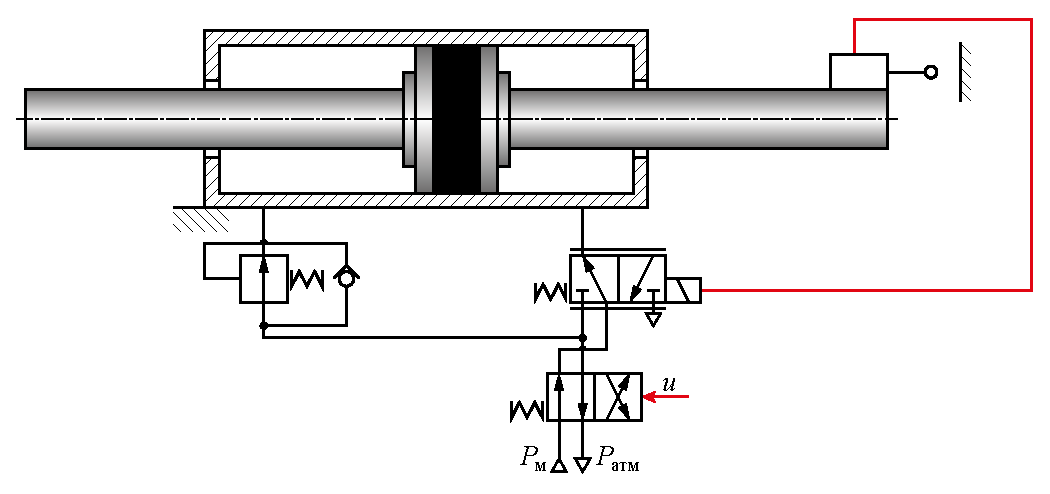
\includegraphics{phillipov_pp.eps}
	\caption{Схема позиционного пневмопривода}\label{fig:phillipov_positioning}
\end{figure}

Принципиальной особенностью предложенной Филипповым системы является комбинирование релейного и следящего режимов
работы: релейный режим используется на участках разгона и установившегося движения, а следящий -- при торможении и
точном позиционировании. Такой подход, реализованный за счет введения
пропорционального распределителя и датчика обратной связи, обеспечивает возможность
позиционирования в произвольной точке хода поршня. При этом параметры привода адаптивно
изменяются в зависимости от текущей координаты позиционирования, что позволяет обеспечить требуемую
точность останова и устойчивость системы \cite*{shortnikov:a}.

% Возрастающие требования к точности позиционирования и быстродействию электропневматических систем определяют
% необходимость учета их специфических особенностей при проектировании. Позиционные пневмоприводы, являясь
% системами с переменной структурой, характеризуются существенной нелинейностью динамических процессов и
% параметрической нестабильностью в процессе работы, что требует разработки специальных подходов к их
% исследованию и эксплуатации.

Работы Филиппова заложили фундаментальные основы создания позиционных пневмоприводов с переменной структурой. Дальнейшее развитие
этого направления осуществлялось в рамках двух основных задач: повышение быстродействия привода и обеспечение
точности позиционирования. При этом особое внимание уделялось проблеме эффективного торможения после участка
разгона, поскольку именно этот этап во многом определяет итоговую точность позиционирования.

В области повышения быстродействия существенный вклад внесли исследования Е.В. Герц.
В работах \cite*{герц:скоростной_привод,герц:групповой_привод} Е.В. Герц исследует проблему повышения быстродействия пневматических
приводов в машиностроении. На основе разработанных математических моделей показано, что типовые промышленные пневмоприводы обладают
недостаточной скоростью рабочих органов (\num{0.5}~--~1 \si{\metre\per\square\second}), что не удовлетворяет требованиям ряда технологических процессов,
где необходима скорость 5~--~20 \si{\metre\per\square\second}.
Для решения данной проблемы предложено использование высокоскоростных пневмоприводов со встроенной полостью-резервуаром. Основной принцип повышения скорости
заключается в обеспечении значительного перепада давлений на рабочем поршне: в рабочей полости поддерживается давление близкое
к магистральному (0,5~--~0,7 \si{\mega\pascal}), а в выхлопной – атмосферное.
Исследования показали существенные преимущества таких пневмоприводов: увеличение рабочего усилия и скорости поршня (до \num{5.3} \si{\metre\per\square\second} на коротких ходах),
повышение энергетической эффективности, возможность точной регулировки выпуска воздуха из резервуара. Однако
их конструкция сложнее типовых и требует больших затрат на подготовку и расход сжатого воздуха.
Несмотря на указанные недостатки, использование высокоскоростных пневмоприводов со встроенным резервуаром признано эффективным
решением для повышения быстродействия в ответственных технологических процессах машиностроения.

В работе \cite*{божкова:повышение_быстродействия} рассматривался выбор
оптимальных параметров управления пневматическим приводом промышленного робота.
Целью было обеспечение высокой скорости работы при сохранении требуемой точности позиционирования.

Авторы Л.В. Божкова и О.А. Дащенко предложили повысить быстродействие путем одновременной работы
динамически независимых узлов привода. Это позволяет избежать последовательной активации пневматических двигателей,
что является типичной практикой для современных промышленных роботов.

Для реализации программного управления без обратной связи, авторы дают ряд рекомендаций по наладке системы.
Это позволяет сократить время переналадки, обеспечить плавность и безударность движения. Таким образом, предложенный
подход направлен на повышение производительности промышленных
роботов с пневматическим приводом без ущерба для точности позиционирования.

В патенте Е.А. Рязанова \cite*{патент:рязанов} предложена конструкция позиционного пневмопривода,
в которой управляющая полость исполнительного пневмоцилиндра сообщена с регулируемым
дозатором в виде плавающего поршня с дросселирующим каналом. Запорный элемент входной
камеры дозатора жестко связан с плавающим поршнем, а выходная камера дозатора постоянно
сообщена с управляющей полостью пневмоцилиндра.

Повышение производительности пневмопривода достигается благодаря созданию управляемого
перепада давления на быстроперемещающемся плавающем поршне дозатора из-за дросселирования
потока через канал, а также за счет упрощения конструкции путем организации жесткой связи запорного элемента
с поршнем и обеспечения быстрой прямой подачи рабочей среды из выходной камеры дозатора в
управляющую полость цилиндра. Это ускоряет процессы подачи и перекрытия рабочей среды, повышая
быстродействие и производительность пневмопривода.

В патенте А.А. Кистиченко \cite*{патент:Кистиченко} представлен подход к повышению
быстродействия пневмопривода за счет совершенствования
систем управления. Предложенная конструкция основана на специальной схеме управления пневмораспределителями
и пневмоклапанами, обеспечивающей быстрый выхлоп рабочей среды из полостей пневмоцилиндра при реверсе движения поршня.

В традиционных пневмоприводах необходимость создания разности давлений в рабочих полостях при реверсировании
приводит к выстою поршня, снижающему быстродействие. Предложенное решение устраняет этот недостаток путем управляемой
отсечки полостей цилиндра от магистрали слива. При подходе поршня к точке реверса система поддерживает такой уровень
давления, который обеспечивает быстрое преодоление сил трения и ускорение в обратном направлении.

Управление осуществляется программным устройством на основе информации о положении поршня и давлениях в полостях. Применение
данной конструкции позволяет повысить быстродействие в 3~--~5 раз по сравнению с традиционными решениями.

Развитие пневмопривода шло по пути повышения ускорения и максимальной скорости движения рабочих органов.
Это достигалось за счет использования более совершенных конструкций, обеспечивающих значительный перепад
давлений на поршне, а также совершенствования систем управления для оптимизации процессов реверсирования
движения поршня. Эти исследования позволяли существенно увеличить скорость и ускорение рабочих органов по
сравнению с типовыми решениями.

Параллельно развивалось направление, связанное с совершенствованием систем позиционирования. Здесь следует отметить работы А.А. Парой,
который является одним из первопроходцев в области исследования задач торможения и позиционирования пневмоприводов промышленных роботов.
В своей работе \cite*{парой:способы_торможения} автор статьи отмечает,
что более 40\%
современных промышленных роботов используют пневматические приводы, что объясняется их высокой надежностью и
низкой стоимостью. Пневмоприводы применяются в качестве основного привода в промышленных роботах с
циклическим управлением и грузоподъемностью до 20~$\div$~30~\si{\kilogram}. Конструктивное решение таких роботов
предполагает использование длинноходовых пневмоцилиндров, которые позволяют реализовать режим
торможения в конце хода с помощью специальных тормозных устройств.

Согласно работе, существует два наиболее распространенных способа обеспечения необходимого
тормозного усилия за счет изменения давления в выхлопной полости пневмопривода. Первый способ заключается в
резком уменьшении площади сечения выхлопного отверстия в определенной точке хода с
последующим поддержанием этой площади постоянной до конца хода. Второй способ предполагает
полное перекрытие площади сечения выхлопного отверстия на первом этапе торможения с последующим
открытием до определенной величины и уменьшением до нуля по определенному закону на втором этапе.
Автор статьи предлагает рассмотреть график, иллюстрирующий эти два режима (рисунок \cref*{fig:парой_режимы_торможения}).

\begin{figure}[h]
	\centerfloat
	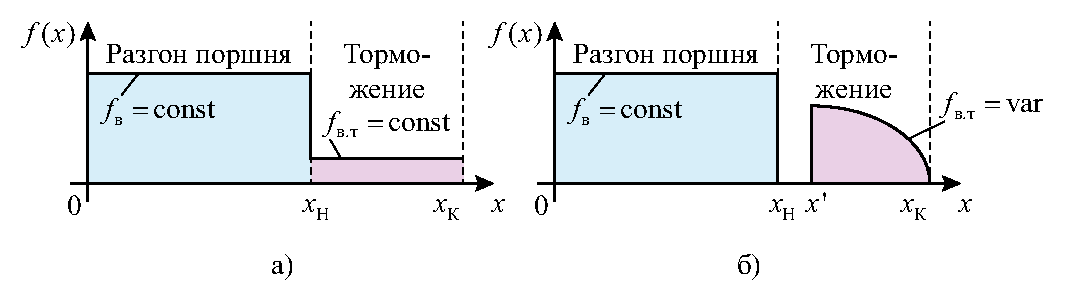
\includegraphics{paroy_brake_mode.eps}
	\caption{Режимы торможения}\label{fig:парой_режимы_торможения}
\end{figure}

Для проектирования тормозных устройств, использующих указанные способы, необходимо определить ряд
параметров, таких как координата начала торможения, площадь сечения выхлопного отверстия,
а также дополнительные координаты и закон изменения площади выхлопа для второго способа.
Автор статьи приводит математические модели, основанные на термодинамических и механических законах,
для расчета этих параметров.

Обобщение накопленного опыта также нашло отражение в разработках Филиппова, где были предложены комплексные решения с использованием
тормозных устройств. В своей монографии, И.Б. Филиппов \cite*{филипов:тормозные_устройства} подробно рассмотрел конструкции и
принципы построения тормозных устройств, применяемых преимущественно для торможения рабочих органов и звеньев машин
с пневмоприводами. Автором была предложена классификация, включающая механические (пружинные, резиновые, эластомерные, инерционные и фрикционные),
пневматические (напорные и вакуумные), гидравлические (дроссельного регулирования), электрические (электромагнитные) и комбинированные тормозные устройства.
Данная класификация представлена на рисунке \cref*{fig:класс_схема_тормозных_устройств}.


\begin{figure}[h]
	\centerfloat
	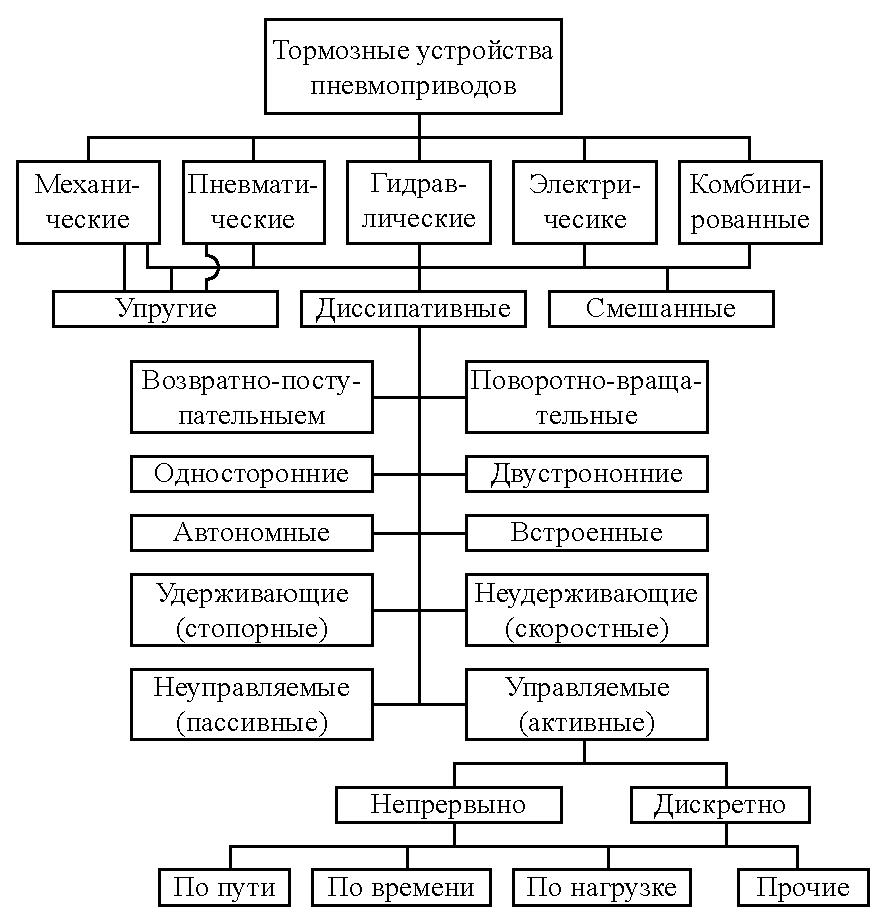
\includegraphics{class_scheme_break.eps}
	\caption{Классификационная схема тормозных устройств}
	\label{fig:класс_схема_тормозных_устройств}
\end{figure}

Выделяются устройства, создающие упругие,
диссипативные или упруго-диссипативные силы сопротивления. Большинство применяемых в настоящее
время тормозных устройств относятся к последнему типу, частично рассеивающих кинетическую энергию и
частично преобразующих ее в потенциальную. Также тормозные устройства могут различаться
по типу движения выходного звена и быть возвратно-поступательными или поворотно-вращательными. Кроме
того они могут быть одностороннего или двустороннего действия. 


Особое внимание в работе уделено автономным управляемым тормозным устройствам, которые могут быть унифицированы
и использованы для торможения движущихся масс механизмов с различными типами приводов. Их применение существенно
упрощает задачи компоновки и проектирования, а также эксплуатацию и обслуживание промышленного оборудования.
Автор приводит примеры конструктивного исполнения таких тормозных устройств, в том числе встроенных в пневмоцилиндры
для позиционирования выходного звена.

Помимо этого, в работе изложены основные требования к тормозным устройствам, такие как обеспечение заданного закона
торможения, ограничение ускорений, плавность торможения, высокая надежность и быстродействие, простота и компактность
конструкции, стабильность характеристик и другие. Для оценки эффективности применения тормозных устройств предлагается
использовать показатели, основанные на сравнении кинетической энергии, действующих сил, скоростей, ускорений и других
параметров движения выходного звена до и после их внедрения.

Дальнейшие исследования в области высокоточных быстродействующих пневмоприводов с позиционированием были проведены
В.И. Грищенко и Дао Тхе Аня.

Работа В.И. Грищенко \cite{Grishchenko2010} посвящена разработке позиционного пневмогидравлического привода
с пневмомеханическим контуром управления. Принципиальная особенность привода
заключается в использовании комбинированных пневмогидравлических линий связи и
многофункционального устройства управления на основе вращающегося распределителя.

Конструктивно привод включает силовой пневмоцилиндр, жестко связанный с тормозным
гидроцилиндром, пневмораспределитель, управляющий направлением перемещения исполнительного
механизма, гидрораспределитель, изменяющий структуру гидросистемы, обратный клапан,
регулятор потока и гидроаккумулятор. Ключевым элементом является многофункциональное
устройство управления, содержащее вращающийся распределитель и осевой золотник.

В исходном состоянии поток сжатого воздуха подводится через узел подготовки воздуха к
центральной позиции пневмораспределителя и через распределитель к левому торцу осевого
золотника. При подаче управляющего сигнала поток воздуха поступает в поршневую полость
пневмоцилиндра, обеспечивая ускоренное перемещение исполнительного механизма.

Процесс позиционирования реализуется в три этапа:
\begin{itemize}
	\item разгон выходного звена привода до максимально возможной скорости (\num{1,5}~$\text{м}\cdot\text{с}^{-1}$);
	\item переход на скорость позиционирования путем изменения структуры привода;
	\item установившееся движение на низкой скорости с последующим точным остановом.
\end{itemize}

Автор предложил оригинальное решение по управлению процессом
позиционирования -- использование пневматических линий связи вместо традиционных гидравлических.
Это позволило повысить быстродействие управляющего устройства благодаря более низкой
вязкости воздуха по сравнению с рабочей жидкостью.

Важным практическим результатом работы явилось установление зависимости точности позиционирования
от кинематических параметров привода. Показано, что при увеличении скорости позиционирования
с \num{5} до \num{20}~\si{\milli\metre\per\second} точность остановки исполнительного механизма изменяется от \num{0,01}
до \num{0,05}~\si{\milli\metre}.
При этом поле рассеивания точности не превышает 10~\si{\micro\metre}.

Промышленная апробация подтвердила эффективность предложенного решения. В
координатно-сверлильном полуавтомате достигнута точность позиционирования
по осевой координате \num{0.03}~--~\num{0.04}~\si{\milli\metre} при разбросе выбега \num{0.01}~\si{\milli\metre}.\
В автоматизированном сварочном комплексе обеспечена точность позиционирования
соединений труба-втулка \num{0.1}~--~\num{0.26}~\si{\milli\metre} при различных типоразмерах труб.

В работе Дао Тхе Аня \cite{DaoTheAnh2016} предложен позиционный пневмопривод
повышенного быстродействия и точности.
Автором разработана оригинальная структура привода, включающая силовой пневмоцилиндр, пневмомеханический
контур управления с многопараметрическим датчиком и внешнее тормозное устройство.

В качестве ключевого элемента системы управления используется многопараметрический
пневмомеханический датчик, который преобразует поступательное движение штока пневмоцилиндра
во вращательное движение модулятора через зубчатую передачу. При вращении модулятора формируется
последовательность импульсов давления, несущих информацию о параметрах движения: количество импульсов
пропорционально перемещению, частота -- скорости, амплитуда -- действующей нагрузке. Это обеспечивает
контроль процесса позиционирования в реальном времени.

Особенностью предложенного привода является применение внешнего тормозного устройства с фрикционными
накладками из специальных материалов (Арголон-ТХ, carbenix-4000). Управление тормозом осуществляется
пневматически через электромагнитный распределитель. Такое решение обеспечивает эффективное торможение
и надежную фиксацию механизма в заданной позиции.
Для описания динамики привода автором разработана обобщенная математическая модель в виде системы нелинейных
дифференциальных уравнений. Модель учитывает взаимодействие электромагнитной подсистемы пневмораспределителя,
силовой подсистемы и подсистемы торможения. Проведенные экспериментальные исследования подтвердили адекватность модели.

В результате исследований на специальном стенде установлено, что точность
позиционирования привода составляет \num{40}~--~\num{130}~\si{\micro\metre} при перемещаемых массах
\num{10}~--~\num{17}~кг,
что в \num{2.25} раза превышает показатели серийных пневмоприводов. При этом время
позиционирования сокращено в \num{1.25} раза по сравнению с традиционными решениями.

Разработанное автором программное обеспечение для управления приводом реализовано
на базе программируемого логического контроллера DVP-28SV. Программа формирует
управляющие воздействия на электромагнитные распределители в соответствии с
сигналами датчика и заданным алгоритмом работы. Практическая значимость разработки
подтверждена внедрением в производственную практику ООО <<Камоцци Пневматика>>, где
использование предложенной методики расчета обеспечило сокращение затрат времени и
средств на проектирование приводов на 23\%.






\section{Позиционные пневмоприводы с дискретными распределителями}

Проведенный анализ развития позиционных пневмоприводов показывает, что многие существующие
решения основаны на применении пропорциональной техники,
обеспечивающей плавное регулирование расхода воздуха. Однако в современных условиях особую актуальность приобретает
задача создания систем на базе дискретных распределителей, что обусловлено их существенно меньшей
стоимостью, более высокой надежностью и лучшей совместимостью с цифровыми системами управления.

Характерной особенностью позиционных пневмоприводов с дискретными распределителями является то, что они могут рассматриваться как системы с переменной
структурой. В процессе работы такие системы претерпевают качественные изменения своей структуры, обусловленные переключением распределителей, что приводит к
существенному изменению динамических свойств привода на различных этапах движения.

Проведенный анализ современного состояния исследований выявил существенные пробелы в текущем понимании проблемы функционирования
таких систем. В первую очередь отсутствует комплексный подход к оценке эффективности различных структур позиционных пневмоприводов с дискретными распределителями.
Существующие публикации, как правило, фокусируются на отдельных показателях качества, таких как точность или быстродействие, без учета их взаимного влияния. При этом
недостаточно исследована проблема взаимосвязи между повышением точности позиционирования и увеличением частоты переключений распределителей, что напрямую влияет на износ оборудования и его ресурс.

Анализ особенностей функционирования этих систем выявляет три противоречивых требования: обеспечение высокой точности
позиционирования, достижение требуемого быстродействия и минимизация количества переключений распределителей. Повышение точности
требует более частого переключения распределителей для коррекции положения штока, что приводит к ускоренному износу распределительной аппаратуры и снижению ресурса системы.
В свою очередь, увеличение быстродействия может негативно сказаться на точности из-за возрастания динамических ошибок, а стремление к минимизации числа переключений ограничивает
возможности как точной коррекции положения, так и обеспечения требуемого быстродействия.

Существующие методики многокритериальной оптимизации параметров таких систем не обеспечивают требуемой эффективности.
Для решения данной задачи целесообразно применение аппарата Парето-оптимизации, позволяющего построить множество недоминируемых решений в
пространстве трех критериев. Построение фронта Парето дает возможность выявить предельно достижимые характеристики системы при различных соотношениях
критериев, научно обосновать выбор рациональных параметров с учетом конкретных требований к точности, быстродействию и ресурсу, а также оценить
эффективность различных структур пневмоприводов с позиции многокритериальной оптимальности.

Управление подобными системами требует особого подхода, учитывающего наличие ограниченного числа возможных состояний, определяемых комбинациями положений
дискретных распределителей. При этом существенная нелинейность динамических процессов, обусловленная как физическими свойствами сжатого воздуха,
так и дискретным характером управляющих воздействий, создает дополнительные сложности при разработке алгоритмов управления.

Для эффективного решения задачи позиционирования принципиально важным является интегративный подход к проектированию таких систем. Попытки оптимизации отдельных подсистем
без учета их взаимного влияния, как показывает практика, не позволяют достичь требуемых показателей качества. Это обусловлено тесной взаимосвязанностью процессов в
пневматической, механической и управляющей подсистемах. Термодинамические процессы в полостях пневмоцилиндра определяют динамику механической части, которая в свою
очередь влияет на алгоритмы переключения распределителей, что в конечном итоге отражается на позиционировании. Такая взаимосвязь исключает возможность независимого
рассмотрения подсистем и требует комплексного подхода к проектированию.

Развитие данного направления можно проследить через ряд исследовательских работ и патентных решений, предлагающих различные подходы к реализации дискретного управления пневмоприводами.

Так, в работе И.Б. Филиппова \cite*{филиппов:позиц_след_пневмопривод} рассматриваются особенности позиционных пневматических механизмов
с дискретным управлением, предназначенных для перемещения выходных звеньев или объектов из точки в точку по
заданной программе. Отмечается, что для таких механизмов основными требованиями являются обеспечение максимального
быстродействия и необходимой точности позиционирования при ограниченных динамических нагрузках.

Описывается конструкция и принцип работы разработанного позиционного пневмопривода с одной дискретно управляемой полостью, представленного
на рисунке \cref*{fig:позиционный_пп_филипов}.

\begin{figure}[h]
	\centerfloat
	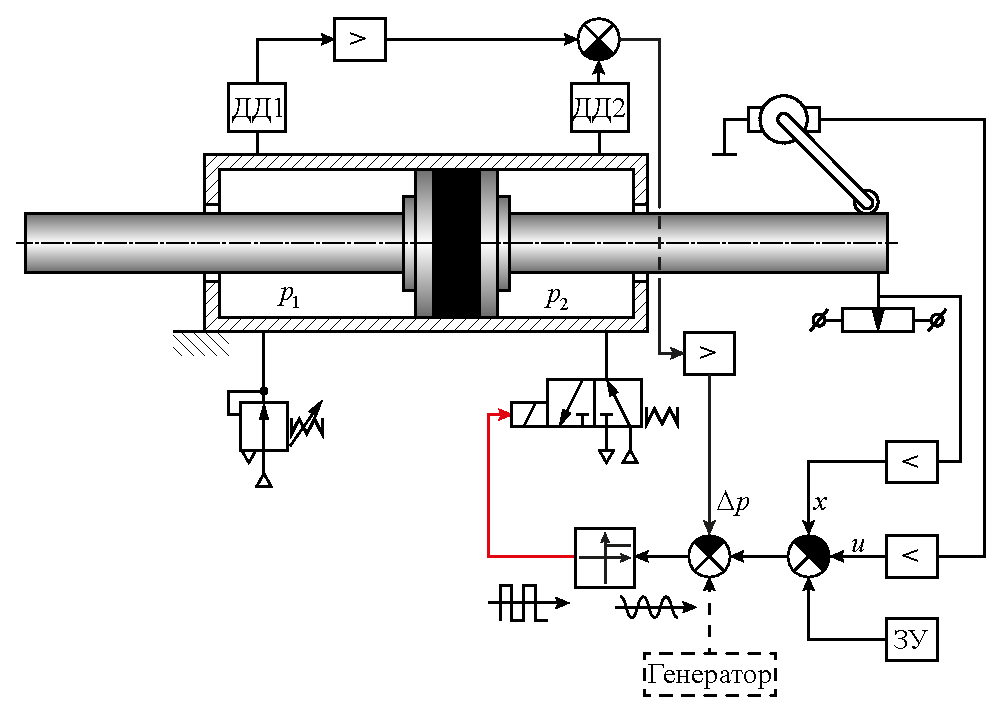
\includegraphics{philipov_positinon_act.eps}
	\caption{Схема дискретного пневмопозиционера}\label{fig:позиционный_пп_филипов}
\end{figure}

Его силовая часть состоит из пневмоцилиндра, в полости 1 которого редукционным клапаном поддерживается
постоянное давление, а в штоковой полости давление определяется положением трехлинейного двухпозиционного распределителя. Измерительная
часть включает датчики давления, тахогенератор и потенциометр для обратных связей по перемещению, скорости и перепаду
давления. Управление движением сводится к управлению торможением и позиционированием за счет переключения распределителя,
соединяющего полость 2 то с магистралью, то с атмосферой.

Автор отмечает, что вследствие колебания давления в полости 2 уменьшается влияние зоны нечувствительности,
определяемой сухим трением. Приведены результаты исследований, показывающие, что частота переключения распределителя определяется
его собственным временем запаздывания и мало зависит от других параметров, что позволяет избежать автоколебаний даже
в наиболее неблагоприятных точках позиционирования.

Дополнительные возможности открывает применение вибрационного сглаживания нелинейностей вынужденными колебаниями.
В этом случае при достижении сигналом рассогласования величины амплитуды гармонического воздействия клапан переходит
в режим постоянного переключения, поддерживая давление в управляемой полости таким, чтобы обеспечить торможение и точное
позиционирование. Преимуществом данного алгоритма является возможность задавать частоту вынужденных колебаний для
обеспечения необходимого качества переходного процесса и требуемого запаса устойчивости.

Дальнейшим шагом стало комплексное рассмотрение Г.А. Крутиковым, А.И. Кудрявцевым и Л.А. Пекарем \cite*{крутиков:способы_торможения_12}
способов торможения поршня пневмопривода без использования специальных тормозных устройств. В работе
рассмотрено 12 схем торможения пневмопривода, разделенные на 3 основные группы (I, II, III), показанные на рисунке \cref*{fig:эффективные_схемы_торможения_12}.

\begin{figure}[h]
    \centerfloat
    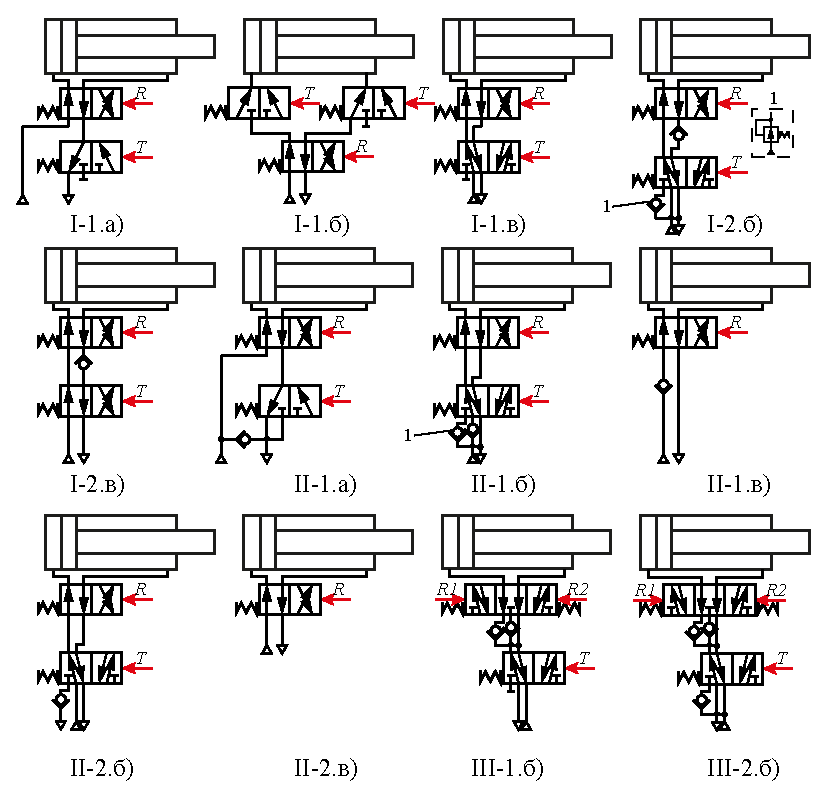
\includegraphics{kurtikob.eps}
    \caption{Эффективные схемы торможения пневмопривода}\label{fig:эффективные_схемы_торможения_12}
\end{figure}

Отличительной особенностью этих схем является отсутствие регулируемых дросселей и емкостей ---
настройка оптимального режима торможения осуществляется только изменением тормозного пути.

Оценка эффективности каждой схемы осуществлялась по ряду ключевых критериев: время срабатывания пневмопривода,
относительная масса сжатого воздуха, потребляемого за один цикл, осредненный за цикл КПД пневмопривода, максимальное
ускорение при торможении, максимальная степень сжатия воздуха в тормозной полости, относительная стоимость
аппаратурной реализации и относительный тормозной путь. Для объективного сравнения каждой схеме была дана оценка в
баллах от 1 до 10 по каждому из показателей, причем максимальный балл присваивался схеме с наилучшим значением
параметра. Коэффициенты значимости различных критериев были определены экспертным методом в соответствии с
рекомендациями.

Наилучшие комплексные показатели качества продемонстрировали схемы III-2.б и III-1.б, которые, несмотря на
более высокую стоимость реализации, обладают лучшими энергетическими характеристиками, высоким быстродействием
и более плавным режимом торможения. Принципиальное отличие этих схем группы III заключается в том, что в них
используется не только вторая составляющая удельной работы сжатого воздуха (изотермическое расширение), но и его
потенциальная энергия, что существенно повышает КПД пневмопривода.

Особого внимания заслуживает схема I-2.б с обратным клапаном, которая позволяет устранить недостатки схемы I-1.б
с высокими пиковыми ускорениями и отскоком поршня. Максимальное ускорение в этом случае снижается с 15,5~\si{\metre\per\square\second}
до 4,16~\si{\metre\per\square\second}, отскок минимален, а время срабатывания составляет 1,05~\si{\second}. Энергетические характеристики также улучшаются
за счет частичной рекуперации воздуха из тормозной полости.

Дальнейшее улучшение режима торможения обеспечивает модификация схемы I-2.б с установкой редукционного клапана вместо
обратного. Это позволяет реализовать практически равнозамедленный режим торможения с постоянным отрицательным
ускорением 1,38~\si{\metre\per\square\second}, полностью устраняет отскок поршня и обеспечивает предохранение тормозной полости от недопустимо
высоких давлений. Основными преимуществами такой схемы являются мягкий и плавный режим торможения с регулируемым
ускорением, экономное использование сжатого воздуха за счет рекуперации, высокое быстродействие и удобство настройки.

Таким образом, комплексная оценка и сравнение различных схем торможения пневмопривода, проведенная авторами, позволила
выявить наиболее эффективные решения. В частности, схема I-2.б с редукционным клапаном демонстрирует оптимальное
сочетание высокого быстродействия, плавного режима торможения с заданным ускорением, экономного расхода сжатого
воздуха и защиты тормозной полости от чрезмерных давлений. Эта схема рекомендуется авторами для использования в качестве
внешнего тормозного устройства для пневмопривода с большими инерционными нагрузками.

В настоящее время, благодаря стремительному развитию микроэлектроники и её применению в различных
областях, стало возможным использование сложных алгоритмов управления. Эти достижения позволяют решать
многие отмеченные ранее вопросы с помощью более гибких систем управления.

Однако применение алгоритмов, предназначенных для непрерывных систем, к системам с
дискретными элементами может быть затруднительным или даже невозможным. Часто при использовании
ПИД-регулятора исследователи применяют различные преобразователи и модуляции сигнала. Например,
широко распространено использование широтно-импульсной модуляции (ШИМ) в сочетании с ПИД.

% \section{Улучшение управляющих структру пневмопривода}\label{subsec:ch1/sec5/subsec1}

В работе Варсевельда \cite*{pwm:Varseveld} подробно рассмотрена разработка системы позиционного пневмопривода, схема которого представлена на
рисунке \ref*{fig:позиционный_пп_pwm}, с использованием недорогих
дискретных распределителей с электромагнитным управлением, вместо дорогостоящих пропорциональных. Особое внимание уделено
проектированию системы управления, обеспечивающей высокое быстродействие и точность позиционирования.

\begin{figure}[htpb]
    \centerfloat
    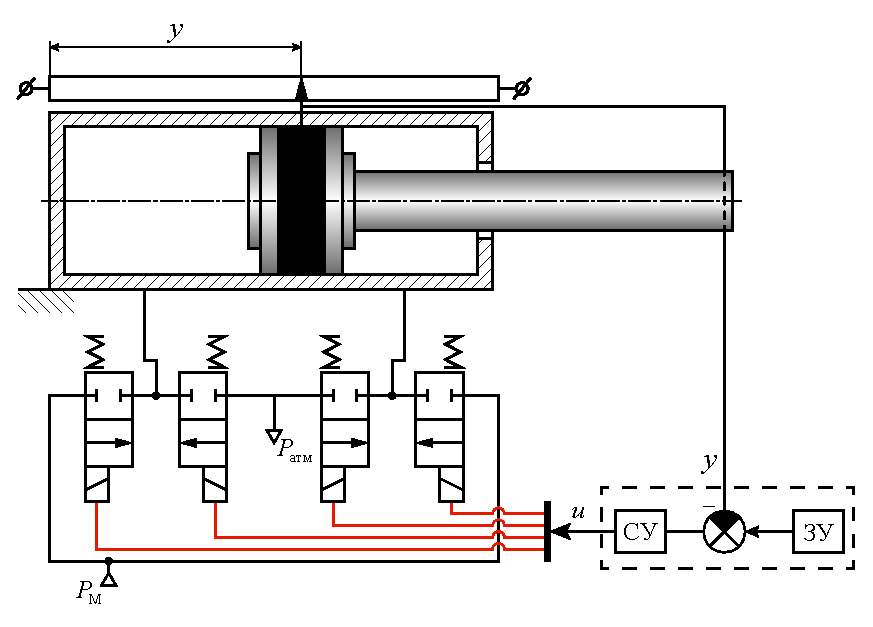
\includegraphics{positioning_actuator_pwm_ov.eps}
    \caption{Схема позиционного ПП с дискретными распределителями}\label{fig:позиционный_пп_pwm}
\end{figure}

Авторами предложен новый алгоритм с использованием широтно-импульсной модуляции для управления распределителями, позволяющий
получить практически симметричную и линейную характеристику скорости рабочего органа пневмопривода в зависимости от управляющего сигнала.
Это достигается за счет согласованного управления магистральными и выхлопными распределителями, что компенсирует асимметрию,
вызванную разницей активных площадей поршня в поршневой и штоковой полостях. Экспериментальные исследования подтвердили высокую линейность и
симметрию полученной характеристики.

На основе экспериментальных данных авторами синтезирована линейная авторегрессионная модель пневмопривода.
Анализ модели показал, что демпфирование системы существенно зависит от положения поршня, достигая минимума в
центральной части хода. Это объясняется наличием сухого кулоновского трения.

Для компенсации влияния трения в систему управления введен ПИД-регулятор с дополнительной компенсацией
трения и интегральной составляющей ограниченной с двух сторон. Применение этих мер позволило существенно уменьшить статическую
ошибку позиционирования.

В ходе экспериментальных исследований авторам удалось достичь высокого быстродействия системы управления --
время нарастания составило всего 180~\si{\milli\second}. При этом статическая ошибка позиционирования не превышала 0,21~
\si{\milli\metre},
что сопоставимо с результатами, полученными другими исследователями
\cite*{Varseveld:article1,Varseveld:article2,Varseveld:article3,Surgenor1997ContinuousSM},
использовавшими более дорогостоящие
пропорциональные распределители. Кроме того, система продемонстрировала инвариантность к шестикратному изменению
инерционной нагрузки. Авторы также показали возможность точного отслеживания $S$-образных траекторий с ошибкой не
более 2~\si{\milli\metre}.

Работа М. Шие \cite*{Shiee} посвящена сравнительному анализу различных схем ШИМ для улучшения позиционирования пневмопривода. Авторы рассматривают пять
основных ШИМ-схем представленных на рисунке \ref*{fig:схемы_шим}.

\begin{figure}[ht]
    \centerfloat{
        \subcaptionbox[List-of-Figures entry]{\label{fig:схемы_шим-1}}{
            \begin{tikzpicture}
                \begin{axis}[
                        width = 8cm,
                        height = 5cm,
                        xmin=-100, xmax=100,
                        ymin=0, ymax=100,
                        xlabel={Сигнал, \%},
                        ylabel={Ширина ШИМ, \%},
                        grid=major,
                        extra tick style={grid=none, draw opacity=0},
                        tick style={line width=0.75pt},
                        axis line style={line width=1pt},
                    ]
                    \addplot[black, mark=none, line width=0.75pt] coordinates {
                            (-100, 0)
                            (100, 100)
                        };
                    \addplot[black, mark=none, line width=0.75pt, dashed] coordinates {
                            (-100, 100)
                            (100, 0)
                        };
                    %add legend
                    \addlegendentry{Расп. 1}
                    \addlegendentry{Расп. 2}


                \end{axis}
            \end{tikzpicture}
        }
        \hfil
        \subcaptionbox[]{\label{fig:схемы_шим-2}}{
            \begin{tikzpicture}
                \begin{axis}[
                        width = 8cm,
                        height = 5cm,
                        xmin=-100, xmax=100,
                        ymin=0, ymax=100,
                        xlabel={Сигнал, \%},
                        ylabel={Ширина ШИМ, \%},
                        grid=major,
                        extra tick style={grid=none, draw opacity=0},
                        tick style={line width=0.75pt},
                        axis line style={line width=1pt},
                    ]
                    \addplot[black, mark=none, line width=0.75pt] coordinates {
                            (-100, 10)
                            (-80, 10)
                            (80, 80)
                            (100, 100)
                        };
                    \addplot[black, mark=none, line width=0.75pt, dashed] coordinates {
                            (-100, 100)
                            (-80, 80)
                            (80, 10)
                            (100, 10)
                        };
                    %add legend
                    \addlegendentry{Расп. 1}
                    \addlegendentry{Расп. 2}


                \end{axis}
            \end{tikzpicture}
        }
        \vfil
        \subcaptionbox[]{\label{fig:схемы_шим-3}}{
            \begin{tikzpicture}
                \begin{axis}[
                        width = 8cm,
                        height = 5cm,
                        xmin=-100, xmax=100,
                        ymin=0, ymax=100,
                        xlabel={Сигнал, \%},
                        ylabel={Ширина ШИМ, \%},
                        grid=major,
                        extra tick style={grid=none, draw opacity=0},
                        tick style={line width=0.75pt},
                        axis line style={line width=1pt},
                    ]
                    \addplot[black, mark=none, line width=0.75pt] coordinates {
                            (-100, 20)
                            (-70, 20)
                            (70, 80)
                            (100, 80)
                        };
                    \addplot[black, mark=none, line width=0.75pt,dashed] coordinates {
                            (-100, 80)
                            (-70, 80)
                            (70, 20)
                            (100, 20)
                        };
                    %add legend
                    \addlegendentry{Расп. 1}
                    \addlegendentry{Расп. 2}
                \end{axis}
            \end{tikzpicture}
        }
        \hfil
        \subcaptionbox[]{\label{fig:схемы_шим-4}}{
            \begin{tikzpicture}
                \begin{axis}[
                        width = 8cm,
                        height = 5cm,
                        xmin=-100, xmax=100,
                        ymin=0, ymax=100,
                        xlabel={Сигнал, \%},
                        ylabel={Ширина ШИМ, \%},
                        grid=major,
                        extra tick style={grid=none, draw opacity=0},
                        tick style={line width=0.75pt},
                        axis line style={line width=1pt},
                    ]
                    \addplot[black, mark=none, line width=0.75pt, ] coordinates {
                            (-100, 20)
                            (0, 20)
                            (100, 80)
                        };
                    \addplot[black, mark=none, line width=0.75pt, dashed] coordinates {
                            (-100, 80)
                            (0, 20)
                            (100, 20)
                        };
                    %add legend
                    \addlegendentry{Расп. 1}
                    \addlegendentry{Расп. 2}
                \end{axis}
            \end{tikzpicture}
        }
        \vfil    \subcaptionbox[]{\label{fig:схемы_шим-5}}{
            \begin{tikzpicture}
                \begin{axis}[
                        width = 8cm,
                        height = 5cm,
                        xmin=-100, xmax=100,
                        ymin=0, ymax=100,
                        xlabel={Сигнал, \%},
                        ylabel={Ширина ШИМ, \%},
                        grid=major,
                        extra tick style={grid=none, draw opacity=0},
                        tick style={line width=0.75pt},
                        axis line style={line width=1pt},
                    ]
                    \addplot[black, mark=none, line width=0.75pt, ] coordinates {
                            (-100, 20)
                            (0, 80)
                            (100, 80)
                        };
                    \addplot[black, mark=none, line width=0.75pt, dashed] coordinates {
                            (-100, 80)
                            (0, 80)
                            (100, 20)
                        };
                    %add legend
                    \addlegendentry{Расп. 1}
                    \addlegendentry{Расп. 2}
                \end{axis}
            \end{tikzpicture}
        }
    }
    \caption{Схемы ШИМ}\label{fig:схемы_шим}
\end{figure}

Схема \cref*{fig:схемы_шим-1} не учитывает динамику включения/выключения распределителей, что приводит к нелинейностям при
крайних значениях входного сигнала. Схема \cref*{fig:схемы_шим-2} учитывает только динамику включения распределителей и добавляет точку перегиба,
чтобы минимизировать ширину импульса ниже определенного значения. Схема \cref*{fig:схемы_шим-3} учитывает как задержку включения, так и
задержку выключения распределителей, вводя два пограничных значения для ширины импульса. Схема \cref*{fig:схемы_шим-4} является модифицированным
вариантом схемы \cref*{fig:схемы_шим-1}, учитывающим задержки клапанов, и обеспечивает меньшую сумму коэффициентов заполнения сигнала поступающего на распределитель,
особенно вблизи нулевого входного сигнала. Схема \cref*{fig:схемы_шим-5} представляет собой модификацию схемы \cref*{fig:схемы_шим-3} с
учетом задержек включения
и выключения клапанов, давая большую суммарную ширину импульса вблизи нулевого входа.

Авторы провели ряд экспериментов со ступенчатыми и гармоническими входными воздействиями, чтобы изучить характеристики
различных ШИМ-схем. По характеристикам позиционирования при ступенчатом входе, схема \cref*{fig:схемы_шим-1} показала наименьшее время
нарастания, но большую статическую ошибку позиционирования, схема \cref*{fig:схемы_шим-4} продемонстрировала наименьшее перерегулирование,
но худшую ошибку, а схема \cref*{fig:схемы_шим-5} имела самое большое время нарастания и ошибку.
При отслеживании гармонического сигнала, первые три схемы показали близкие результаты по среднеквадратичной
ошибке, в то время как схемы \cref*{fig:схемы_шим-4} и \cref*{fig:схемы_шим-5} имели большую ошибку слежения. Эксперименты с увеличением нагрузки показали,
что схема \cref*{fig:схемы_шим-4}
оказалась наименее устойчивой к увеличению инерционной нагрузки, а схема \cref*{fig:схемы_шим-5}, имеющая высокое рабочее давление,
продемонстрировала наибольшую
устойчивость.

Чтобы компенсировать влияние различий в эффективных площадях, авторы предложили модифицированные версии каждой ШИМ-схемы.
Модификация заключается в сдвиге диаграмм ШИМ-схем с целью достижения нулевой выходной силы при нулевом входном сигнале.

Экспериментальные результаты при ступенчатом входном воздействии продемонстрировали, что модифицированные ШИМ-схемы, особенно для схем \cref*{fig:схемы_шим-1},
\cref*{fig:схемы_шим-2}, \cref*{fig:схемы_шим-3} и \cref*{fig:схемы_шим-5}, обеспечивают значительное улучшение характеристик позиционирования,
в частности, снижение статической ошибки позиционирования. Это связано с тем, что при высоких рабочих давлениях различия в эффективных площадях поршня
становятся более значимыми, и предложенные модификации эффективно компенсируют этот эффект.

В статье Трана Динь Сона \cite*{Tran:pwm} авторами представлен модифицированный метод позиционного управления
пневмоприводом с использованием четырех дискретных электромагнитных распределителей, схема пневмопривода аналогична схеме
представленной на рисунке \cref*{fig:позиционный_пп_pwm}.

Первоначально в работе проведен анализ алгоритма, разработанного Трунг Куай Нгуеном \cite*{Truong}
в 2007 году. Установлено, что данный алгоритм демонстрирует существенно
перерегулирование при задании малых смещений поршня, что обусловливает необходимость
дальнейшего совершенствования методов управления.

С целью повышения качества позиционирования авторами была предложена модификация
алгоритма. Ключевым аспектом модификации стало разделение диапазона задаваемых
положений на две области: малые смещения $(x_d \leqslant \text{50}~\si{\milli\metre})$
и большие смещения $(x_d > \text{50}~\si{\milli\metre})$.
Для каждой области авторами разработаны индивидуальные законы управления с использованием
семи различных режимов работы четырех электромагнитных распределителей в сочетании с ШИМ.

Для диапазона малых смещений при значительной ошибке позиционирования
$e \leqslant -\alpha$ авторами
введен новый режим $M_6$, предполагающий одновременное открытие двух распределителей, что обеспечивало
плавное низкоскоростное движение. В области промежуточных ошибок
$-\alpha < e < -\beta$ применялся режим
$M_2$ с импульсным открытием одного из распределителей, способствующий быстрому замедлению движения и
устранению перерегулирования.

Для диапазона больших смещений авторами модифицированы режимы $M_2$ и $M_2$ контроллера
посредством организации поочередного импульсного открытия распределителей. Данный подход позволял
плавно замедлять движение поршня.

Экспериментальные исследования подтвердили, что модифицированный алгоритм обеспечивает
существенное улучшение качества позиционного управления по сравнению с исходным алгоритмом,
особенно при отработке малых смещений. Более того, при частотах задающего воздействия
до \num{0.1}~\si{\hertz} модифицированный алгоритм продемонстрировал сопоставимые или превосходящие
характеристики относительно алгоритма для пневмопривода с пропорциональными
распределителями. Однако при более высоких частотах (например, \num{0.5}~\si{\hertz}) характеристики модифицированного
алгоритма значительно ухудшались, что связано с ограниченной скоростью переключения
используемых распределителей.

Таким образом, результаты проведенного исследования свидетельствуют о том, что предложенный
модифицированный алгоритм позволяет существенно повысить качество позиционного управления
пневматическим приводом с дискретными распределителями при низких и средних частотах задающего
воздействия по сравнению с ранее разработанными решениями.

В работе Кайонг Кван Анха \cite*{AHN2005683} так же представлен подход к разработке системы управления пневмоприводом
с использованием дискретных электромагнитных распределителей вместо традиционных пропорциональных распределителей.
Авторы предлагают модифицированный алгоритм ШИМ для точного позиционного управления
пневмоприводом при помощи этих дискретных распределителей.

Центральным элементом разработанной системы управления является трехконтурная схема, представленная на рисунке
\cref*{fig:mpwm_lvqnn},
\begin{figure}[htpb]
    \centerfloat
    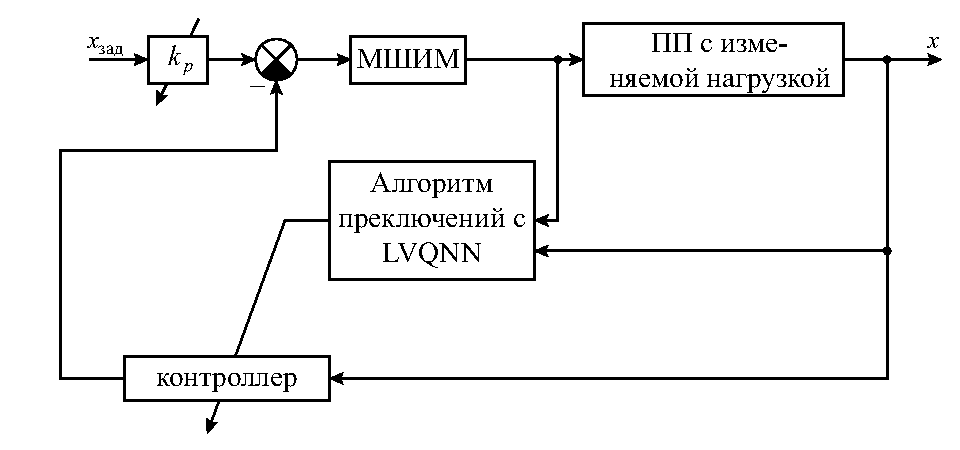
\includegraphics{mpwm_lvqnn.eps}
    \caption{Структурная схема системы управления с МШИМ и LVQNN}\label{fig:mpwm_lvqnn}
\end{figure}
с обратной связью по положению, скорости и ускорению. Такая структура обеспечивает высокое быстродействие и
точность позиционирования. Для адаптации параметров регулятора к изменяющимся внешним нагрузкам авторы применяют
нейронную сеть на основе векторного квантования (LVQNN). Данная интеллектуальная система классификации нагрузки
динамически подстраивает коэффициенты регулятора, компенсируя влияние возмущающих воздействий.

Проведённые экспериментальные исследования подтвердили, что предложенный алгоритм МШИМ обеспечивает точность позиционирования
в пределах \num{0.2}~\si{\milli\metre}, что существенно превосходит результаты стандартного ШИМ-алгоритма (ошибка около \num{1.75}~\si{\milli\metre}). Применение
LVQNN и адаптивной настройки параметров регулятора позволило эффективно компенсировать влияние изменяющейся внешней нагрузки и
добиться высокой стабильности системы управления.

Таким образом, ключевыми элементами разработанной системы управления являются алгоритм МШИМ,
трёхконтурная схема регулирования с обратной связью, а также интеллектуальная система адаптации параметров
регулятора на основе LVQNN. Полученные результаты демонстрируют высокую эффективность предложенных методов для точного
позиционного управления пневматическим пневмоприводом в условиях изменяющихся внешних нагрузок.

Современные подходы к управлению пневмоприводами с дискретными распределителями основаны на
методах управления системами с переменной структурой. Дискретный характер переключений распределителей
формирует различные конфигурации пневматической системы, каждая из которых обладает собственными
динамическими характеристиками. При этом интеллектуальные алгоритмы управления, включая нейронные
сети и нечеткую логику, позволя- ют эффективно адаптировать параметры регулирования к изменениям
структуры привода.

Особую актуальность приобрело применение методов управления в скользящих режимах,
обеспечивающих устойчивое функционирование системы при переходах между различными структурными состояниями.
Данный подход, успешно зарекомендовавший себя в электроприводе, органично соответствует дискретной природе
пневмопривода, где каждое переключение распределителей формирует новую конфигурацию силовой части.


%%%%%%%%%%%%%%%%%%%%%%%%%%%%%%%%%%%%%%%%%%%%%%%%%%%%%%%%%%%%%%%%%%%%%%%%%%%%%%%%%%%%%%%%%%%%%%%%%%%%%%%%%%%%%%%%%%%%%%%%%%%%
%%%%%%%%%%%%%%%%%%%%%%%%%%%%%%%%%%%%%%%%%%%%%%%%%%%%%%%%%%%%%%%%%%%%%%%%%%%%%%%%%%%%%%%%%%%%%%%%%%%%%%%%%%%%%%%%%%%%%%%%%%%%
%%%%%%%%%%%%%%%%%%%%%%%%%%%%%%%%%%%%%%%%%%%%%%%%%%%%%%%%%%%%%%%%%%%%%%%%%%%%%%%%%%%%%%%%%%%%%%%%%%%%%%%%%%%%%%%%%%%%%%%%%%%%

% \subsection{Исследование управления в скользящих режимах}\label{subsec:ch1/sec5/subsec2}

Управление в скользящих режимах \cite*{utkin2017sliding} -- это класс нелинейных методов управления, которые делают систему управления разрывной.
Процесс проектирования делится на два этапа: выбор поверхностей переключения для желаемого режима движения и синтез разрывного
управления для движения системы по этим поверхностям.

Движение системы по поверхностям переключения обладает рядом преимуществ: снижение порядка системы, инвариантность
к параметрическим и внешним возмущениям. Для описания движения используются специальные математические методы, такие
как регуляризация и метод эквивалентного управления.

%%%%%%%%%%%%%%%%%%%%%%%%%%%%%%%%%%%%%%%%%%%%%%%%%%%%%%%%%%%%%%%%%%%%%%%%%%%%%%%%%%%%%%%%%%%%%%%%%%%%%%%%%%%%%%%%%%%%%%%%%%%%


В статье \cite*{Elsayed} рассматривается исследование, посвящённое управлению положением рабочего органа пневмопривода
с использованием дискретных распределителей.
Авторы предлагают использование алгоритма управления скользящим режимом с коррекцией ошибки регулирования (SMCE), который использует
ШИМ для управления распределителями.

Для управления движением пневматического цилиндра авторы используют только три режима работы
четырёх распределителей, представленные ниже:
\begin{itemize}
    \item режим 1 -- выдвижение штока;
    \item режим 2 -- задвижение штока;
    \item режим 3 -- удержание положения штока;
\end{itemize}

С целью оптимизации параметров SMCE и ПИД-регулятора была разработана модель в Simulink.
Экспериментальные исследования проводились на стенде. Результаты моделирования и экспериментов
показывают, что SMCE обеспечивает более высокую точность
позиционирования, меньшее время установления и меньший выброс по сравнению с традиционным ПИД-регулятором.
Для гармонического входного сигнала среднеквадратичная ошибка при использовании SMCE составляет \num{0.22}~\si{\milli\metre}, а
для ПИД -- \num{0.69}~\si{\milli\metre}. Максимальная абсолютная ошибка для SMCE составляет \num{0.66}~\si{\milli\metre},
а для ПИД -- \num{1.46}~\si{\milli\metre}. Таким образом,
предложенный метод SMCE показал своё превосходство над ПИД-регулятором при управлении положением РО ПП.
%%%%%%%%%%%%%%%%%%%%%%%%%%%%%%%%%%%%%%%%%%%%%%%%%%%%%%%%%%%%%%%%%%%%%%%%%%%%%%%%%%%%%%%%%%%%%%%%%%%%%%%%%%%%%%%%%%%%%%%%%%%%

Статья \cite*{Hodgson:article1} также посвящена разработке алгоритма управления в скользящих режимах
для регулирования пневмопривода
с четырмя дискретными распределителями.
Ключевым отличием от предыдущих работ является расширение числа доступных дискретных режимов управления
с трех до семи.

В основе работы (см. рисунок \ref*{fig:actuators_scheme}) контроллера лежит скользящая поверхность $s$, которая определяется как функция ошибки позиционирования $e$,
её производной и второй производной. Авторы вводят семь возможных режимов переключения распределителей $(M_1 \div M_7)$,
выбор которых производится в зависимости от текущего значения $s$ и eё производной. Диаграмма переходов
представлена на рисунке.

\begin{figure}[ht]
    \centerfloat{
        \begin{tikzpicture}[auto]
            \usetikzlibrary {matrix,positioning,shapes.misc,arrows,shapes.geometric,graphs,backgrounds,arrows.meta}
            \tikzstyle{main_block} = [rectangle, rounded corners=0.5cm, draw, text centered, minimum height=4em, line width=1pt, text width=6em]
            \tikzstyle{text_block} = [rectangle, rounded corners=0.25cm, text centered, fill=white]
            \tikzstyle{cond_block} = [diamond, text centered, draw, text centered, line width = 1pt]
            \tikzstyle{arr} = [-triangle 45, line width=1pt]
            \tikzstyle{line} = [-, line width=1pt]
            % \tikzstyle{dashed} = [-triangle 45, line width=1pt, dashed]
            \matrix [column sep=3mm, row sep=7mm]
            {
                                                                              &
                                                                              &
                \node[main_block] (M7) {$M_7$\\$P_1$ -- оп.\\$P_2$ -- нап.};    \\
                %
                \node[text_block] (t1_0) {$\beta$};                           &
                \node[text_block] (t1_1) {$s > \beta$};                       &
                \node[text_block] (t1_2) {$s > \beta$};                       &
                \node[text_block] (t1_3) {$s > \beta$};                         \\
                %
                                                                              &
                \node[main_block] (M5) {$M_5$\\$P_1$ -- зап.\\$P_2$ -- нап.}; &
                \node[cond_block] (C1) {$E_1 > 1$};                           &
                \node[main_block] (M3) {$M_3$\\$P_1$ -- оп.\\$P_2$ -- зап.};    \\
                %
                \node[text_block] (t2_0) {$\epsilon$};                        &
                \node[text_block] (t2_1) {$s < \epsilon$};                    &
                \node[text_block] (t2_2) {$s > \epsilon$};                    &
                \node[text_block] (t2_3) {$s < \epsilon$};                      \\
                %
                                                                              &
                                                                              &
                \node[main_block] (M1) {$M_1$\\$P_1$ -- зап.\\$P_2$ -- зап.};   \\
                %
                \node[text_block] (t3_0) {$-\epsilon$};                       &
                \node[text_block] (t3_1) {$s > -\epsilon$};                   &
                \node[text_block] (t3_2) {$s < -\epsilon$};                   &
                \node[text_block] (t3_3) {$s > -\epsilon$};                     \\
                %
                                                                              &
                \node[main_block] (M2) {$M_2$\\$P_1$ -- нап.\\$P_2$ -- зап.}; &
                \node[cond_block] (C2) {$E_1 > 1$};                           &
                \node[main_block] (M4) {$M_4$\\$P_1$ -- зап.\\$P_2$ -- оп.};    \\
                %
                \node[text_block] (t4_0) {$-\beta$};                          &
                \node[text_block] (t4_1) {$s < -\beta$};                      &
                \node[text_block] (t4_2) {$s > -\beta$};                      &
                \node[text_block] (t4_3) {$s < -\beta$};                        \\
                %
                                                                              &
                                                                              &
                \node[main_block] (M6) {$M_6$\\$P_1$ -- нап.\\$P_2$ -- оп.};    \\
                %%%%%%%%%%%%%%%%%%%%%%%%%%%%%%%%%%%%%%%%%%%%%%%%%%%%%%%%%%%%%%%%%%%%
            };
            \begin{scope}[on background layer]
                \draw[arr] (M7.south) -- (C1);
                \draw[line] (M5.north) -- (t1_1);
                \draw[arr] (t1_1.north) to [out=90,in=180]  (M7.west);
                \draw[line] (M3.north) -- (t1_3);
                \draw[arr] (t1_3.north) to [out=90,in=0] (M7.east);

                \draw[arr] ([xshift=1cm]M5.north) to [out=90,in=90] node[below] {$\tau$} (C1.north);
                \draw[arr] ([xshift=-1cm]M3.north) to [out=90,in=90] node[below] {$\tau$} (C1.north);
                %%%%%%%%%%%%%%%%%%%%%%%%%%%%%%%%%%%%%%%%%%%%%%%%%%%%%%%%%%%%%
                \draw[line, loosely dashed] (t1_0.east) -- ([xshift=3cm]t1_3.west);
                \draw[line, loosely dashed] (t2_0.east) -- ([xshift=3cm]t2_3.west);
                \draw[line, loosely dashed] (t3_0.east) -- ([xshift=3.4cm]t3_3.west);
                \draw[line, loosely dashed] (t4_0.east) -- ([xshift=3.4cm]t4_3.west);

                \draw[line] (M5.south) -- (t2_1.north);
                \draw[line] (M3.south) -- (t2_3.north);
                %%%%%%%%%%%%%%%%%%%%%%%%%%%%%%%%%%%%%%%%%%%%%%%%%%%%%%%%%%%%%
                \draw[arr] (C1.west) -- (M5.east);
                \draw[arr] (C1.east) -- (M3.west);

                \draw[arr] (t2_1.south) to [out=-90,in=180]  (M1.west);
                \draw[arr] (t2_3.south) to [out=-90,in=0] (M1.east);

                \draw[arr] (M1.north) -- (C1.south);
                %%%%%%%%%%%%%%%%%%%%%%%%%%%%%%%%%%%%%%%%%%%%%%%%%%%%%%%%%%%%%

                \draw[arr] (M1.south) -- (C2);
                \draw[line] (M2.north) -- (t3_1);
                \draw[arr] (t3_1.north) to [out=90,in=180]  (M1.west);
                \draw[line] (M4.north) -- (t3_3);
                \draw[arr] (t3_3.north) to [out=90,in=0] (M1.east);

                \draw[arr] ([xshift=1cm]M2.south) to [out=-90,in=-90] node[above] {$\tau$} (C2.south);
                \draw[arr] ([xshift=-1cm]M4.south) to [out=-90,in=-90] node[above] {$\tau$} (C2.south);

                \draw[arr] (M6.north) -- (C2.south);

                \draw[line] (t4_1.north) --  (M2.south);
                \draw[line] (t4_3.north) --  (M4.south);

                \draw[arr] (t4_1.south) to [out=-90,in=180]  (M6.west);
                \draw[arr] (t4_3.south) to [out=-90,in=0] (M6.east);

                \draw[arr] (C2.west) -- (M2.east);
                \draw[arr] (C2.east) -- (M4.west);

                \draw[arr] ([xshift=-6cm]M6.south) -- node {$s$} ([xshift=-6cm]M7.north);

                % %%%%%%%%%%%%%%%%%%%%%%%%%%%%%%%%%%%%%%%%%%%%%%%%%%%%%%%%%%%%%
                % \draw[line, loosely dashed] (t1_0.east) -- ([xshift=3cm]t1_3.west);
                % \draw[line, loosely dashed] (t2_0.east) -- ([xshift=3cm]t2_3.west);
                % \draw[line, loosely dashed] (t3_0.east) -- ([xshift=3.4cm]t3_3.west);
                % \draw[line, loosely dashed] (t4_0.east) -- ([xshift=3.4cm]t4_3.west);
            \end{scope}
        \end{tikzpicture}
    }
    \caption{Диаграмма переключения режимов }\label{fig:actuators_scheme}
\end{figure}

Режимы $M_7$ и $M_6$ применяются при больших по модулю значениях $s$ для обеспечения максимальных ускорений в положительном и
отрицательном направлениях соответственно. Эти режимы позволяют быстро сократить большие ошибки позиционирования.

Режимы $M_2, M_3, M_4$ и $M_5$ используются при малых ошибках позиционирования $(\lvert s \rvert < \beta)$. Их применение позволяет снизить частоту
переключений распределителей, что способствует увеличению срока службы пневматической системы.

Для выбора оптимального режима в области малых ошибок авторы вводят дополнительные критерии, основанные на разности давлений
в камерах пневмопривода. Это позволяет определить режим, обеспечивающий максимальное ускорение при минимальном количестве
переключений
распределителей. Кроме того, вводится параметр $\tau$, задающий минимальное время между переключениями в этой области, что также
способствует снижению частоты переключений распределителей.

Результаты моделирования и экспериментальных исследований подтверждают,
что семирежимный скользящий контроллер демонстрирует улучшение точности позиционирования и значительное снижение количества переключений соленоидных
распределителей по сравнению с трехрежимным аналогом.

Таким образом, данная работа предлагает эффективное решение для управления пневматическими приводами с дискретными входами, обеспечивая
высокую точность позиционирования при сокращении нагрузки на исполнительные механизмы.

%%%%%%%%%%%%%%%%%%%%%%%%%%%%%%%%%%%%%%%%%%%%%%%%%%%%%%%%%%%%%%%%%%%%%%%%%%%%%%%%%%%%%%%%%%%%%%%%%%%%%%%%%%%%%%%%%%%%%%%%%%%%

Аналогично, в статье \cite*{Zhonglin} рассматривается разработка и проверка алгоритма управления в скользящем режиме с
использованием ШИМ для систем позиционирования в ПП. Этот алгоритм был так же применён к ПП с четырьмя дискретными распределителями.
Основная цель исследования заключалась в снижении ошибок позиционирования и повышении точности слежения. В статье подробно рассматриваются существующие подходы к управлению в ПП системах.

Разработанный алгоритм основан на использовании семи режимов переключения распределителей. В отличие от традиционных методов,
использующих высокое или низкое напряжение в одном периоде ШИМ, предложенная методика применяет два режима переключения за один период,
что улучшает производительность, комбинируя управление фазами ШИМ.

Статья подробно описывает процесс разработки алгоритма управления с использованием скользящего режима.
Он начинается с математической модели и заканчивается настройкой параметров и верификацией системы на ППВМ (программируемая пользователем
вентильная матрица).
Использование ППВМ в электропневматических системах является инновационным подходом. Авторы продемонстрировали эффективность
предложенного алгоритма как в математической модели, так и в экспериментальных условиях.

Экспериментальная часть включает настройку аппаратной части системы и платформы ППВМ, а также тестирование на реальной установке.
Результаты подтвердили высокую точность и надёжность предложенного метода по сравнению с традиционными подходами.

Авторы утверждают, что предложенный алгоритм обеспечивает высокую точность и устойчивость управления.
Предложенный алгоритм позволил уменьшить статическую ошибку позиционирования с \num{2.5}~\si{\milli\metre} до \num{0.8}~\si{\milli\metre},
что составляет снижение ошибки на \num{68}\%.
В свою очередь, точность позиционирования при математическом моделировании достигла \num{98.5}\% по сравнению с \num{91.2}\% при
использовании традиционных методов.

Кроме того, время отклика системы сократилось на 33\%, обеспечивая более высокое быстродействие. В
эксперименте отклонение при повторяющихся циклах позиционирования не превышало \num{1.2}~\si{\milli\metre}, тогда как
у традиционного алгоритма с ШИМ, это значение было в среднем \num{3.7}~\si{\milli\metre}.

Проведенный анализ показывает, что оптимальным решением для позиционного пневмопривода является структура с четырьмя
дискретными распределителями, схема которой представлена на рисунке \ref*{fig:pp_base_struct}.
Ключевым достоинством данной конфигурации является её конструктивная простота -- всего четыре идентичных распределителя
обеспечивают полную функциональность системы позиционирования. При этом распределители 1 и 3 управляют подачей сжатого воздуха,
а распределители 2 и 4 -- соединением с атмосферой для соответствующих полостей пневмоцилиндра. Такое решение не
требует дополнительных устройств, датчиков или специальных тормозных механизмов, что существенно
снижает стоимость системы и повышает её надежность.

\begin{figure}[ht]
    \centerfloat
    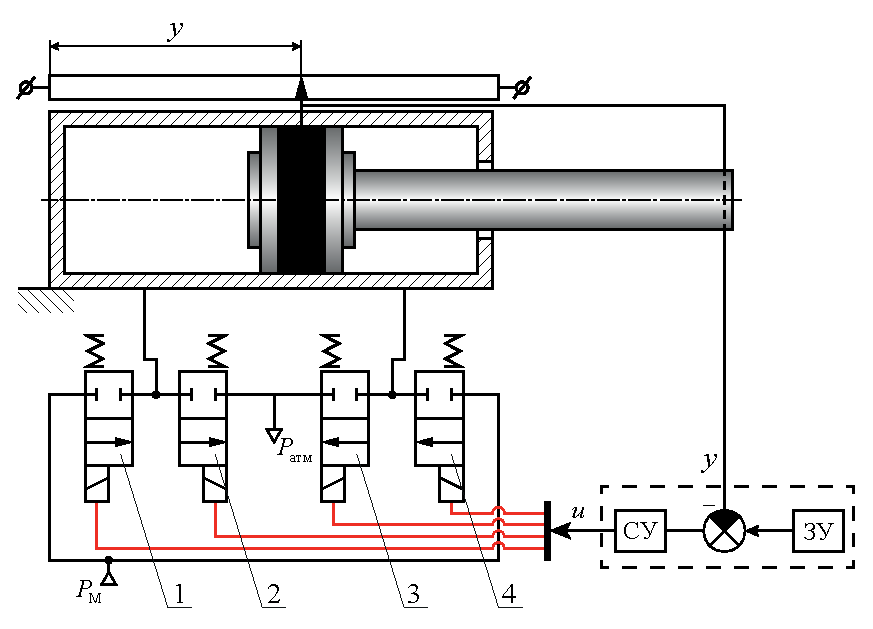
\includegraphics{part1/positioning_actuator_4_valve.eps}
    \caption{Структура позиционного пневмопривода с дискретными распределителями}\label{fig:pp_base_struct}
    \end{figure}


Несмотря на простоту, данная структура позволяет реализовать девять различных режимов
работы привода, включая режимы разгона, торможения и точного позиционирования. Это достигается исключительно за счет
различных комбинаций состояний распределителей без усложнения механической части системы. Таким образом, предложенная
конфигурация представляет собой оптимальный баланс между простотой реализации и функциональными возможностями позиционного пневмопривода.

\section{Выводы по главе 1}\label{sec:ch1/conclusion}

Анализ текущего состояния исследований в области позиционных пневмоприводов с
дискретными распределителями позволил выявить ряд существенных особенностей работы
и проблем, требующих решения:

\begin{enumerate}
	\item Установлено, что позиционные пневмоприводы с дискретными
	      распределителями представляют перспективное направление развития
	      пневмоавтоматики благодаря их низкой стоимости, высокой надежности
	      и простоте конструкции. При этом их эффективное функционирование
	      осложняется существенной нелинейностью динамических процессов,
	      обусловленной как физическими свойствами сжатого воздуха, так и
	      дискретным характером управляющих воздействий.

	\item Выявлено наличие трех противоречивых требований к характеристикам таких систем:
	      \begin{itemize}
		      \item обеспечение высокой точности позиционирования;
		      \item достижение требуемого быстродействия;
		      \item минимизация количества переключений распределителей.
	      \end{itemize}

	\item Обнаружены ключевые противоречия в оптимизации систем:
	      \begin{itemize}
		      \item повышение точности требует более частого переключения
		            распределителей, что приводит к ускоренному износу распределительной аппаратуры;
		      \item увеличение быстродействия негативно сказывается на
		            точности из-за возрастания динамических ошибок;
		      \item стремление к минимизации числа переключений
		            ограничивает возможности как точной коррекции положения, так и обеспечения требуемого быстродействия.
	      \end{itemize}

	\item Проведенный анализ существующих исследований показал
	      недостаточную проработку вопросов поиска компромисса между
	      частотой переключений распределителей и качеством позиционирования.
	      Существующие публикации, как правило, фокусируются на отдельных показателях качества без учета их взаимного влияния.

	\item Установлено, что оптимальным решением является структура с
	      четырьмя дискретными распределителями, обеспечивающая необходимую
	      функциональность системы позиционирования при сохранении простоты
	      технической реализации.

	\item Показано, что для эффективного решения задачи позиционирования
	      необходим интегративный подход к проектированию, учитывающий
	      взаимосвязанность процессов в пневматической, механической и
	      управляющей подсистемах.

	\item На основе проведенного анализа сформулирована необходимость
	      применения методов многокритериальной оптимизации, в частности,
	      построения фронта Парето, что позволит выявить предельно достижимые
	      характеристики системы.
\end{enumerate}

На основании этого, определены основные направления дальнейших исследований:
\begin{itemize}
	\item разработка уточненной математической модели пневмопривода,
	      учитывающей взаимосвязь термодинамических и механических процессов;
	\item синтез алгоритмов управления, обеспечивающих компромисс между
	      точностью позиционирования, быстродействием и интенсивностью переключений распределителей;
	\item построение и анализ фронта Парето для оптимизации параметров системы.
\end{itemize}

% 
\section{Анализ задачи торможения позиционного пневмопривода}\label{sec:ch1/sec4}

Одним из первопроходцев, начавший комплексное исследование задач торможения и позиционирования
РО ПП в заданной точке является А.А. Парой. В своей работе \cite*{парой:способы_торможения} автор статьи отмечает,
что более 40\%
современных промышленных роботов используют пневматические приводы, что объясняется их высокой надежностью и
низкой стоимостью. ПП применяются в качестве основного привода в промышленных роботах с
циклическим управлением и грузоподъемностью до 20~$\div$~30~\si{\kilogram}. Конструктивное решение таких роботов
предполагает использование длинноходовых пневмоцилиндров, которые позволяют реализовать режим
торможения в конце хода с помощью специальных тормозных устройств.

Согласно работе, существует два наиболее распространенных способа задания
тормозного усилия в выхлопной полости пневмопривода. Первый способ заключается в
резком уменьшении площади сечения выхлопного отверстия в определенной точке хода с
последующим поддержанием этой площади постоянной до конца хода. Второй способ предполагает
полное перекрытие площади сечения выхлопного отверстия на первом этапе торможения с последующим
открытием до определенной величины и уменьшением до нуля по определенному закону на втором этапе.
Автор статьи предлагает рассмотреть график, иллюстрирующий эти два режима (рисунок \cref*{fig:парой_режимы_торможения}).

\begin{figure}[h]
    \centerfloat
    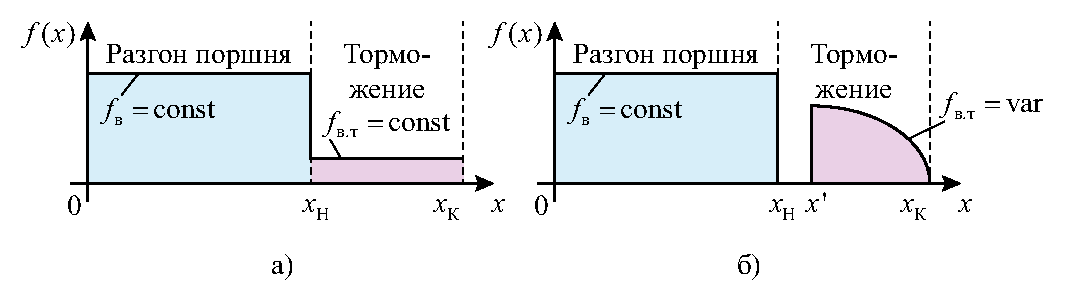
\includegraphics{paroy_brake_mode.eps}
    \caption{Режимы торможения}\label{fig:парой_режимы_торможения}
\end{figure}

Для проектирования тормозных устройств, использующих указанные способы, необходимо определить ряд
параметров, таких как координата начала торможения, площадь сечения выхлопного отверстия,
а также дополнительные координаты и закон изменения площади выхлопа для второго способа.
Автор статьи приводит математические модели, основанные на термодинамических и механических законах,
для расчета этих параметров.

Дальнейшей степенью развития стало комплексное рассмотрение способов торможения ПП в статье <<К вопросу выбора способа торможения
пневмоприводов с большими присоединенными массами>> Г.А. Крутикова, А.И. Кудрявцева и Л.А. Пекаря \cite*{крутиков:способы_торможения_12}
рассмотрено 12 схем торможения ПП, разделенные на 3 основные группы (I, II, III), показанные на рисунке \cref*{fig:эффективные_схемы_торможения_12}.

\begin{figure}[h]
    \centerfloat
    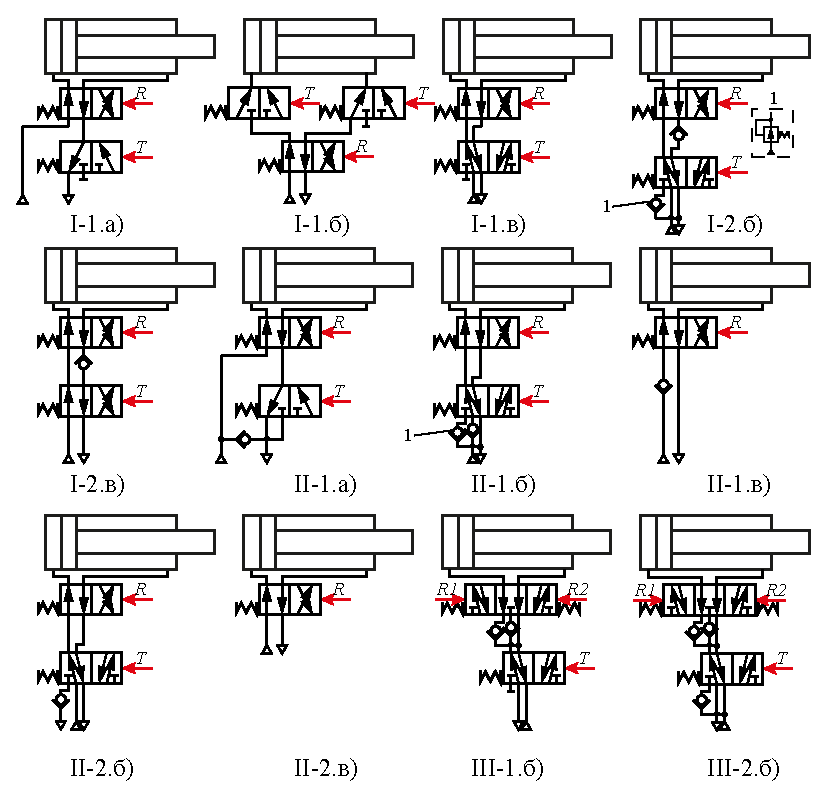
\includegraphics{kurtikob.eps}
    \caption{Эффективные схемы торможения ПП}\label{fig:эффективные_схемы_торможения_12}
\end{figure}

Отличительной особенностью этих схем является отсутствие регулируемых дросселей и емкостей ---
настройка оптимального режима торможения осуществляется только изменением тормозного пути.

Оценка эффективности каждой схемы осуществлялась по ряду ключевых критериев: время срабатывания ПП,
относительная масса сжатого воздуха, потребляемого за один цикл, осредненный за цикл КПД ПП, максимальное
ускорение при торможении, максимальная степень сжатия воздуха в тормозной полости, относительная стоимость
аппаратурной реализации и относительный тормозной путь. Для объективного сравнения каждой схеме была дана оценка в
баллах от 1 до 10 по каждому из показателей, причем максимальный балл присваивался схеме с наилучшим значением
параметра. Коэффициенты весомости различных критериев были определены экспертным методом в соответствии с
рекомендациями.

Наилучшие комплексные показатели качества продемонстрировали схемы III-2.б и III-1.б, которые, несмотря на
более высокую стоимость реализации, обладают лучшими энергетическими характеристиками, высоким быстродействием
и более плавным режимом торможения. Принципиальное отличие этих схем группы III заключается в том, что в них
используется не только вторая составляющая удельной работы сжатого воздуха (изотермическое расширение), но и его
потенциальная энергия, что существенно повышает КПД ПП.

Особого внимания заслуживает схема I-2.б с обратным клапаном, которая позволяет устранить недостатки схемы I-1.б
с высокими пиковыми ускорениями и отскоком поршня. Максимальное ускорение в этом случае снижается с 15,5~\si{\metre\per\square\second}
до 4,16~\si{\metre\per\square\second}, отскок минимален, а время срабатывания составляет 1,05~\si{\second}. Энергетические характеристики также улучшаются
за счет частичной рекуперации воздуха из тормозной полости.

Дальнейшее улучшение режима торможения обеспечивает модификация схемы I-2.б с установкой редукционного клапана вместо
обратного. Это позволяет реализовать практически равнозамедленный режим торможения с постоянным отрицательным
ускорением 1,38~\si{\metre\per\square\second}, полностью устраняет отскок поршня и обеспечивает предохранение тормозной полости от недопустимо
высоких давлений. Основными преимуществами такой схемы являются мягкий и плавный режим торможения с регулируемым
ускорением, экономное использование сжатого воздуха за счет рекуперации, высокое быстродействие и удобство настройки.

Таким образом, комплексная оценка и сравнение различных схем торможения ПП, проведенная авторами, позволила
выявить наиболее эффективные решения. В частности, схема I-2.б с редукционным клапаном демонстрирует оптимальное
сочетание высокого быстродействия, плавного режима торможения с заданным ускорением, экономного расхода сжатого
воздуха и защиты тормозной полости от чрезмерных давлений. Эта схема рекомендуется авторами для использования в качестве
внешнего тормозного устройства для ПП с большими инерционными нагрузками.

Итоговой компиляцией стала работа И.Б. Филипова \cite*{филипов:тормозные_устройства}. В своей монографии, автором подробно рассмотрены конструкции и
принципы построения тормозных устройств, применяемых преимущественно для торможения рабочих органов и звеньев машин
с пневмоприводами. Отмечается, что данные тормозные устройства весьма разнообразны по своему устройству и могут быть
механическими, пневматическими, гидравлическими, электрическими или комбинированными. Механические тормозные устройства
включают в себя пружинные, резиновые, эластомерные, инерционные и фрикционные конструкции, в то время как пневматические
могут быть напорными или вакуумными. Гидравлические тормозные устройства представляют собой устройства дроссельного
регулирования, а к электрическим относятся электромагнитные тормоза с сухим или жидким фрикционным наполнителем.
Кроме того, существуют комбинированные тормозные устройства, сочетающие в себе два или более типов перечисленных.

Автор классифицирует тормозные устройства по виду силовой характеристики или способу
преобразования кинетической энергии подвижных масс, схема классификации представлена на рисунке \cref*{fig:класс_схема_тормозных_устройств}.


\begin{figure}[h]
    \centerfloat
    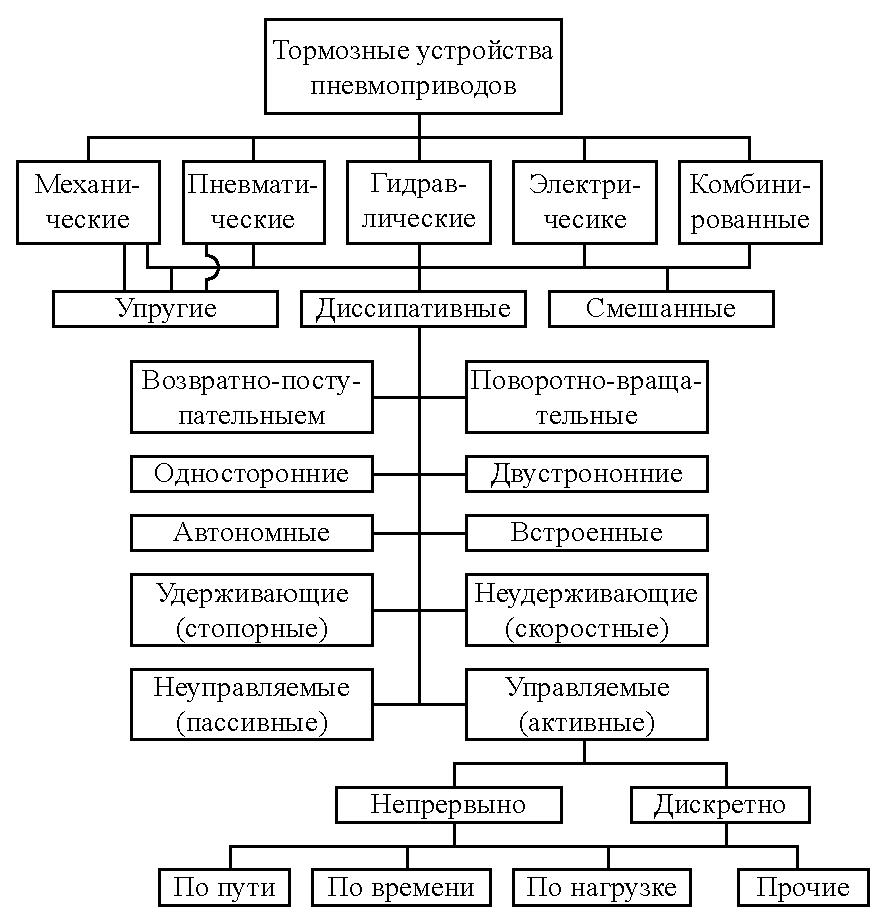
\includegraphics{class_scheme_break.eps}
    \caption{Классификационная схема тормозных устройств}\label{fig:класс_схема_тормозных_устройств}
\end{figure}


Выделяются устройства, создающие упругие,
диссипативные или упруго-диссипативные силы сопротивления. Большинство применяемых в настоящее
время тормозных устройств относятся к последнему типу, частично рассеивающих кинетическую энергию и
частично преобразующих ее в потенциальную. Также тормозные устройства могут быть возвратно-поступательного
или поворотно-вращательного типа движения выходного звена, а по виду действия - одностороннего или двустороннего.

Особое внимание в работе уделено автономным управляемым тормозным устройствам, которые могут быть унифицированы
и использованы для торможения движущихся масс механизмов с различными типами приводов. Их применение существенно
упрощает задачи компоновки и проектирования, а также эксплуатацию и обслуживание промышленного оборудования.
Автор приводит примеры конструктивного исполнения таких тормозных устройств, в том числе встроенных в пневмоцилиндры
для позиционирования выходного звена.

Помимо этого, в работе изложены основные требования к тормозным устройствам, такие как обеспечение заданного закона
торможения, ограничение ускорений, плавность торможения, высокая надежность и быстродействие, простота и компактность
конструкции, стабильность характеристик и другие. Для оценки эффективности применения тормозных устройств предлагается
использовать показатели, основанные на сравнении кинетической энергии, действующих сил, скоростей, ускорений и других
параметров движения выходного звена до и после их внедрения.

Так же, в данной монографии, автор подробно рассматривает особенности позиционных пневматических механизмов
с дискретным управлением, предназначенных для перемещения выходных звеньев или объектов из точки в точку по
заданной программе. Отмечается, что для таких механизмов основными требованиями являются обеспечение максимального
быстродействия и необходимой точности позиционирования при ограниченных динамических нагрузках.

Описывается конструкция и принцип работы разработанного позиционного ПП с одной дискретно управляемой полостью, представленного
на рисунке \cref*{fig:позиционный_пп_филипов}.

\begin{figure}[h]
    \centerfloat
    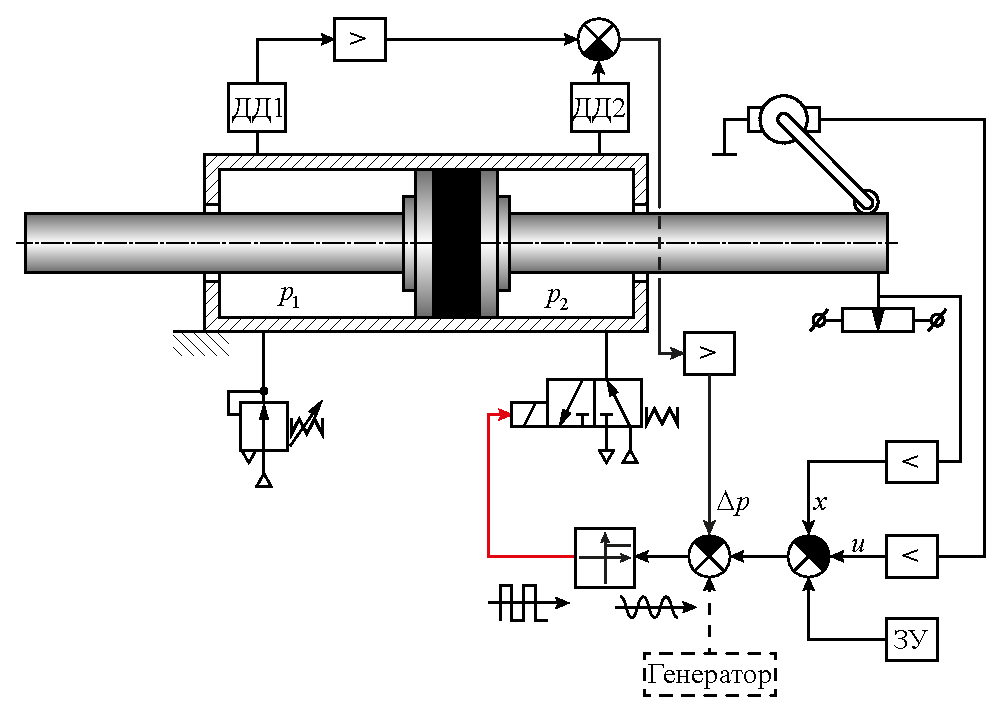
\includegraphics{philipov_positinon_act.eps}
    \caption{Схема дискретного пневмопозиционера}\label{fig:позиционный_пп_филипов}
\end{figure}

Его силовая часть состоит из пневмоцилиндра, в поршневой полости которого через редукционный клапан поддерживается
постоянное давление, а в штоковой полости давление регулируется трехлинейным двухпозиционным клапаном. Измерительная
часть включает датчики давления, тахогенератор и потенциометр для обратных связей по перемещению, скорости и перепаду
давления. Управление движением сводится к управлению торможением и позиционированием за счет переключения клапана,
соединяющего штоковую полость то с магистралью, то с атмосферой.

Автор отмечает, что вследствие колебания давления в штоковой полости уменьшается влияние зоны нечувствительности,
определяемой сухим трением. Приведены результаты исследований, показывающие, что частота переключения клапана определяется
его собственным временем запаздывания и мало зависит от других параметров, что позволяет избежать автоколебаний даже
в наиболее неблагоприятных точках позиционирования.

Дополнительные возможности открывает применение вибрационного сглаживания нелинейностей вынужденными колебаниями.
В этом случае при достижении сигналом рассогласования величины амплитуды гармонического воздействия клапан переходит
в режим постоянного переключения, поддерживая давление в управляемой полости таким, чтобы обеспечить торможение и точное
позиционирование. Преимуществом данного алгоритма является возможность задавать частоту вынужденных колебаний для
обеспечения необходимого качества переходного процесса и требуемого запаса устойчивости.

% 
\section{Анализ задач разгона и торможения в контексте системы управления}\label{sec:ch1/sec5}
В настоящее время, благодаря стремительному развитию микроэлектроники и её применению в различных
областях, стало возможным использование сложных алгоритмов управления. Эти достижения позволяют решать
вопросы, которые были исследованы ранее, при помощи разнообразных алгоритмов управления.

Однако применение алгоритмов управления, предназначенных для непрерывных систем, к системам с
дискретными элементами может быть затруднительным или даже невозможным. Для использования
ПИД-регулятора исследователи применяют различные преобразователи и модуляции сигнала. Например,
широко распространено использование широтно-импульсной модуляции (ШИМ) в сочетании с ПИД.

Аналогично, инженеры используют разнообразные интеллектуальные алгоритмы управления на основе
нейросетей или нечёткой логики. Также особую популярность получило управление в скользящих режимах,
которое зарекомендовало себя в управлении электроприводом. Это связано с тем, что модель представляет
собой дискретную систему.

\subsection{Исследование управления с использованием ШИМ}\label{subsec:ch1/sec5/subsec1}

В работе \cite*{pwm:Varseveld} подробно рассмотрена разработка системы позиционного ПП, схема которого представлена на
рисунке \ref*{fig:позиционный_пп_pwm}, с использованием недорогих
дискретных распределителей с электромагнитным управлением, вместо дорогостоящих пропорциональных. Особое внимание уделено
проектированию системы управления, обеспечивающей высокое быстродействие и точность позиционирования.

\begin{figure}[htpb]
    \centerfloat
    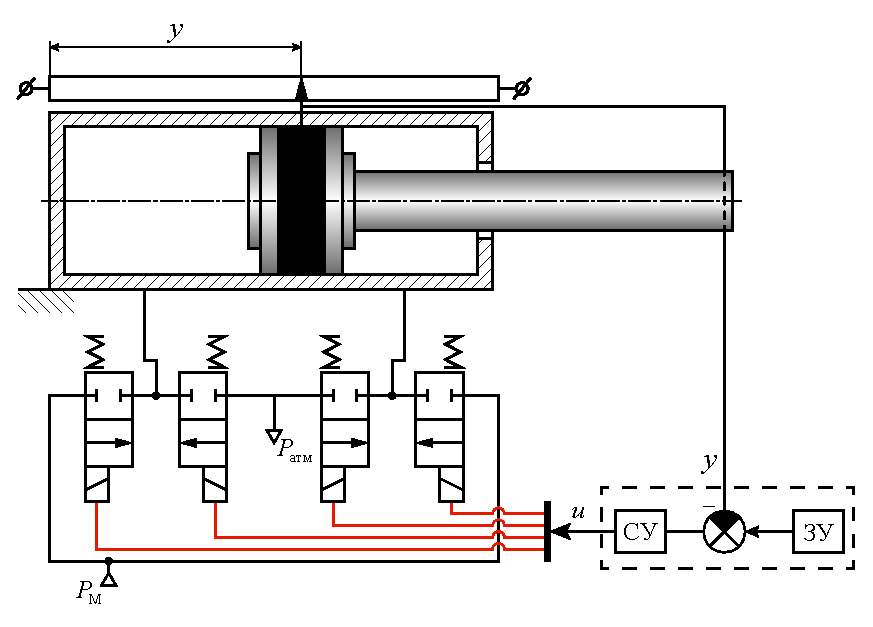
\includegraphics{positioning_actuator_pwm_ov.eps}
    \caption{Схема позиционного ПП с дискретными распределителями}\label{fig:позиционный_пп_pwm}
\end{figure}

Авторами предложен новый алгоритм с использованием широтно-импульсной модуляции (ШИМ) для управления распределителями, позволяющий
получить практически симметричную и линейную характеристику скорости РО ПП в зависимости от управляющего сигнала.
Это достигается за счет согласованного управления магистральными и выхлопными распределителями, что компенсирует асимметрию,
вызванную разницей активных площадей поршня в поршневой и штоковой полостях. Экспериментальные исследования подтвердили высокую линейность и
симметрию полученной характеристики.

На основе экспериментальных данных авторами синтезирована линейная авторегрессионная модель ПП.
Анализ модели показал, что демпфирование системы существенно зависит от положения поршня, достигая минимума в
центральной части хода. Это объясняется наличием сухого кулоновского трения.

Для компенсации влияния трения в систему управления введен ПИД-регулятор с дополнительной компенсацией
трения и интегральной составляющей ограниченной с двух сторон. Применение этих мер позволило существенно уменьшить статическую
ошибку позиционирования.

В ходе экспериментальных исследований авторам удалось достичь высокого быстродействия системы управления --
время нарастания составило всего 180~\si{\milli\second}. При этом статическая ошибка позиционирования не превышала 0,21~
\si{\milli\metre},
что сопоставимо с результатами, полученными другими исследователями
\cite*{Varseveld:article1,Varseveld:article2,Varseveld:article3,Surgenor1997ContinuousSM},
использовавшими более дорогостоящие
пропорциональные распределители. Кроме того, система продемонстрировала инвариантность к шестикратному изменению
инерционной нагрузки. Авторы также показали возможность точного отслеживания $S$-образных траекторий с ошибкой не
более 2~\si{\milli\metre}.

Статья \cite*{Shiee} посвящена сравнительному анализу различных схем ШИМ для улучшения позиционирования ПП. Авторы рассматривают пять
основных ШИМ-схем представленных на рисунке \ref*{fig:схемы_шим}.

\begin{figure}[ht]
    \centerfloat{
        \subcaptionbox[List-of-Figures entry]{\label{fig:схемы_шим-1}}{
            \begin{tikzpicture}
                \begin{axis}[
                        width = 8cm,
                        height = 5cm,
                        xmin=-100, xmax=100,
                        ymin=0, ymax=100,
                        xlabel={Сигнал, \%},
                        ylabel={Ширина ШИМ, \%},
                        grid=major,
                        extra tick style={grid=none, draw opacity=0},
                        tick style={line width=0.75pt},
                        axis line style={line width=1pt},
                    ]
                    \addplot[black, mark=none, line width=0.75pt] coordinates {
                            (-100, 0)
                            (100, 100)
                        };
                    \addplot[black, mark=none, line width=0.75pt, dashed] coordinates {
                            (-100, 100)
                            (100, 0)
                        };
                    %add legend
                    \addlegendentry{Расп. 1}
                    \addlegendentry{Расп. 2}


                \end{axis}
            \end{tikzpicture}
        }
        \hfil
        \subcaptionbox[]{\label{fig:схемы_шим-2}}{
            \begin{tikzpicture}
                \begin{axis}[
                        width = 8cm,
                        height = 5cm,
                        xmin=-100, xmax=100,
                        ymin=0, ymax=100,
                        xlabel={Сигнал, \%},
                        ylabel={Ширина ШИМ, \%},
                        grid=major,
                        extra tick style={grid=none, draw opacity=0},
                        tick style={line width=0.75pt},
                        axis line style={line width=1pt},
                    ]
                    \addplot[black, mark=none, line width=0.75pt] coordinates {
                            (-100, 10)
                            (-80, 10)
                            (80, 80)
                            (100, 100)
                        };
                    \addplot[black, mark=none, line width=0.75pt, dashed] coordinates {
                            (-100, 100)
                            (-80, 80)
                            (80, 10)
                            (100, 10)
                        };
                    %add legend
                    \addlegendentry{Расп. 1}
                    \addlegendentry{Расп. 2}


                \end{axis}
            \end{tikzpicture}
        }
        \vfil
        \subcaptionbox[]{\label{fig:схемы_шим-3}}{
            \begin{tikzpicture}
                \begin{axis}[
                        width = 8cm,
                        height = 5cm,
                        xmin=-100, xmax=100,
                        ymin=0, ymax=100,
                        xlabel={Сигнал, \%},
                        ylabel={Ширина ШИМ, \%},
                        grid=major,
                        extra tick style={grid=none, draw opacity=0},
                        tick style={line width=0.75pt},
                        axis line style={line width=1pt},
                    ]
                    \addplot[black, mark=none, line width=0.75pt] coordinates {
                            (-100, 20)
                            (-70, 20)
                            (70, 80)
                            (100, 80)
                        };
                    \addplot[black, mark=none, line width=0.75pt,dashed] coordinates {
                            (-100, 80)
                            (-70, 80)
                            (70, 20)
                            (100, 20)
                        };
                    %add legend
                    \addlegendentry{Расп. 1}
                    \addlegendentry{Расп. 2}
                \end{axis}
            \end{tikzpicture}
        }
        \hfil
        \subcaptionbox[]{\label{fig:схемы_шим-4}}{
            \begin{tikzpicture}
                \begin{axis}[
                        width = 8cm,
                        height = 5cm,
                        xmin=-100, xmax=100,
                        ymin=0, ymax=100,
                        xlabel={Сигнал, \%},
                        ylabel={Ширина ШИМ, \%},
                        grid=major,
                        extra tick style={grid=none, draw opacity=0},
                        tick style={line width=0.75pt},
                        axis line style={line width=1pt},
                    ]
                    \addplot[black, mark=none, line width=0.75pt, ] coordinates {
                            (-100, 20)
                            (0, 20)
                            (100, 80)
                        };
                    \addplot[black, mark=none, line width=0.75pt, dashed] coordinates {
                            (-100, 80)
                            (0, 20)
                            (100, 20)
                        };
                    %add legend
                    \addlegendentry{Расп. 1}
                    \addlegendentry{Расп. 2}
                \end{axis}
            \end{tikzpicture}
        }
        \vfil    \subcaptionbox[]{\label{fig:схемы_шим-5}}{
            \begin{tikzpicture}
                \begin{axis}[
                        width = 8cm,
                        height = 5cm,
                        xmin=-100, xmax=100,
                        ymin=0, ymax=100,
                        xlabel={Сигнал, \%},
                        ylabel={Ширина ШИМ, \%},
                        grid=major,
                        extra tick style={grid=none, draw opacity=0},
                        tick style={line width=0.75pt},
                        axis line style={line width=1pt},
                    ]
                    \addplot[black, mark=none, line width=0.75pt, ] coordinates {
                            (-100, 20)
                            (0, 80)
                            (100, 80)
                        };
                    \addplot[black, mark=none, line width=0.75pt, dashed] coordinates {
                            (-100, 80)
                            (0, 80)
                            (100, 20)
                        };
                    %add legend
                    \addlegendentry{Расп. 1}
                    \addlegendentry{Расп. 2}
                \end{axis}
            \end{tikzpicture}
        }
    }
    \caption{Схемы ШИМ}\label{fig:схемы_шим}
\end{figure}

Схема \cref*{fig:схемы_шим-1} не учитывает динамику включения/выключения распределителей, что приводит к нелинейностям при
крайних значениях входного сигнала. Схема \cref*{fig:схемы_шим-2} учитывает только динамику включения распределителей и добавляет точку перегиба,
чтобы минимизировать ширину импульса ниже определенного значения. Схема \cref*{fig:схемы_шим-3} учитывает как задержку включения, так и
задержку выключения распределителей, вводя два пограничных значения для ширины импульса. Схема \cref*{fig:схемы_шим-4} является модифицированным
вариантом схемы \cref*{fig:схемы_шим-1}, учитывающим задержки клапанов, и обеспечивает меньшую сумму коэффициентов заполнения сигнала поступающего на распределитель,
особенно вблизи нулевого входного сигнала. Схема \cref*{fig:схемы_шим-5} представляет собой модификацию схемы \cref*{fig:схемы_шим-3} с
учетом задержек включения
и выключения клапанов, давая большую суммарную ширину импульса вблизи нулевого входа.

Авторы провели ряд экспериментов со ступенчатыми и гармоническими входными воздействиями, чтобы изучить характеристики
различных ШИМ-схем. По характеристикам позиционирования при ступенчатом входе, схема \cref*{fig:схемы_шим-1} показала наименьшее время
нарастания, но большую статическую ошибку позиционирования, схема \cref*{fig:схемы_шим-4} продемонстрировала наименьшее перерегулирование,
но худшую ошибку, а схема \cref*{fig:схемы_шим-5} имела самое большое время нарастания и ошибку.
При отслеживании гармонического сигнала, первые три схемы показали близкие результаты по среднеквадратичной
ошибке, в то время как схемы \cref*{fig:схемы_шим-4} и \cref*{fig:схемы_шим-5} имели большую ошибку слежения. Эксперименты с увеличением нагрузки показали,
что схема \cref*{fig:схемы_шим-4}
оказалась наименее устойчивой к увеличению инерционной нагрузки, а схема \cref*{fig:схемы_шим-5}, имеющая высокое рабочее давление,
продемонстрировала наибольшую
устойчивость.

Чтобы компенсировать влияние различий в эффективных площадях, авторы предложили модифицированные версии каждой ШИМ-схемы.
Модификация заключается в сдвиге диаграмм ШИМ-схем с целью достижения нулевой выходной силы при нулевом входном сигнале.

Экспериментальные результаты при ступенчатом входном воздействии продемонстрировали, что модифицированные ШИМ-схемы, особенно для схем \cref*{fig:схемы_шим-1},
\cref*{fig:схемы_шим-2}, \cref*{fig:схемы_шим-3} и \cref*{fig:схемы_шим-5}, обеспечивают значительное улучшение характеристик позиционирования,
в частности, снижение статической ошибки позиционирования. Это связано с тем, что при высоких рабочих давлениях различия в эффективных площадях поршня
становятся более значимыми, и предложенные модификации эффективно компенсируют этот эффект.

В следующей статье \cite*{Tran:pwm} авторами представлен модифицированный метод позиционного управления
ПП с использованием четырех дискретных электромагнитных распределителей, схема ПП аналогична схеме
представленной на рисунке \cref*{fig:позиционный_пп_pwm}.

Первоначально в работе проведен анализ алгоритма, разработанного другим автором \cite*{Truong}
в 2007 году. Установлено, что данный алгоритм демонстрирует существенное
перерегулирование при задании малых положений поршня, что обусловливает необходимость
дальнейшего совершенствования методов управления.

С целью повышения качества позиционирования авторами была предложена модификация
алгоритма. Ключевым аспектом модификации стало разделение диапазона задаваемых
положений на две области: малые положения $(x_d \leqslant \text{50}~\si{\milli\metre})$
и большие положения $(x_d > \text{50}~\si{\milli\metre})$.
Для каждой области авторами разработаны индивидуальные законы управления с использованием
семи различных режимов работы четырех электромагнитных распределителей в сочетании с ШИМ.

Для диапазона малых положений при значительной ошибке позиционирования
$e \leqslant -\alpha$ авторами
введен новый режим $M_6$, предполагающий одновременное открытие двух распределителей, что обеспечивало
плавное низкоскоростное движение. В области промежуточных ошибок
$-\alpha < e < -\beta$ применялся режим
$M_2$ с импульсным открытием одного из распределителей, способствующий быстрому замедлению движения и
устранению перерегулирования.

Для диапазона больших положений авторами модифицированы режимы $M_2$ и $M_2$ контроллера
посредством организации поочередного импульсного открытия распределителей. Данный подход позволял
плавно замедлять движение поршня.

Экспериментальные исследования подтвердили, что модифицированный алгоритм обеспечивает
существенное улучшение качества позиционного управления по сравнению с исходным алгоритмом,
особенно при отработке малых положений. Более того, при частотах задающего воздействия
до \num{0.1}~\si{\hertz} модифицированный алгоритм продемонстрировал сопоставимые или превосходящие
характеристики относительно алгоритма для ПП с пропорциональными
распределителями. Однако при более высоких частотах (например, \num{0.5}~\si{\hertz}) характеристики модифицированного
алгоритма значительно ухудшались, что связано с ограниченной скоростью переключения
используемых распределителей.

Таким образом, результаты проведенного исследования свидетельствуют о том, что предложенный
модифицированный алгоритм позволяет существенно повысить качество позиционного управления
пневматическим приводом с дискретными распределителями при низких и средних частотах задающего
воздействия по сравнению с ранее разработанными решениями.

В следующей работе \cite*{AHN2005683} так же представлен подход к разработке системы управления ПП
с использованием дискретных электромагнитных распределителей вместо традиционных пропорциональных распределителей.
Авторы предлагают модифицированный алгоритм ШИМ для точного позиционного управления
ПП при помощи этих дискретных распределителей.

Центральным элементом разработанной системы управления является трехконтурная схема, представленная на рисунке
\cref*{fig:mpwm_lvqnn},
\begin{figure}[htpb]
    \centerfloat
    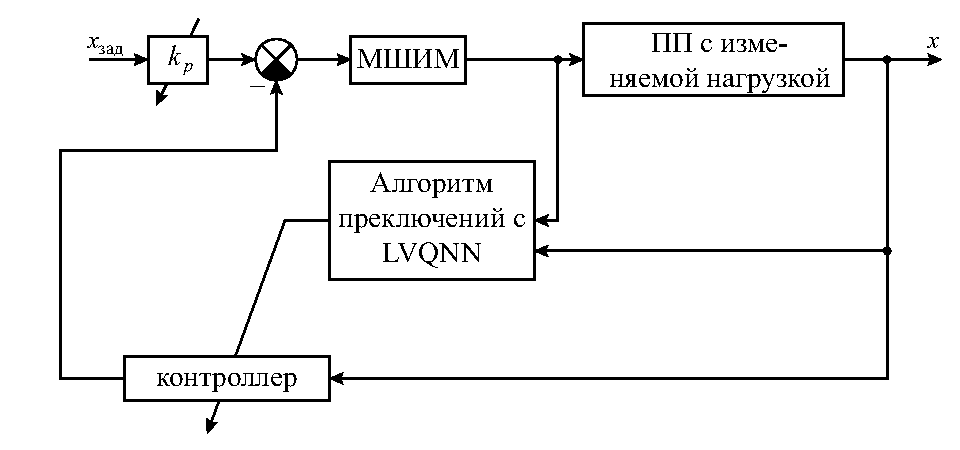
\includegraphics{mpwm_lvqnn.eps}
    \caption{Структурная схема системы управления с МШИМ и LVQNN}\label{fig:mpwm_lvqnn}
\end{figure}
с обратной связью по положению, скорости и ускорению. Такая структура обеспечивает высокое быстродействие и
точность позиционирования. Для адаптации параметров регулятора к изменяющимся внешним нагрузкам авторы применяют
нейронную сеть на основе векторного квантования (LVQNN). Данная интеллектуальная система классификации нагрузки
динамически подстраивает коэффициенты регулятора, компенсируя влияние возмущающих воздействий.

Проведённые экспериментальные исследования подтвердили, что предложенный алгоритм МШИМ обеспечивает точность позиционирования
в пределах \num{0.2}~\si{\milli\metre}, что существенно превосходит результаты стандартного ШИМ-алгоритма (ошибка около \num{1.75}~\si{\milli\metre}). Применение
LVQNN и адаптивной настройки параметров регулятора позволило эффективно компенсировать влияние изменяющейся внешней нагрузки и
добиться высокой стабильности системы управления.

Таким образом, ключевыми элементами разработанной системы управления являются алгоритм МШИМ,
трёхконтурная схема регулирования с обратной связью, а также интеллектуальная система адаптации параметров
регулятора на основе LVQNN. Полученные результаты демонстрируют высокую эффективность предложенных методов для точного
позиционного управления пневматическим пневмоприводом в условиях изменяющихся внешних нагрузок.


%%%%%%%%%%%%%%%%%%%%%%%%%%%%%%%%%%%%%%%%%%%%%%%%%%%%%%%%%%%%%%%%%%%%%%%%%%%%%%%%%%%%%%%%%%%%%%%%%%%%%%%%%%%%%%%%%%%%%%%%%%%%
%%%%%%%%%%%%%%%%%%%%%%%%%%%%%%%%%%%%%%%%%%%%%%%%%%%%%%%%%%%%%%%%%%%%%%%%%%%%%%%%%%%%%%%%%%%%%%%%%%%%%%%%%%%%%%%%%%%%%%%%%%%%
%%%%%%%%%%%%%%%%%%%%%%%%%%%%%%%%%%%%%%%%%%%%%%%%%%%%%%%%%%%%%%%%%%%%%%%%%%%%%%%%%%%%%%%%%%%%%%%%%%%%%%%%%%%%%%%%%%%%%%%%%%%%

\subsection{Исследование управления в скользящих режимах}\label{subsec:ch1/sec5/subsec2}

Управление в скользящих режимах \cite*{utkin2017sliding} -- это класс нелинейных методов управления, которые делают систему управления разрывной.
Процесс проектирования делится на два этапа: выбор поверхностей переключения для желаемого режима движения и синтез разрывного
управления для движения системы по этим поверхностям.

Движение системы по поверхностям переключения обладает рядом преимуществ: снижение порядка системы, инвариантность
к параметрическим и внешним возмущениям. Для описания движения используются специальные математические методы, такие
как регуляризация и метод эквивалентного управления.

Управление в скользящих режимах эффективно решает задачи управления сложными нелинейными динамическими объектами в
условиях неопределённости и широко применяется в электроприводах, робототехнике и системах автоматического управления.
Поскольку позиционный ПП с дискретными распределителями представляет из себя дискретную систему с релейным
управлением, то предостваляется воозможным использовать управление в скользящих режимах в ПП.

%%%%%%%%%%%%%%%%%%%%%%%%%%%%%%%%%%%%%%%%%%%%%%%%%%%%%%%%%%%%%%%%%%%%%%%%%%%%%%%%%%%%%%%%%%%%%%%%%%%%%%%%%%%%%%%%%%%%%%%%%%%%


В статье \cite*{Elsayed} рассматривается исследование, посвящённое управлению положением РО ПП
с использованием дискретных распределителей.

Авторы предлагают использование алгоритма управления скользящим режимом с коррекцией ошибки регулирования (SMCE), который использует
ШИМ для управления распределителями.

Для управления движением пневматического цилиндра авторы используют только три режима работы
четырёх распределителей, представленные ниже:
\begin{enumerate}
    \item Режим 1 -- выдвижение штока;
    \item Режим 2 -- задвижение штока;
    \item Режим 3 -- удержание положения штока;
\end{enumerate}

С целью оптимизации параметров SMCE и ПИД-регулятора была разработана модель в Simulink.
Экспериментальные исследования проводились на стенде ПП.

Результаты моделирования и экспериментов показывают, что SMCE обеспечивает более высокую точность
позиционирования, меньшее время установления и меньший выброс по сравнению с традиционным ПИД-регулятором.
Для гармонического входного сигнала среднеквадратичная ошибка при использовании SMCE составляет \num{0.22}~\si{\milli\metre}, а
для ПИД -- \num{0.69}~\si{\milli\metre}. Максимальная абсолютная ошибка для SMCE составляет \num{0.66}~\si{\milli\metre},
а для ПИД -- \num{1.46}~\si{\milli\metre}. Таким образом,
предложенный метод SMCE показал своё превосходство над ПИД-регулятором при управлении положением РО ПП.
%%%%%%%%%%%%%%%%%%%%%%%%%%%%%%%%%%%%%%%%%%%%%%%%%%%%%%%%%%%%%%%%%%%%%%%%%%%%%%%%%%%%%%%%%%%%%%%%%%%%%%%%%%%%%%%%%%%%%%%%%%%%

Статья \cite*{Hodgson:article1} аналогично посвящена разработке алгоритма управления в скользящих режимах
для регулирования ПП
с четырмя дискретными распределителями.

Ключевым отличием от предыдущих работ является расширение числа доступных дискретных режимов управления
с трех до семи.

В основе контроллера лежит скользящая поверхность $s$, которая определяется как функция ошибки позиционирования $e$,
её производной и второй производной. Авторы вводят семь возможных режимов переключения распределителей $(M_1 \div M_7)$,
выбор которых производится в зависимости от текущего значения $s$ и eё производной. Диаграмма переходов
представлена на рисунке.

\begin{figure}[ht]
    \centerfloat{
        \begin{tikzpicture}[auto]
            \usetikzlibrary {matrix,positioning,shapes.misc,arrows,shapes.geometric,graphs,backgrounds,arrows.meta}
            \tikzstyle{main_block} = [rectangle, rounded corners=0.5cm, draw, text centered, minimum height=4em, line width=1pt, text width=6em]
            \tikzstyle{text_block} = [rectangle, rounded corners=0.25cm, text centered, fill=white]
            \tikzstyle{cond_block} = [diamond, text centered, draw, text centered, line width = 1pt]
            \tikzstyle{arr} = [-triangle 45, line width=1pt]
            \tikzstyle{line} = [-, line width=1pt]
            % \tikzstyle{dashed} = [-triangle 45, line width=1pt, dashed]
            \matrix [column sep=3mm, row sep=7mm]
            {
                                                                              &
                                                                              &
                \node[main_block] (M7) {$M_7$\\$P_1$ -- оп.\\$P_2$ -- нап.};    \\
                %
                \node[text_block] (t1_0) {$\beta$};                           &
                \node[text_block] (t1_1) {$s > \beta$};                       &
                \node[text_block] (t1_2) {$s > \beta$};                       &
                \node[text_block] (t1_3) {$s > \beta$};                         \\
                %
                                                                              &
                \node[main_block] (M5) {$M_5$\\$P_1$ -- зап.\\$P_2$ -- нап.}; &
                \node[cond_block] (C1) {$E_1 > 1$};                           &
                \node[main_block] (M3) {$M_3$\\$P_1$ -- оп.\\$P_2$ -- зап.};    \\
                %
                \node[text_block] (t2_0) {$\epsilon$};                        &
                \node[text_block] (t2_1) {$s < \epsilon$};                    &
                \node[text_block] (t2_2) {$s > \epsilon$};                    &
                \node[text_block] (t2_3) {$s < \epsilon$};                      \\
                %
                                                                              &
                                                                              &
                \node[main_block] (M1) {$M_1$\\$P_1$ -- зап.\\$P_2$ -- зап.};   \\
                %
                \node[text_block] (t3_0) {$-\epsilon$};                       &
                \node[text_block] (t3_1) {$s > -\epsilon$};                   &
                \node[text_block] (t3_2) {$s < -\epsilon$};                   &
                \node[text_block] (t3_3) {$s > -\epsilon$};                     \\
                %
                                                                              &
                \node[main_block] (M2) {$M_2$\\$P_1$ -- нап.\\$P_2$ -- зап.}; &
                \node[cond_block] (C2) {$E_1 > 1$};                           &
                \node[main_block] (M4) {$M_4$\\$P_1$ -- зап.\\$P_2$ -- оп.};    \\
                %
                \node[text_block] (t4_0) {$-\beta$};                          &
                \node[text_block] (t4_1) {$s < -\beta$};                      &
                \node[text_block] (t4_2) {$s > -\beta$};                      &
                \node[text_block] (t4_3) {$s < -\beta$};                        \\
                %
                                                                              &
                                                                              &
                \node[main_block] (M6) {$M_6$\\$P_1$ -- нап.\\$P_2$ -- оп.};    \\
                %%%%%%%%%%%%%%%%%%%%%%%%%%%%%%%%%%%%%%%%%%%%%%%%%%%%%%%%%%%%%%%%%%%%
            };
            \begin{scope}[on background layer]
                \draw[arr] (M7.south) -- (C1);
                \draw[line] (M5.north) -- (t1_1);
                \draw[arr] (t1_1.north) to [out=90,in=180]  (M7.west);
                \draw[line] (M3.north) -- (t1_3);
                \draw[arr] (t1_3.north) to [out=90,in=0] (M7.east);

                \draw[arr] ([xshift=1cm]M5.north) to [out=90,in=90] node[below] {$\tau$} (C1.north);
                \draw[arr] ([xshift=-1cm]M3.north) to [out=90,in=90] node[below] {$\tau$} (C1.north);
                %%%%%%%%%%%%%%%%%%%%%%%%%%%%%%%%%%%%%%%%%%%%%%%%%%%%%%%%%%%%%
                \draw[line, loosely dashed] (t1_0.east) -- ([xshift=3cm]t1_3.west);
                \draw[line, loosely dashed] (t2_0.east) -- ([xshift=3cm]t2_3.west);
                \draw[line, loosely dashed] (t3_0.east) -- ([xshift=3.4cm]t3_3.west);
                \draw[line, loosely dashed] (t4_0.east) -- ([xshift=3.4cm]t4_3.west);

                \draw[line] (M5.south) -- (t2_1.north);
                \draw[line] (M3.south) -- (t2_3.north);
                %%%%%%%%%%%%%%%%%%%%%%%%%%%%%%%%%%%%%%%%%%%%%%%%%%%%%%%%%%%%%
                \draw[arr] (C1.west) -- (M5.east);
                \draw[arr] (C1.east) -- (M3.west);

                \draw[arr] (t2_1.south) to [out=-90,in=180]  (M1.west);
                \draw[arr] (t2_3.south) to [out=-90,in=0] (M1.east);

                \draw[arr] (M1.north) -- (C1.south);
                %%%%%%%%%%%%%%%%%%%%%%%%%%%%%%%%%%%%%%%%%%%%%%%%%%%%%%%%%%%%%

                \draw[arr] (M1.south) -- (C2);
                \draw[line] (M2.north) -- (t3_1);
                \draw[arr] (t3_1.north) to [out=90,in=180]  (M1.west);
                \draw[line] (M4.north) -- (t3_3);
                \draw[arr] (t3_3.north) to [out=90,in=0] (M1.east);

                \draw[arr] ([xshift=1cm]M2.south) to [out=-90,in=-90] node[above] {$\tau$} (C2.south);
                \draw[arr] ([xshift=-1cm]M4.south) to [out=-90,in=-90] node[above] {$\tau$} (C2.south);

                \draw[arr] (M6.north) -- (C2.south);

                \draw[line] (t4_1.north) --  (M2.south);
                \draw[line] (t4_3.north) --  (M4.south);

                \draw[arr] (t4_1.south) to [out=-90,in=180]  (M6.west);
                \draw[arr] (t4_3.south) to [out=-90,in=0] (M6.east);

                \draw[arr] (C2.west) -- (M2.east);
                \draw[arr] (C2.east) -- (M4.west);

                \draw[arr] ([xshift=-6cm]M6.south) -- node {$s$} ([xshift=-6cm]M7.north);

                % %%%%%%%%%%%%%%%%%%%%%%%%%%%%%%%%%%%%%%%%%%%%%%%%%%%%%%%%%%%%%
                % \draw[line, loosely dashed] (t1_0.east) -- ([xshift=3cm]t1_3.west);
                % \draw[line, loosely dashed] (t2_0.east) -- ([xshift=3cm]t2_3.west);
                % \draw[line, loosely dashed] (t3_0.east) -- ([xshift=3.4cm]t3_3.west);
                % \draw[line, loosely dashed] (t4_0.east) -- ([xshift=3.4cm]t4_3.west);
            \end{scope}
        \end{tikzpicture}
    }
    \caption{Диаграмма переключения режимов }\label{fig:actuators_scheme}
\end{figure}

Режимы $M_7$ и $M_6$ применяются при больших по модулю значениях $s$ для обеспечения максимальных ускорений в положительном и
отрицательном направлениях соответственно. Эти режимы позволяют быстро сократить большие ошибки позиционирования.

Режимы $M_2, M_3, M_4$ и $M_5$ используются при малых ошибках позиционирования $(\lvert s \rvert < \beta)$. Их применение позволяет снизить частоту
переключений распределителей, что способствует увеличению срока службы пневматической системы.

Для выбора оптимального режима в области малых ошибок авторы вводят дополнительные критерии, основанные на разности давлений
в камерах пневмопривода. Это позволяет определить режим, обеспечивающий максимальное ускорение при минимальном переключении
распределителей. Кроме того, вводится параметр $\tau$, задающий минимальное время между переключениями в этой области, что также
способствует снижению частоты переключений распределителей.

Теоретический анализ показывает, что при достаточно больших значениях параметров распределителей, предложенный алгоритм
обеспечивает асимптотическую устойчивость замкнутой системы. Результаты моделирования и экспериментальных исследований подтверждают,
что семирежимный скользящий контроллер демонстрирует улучшение точности позиционирования и значительное снижение переключений соленоидных
распределителей по сравнению с трехрежимным аналогом.

Таким образом, данная работа предлагает эффективное решение для управления пневматическими приводами с дискретными входами, обеспечивая
высокую точность позиционирования при сокращении нагрузки на исполнительные механизмы.

%%%%%%%%%%%%%%%%%%%%%%%%%%%%%%%%%%%%%%%%%%%%%%%%%%%%%%%%%%%%%%%%%%%%%%%%%%%%%%%%%%%%%%%%%%%%%%%%%%%%%%%%%%%%%%%%%%%%%%%%%%%%

Аналогично, в статье \cite*{Zhonglin} рассматривается разработка и проверка алгоритма управления в скользящем режиме с
использованием ШИМ для систем позиционирования в ПП. Этот алгоритм был так же применён к ПП с четырьмя дискретными распределителями.

Основная цель исследования заключалась в снижении ошибок позиционирования и повышении точности слежения. В статье подробно рассматриваются существующие подходы к управлению в ПП системах.

Разработанный алгоритм основан на использовании семи режимов переключения распределителей. В отличие от традиционных методов,
использующих высокое или низкое напряжение в одном периоде ШИМ, предложенная методика применяет два режима переключения за один период,
что улучшает производительность, комбинируя управление фазами ШИМ.

Статья подробно описывает процесс разработки алгоритма управления с использованием скользящего режима.
Он начинается с математической модели и заканчивается настройкой параметров и верификацией системы на платформе FPGA.
Использование FPGA в электропневматических системах является инновационным подходом. Авторы продемонстрировали эффективность
предложенного алгоритма как в математической модели, так и в экспериментальных условиях.

Экспериментальная часть включает настройку аппаратной части системы и платформы FPGA, а также тестирование на реальной установке.
Результаты подтвердили высокую точность и надёжность предложенного метода по сравнению с традиционными подходами.

Авторы подытоживают, что предложенный алгоритм обеспечивает высокую точность и устройчивость управления.
Предложенный алгоритм позволил уменьшить статическую ошибку позиционирования с \num{2.5}~\si{\milli\metre} до \num{0.8}~\si{\milli\metre},
что составляет снижение ошибки на \num{68}\%.
В свою очередь, точность позиционирования при математическом моделировании достигла \num{98.5}\% по сравнению с \num{91.2}\% при
использовании традиционных методов.

Кроме того, время отклика системы сократилось на 33\%, обеспечивая более высокое быстродействие. В
эксперименте отклонение при повторяющихся циклах позиционирования не превышало \num{1.2}~\si{\milli\metre}, тогда как
у традиционного алгоритма с ШИМ, это значение было в среднем \num{3.7}~\si{\milli\metre}.

\subsection{Исследование управления c применением интеллектуальных алгоритмов}\label{subsec:ch1/sec5/subsec3}

Интеллектуальные алгоритмы представляют из себя класс методов, основанных на применнении ИИ и МО для решения задач управления, в
которых требуется адаптация, обучаемость и предсказательность поведения в процессе функционирования. В отличии от классических методов,
интелектуальные методы способны анализировать поступающие данные, обучаться на их основе и принимать решения, основываясь на полученном или
накопленном опыте.

Можно выделить основные аспекты, которыми владееют интеллектуальные алгоритмы:
\begin{enumerate}
    \item способность к адаптации к изменяющимся условиям;
    \item способность к обучению на основе данных;
    \item способность к принятию решений на основе полученной информации;
    \item способность поиска оптимальных решений в условиях неопределённости.
\end{enumerate}

Одним из таких интеллектуальных алгоритмов является - нечеткая логика. Данный алгоритм

           % Глава 1
\chapter{СОСТАВЛЕНИЕ МАТЕМАТИЧЕСКОЙ МОДЕЛИ ПНЕВМОПРИВОДА}\label{ch:ch2}
Данная глава посвящена математическому моделированию ПП
с дискретными распределителями. Рассматриваются следующие ключевые аспекты:

\begin{enumerate}
    \item Структура и принцип работы исследуемого ПП;
    \item Моделирование пневмоцилиндра;
    \item Моделирование дискретных распределителей;
    \item Моделирование силы трения и упругих деформаций;
    \item Адаптация математической модели к эффективному численному расчету на ЭВМ.
    \item Верификация математической модели.
\end{enumerate}

Математическая модель включает:

\begin{enumerate}
    \item Уравнения движения поршня;
    \item Уравнения изменения давления в полостях цилиндра;
    \item Уравнения изменения температуры рабочего тела в полостях цилиндра;
    \item Модель массового расхода воздуха;
    \item Модель динамики распределителей;
    \item Модель сил трения;
    \item Модель силы реакции опоры.
\end{enumerate}

Используются уравнения термодинамики и газовой динамики. Учитываются нелинейные эффекты:
сжимаемость воздуха, особенности течения через дросселирующие элементы, силы трения и реакции опоры.

Верификация модели проводится путем проверки математической корректности.



\section{Структура и паринцип работы исследуемого пневмопривода}\label{sec:ch2/sec1}

Исследуемый электропневматический привод включает пневматический цилиндр двустороннего действия
c односторонним штоком и четыре двухпозиционных распределителя.
Цилиндр содержит две рабочие полости, разделенные поршнем.

Ключевой особенностью привода является конфигурация распределителей.
К каждой полости цилиндра подключены два независимых распределителя:
один для подачи сжатого воздуха из магистрали, другой для выхлопа в атмосферу.
Такая конфигурация обеспечивает гибкое управление потоками воздуха в обеих полостях цилиндра.

[Рисунок: Принципиальная пневматическая схема привода с указанием подключения распределителей]

Каждый распределитель имеет два дискретных состояния: открыто и закрыто.
Общее количество возможных комбинаций состояний распределителей
определяется формулой:
\begin{equation*}
    N = 2^k,
\end{equation*}
где $N$ - число комбинаций, $k$ - количество распределителей.

Для рассматриваемой системы с четырьмя распределителями:
\begin{equation*}
    N = 2^4 = 16.
\end{equation*}

Таким образом, система имеет 16 дискретных состояний, что обеспечивает широкие возможности
управления при сохранении относительной простоты конструкции.

Система управления генерирует дискретные сигналы для активации
электромагнитных клапанов распределителей. Обратная связь по положению реализуется посредством датчика линейного перемещения на штоке цилиндра. Дополнительно могут применяться датчики давления в полостях цилиндра для повышения точности управления.

[Рисунок: Функциональная схема системы управления приводом]

Использование дискретных распределителей вместо пропорциональных
снижает стоимость системы, однако требует разработки более сложных
алгоритмов управления для компенсации нелинейного характера коммутации пневматических линий.

\section{Моделирование пневмоцилиндра}\label{sec:ch2/sec2}

При разработке математической модели пневмоцилиндра были приняты следующие основные допущения:
\begin{enumerate}
    \item Рабочим телом является идеальный газ (воздух), подчиняющийся уравнению состояния Клапейрона-Менделеева;
    \item Процессы в рабочих полостях пневмоцилиндра рассматриваются как адиабатические, теплообмен с окружающей средой не учитывается;
    \item Температура газа в магистрали и температура окружающей среды принимаются постоянными;
    \item Утечки газа через уплотнения поршня и штока не учитываются;
    \item Давление в выхлопной магистрали принимается равным атмосферному;
    \item Влияние сил тяжести на движение поршня не учитывается ввиду горизонтального расположения пневмоцилиндра;
    \item Пневматические линии между распределителями и рабочими полостями цилиндра считаются короткими,
          их объем пренебрежимо мал по сравнению с объемом рабочих полостей;
    \item Эффекты сжимаемости воздуха в трубопроводах не учитываются.
\end{enumerate}

С учетом принятых допущений, математическая модель пневмоцилиндра может быть представлена системой
дифференциальных уравнений, описывающих изменение давлений в рабочих полостях, температур газа и
движение поршня. Данная система уравнений формирует основу для дальнейшего анализа динамики пневмопривода
и синтеза алгоритмов управления.

\subsection{Уравнение движения пневмоцилиндра}\label{sec:ch2/sec2/subsec1}

Рассмотрим пневмоцилиндр как систему с одной степень свободы. Обобщенной координатой выберем положение поршня $x$.
Для применения принципа Гамильтона необходимо составить функцию Лагранжа:
\begin{equation}\label{eq:ch2/eq0}
    L = T - U,
\end{equation}
где $T$ -- кинетическая энергия системы; $U$ -- потенциальная энергия системы; $L$ -- функция Лагранжа.

Кинетическую энергию системы можно представить в виде:
\begin{equation}\label{eq:ch2/eq1}
    T = \frac{M}{2} \dot{x}^2,
\end{equation}
где $M$ -- масса подвижных частей системы; $\dot{x}$ -- скорость движения поршня.

Потенциальная энергия системы включает в себя работу силы давления газа в рабочих полостях цилиндра:

\begin{equation}\label{eq:ch2/eq2}
    U = p_1 V_1 + p_2 V_2 + p_\text{атм} (V_1 - V_2),
\end{equation}
где $p_1$ и $p_2$ -- давления в рабочих полостях цилиндра;
$V_1$ и $V_2$ -- объемы рабочих полостей;
$p_\text{атм}$ -- атмосферное давление.

Объемы рабочих полостей связаны с положением поршня следующим образом:
\begin{equation}\label{eq:ch2/eq3}
    \begin{aligned}
        V_1 & = F_1 (x - x_0),     \\
        V_2 & = F_2 (L - x + x_0),
    \end{aligned}
\end{equation}
где $F_1=\pi D_{поршня}^2/4 $ и $F_2 = \pi (D_{поршня}^2/4 - D_{штока}^2/4)$ -- активные площади поперечного сечения поршня в поршневой и штоковой полостях соответственно;
$x_0$ -- начальное положение поршня;
$L$ -- ход поршня.

Подставляя \eqref{eq:ch2/eq1}, \eqref{eq:ch2/eq2} и \eqref{eq:ch2/eq3} в \eqref{eq:ch2/eq0}, получим функцию Лагранжа:

\begin{equation}\label{eq:ch2/eq4}
    \begin{aligned}
        L & = \frac{M}{2} \dot{x}^2 - p_1 F_1 (x - x_0) - p_2 F_2 (L - x + x_0) \\
          & - p_\text{атм} (F_1 (x - x_0) - F_2 (L - x + x_0)).
    \end{aligned}
\end{equation}

Обобщенную силу $Q_x$, действующую на систему учитывющую силу трения и реакции упоров, можно представить в виде:
\begin{equation}\label{eq:ch2/eq5}
    Q_x = - R_{\text{тр}} - R_{\text{упор}},
\end{equation}
где $R_{\text{тр}}$ -- сила трения; $R_{\text{упор}}$ -- сила реакции упора.

Запишем уравнение лагранжа в общем виде:

\begin{equation}\label{eq:ch2/eq6}
    \frac{d}{dt} \left( \frac{\partial L}{\partial \dot{x}} \right) - \frac{\partial L}{\partial x} = Q_x.
\end{equation}

Вычислим частные производные функции Лагранжа \eqref{eq:ch2/eq4} по обобщенной координате $x$ и ее производной $\dot{x}$:

\begin{equation}\label{eq:ch2/eq7}
    \begin{aligned}
        \frac{\partial L}{\partial \dot{x}} & = M \dot{x},                                    \\
        \frac{\partial L}{\partial x}       & = p_1 F_1 - p_2 F_2 - p_\text{атм} (F_1 - F_2).
    \end{aligned}
\end{equation}

Подставляя \eqref{eq:ch2/eq7} и \eqref{eq:ch2/eq5} в \eqref{eq:ch2/eq6}, получим уравнение движения пневмоцилиндра:

\begin{equation}\label{eq:ch2/eq8}
    M \ddot{x} = p_1 F_1 - p_2 F_2 - p_\text{атм} (F_1 - F_2) - R_{\text{тр}} - R_{\text{упор}}.
\end{equation}
где $\ddot{x}$ -- ускорение поршня.

\subsection{Уравнения изменения давлений в полостях пневмоцилиндра}\label{sec:ch2/sec2/subsec2}

Первоначально получим дифференциальные уравнения изменения давлений в
полостях пневмоцилиндра, основываясь на началах термодинамики
и уравнения Максвелла с учетом ранее принятых допущений.
Ключевыми допущениями для данного вывода являются: рассмотрение
воздуха как идеального газа, адиабатический характер процессов в полостях
цилиндра, отсутствие утечек газа через уплотнения, и пренебрежение объемом
пневматических линий между распределителями и рабочими полостями.

Согласно первому началу термодинамики для открытой системы, изменение внутренней энергии рабочего тела
описывается уравнением:

\begin{equation}
    dU = \partial Q - \partial W + hdm,
\end{equation}
где $dU$ - изменение внутренней энергии;
$δQ$ -- подведенное тепло;
$δW$ -- совершенная работа;
$h$ -- удельная энтальпия;
$dm$ -- изменение массы системы.

Учитвая, что процесс рассматривается как адиабатический, то $δQ = 0$ и
работа совершается только за счет изменения объема газа в полостях цилиндра:

\begin{equation*}
    \partial W = -pdV.
\end{equation*}

Тогда уравнение изменения внутренней энергии примет вид:

\begin{equation*}
    dU = -pdV + hdm.
\end{equation*}

Используя определение энтальпии $H - U = pV$, получим:

\begin{equation*}
    d(H-pV) = -pdV + hdm.
\end{equation*}

Раскрывая дифференциалы, получим:

\begin{equation*}
    dH - pdV - Vdp = -pdV + hdm.
\end{equation*}

Сокращая слагаемые, получим уравнение изменения энтальпии:

\begin{equation}\label{eq:ch2/eq9}
    dH = Vdp + hdm.
\end{equation}

Выражение \eqref{eq:ch2/eq9} позволяет описать изменение энтальпии рабочего тела в процессе сжатия и
расширения, а также в при изменении массы рабочего тела.

Обратися к уравнению Максвелла для энтальпии, которое связывает изменение энтальпии с изменением давления и температуры:

\begin{equation}\label{eq:ch2/eq10}
    dH = \left(
    \frac{\partial H}{\partial p}
    \right)_T dp + \left(
    \frac{\partial H}{\partial T}
    \right)_p dT.
\end{equation}

Приравнивая правые части уравнений \eqref{eq:ch2/eq9} и \eqref{eq:ch2/eq10}, получаем:

\begin{equation}\label{eq:ch2/eq11}
    \left(
    \frac{\partial H}{\partial p}
    \right)_T dp + \left(
    \frac{\partial H}{\partial T}
    \right)_p dT = Vdp + hdm.
\end{equation}

На данном этапе воспольуемся одним из соотношений Максвелла:

\begin{equation*}
    \left(
    \frac{\partial H}{\partial p}
    \right)_T = V - T \left(
    \frac{\partial V}{\partial T}
    \right)_p.
\end{equation*}

Подставляя это выражение в \eqref{eq:ch2/eq11}, получим:

\begin{equation*}
    \left( V - T \left(
        \frac{\partial V}{\partial T}
        \right)_p \right) dp + \left(
    \frac{\partial H}{\partial T}
    \right)_p dT = Vdp + hdm.
\end{equation*}

После упрощения и группировки членов, приходим к следующему выражению:
\begin{equation}\label{eq:ch2/eq12}
    -T \left(
    \frac{\partial V}{\partial T}
    \right)_p dp + \left(
    \frac{\partial H}{\partial T}
    \right)_p dT = hdm.
\end{equation}

Здесь можно воспользоваться еще одним важным термодинамически соотножениемЖ
\begin{equation}\label{eq:ch2/eq13}
    \left(
    \frac{\partial H}{\partial T}
    \right)_p = c_p,
\end{equation}
где $c_p$ -- удельная теплоемкость при постоянном давлении.

Подставляя \eqref{eq:ch2/eq13} в уравнение \eqref{eq:ch2/eq12}, получим:
\begin{equation}\label{eq:ch2/eq14}
    -T \left(
    \frac{\partial V}{\partial T}
    \right)_p dp + c_p dT = hdm.
\end{equation}

Для идеального газа справедливо соотношение:

\begin{equation*}
    \left(\frac{\partial V}{\partial T}\right)_p = \frac{R}{p},
\end{equation*}
где $R$ -- газовая постоянная.

Используя данное выражение, преобразуем уравнение:

\begin{equation*}
    -\frac{RT}{p} dp + c_p dT = h dm.
\end{equation*}

Разделив обе части на $dt$ и учитывая, что $dm/dt = G$ (массовый расход), получаем дифференциальное уравнение:

\begin{equation*}
    -\frac{RT}{p} \frac{dp}{dt} + c_p \frac{dT}{dt} = hG.
\end{equation*}

Теперь обратимся к уравнению состояния идеального газа $pV = mRT$. Дифференцируя его по времени, получаем:

\begin{equation*}
    V\frac{dp}{dt} + p\frac{dV}{dt} = RT\frac{dm}{dt} + mR\frac{dT}{dt}.
\end{equation*}

Подставляя выражение для $dT/dt$ из предыдущего уравнения и учитывая, что для идеального газа

\begin{equation*}
    c_p - c_v = R,
\end{equation*}
где $c_v$ -- удельная теплоемкость при постоянном объеме, после ряда алгебраических преобразований получаем:

\begin{equation}\label{eq:ch2/eq15}
    \frac{dp}{dt} = \frac{\gamma}{V}\left(RT\frac{dm}{dt} - p\frac{dV}{dt}\right),
\end{equation}
где $\gamma = c_p/c_v$ -- показатель адиабаты.

Теперь учтем, что к каждой полости пневмоцилиндра подключены два независимых распределителя:
один для подачи сжатого воздуха из магистрали, другой для выхлопа в атмосферу.

Для полного описания динамики пневмоцилиндра записываем уравнение \eqref{eq:ch2/eq15} для обеих полостей:

\begin{equation}\label{eq:ch2/eq16}
    \begin{cases}
        \begin{aligned}
            \frac{dp_1}{dt} & = \frac{\gamma}{V_1}\left(RT_1\frac{dm_1}{dt} - p_1\frac{dV_1}{dt}\right), \\
            \frac{dp_2}{dt} & = \frac{\gamma}{V_2}\left(RT_2\frac{dm_2}{dt} - p_2\frac{dV_2}{dt}\right),
        \end{aligned}
    \end{cases}
\end{equation}
где индексы 1 и 2 соответствуют левой и правой полостям пневмоцилиндра.

Изменение массы газа в каждой полости определяется суммарным массовым
расходом через оба распределителя, подключенных к этой полости:

\begin{equation}\label{eq:ch2/eq17}
    \begin{cases}
        \begin{aligned}
            \frac{dm_1}{dt} & = G_{1\text{вх}} - G_{1\text{вых}}, \\
            \frac{dm_2}{dt} & = G_{2\text{вх}} - G_{2\text{вых}},
        \end{aligned}
    \end{cases}
\end{equation}
где $G_{1\text{вх}}$ и $G_{2\text{вых}}$ -- массовые расходы воздуха, поступающего в полости через впускные распределители;
$G_{1\text{вх}}$ и $G_{2\text{вых}}$ -- массовые расходы воздуха, выходящего из полостей через выпускные распределители.

Изменение объемов полостей связано с движением поршня:

\begin{equation*}
    \frac{dV_1}{dt} = F_1\frac{dx}{dt}, \quad \frac{dV_2}{dt} = -F_2\frac{dx}{dt},
\end{equation*}
где $A_1$ и $A_2$ -- эффективные площади поршня в левой и правой полостях соответственно.

Таким образом, окончательная система уравнений, описывающая изменение
давлений в полостях пневмоцилиндра с учетом конфигурации распределителей, принимает вид:
\begin{equation}\label{eq:ch2/eq_pressure_system}
    \begin{cases}
        \begin{aligned}
            \frac{dp_1}{dt} & = \frac{\gamma}{V_1}\left(RT_1(G_{1\text{вх}} - G_{1\text{вых}}) - p_1 F_1\frac{dx}{dt}\right), \\
            \frac{dp_2}{dt} & = \frac{\gamma}{V_2}\left(RT_2(G_{2\text{вх}} - G_{2\text{вых}}) + p_2 F_2\frac{dx}{dt}\right).
        \end{aligned}
    \end{cases}
\end{equation}

\subsection{Уравнения изменения температур в полостях пневмоцилиндра}\label{sec:ch2/sec2/subsec3}

Для вывода уравнений изменения температур в полостях пневмоцилиндра аналогично воспользуется
термодинамическими уравнениями Максвелла.

Запишем уравнение изобарического расширения:
\begin{equation*}
    \left(\frac{\partial T}{\partial p}\right)_V = \frac{T}{c_p} \left(\frac{\partial V}{\partial T}\right)_p,
\end{equation*}
где  $c_p$ -- удельная теплоемкость при постоянном давлении.

Второе уравнение Максвелла, известное как соотношение изохорического нагрева, записывается как:

\begin{equation*}
    \left(\frac{\partial T}{\partial V}\right)_p = -\frac{T}{c_V} \left(\frac{\partial p}{\partial T}\right)_V.
\end{equation*}
где $c_V$ -- удельная теплоемкость при постоянном объеме.

Для описания изменения температуры используется уравнение полного дифференциала температуры:

\begin{equation*}
    dT = \left(\frac{\partial T}{\partial p}\right)_V dp + \left(\frac{\partial T}{\partial V}\right)_p dV.
\end{equation*}

Подставляя в это выражение уравнения Максвелла, получаем расширенное уравнение изменения температуры:

\begin{equation*}
    dT = \frac{T}{c_p} \left(\frac{\partial V}{\partial T}\right)_p dp - \frac{T}{c_V} \left(\frac{\partial p}{\partial T}\right)_V dV.`'
\end{equation*}

Для дальнейшего преобразования применяется уравнение состояния идеального газа:

\begin{equation}\label{eq:ch2/klayperon_mendeleev}
    pV = mRT.
\end{equation}

Дифференцируя уравнение \eqref{eq:ch2/klayperon_mendeleev} по температуре при постоянном объеме, получаем соотношение изохорического давления:

\begin{equation*}
    \left(\frac{\partial p}{\partial T}\right)_V = \frac{mR}{V} = \frac{p}{T}.
\end{equation*}

Аналогично, дифференцируя уравнение \eqref{eq:ch2/klayperon_mendeleev} по температуре при постоянном давлении,
получаем соотношение изобарического объема:

\begin{equation*}
    \left(\frac{\partial V}{\partial T}\right)_p = \frac{mR}{p} = \frac{V}{T}.
\end{equation*}

Подставляя эти выражения в расширенное уравнение изменения температуры, получаем:

\begin{equation*}
    dT = \frac{T}{c_p} \cdot \frac{V}{T} \cdot dp - \frac{T}{c_V} \cdot \frac{p}{T} \cdot dV.
\end{equation*}

Упрощая это выражение и переходя к производным по времени, получаем дифференциальное уравнение изменения температуры:

\begin{equation*}
    \frac{dT}{dt} = \frac{V}{c_p} \cdot \frac{dp}{dt} - \frac{p}{c_V} \cdot \frac{dV}{dt}.
\end{equation*}

Для дальнейшего преобразования учитывается соотношение теплоемкостей идеального газа, известное как показатель адиабаты:

\begin{equation*}
    \frac{c_p}{c_V} = \gamma.
\end{equation*}

Используя это соотношение, выражаем теплоемкости через газовую постоянную и показатель адиабаты:

\begin{equation*}
    c_p = \frac{\gamma}{\gamma - 1} R, \quad c_V = \frac{1}{\gamma - 1} R.
\end{equation*}

Подставляя эти выражения в дифференциальное уравнение изменения температуры и учитывая уравнение состояния идеального газа, после алгебраических преобразований получаем окончательное уравнение для изменения температуры в полости пневмоцилиндра, которое можно назвать уравнением термодинамического состояния полости:

\begin{equation*}
    \frac{dT}{dt} = \frac{T}{p} \cdot \frac{dp}{dt} - (\gamma - 1) \frac{T}{V} \cdot \frac{dV}{dt}.
\end{equation*}

Это уравнение применимо к обеим полостям пневмоцилиндра. Для левой и правой полостей соответственно
получаем уравнения термодинамического состояния левой и правой полостей:

\begin{equation}\label{eq:ch2/eq_temperature_system}
    \begin{cases}
        \begin{aligned}
            \frac{dT_1}{dt} & = \frac{T_1}{p_1} \cdot \frac{dp_1}{dt} - (\gamma - 1) \frac{T_1}{V_1} \cdot \frac{dV_1}{dt}, \\
            \frac{dT_2}{dt} & = \frac{T_2}{p_2} \cdot \frac{dp_2}{dt} - (\gamma - 1) \frac{T_2}{V_2} \cdot \frac{dV_2}{dt},
        \end{aligned}
    \end{cases}
\end{equation}
где индексы 1 и 2 относятся к левой и правой полостям пневмоцилиндра соответственно.



\section{Моделирование силы трения}\label{sec:ch2/sec2/subsec4}
В рамках математического моделирования электропневматического привода с
дискретными распределителями особое внимание уделяется детальному описанию сил трения.
Адекватное моделирование фрикционных эффектов критически важно для
точного прогнозирования динамики системы и разработки
эффективных алгоритмов управления.

В данном исследовании применяется комплексная статическая модель трения, учитывающая
различные аспекты фрикционного взаимодействия, характерные для пневматических систем.
Рассматриваемая модель включает статическое, кулоновское и вязкое трение, а также эффект
Штрибека, позволяющий описать нелинейное поведение силы трения при малых скоростях движения.

Общее выражение для силы трения может быть представлено в виде:
\begin{equation}\label{eq:ch2/friction_model}
    R_\text{тр} = \left[R_\text{к} + (R_\text{с} -
        R_\text{к})e^{-\left|\frac{v}{v_\text{ш}}\right|^\delta}\right]
    \text{sign}(v) + R_\text{в} v,
\end{equation}
где $R_\text{тр}$ -- сила кулоновского трения;
$R_\text{с}$  -- сила статического трения;
$v$ -- относительная скорость скольжения;
$v_\text{ш}$ -- характеристическая скорость скольжения (Штрибека);
$\delta$ -- эмпирический параметр, определяющий форму кривой Штрибека;
$R_\text{в}$ -- коэффициент вязкого трения.

Графикческая интерпретация модели трения представлена на рисунке \ref{fig:ch2/friction_model}.
\begin{figure}[ht]
    \centerfloat{
        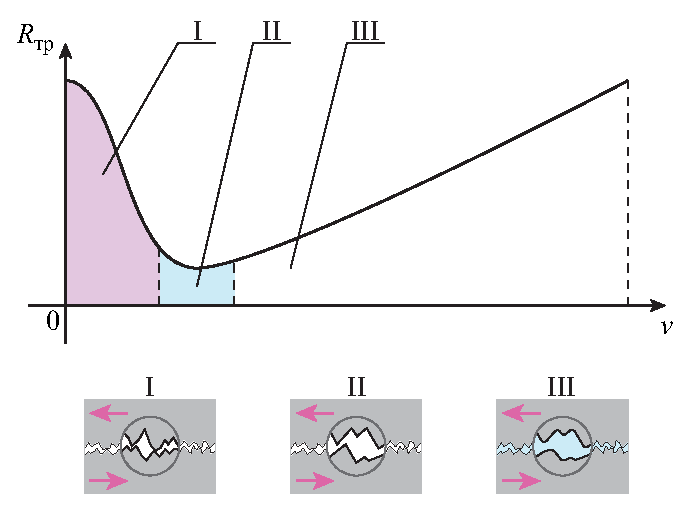
\includegraphics{part2/friction_model_demonstrate.eps}
    }
    \caption{Графическое представление модели трения}
    \label{fig:ch2/friction_model}
\end{figure}

Данная модель позволяет учесть ключевые особенности фрикционного взаимодействия в пневмоприводе:

Рассмотрим каждый компонент модели более подробно:
\begin{enumerate}
    \item Кулоновское трение:
          $$R_\text{к} = \mu_\text{к} N \text{sign}(v)$$
          где $\mu_\text{к}$ - коэффициент кулоновского трения, $N$ - нормальная сила. Кулоновское трение обеспечивает
          постоянную составляющую силы трения при установившемся движении;

    \item Статическое трение:
          $$R_\text{с} = \mu_\text{с} N \text{sign}(R_\text{вн})$$
          где $\mu_\text{с}$ - коэффициент статического трения, $R_\text{вн}$ - внешняя приложенная сила.
          Статическое трение препятствует началу движения при малых управляющих воздействиях;

    \item Эффект Штрибека:
          $$R_\text{ш} = (R_\text{с} - R_\text{к})e^{-\left|\frac{v}{v_\text{ш}}\right|^\delta}$$
          Эффект Штрибека описывает падение силы трения при переходе от состояния покоя к движению;

    \item Вязкое трение:
          $$R_\text{в} = \sigma_2 v$$
          где $\sigma_2$ - коэффициент вязкого трения. Вязкое трение зависит от скорости движения и преобладает при высоких скоростях.

\end{enumerate}

% Для определения параметров статической модели трения применяется следующий подход:

% \begin{enumerate}
%     \item Идентификация $R_\text{к}$ и $R_\text{в}$:
%           Проводятся тесты с постоянной скоростью движения. При установившемся движении сила трения описывается уравнением:
%           $$R_\text{тр} = R_\text{к} \text{sign}(v) + R_\text{в} v$$
%           Линейная регрессия по экспериментальным данным позволяет определить $R_\text{к}$ и $R_\text{в}$;

%     \item Идентификация $R_\text{с}$:
%           $R_\text{с}$ оценивается по максимальному значению силы трения при начале движения:
%           $$R_\text{с} = \max(|R_\text{тр}|) \text{ при } v \approx 0;$$

%     \item Идентификация $v_\text{ш}$ и $\delta$:
%           Параметры $v_\text{ш}$ и $\delta$ определяются путем минимизации среднеквадратичной ошибки между экспериментальной кривой зависимости силы трения от скорости и теоретической кривой:
%           $$\min_{v_\text{ш}, \delta} \sum_{i=1}^N (R_{\text{тр},i}^{\text{эксп}} - R_{\text{тр},i}^{\text{модель}}(v_\text{ш}, \delta))^2$$.
% \end{enumerate}

% Верификация статической модели трения осуществляется путем сравнения результатов моделирования
% с экспериментальными данными, полученными на реальном пневмоприводе. Проводится серия экспериментов
% с различными режимами движения, включая:

% \begin{enumerate}
%     \item Движение с постоянной скоростью;
%     \item Разгон и торможение;
%     \item Реверсивное движение;
%     \item kДвижение с малыми перемещениями.
% \end{enumerate}

% Для каждого эксперимента вычисляется среднеквадратичная ошибка между предсказанными и измеренными значениями силы трения:
% \begin{equation*}
%     RMSE = \sqrt{\frac{1}{N}\sum_{i=1}^N (R_{\text{тр},i}^{\text{эксп}} - R_{\text{тр},i}^{\text{модель}})^2}
% \end{equation*}

% Адекватность модели оценивается по совокупности критериев, включая RMSE, коэффициент
% детерминации $R^2$, и визуальный анализ графиков зависимости силы трения от скорости.
Данная статическая модель трения позволяет учесть основные нелинейные
эффекты фрикционного взаимодействия в пневмоприводе, что критически важно для
точного моделирования и эффективного управления системой. Однако следует отметить, что
статическая модель имеет ограничения в описании некоторых динамических эффектов, таких
как предварительное смещение и гистерезис, которые могут быть
существенными при прецизионном позиционировании.


\section{Моделирование силы реакции опоры}\label{sec:ch2/sec2/subsec5}

В контексте математического моделирования электропневматического привода существенную роль играет
адекватное описание силы реакции опоры. Данная сила возникает при контакте поршня пневмоцилиндра
с ограничителями хода и оказывает значительное влияние на динамику системы, особенно в крайних положениях.

Сила реакции опоры $R_\text{оп}$ может быть представлена как функция положения поршня $x$ и его скорости $\dot{x}$:
\begin{equation*}
    R_\text{оп} = f(x, \dot{x}).
\end{equation*}

При этом необходимо учитывать, что данная сила проявляется только при достижении
поршнем крайних положений. Таким образом, модель силы реакции опоры должна включать
условия её активации.

Наиболее распространенным подходом к моделированию силы реакции опоры является использование кусочно-линейной модели с учетом жесткости и демпфирования. Данная модель может быть описана следующим образом:
\begin{equation}\label{eq:ch2/support_reaction}
    R_\text{оп} = \begin{cases}
        k_\text{оп}(x - x_\text{мин}) + b_\text{оп}\dot{x},  & \text{если } x < x_\text{мин}                       \\
        0,                                                   & \text{если } x_\text{мин} \leq x \leq x_\text{макс} \\
        k_\text{оп}(x - x_\text{макс}) + b_\text{оп}\dot{x}, & \text{если } x > x_\text{макс}
    \end{cases}
\end{equation}

\section{Моделирование дискретных распределителей}\label{sec:ch2/sec3}

\subsection{Уравнения массового расхода рабочего тела}\label{sec:ch2/sec3/subsec1}
Массовый расход воздуха через дискретный распределитель
является ключевым параметром, определяющим динамику пневматической
системы. Для его описания используется модель, основанная на уравнении Сен-Венана-Ванцеля:
\begin{equation}
    G = \psi(p_1, p_2) \cdot u C_d F_e \frac{p_1}{\sqrt{RT_\text{вх}}},
\end{equation}
где
$G$ -- массовый расход воздуха;
$\psi(p_1, p_2)$ -- расходная функция;
$u$ -- положение золотника $(0 \div 1)$;
$C_d$ -- коэффициент расхода;
$F_e$ -- эффективная площадь проходного сечения;
$p_1$ -- давление на входе;
$p_2$ -- давление на выходе;
$R$ -- газовая постоянная для воздуха;
$T_\text{вх}$ -- температура воздуха на входе.

Ключевым элементом в данном уравнении является расходная функция $\psi(p_1, p_2)$, которая
учитывает влияние отношения давлений на входе и выходе распределителя
на массовый расход. Эта функция определяется следующим образом:
\begin{equation*}
    \psi(p_1, p_2) = \begin{cases}
        \sqrt{\frac{2\gamma}{\gamma-1}\left[\left(\frac{p_2}{p_1}\right)^{\frac{2}{\gamma}} - \left(\frac{p_2}{p_1}\right)^{\frac{\gamma+1}{\gamma}}\right]}, & \text{если } \frac{p_2}{p_1} > b_{кр}    \\
        \sqrt{\gamma \left(\frac{2}{\gamma+1}\right)^{\frac{\gamma+1}{\gamma-1}}},                                                                            & \text{если } \frac{p_2}{p_1} \leq b_{кр}
    \end{cases}
\end{equation*}
где
$\gamma$ -- показатель адиабаты для воздуха;
$b_{кр} = \left(\frac{2}{\gamma+1}\right)^{\frac{\gamma}{\gamma-1}}$ -- критическое отношение давлений.

Для наглядного представления характера изменения расходной функции
$\psi(p_1, p_2)$ в зависимости от отношения давлений $p_2/p_1$
приведен график представленны на рисунке \ref{fig:ch2/mass_flow_function}.
\begin{figure}
    \centerfloat{
        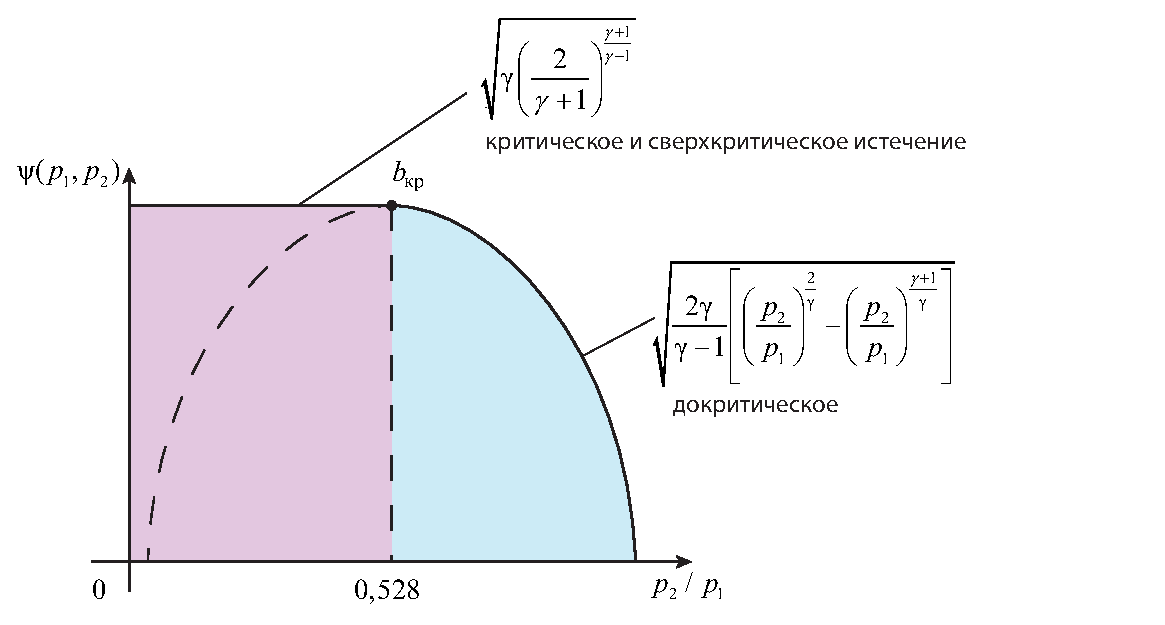
\includegraphics{part2/critical_gas_flow_chart.eps}
    }
    \caption{График расходной функции $\psi(p_1, p_2)$}
    \label{fig:ch2/mass_flow_function}
\end{figure}

На графике отчетливо видны две области: докритическое и закритическое течение, разделенные точкой
критического отношения давлений $b_{кр}$.

В области докритического течения ($p_2/p_1 > b_{кр}$) расход зависит от отношения давлений и
описывается нелинейной функцией. Здесь наблюдается плавное увеличение расхода с уменьшением отношения давлений.

В закритической области ($p_2/p_1 \leq b_{кр}$) расход достигает максимального
значения и остается постоянным независимо от дальнейшего снижения отношения давлений.
Это явление связано с достижением скорости потока воздуха
в самом узком сечении распределителя скорости звука.

Критическая точка $b_{кр}$ соответствует условию, при котором скорость потока
воздуха в самом узком сечении распределителя достигает скорости звука. Для
воздуха при нормальных условиях значение $b_{кр}$ составляет приблизительно \num{0.528}.
Эффективная площадь проходного сечения $F_\text{др}$ зависит от
положения запорно-регулирующего элемента распределителя и может
быть представлена как функция управляющего сигнала $u$:
\begin{equation*}
    F_\text{др} = F_{max} \cdot f(u),
\end{equation*}
где $F_{max}$ -- максимальная эффективная площадь проходного сечения;
$f(u)$ -- функция, описывающая зависимость площади от управляющего сигнала.

Представленная модель массового расхода позволяет точно описать процесс истечения
воздуха через дискретный распределитель в различных режимах работы
пневмопривода. Учет нелинейного характера расходной функции и
влияния критического отношения давлений особенно важен при анализе динамики
системы и разработке алгоритмов управления, обеспечивающих высокую точность
и быстродействие электропневматического привода.

\subsection{Динамика переключения распределителей}\label{sec:ch2/sec3/subsec2}

Процесс переключения дискретного распределителя характеризуется
определенной динамикой, которую необходимо учитывать для точного моделирования поведения
системы. Динамика переключения может быть описана дифференциальным уравнением первого порядка:
\begin{equation}\label{eq:ch2/switching_dynamics}
    \tau \frac{du}{dt} + u = u_{зад},
\end{equation}
где:
$u$ -- текущее положение запорно-регулирующего элемента;
$u_{зад}$ -- заданное положение (0 или 1 для дискретного распределителя);
$\tau$ -- постоянная времени переключения.

Альтернативно, для более точного описания динамики переключения
может быть использована модель второго порядка:
\begin{equation}
    \frac{d^2u}{dt^2} + 2\zeta\omega_n\frac{du}{dt} + \omega_n^2u = \omega_n^2u_{зад}
\end{equation}
где $\zeta$ -- коэффициент демпфирования;
$\omega_n$ -- собственная частота колебаний.

Учет динамики переключения позволяет моделировать такие эффекты, как задержка
срабатывания и дребезг контактов, которые могут оказывать
существенное влияние на поведение системы,
особенно при высокочастотном управлении.

Интеграция моделей массового расхода и динамики переключения
в общую математическую модель электропневматического привода
осуществляется путем их включения в уравнения
изменения давлений в полостях пневмоцилиндра \ref{eq:ch2/eq_pressure_system}.

В данной работе использована модель первого порядка для описания динамики переключения
поскольку она обеспечивает достаточно точное описание процесса переключения
и имеет простую структуру.


\section{Адаптация математической модели к эффективному численному расчету на ЭВМ}\label{sec:ch2/sec5}

Эффективное численное моделирование динамики электропневматического привода требует
оптимизации математической модели для выполнения расчетов на ЭВМ.
Данный этап критически важен для обеспечения высокой производительности
вычислений при проведении многочисленных итераций в задачах оптимизации,
анализа чувствительности и робастности системы управления.

Основные цели оптимизации математической модели включают:

\begin{enumerate}
    \item Снижение вычислительной сложности уравнений;
    \item Уменьшение времени выполнения расчетов;
    \item Повышение численной устойчивости алгоритмов;
    \item Эффективное использование параллельных вычислительных архитектур.
\end{enumerate}

Для достижения этих целей будут применены следующие методы:

\begin{enumerate}
    \item Векторизация уравнений;
    \item Упрощение и линеаризация нелинейных выражений;
    \item Предварительное вычисление констант и коэффициентов;
\end{enumerate}

\subsection{Векторизация уравнений}\label{sec:ch2/sec5/subsec1}
Векторизация уравнений представляет собой эффективный метод оптимизации вычислений,
позволяющий использовать преимущества SIMD-инструкций (Single Instruction, Multiple Data)
современных процессоров. Данный подход особенно актуален для математической
модели электропневматического привода с дискретными распределителями, где многие операции могут быть выполнены
параллельно \cite*{eichenberger2004simd} над несколькими элементами данных.

Основная идея векторизации заключается в преобразовании скалярных операций в
векторные, что позволяет обрабатывать несколько элементов данных
одновременно \cite*{nuzman2011vaporsimd}. В контексте рассматриваемой модели это означает переход от
поэлементных вычислений к операциям над векторами и матрицами.
Процесс векторизации начинается с представления состояния системы
в виде единого вектора. Для электропневматического привода
вектор состояния может быть записан как:

\begin{equation}
    \mathbf{y} = [x, v, p_1, p_2, T_1, T_2, x_{v1}, x_{v2}, x_{v3}, x_{v4}]^T.
\end{equation}

Система дифференциальных уравнений, описывающая динамику привода, преобразуется к векторной форме:
\begin{equation*}
    \frac{d\mathbf{y}}{dt} = \mathbf{f}(\mathbf{y}, t),
\end{equation*}
где $\mathbf{f}$ -- векторная функция, компоненты которой соответствуют правым частям исходных дифференциальных уравнений.

Векторизация уравнений массового расхода через распределители является одним из ключевых
элементов оптимизации. Вместо последовательного расчета расхода для
каждого распределителя, формируется вектор массовых расходов:

\begin{equation*}
    \mathbf{G} = \boldsymbol{\psi}(\mathbf{p}_1, \mathbf{p}_2) \odot \mathbf{u} \odot \mathbf{C}_d \odot \mathbf{F}_\text{др} \odot \frac{\mathbf{p}_{\text{вх}}}{\sqrt{R\mathbf{T}_{\text{вх}}}},
\end{equation*}
где $\odot$ -- поэлементное умножение векторов;
$\boldsymbol{\psi}(\mathbf{p}_1, \mathbf{p}_2)$ -- вектор-функция расходных характеристик;
$\mathbf{u}$ -- вектор управляющих сигналов;
$\mathbf{C}_d$ - вектор коэффициентов расхода;
$\mathbf{F}_\text{др}$ -- вектор эффективных площадей проходных сечений;
$\mathbf{p}_{вх}$ и $\mathbf{T}_{вх}$ -- векторы давлений и температур на входе распределителей соответственно.

Уравнения изменения давления в полостях цилиндра также подвергаются векторизации:

\begin{equation*}
    \frac{d\mathbf{p}}{dt} = \frac{\gamma R}{L} \odot \frac{\mathbf{T}}{\mathbf{V}} \odot
    \left(\mathbf{G}_{\text{вх}} - \mathbf{G}_{\text{вых}} - \frac{\mathbf{p}}{R\mathbf{T}} \odot \frac{d\mathbf{V}}{dt}\right),
\end{equation*}
где $\mathbf{p} = [p_1, p_2]^T$, $\mathbf{T} = [T_1, T_2]^T$, $\mathbf{V} = [V_1/L, V_2/L]^T$ --
векторы давлений, температур и нормализованных объемов полостей соответственно.

Векторизация затрагивает и уравнения изменения температуры в полостях:
\begin{equation*}
    \frac{d\mathbf{T}}{dt} = \frac{\mathbf{T}}{\mathbf{p}} \odot \frac{d\mathbf{p}}{dt} -
    (\gamma - 1) \frac{\mathbf{T}}{\bar{\mathbf{V}}} \odot \frac{d\bar{\mathbf{V}}}{dt}
\end{equation*}

Векторизация расчета расходной функции $\psi(p_1, p_2)$ осуществляется путем применения
векторных операций к отношениям давлений:
\begin{equation*}
    \boldsymbol{\psi}(\mathbf{p}_1, \mathbf{p}_2) = \begin{cases}
        \sqrt{\frac{2\gamma}{\gamma-1}\left[\left(\frac{\mathbf{p}_2}{\mathbf{p}_1}\right)^{\frac{2}{\gamma}} - \left(\frac{\mathbf{p}_2}{\mathbf{p}_1}\right)^{\frac{\gamma+1}{\gamma}}\right]}, & \text{если } \frac{\mathbf{p}2}{\mathbf{p}1} > b{кр},     \\
        \psi{макс},                                                                                                                                                                               & \text{если } \frac{\mathbf{p}_2}{\mathbf{p}1} \leq b{кр},
    \end{cases}
\end{equation*}
где операции возведения в степень и сравнения выполняются поэлементно.

Уравнения димаки золотника распределителей тоже можно векторизовать:
\begin{equation}
    \tau \frac{d\mathbf{u}}{dt} + \mathbf{u} = \mathbf{u}_\text{зад},
\end{equation}
где $\mathbf{u}$ -- вектор управляющих сигналов золотников;
$\mathbf{u}_\text{зад}$ -- вектор заданных значений управляющих сигналов.

Применение векторизации позволяет эффективно использовать SIMD-инструкции процессора,
что приводит к значительному ускорению вычислений. В зависимости от архитектуры процессора и
специфики реализации, ускорение может достигать 2-4 раза \cite*{tian2013simd} по сравнению с исходной скалярной версией.

\subsection{Оптимизация нелинейных функций}\label{sec:ch2/sec5/subsec2}

Так же важным этапом оптимизации является упрощение и линеаризация нелинейных функций,
которые могут оказывать существенное влияние на вычислительную сложность модели и деаль ее
жесткой. В контексте электропневматического привода, к нелинейным функцям относятся экспоненциальная
функция в модели трения, функция sign, реакция упоров и условные операции.

Для оптимизации вычисления экспоненциальной функции в модели трения предлагается использовать аппроксимацию Паде.
Данный метод обеспечивает высокую точность аппроксимации при сравнительно низкой вычислительной
сложности. Аппроксимация Паде для экспоненциальной функции может быть представлена в виде:

\begin{equation*}
    e^x \approx \frac{1 + \frac{x}{2} + \frac{x^2}{10} + \frac{x^3}{120}}{1 - \frac{x}{2} + \frac{x^2}{10} - \frac{x^3}{120}}.
\end{equation*}

Данная аппроксимация обеспечивает высокую точность в диапазоне $x \in [-2,5; 2,5]$,
что достаточно для моделирования эффекта Штрибека в рассматриваемой системе.

Функция sign, используемая в модели трения, может быть аппроксимирована
гладкой функцией для улучшения численной стабильности:

\begin{equation*}
    \text{sign}(x) \approx \tanh(kx),
\end{equation*}

где $k$ -- параметр, определяющий крутизну перехода. Рекомендуется выбирать k в диапазоне
$100 \div 1000$ для баланса между точностью аппроксимации и численной стабильностью.

Реакция упоров, обычно моделируемая с использованием условных операций, может быть
оптимизирована применением непрерывной аппроксимации:

\begin{equation*}
    R_\text{оп} = k_\text{оп}(x - x_\text{мин})\cdot S(x - x_\text{мин}) + k_\text{оп}(x - x_\text{макс})\cdot S(x - x_\text{макс}),
\end{equation*}
где $S(x)$ -- сглаживающая функция, например:

\begin{equation*}
    S(x) = \frac{1}{1 + e^{-\alpha x}},
\end{equation*}
где $\alpha$ -- параметр, определяющий крутизну перехода.

Для оптимизации условных операций в модели предлагается
использовать непрерывные аппроксимации. Например, функция
максимума может быть аппроксимирована как:

\begin{equation*}
    \max(a, b) \approx \frac{a + b + \sqrt{(a - b)^2 + \varepsilon}}{2},
\end{equation*}
где $\varepsilon$ -- малое положительное число, обеспечивающее гладкость функции.

Применяя предложенные оптимизации, уравнения реакции упоров и силы трения могут быть представлены в виде:

\begin{equation}
    \begin{alignedat}{2}
        R_\text{тр} & = \left[R_\text{к} + (R_\text{с} - R_\text{к})\frac{1 + \frac{z}{2} + \frac{z^2}{10} + \frac{z^3}{120}}{1 - \frac{z}{2} + \frac{z^2}{10} - \frac{z^3}{120}}\right]\tanh(k\dot{x}) + R_\text{в}\dot{x}, \\
        R_\text{оп} & = k_\text{оп}(x - x_\text{мин})\cdot \frac{1}{1 + e^{-\alpha(x - x_\text{мин})}} + k_\text{оп}(x - x_\text{макс})\cdot \frac{1}{1 + e^{-\alpha(x - x_\text{макс})}},
    \end{alignedat}
\end{equation}

\subsection{Аналитическое вычисление якобиана для численного решения ОДУ}\label{sec:ch2/sec5/subsec3}
Так же в рамках оптимизации модели использовалось аналитическое вычисление якобиана для
решателей ОДУ, что позволяет уменьшить количество вычислений и повысить численную стабильность.

Якобиан системы определяется как матрица частных производных:

\begin{equation}\label{eq:ch2/jacobian}
    J = \frac{\partial \mathbf{f}}{\partial \mathbf{y}} =
    \begin{pmatrix}
        \frac{\partial f_1}{\partial y_1}    & \frac{\partial f_1}{\partial y_2}    & \cdots & \frac{\partial f_1}{\partial y_{10}}    \\
        \frac{\partial f_2}{\partial y_1}    & \frac{\partial f_2}{\partial y_2}    & \cdots & \frac{\partial f_2}{\partial y_{10}}    \\
        \vdots                               & \vdots                               & \ddots & \vdots                                  \\
        \frac{\partial f_{10}}{\partial y_1} & \frac{\partial f_{10}}{\partial y_2} & \cdots & \frac{\partial f_{10}}{\partial y_{10}}
    \end{pmatrix}
\end{equation}

где $\mathbf{f}$ -- вектор-функция правых частей системы дифференциальных уравнений.

Ключевые элементы якобиана включают:
\begin{enumerate}
    \item Частные производные уравнения движения поршня:
          \begin{equation*}
              \begin{alignedat}{2}
                  \frac{\partial \dot{x}}{\partial x}   & = 0, & \quad \frac{\partial \dot{x}}{\partial v}   & = 1,                     \\
                  \frac{\partial \dot{v}}{\partial x}   & = 0, & \quad \frac{\partial \dot{v}}{\partial v}   & =
                  \frac{1}{M}(\mathbf{p}^T\mathbf{F} - p_\text{атм}(\mathbf{1}^T\mathbf{F}) - R_\text{тр} - R_\text{оп} - R_\text{вн}), \\
                  \frac{\partial \dot{v}}{\partial p_1} & = 0, & \quad \frac{\partial \dot{v}}{\partial p_2} & = 0.
              \end{alignedat}
          \end{equation*}

    \item Частные производные уравнений изменения давления:
          \begin{equation*}
              \begin{alignedat}{2}
                  \frac{\partial \dot{p}_i}{\partial x}    & = -\gamma p_i A_i / V_i,                                                           \\
                  \frac{\partial \dot{p}_i}{\partial v}    & = -\gamma p_i A_i / V_i,                                                           \\
                  \frac{\partial \dot{p}_i}{\partial p_i}  & = \gamma \left(R T_i \frac{\partial \dot{m}_i}{\partial p_i} - A_i v\right) / V_i, \\
                  \frac{\partial \dot{p}_i}{\partial T_i}  & = \gamma R \dot{m}_i / V_i,                                                        \\
                  \frac{\partial \dot{p}i}{\partial x{vj}} & = \gamma R T_i \frac{\partial \dot{m}i}{\partial x{vj}} / V_i;
              \end{alignedat}
          \end{equation*}

    \item Частные производные уравнений изменения температуры:

          \begin{equation*}
              \frac{\partial \dot{T}_i}{\partial y_j} = \frac{T_i}{p_i}\frac{\partial \dot{p}_i}{\partial y_j}
              - (\gamma - 1)\frac{T_i}{V_i}\frac{\partial \dot{V}_i}{\partial y_j};
          \end{equation*}
    \item Частные производные уравнений динамики золотников:
          \begin{equation*}
              \frac{\partial \dot{x}_{vi}}{\partial x_{vi}} = -1/\tau;
          \end{equation*}
\end{enumerate}

Запишем полный якобиан \ref{eq:ch2/jacobian} системы:

\begin{equation*}
    J = \begin{bmatrix}
        J_{xx}  & J_{xv}  & J_{xp}  & J_{xT}  & J_{xxv}  \\
        J_{vx}  & J_{vv}  & J_{vp}  & J_{vT}  & J_{vxv}  \\
        J_{px}  & J_{pv}  & J_{pp}  & J_{pT}  & J_{pxv}  \\
        J_{Tx}  & J_{Tv}  & J_{Tp}  & J_{TT}  & J_{Txv}  \\
        J_{xvx} & J_{xvv} & J_{xvp} & J_{xvT} & J_{xvxv}
    \end{bmatrix},
\end{equation*}

в данной матрице якобина каждый блок представляет собой подматрицу частных производных.
Рассмотрим каждый блок подробнее:
\begin{enumerate}
    \item $J_{xx}$ -- матрица размером $2 \times 2$
          \begin{equation*}
              J_{xx} = \begin{bmatrix}
                  0                                         & 1 \\
                  \frac{\partial F_\text{тр}}{\partial x}/M & 0
              \end{bmatrix};
          \end{equation*}

    \item $J_{xv}$ -- матрица размером $2 \times 2$
          \begin{equation*}
              J_{xv} = \begin{bmatrix}
                  0 & 0                                                                                                     \\
                  0 & \left( \frac{\partial F_\text{тр}}{\partial v}/M  + \frac{\partial F_\text{оп}}{\partial v}/M \right)
              \end{bmatrix};
          \end{equation*}

    \item $J_{xp}$ -- матрица размером $2 \times 2$
          \begin{equation*}
              J_{xp} = \begin{bmatrix}
                  0     & 0      \\
                  F_1/M & -F_2/M
              \end{bmatrix}
          \end{equation*};

    \item $J_{xT}$ -- матрица $O_{2,2}$;

    \item $J_{xxv}$ -- матрица $O_{3,3}$;

    \item $J_{vx} = J_{xv}^T$;

    \item $J_{vv} = J_{xv}$;

    \item $J_{vp} = J_{xp}$;

    \item $J_{vT} = J_{xT}$;

    \item $J_{vxv} = J_{xxv}$

    \item $J_{px}$ -- матрица размером $2 \times 2$
          \begin{equation*}
              J_{px} = \begin{bmatrix}
                  -\gamma p_1 F_1 / V_1 & -\gamma p_1 F_1 / V_1 \\
                  \gamma p_2 F_2 / V_2  & \gamma p_2 F_2 / V_2
              \end{bmatrix};
          \end{equation*}

    \item $J_{pv} = J_{px}$;

    \item $J_{pp}$ -- матрица размером $2 \times 2$
          \begin{equation*}
              J_{pp} = \begin{bmatrix}
                  \gamma R T_1 \frac{\partial \dot{m}_1}{\partial p_1} - F_1 v / V_1 & 0                                                                  \\
                  \0                                                                 & \gamma R T_2 \frac{\partial \dot{m}_2}{\partial p_2} - F_2 v / V_2
              \end{bmatrix};
          \end{equation*}

    \item $J_{pT}$ -- матрица размером $2 \times 2$

          \begin{equation*}
              J_{pT} = \begin{bmatrix}
                  \gamma R \dot{m}_1 / V_1 & 0                        \\
                  0                        & \gamma R \dot{m}_2 / V_2
              \end{bmatrix};
          \end{equation*}

    \item $J_{pxv}$ -- матрица размером $4 \times 2$

          \begin{equation*}
              J_{pxv} = \begin{bmatrix}
                  \gamma R T_1 \frac{\partial \dot{m}_1}{\partial x_{v1}}/V_1 & -\gamma R T_1 \frac{\partial \dot{m}_1}{\partial x_{v2}}/V_1 & 0                                                           & 0                                                            \\
                  0                                                           & 0                                                            & \gamma R T_2 \frac{\partial \dot{m}_2}{\partial x_{v3}}/V_2 & -\gamma R T_2 \frac{\partial \dot{m}_2}{\partial x_{v4}}/V_2
              \end{bmatrix};
          \end{equation*}

    \item $J_{Tx}$ -- матрица размером $2 \times 2$
          \begin{equation*}
              J_{Tx} = \begin{bmatrix}
                  T_1 J_{px,11}/p_1 & T_1 J_{px,12}/p_1 \\
                  T_2 J_{px,21}/p_2 & T_2 J_{px,22}/p_2
              \end{bmatrix};
          \end{equation*}

    \item $J_{Tv} = J_{Tx}$;

    \item $J_{Tp}$ -- матрица размером $2 \times 2$
          \begin{equation*}
              J_{Tp} = \begin{bmatrix}
                  T_1 J_{pp,11}/p_1 & 0                 \\
                  0                 & T_2 J_{pp,22}/p_2
              \end{bmatrix};
          \end{equation*}

    \item $J_{TT}$ -- матрица размером $2 \times 2$
          \begin{equation*}
              J_{TT} = \begin{bmatrix}
                  J_{pp,11} T_1/p_1 & 0                 \\
                  0                 & J_{pp,22} T_2/p_2
              \end{bmatrix};
          \end{equation*}

    \item $J_{Txv}$ -- матрица размером $3 \times 2$
          \begin{equation*}
              J_{Txv} = \begin{bmatrix}
                  T_1 J_{pxv,11}/p_1 & T_1 J_{pxv,12}/p_1 & 0                  & 0                  \\
                  0                  & 0                  & T_2 J_{pxv,23}/p_2 & T_2 J_{pxv,24}/p_2
              \end{bmatrix};
          \end{equation*}

    \item $J_{xvx} = J_{xvv} = J{xvp} = J_{xvT}$ -- матрица $O_{2,4}$;

    \item $J_{xvxv}$ -- матрица размером $4 \times 4$
          \begin{equation*}
              J_{xvxv} = \begin{bmatrix}
                  -1/\tau & 0       & 0       & 0       \\
                  0       & -1/\tau & 0       & 0       \\
                  0       & 0       & -1/\tau & 0       \\
                  0       & 0       & 0       & -1/\tau
              \end{bmatrix};
          \end{equation*}
\end{enumerate}

Применение якобиана для в методах численных численного интегрирования, таких как
BDF (Backward Differentiation Formula) и Radau, позволяет уменьшить количество вычислений
и повысить численную стабильность. В частности, использование якобиана позволяет
уменьшить количество вычислений правых частей системы, что особенно важно для жестких систем.

\section{Реализация математической модели}\label{sec:ch2/sec6}

Сведем полученные выражения в единую систему:

\begin{equation}
    \begin{cases}
        \begin{alignedat}{2}
            \frac{dx}{dt}          & = v                                                                                                                                                                                                    \\
            \frac{dv}{dt}          & = \frac{1}{M}(\mathbf{p}^T\mathbf{F} - p_\text{атм}(\mathbf{1}^T\mathbf{F}) - R_\text{тр} - R_\text{оп} - R_\text{вн} )                                                                                \\                                                                                                                   \\
            \frac{d\mathbf{p}}{dt} & = \frac{\gamma R}{L} \odot \frac{\mathbf{T}}{\bar{\mathbf{V}}} \odot \left(\mathbf{G}_{\text{вх}} - \mathbf{G}_{\text{вых}} - \frac{\mathbf{p}}{R\mathbf{T}} \odot \frac{d\bar{\mathbf{V}}}{dt}\right) \\
            \frac{d\mathbf{T}}{dt} & = \frac{\mathbf{T}}{\mathbf{p}} \odot \frac{d\mathbf{p}}{dt} - (\gamma - 1) \frac{\mathbf{T}}{\bar{\mathbf{V}}} \odot \frac{d\bar{\mathbf{V}}}{dt}                                                     \\
            \mathbf{G}             & = \boldsymbol{\psi}(\mathbf{p}_1, \mathbf{p}_2) \odot \mathbf{u} \odot \mathbf{C}_d \odot \mathbf{F}_\text{др} \odot \frac{\mathbf{p}_{\text{вх}}}{\sqrt{R\mathbf{T}_\text{вх}}}                       \\
            R_\text{тр}            & = \left[R_\text{к} + (R_\text{с} - R_\text{к})\frac{1 + \frac{z}{2} + \frac{z^2}{10} + \frac{z^3}{120}}{1 - \frac{z}{2} + \frac{z^2}{10} - \frac{z^3}{120}}\right]\tanh(k\dot{x}) + R_\text{в}\dot{x}  \\
            R_\text{оп}            & = k_\text{оп}(x - x_\text{мин})\cdot \frac{1}{1 + e^{-\alpha(x - x_\text{мин})}} + k_\text{оп}(x - x_\text{макс})\cdot \frac{1}{1 + e^{-\alpha(x - x_\text{макс})}}                                    \\
            \mathbf{u}_\text{зад}  & = \tau \frac{d\mathbf{u}}{dt} + \mathbf{u}
        \end{alignedat}
    \end{cases}
\end{equation}
где
$\mathbf{p} = [p_1, p_2]^T$ -- вектор давлений в полостях цилиндра;
$\mathbf{F} = [F_1, -F_2]^T$ -- вектор эффективных площадей поршня;
$\mathbf{1} = [1, 1]^T$ -- единичный вектор;
$p_\text{атм}$ -- атмосферное давление (скалярная величина);
$(\mathbf{1}^T\mathbf{F}) = F_1 - F_2$ -- результат векторного произведения, дающий разность площадей;
$\mathbf{u}$ -- вектор управляющих сигналов золотников;
$\mathbf{u}_\text{зад}$ -- вектор заданных значений управляющих сигналов;

Реализация математической модели электропневматического привода осуществляется с использованием языка программирования Python
и специализированных библиотек для научных вычислений. Основой реализации служит класс \texttt{ElectroPneumaticActuator},
который инкапсулирует параметры системы и методы для моделирования ее динамики.

Структура класса включает конструктор для инициализации параметров привода, методы для расчета производных состояния системы,
а также вспомогательные функции для вычисления отдельных компонентов модели, таких как массовые расходы, силы трения и реакции упоров.
Ключевым элементом реализации является метод \texttt{calculate\_derivatives}, который формирует систему дифференциальных уравнений,
описывающих динамику привода.

\begin{ListingEnv}[!h]% настройки floating аналогичны окружению figure
    \captiondelim{ } % разделитель идентификатора с номером от наименования
    \caption{ \protect\python}\label{lst:hwbeauty}
    % окружение учитывает пробелы и табуляции и применяет их в сответсвии с настройками
    \begin{lstlisting}[language={Python}]
import numpy as np
from scipy.integrate import solve_ivp
from numba import njit

class ElectroPneumaticActuator:
    def __init__(self, params):
        self.m = params['m']  # Масса подвижных частей
        self.A1 = params['A1']  # Эффективная площадь поршня со стороны штока
        # Остальные параметры...

    @njit
    def calculate_derivatives(self, t, y, u):
        x, v, p1, p2, T1, T2 = y

        V1 = self.V0 + self.A1 * x
        V2 = self.V0 + self.A2 * (self.L - x)
        # Расчет отсальных состояний...
        return np.array([dx, dv, dp1, dp2, dT1, dT2])

    @njit
    def mass_flow(self, p_up, p_down, T_up, u):
        # Реализация расчета массового расхода...
    # Реализация остальных методов...

    def solve(self, t_span, y0, u_func):
        sol = solve_ivp(
            lambda t, y: self.calculate_derivatives(t, y, u_func(t)),
            t_span, y0, method='RK45', rtol=1e-6, atol=1e-9
        )
        return sol
    \end{lstlisting}
\end{ListingEnv}%

Центральным элементом модели, как было сказано выше, является метод \texttt{calculate\_derivatives},
который формирует систему дифференциальных уравнений, описывающих динамику привода.
Этот метод учитывает изменение объемов полостей цилиндра, массовые расходы через
распределители, силы, действующие на поршень, и термодинамические процессы в системе.

Метод \texttt{solve} обеспечивает интеграцию различных алгоритмов управления в процесс моделирования,
что позволяет проводить сравнительный анализ эффективности различных стратегий управления приводом.

Полная реализация модели, включая детальные расчеты массовых расходов, сил трения и
различных алгоритмов управления, представлена в приложении к диссертации \fixme{организовать приложение}.

Управление приводом, согласно вышенаписанному, осуществляется путем задания управляющего сигнала $\mathbf{u}$,
который представляет собой вектор состояний дискретных распределителей. Поскольку в рассматриваемой системе используется четыре распределителя, то $\mathbf{u} \in {0,1}^4$, где 0 соответствует
закрытому состоянию распределителя, а 1 -- открытому.

Для реализации различных алгоритмов управления в модель введен абстрактный базовый класс~\texttt{AbstractController},
от которого наследуются конкретные реализации контроллеров. Этот подход обеспечивает гибкость при исследовании
и сравнении различных стратегий управления. Структура класса AbstractController определена следующим образом:

\begin{ListingEnv}[!h]% настройки floating аналогичны окружению figure
    \captiondelim{ } % разделитель идентификатора с номером от наименования
    \caption{ \protect\python}\label{lst:AbstractControllerClass}
    \begin{lstlisting}[language={Python}]
from abc import ABC, abstractmethod

class AbstractController(ABC):
    @abstractmethod
    def calculate_control(self, t, y, y_ref):
        pass

    @abstractmethod
    def convert_to_valve_states(self, u):
        pass
    \end{lstlisting}
\end{ListingEnv}%

Метод \textttt{calculate\_control} вычисляет управляющее воздействие на основе текущего состояния системы \texttt{y},
заданного значения \texttt{y\_ref} и времени \texttt{t}.
Метод \texttt{conver\_to\_valve\_states} преобразует вычисленное управляющее воздействие
в конкретные состояния распределителей.

\section{Верификация математической модели}\label{sec:ch2/sec7}
Верификация математической модели  представляет собой неотъемлемый этап разработки, направленный на подтверждение адекватности
и точности полученного математического описания. Процесс верификации включает в себя комплекс методов и подходов,
позволяющих оценить соответствие модели реальному объекту в рамках принятых допущений и ограничений.

Основной целью верификации является подтверждение способности модели корректно отражать физические процессы,
происходящие в электропневматическом приводе, и обеспечивать достоверные результаты при решении задач анализа и синтеза систем управления.
В отсутствие экспериментальных данных, предварительная верификация базируется на теоретическом анализе,
численном моделировании.

Верификация данных происходила на основе следующих параметров модели, которые согласованны
с характерными параметрами экпериментального стенда и пердставлены в
таблице \ref{tab:ch2/extended_parameters}.

\begin{table}[h]
    \centering
    \caption{Расширенные параметры моделирования электропневматического привода}
    \small
    \begin{tabular}{lccl}
        \textbf{Параметр}                & \textbf{Обозначение}                      & \textbf{Значение}     & \textbf{Размерность} \\
        \midrule
        Масса подвижных частей           & $M$                                       & 6.0                   & кг                   \\
        Ход поршня                       & $L$                                       & 0.3                   & м                    \\
        Диаметр поршня                   & $D_\text{п}$                              & 0.032                 & м                    \\
        Диаметр штока                    & $d_\text{шт}$                             & 0.012                 & м                    \\
        Площадь поршня со стороны штока  & $F_2 = \pi(D_\text{п}^2-d_\text{шт}^2)/4$ & $7.07 \times 10^{-4}$ & м$^2$                \\
        Площадь поршня со стороны крышки & $F_1 = \pi D_\text{п}^2/4$                & $8.04 \times 10^{-4}$ & м$^2$                \\
        Давление питания                 & $p_\text{п}$                              & $6 \times 10^5$       & Па                   \\
        Атмосферное давление             & $p_\text{атм}$                            & $1 \times 10^5$       & Па                   \\
        Газовая постоянная воздуха       & $R$                                       & 287                   & Дж/(кг$\cdot$К)      \\
        Температура воздуха              & $T_\text{атм}$                            & 293                   & К                    \\
        Показатель адиабаты              & $\gamma$                                  & 1.4                   & -                    \\
        Коэффициент расхода              & $C_d$                                     & 0.7                   & -                    \\
        Эффективная площадь клапана      & $A_v$                                     & $1.2 \times 10^{-6}$  & м$^2$                \\
        \midrule
        \multicolumn{4}{l}{\textbf{Параметры силы трения:}}                                                                         \\
        \midrule
        Сила сухого трения               & $F_c$                                     & 50                    & Н                    \\
        Сила трения покоя                & $F_s$                                     & 60                    & Н                    \\
        Коэффициент вязкого трения       & $\sigma_2$                                & 100                   & Н$\cdot$с/м          \\
        Скорость Штрибека                & $v_s$                                     & 0.01                  & м/с                  \\
        Показатель степени Штрибека      & $\delta$                                  & 2                     & -                    \\
        \midrule
        \multicolumn{4}{l}{\textbf{Параметры реакции опор:}}                                                                        \\
        \midrule
        Коэффициент жесткости опоры      & $k_\text{оп}$                             & $1 \times 10^6$       & Н/м                  \\
        Коэффициент демпфирования опоры  & $b_\text{оп}$                             & 1000                  & Н$\cdot$с/м          \\
        Координата нижнего упора         & $x_\text{мин}$                            & 0                     & м                    \\
        Координата верхнего упора        & $x_\text{макс}$                           & 0.3                   & м                    \\
        \midrule
    \end{tabular}
    \label{tab:ch2/extended_parameters}
\end{table}

\subsection{Теоретические основы верификкаци}\label{sec:ch2/sec7/subsec1}
Процесс верификации основывается на следующих ключевых принципах:

\begin{enumerate}
    \item Принцип физической непротиворечивости, требующий соответствия модели фундаментальным законам механики и пневматики;
    \item Принцип математической корректности, предполагающий отсутствие ошибок в формулировке уравнений и их решении;
    \item Принцип консервативности, обеспечивающий выполнение законов сохранения массы и энергии в модели;
    \item Принцип устойчивости решения, гарантирующий сходимость численных методов при различных начальных условиях и параметрах системы.
\end{enumerate}

Методологический базис верификации включает:

\begin{enumerate}
    \item Аналитический анализ структуры модели и ее соответствия физическим законам;
    \item Численное моделирование с исследованием сходимости и устойчивости решения;
    \item Анализ предельных случаев и упрощенных режимов работы системы;
    \item Оценку чувствительности модели к вариациям параметров.
\end{enumerate}

Математически процесс верификации может быть формализован как задача минимизации функционала
ошибки между результатами моделирования и теоретическими предсказаниями для известных частных случаев:
\begin{equation*}
    J = \min_{\theta} \sum_{i=1}^{N} \left| f_{\text{модель}}(x_i, \theta) - f_{\text{теория}}(x_i) \right|^2,
\end{equation*}
где $f_{\text{модель}}$ -- функция, описывающая выход модели;
$f_{\text{теория}}$ -- теоретически предсказанное значение;
$x_i$ -- входные параметры;
$\theta$ -- параметры модели;
$N$ -- количество точек сравнения.

Выбор методов верификации обусловлен спецификой исследуемой системы и включает:

\begin{enumerate}
    \item Проверку размерностей и единиц измерения всех величин в уравнениях модели.
    \item    Анализ асимптотического поведения модели при предельных значениях параметров.
    \item Исследование сходимости численного решения при измельчении шага интегрирования.
    \item Оценку энергетического баланса системы и соблюдения закона сохранения массы.
\end{enumerate}

\subsection{Проверка маетматической корректности}\label{sec:ch2/sec7/subsec2}

Проверка математической корректности модели электропневматического привода с дискретными распределителями осуществляется посредством следующих процедур:

\begin{enumerate}
    \item Анализ размерностей и единиц измерения;
    \item Верификация согласованности уравнений с законами сохранения;
    \item Оценка физической непротиворечивости уравнений;
    \item Проверка граничных условий и начальных значений;
    \item Анализ непрерывности и дифференцируемости функций.
\end{enumerate}

Каждая процедура направлена на выявление потенциальных ошибок в математическом описании
системы и обеспечение соответствия модели фундаментальным физическим принципам.

Основыне этапы проверки математической корректности модели подробнее:

\paragraph{Анализ размерностей и единиц измерения.}

Проверка согласованности размерностей всех величин, входящих в уравнения модели, осуществляется с использованием метода анализа размерностей. Для каждого уравнения модели выполняется проверка:
\begin{equation*}
    [LHS] = [RHS],
\end{equation*}
где $[LHS]$ и $[RHS]$ -- размерности левой и правой частей уравнения соответственно.

\paragraph{Верификация согласованности уравнений с законами сохранения.}

Проверяется выполнение законов сохранения массы и энергии. Для закона сохранения массы в пневматической системе:
\begin{equation*}
    \frac{d}{dt}\int_V \rho dV + \oint_S \rho \mathbf{v} \cdot d\mathbf{S} = 0,
\end{equation*}
где $\rho$ -- плотность воздуха; $V$ -- объем системы; $\mathbf{v}$ -- скорость потока; $S$ -- поверхность контрольного объема.

Для закона сохранения энергии:
\begin{equation*}
    \frac{d}{dt}(E_k + E_p + U) = W_{\text{внеш}} - Q
\end{equation*}
где $E_k$ -- кинетическая энергия;
$E_p$ -- потенциальная энергия;
$U$ -- внутренняя энергия;
$W_{\text{внеш}}$ -- работа внешних сил;
$Q$ -- теплота, переданная системе.

\paragraph{Оценка физической непротиворечивости уравнений.}

В рамках оценки физической непротиворечивости уравнений проводится проверка
выполнения второго закона термодинамики для адиабатного процесса, в частности, принципа неубывания энтропии.

Для адиабатной системы изменение энтропии должно удовлетворять неравенству:
\begin{equation*}
    \Delta S \geq 0
\end{equation*}
где $\Delta S$ -- изменение энтропии системы.

Проверка неубывания энтропии осуществляется следующим образом:

\begin{enumerate}
    \item Вычисление изменения энтропии для каждой полости цилиндра на каждом шаге интегрирования:
          \begin{equation*}
              \Delta S_i = m_i c_v \ln\left(\frac{T_{i,k+1}}{T_{i,k}}\right) + m_i R \ln\left(\frac{V_{i,k+1}}{V_{i,k}}\right),
          \end{equation*}
          где $m_i$ -- масса газа в i-й полости;
          $c_v$ -- удельная теплоемкость при постоянном объеме;
          $T_{i,k}$ и $V_{i,k}$ -- температура и объем i-й полости на k-м шаге интегрирования.

    \item Расчет производства энтропии за счет необратимых процессов, включая трение и дросселирование газа:
          \begin{equation*}
              \Delta S_{\text{irr}} = \frac{F_{\text{тр}} \Delta x}{T_{\text{ср}}} + \sum_j G_j R \ln\left(\frac{p_{\text{вых},j}}{p_{\text{вх},j}}\right),
          \end{equation*}
          где $F_{\text{тр}}$ -- сила трения;
          $\Delta x$ -- перемещение;
          $T_{\text{ср}}$ -- средняя температура;
          $G_j$ -- массовый расход через j-й распределитель;
          $p_{\text{вх},j}$ и $p_{\text{вых},j}$ -- давления на входе и выходе j-го распределителя.

    \item Проверка условия неубывания суммарной энтропии системы:
          \begin{equation*}
              \Delta S_{\text{total}} = \sum_i \Delta S_i + \Delta S_{\text{irr}} \geq 0.
          \end{equation*}
\end{enumerate}

Дополнительно проверяется выполнение уравнения адиабатного процесса для каждой полости:
\begin{equation*}
    pV^{\gamma} = \text{const}.
\end{equation*}

\paragraph{Проверка граничных условий и начальных значений.}

Осуществляется верификация корректности заданных граничных условий и начальных значений.
Для пневматической системы это включает проверку согласованности давлений на границах системы:
\begin{equation*}
    p_{\text{вх}} \geq p_i \geq p_{\text{вых}},
\end{equation*}
где $p_{\text{вх}}$ -- давление источника;
$p_i$ - давление в i-й полости;
$p_{\text{вых}}$ -- давление на выходе (обычно атмосферное).

\paragraph{Анализ непрерывности и дифференцируемости функций.}

Проверяется непрерывность и дифференцируемость всех функций, входящих в модель, особенно в точках переключения
режимов работы распределителей. Для функции расхода через распределитель $G(p_1, p_2)$ должно выполняться условие:
\begin{equation*}
    \lim_{p_2 \to p_1^-} G(p_1, p_2) = \lim_{p_2 \to p_1^+} G(p_1, p_2)
\end{equation*}

\subsection{Анализ предельных случаев}\label{sec:ch2/sec7/subsec3}

Анализ предлельных случаев позволяет оценить корректность поведения модели в экстремальных условиях
и проверить соответствие результатов теоретическим предсказаниям.

В рамках исследования предельных случаев рассматриваются следующие аспекты:

\paragraph{Поведение системы при экстремальных значениях параметров.}

Проводится серия численных экспериментов с использованием разработанной математической модели
при предельных значениях ключевых параметров системы. К таким параметрам относятся:
\begin{itemize}
    \item Давление питания $p_s$:
          При $p_s \rightarrow 0$ ожидается отсутствие движения поршня.
          При $p_s \rightarrow \infty$ следует наблюдать ограничение скорости движения поршня, обусловленное силами трения и инерцией.
    \item Масса подвижных частей $m$:
          При $M \rightarrow 0$ динамика системы должна определяться преимущественно силами трения.
          При $M \rightarrow \infty$ ожидается значительное замедление движения поршня.
    \item Коэффициенты трения:
          При стремлении коэффициентов трения к нулю система должна демонстрировать колебательное поведение с минимальным затуханием.
          При значительном увеличении коэффициентов трения ожидается апериодический характер движения с возможным возникновением эффекта "прилипания-скольжения".
    \item Эффективные площади проходных сечений распределителей:
          При $F_\text{др} \rightarrow 0$ должно наблюдаться существенное замедление динамики системы.
          При $F_\text{др} \rightarrow \infty$ ожидается приближение характеристик системы к случаю с идеальным источником давления.
\end{itemize}

\subsection{Оценка физичности результатов моделирования}\label{sec:ch2/sec7/subsec4}

\paragraph{Проверка размерностей и единиц измерения.}
Рассматриваются размерности основных физических величин, используемых в модели:

\begin{itemize}
    \item Длина: $ [L] = \text{м}$;
    \item Время: $ [T] = \text{с}$;
    \item Масса: $ [M] = \text{кг}$;
    \item Сила: $ [F] = \text{кг}\cdot\text{м}/\text{с}^2$;
    \item Давление: $ [P] = \text{кг}/(\text{м}\cdot\text{с}^2)$;
    \item Температура: $ [\Theta] = \text{К}$.
\end{itemize}}

Анализ размерностей для каждого уравнения системы:
\begin{itemize}
    \item Уравнение движения поршня: $ [M\cdot L/T^2] = [P\cdot L^2] + [F]$;
    \item Уравнение изменения давления: $ [P/T] = [M/(L^2\cdot T^2)] $;
    \item Уравнение изменения температуры: $ [\Theta/T] = [\Theta/T]$;
    \item Уравнение массового расхода: $  [M/T] = [L^2] \cdot [P] / [L/T] = [M/T] $;
    \item Уравнение силы трения: $  [F] = [F] + [F\cdot T/L] \cdot [L/T] = [F] $;
    \item Уравнение реакции опоры: $  [F] = [F/L] \cdot [L] = [F] $;
    \item Уравнение динамики золотников: $  [1] = [1]$.
\end{itemize}

Проведенный анализ подтверждает согласованность размерностей во всех уравнениях математической модели.
Это свидетельствует о корректности формулировки модели с точки зрения физических единиц измерения.

\subsection{Заключение о достоверности модели}\label{sec:ch2/sec7/subsec5}
           % Глава 2
\chapter{МЕТОДЫ УПРАВЛЕНИЯ ЭЛЕКТРОПНЕВМАТИЧЕСКИМ ПРИВОДОМ С ДИСКРЕТНЫМ УПРАВЛЕНИЕМ}\label{ch:ch3}
Управление электропневматическими приводами с дискретными распределителями представляет
собой комплексную задачу, обусловленную нелинейной динамикой пневматических систем и
дискретным характером управляющих воздействий. Эффективное решение данной задачи требует
применения специализированных алгоритмов, способных обеспечить высокую точность позиционирования и
быстродействие системы при ограниченном наборе управляющих состояний. Особый интерес представляет адаптация
классических методов управления к специфике дискретных пневматических систем.

В рамках настоящего исследования рассматривается широкий спектр подходов к управлению электропневматическими
приводами, включающий как современные адаптивные методы, так и модифицированные
классические алгоритмы. Исследуются скользящее управление, прогнозное управление,
нечеткое управление, нейросетевое управление, а также применение широтно-импульсной модуляции (ШИМ)
в сочетании с классическими регуляторами, такими как ПИД-регулятор и его модификации.
Выбор данных методов обусловлен необходимостью комплексного анализа возможностей оптимизации управления
с учетом специфики дискретных пневматических систем. Каждый из рассматриваемых подходов обладает
уникальными преимуществами и ограничениями, детальное изучение которых позволит сформировать
всестороннее представление о перспективах совершенствования алгоритмов управления
электропневматическими приводами с дискретными распределителями.

\section{ШИМ управление с использование ПИД регулятора}\label{sec:ch3/sec1}

\subsection{Принципы реализации ШИМ в пневматических системах с дискретным управлением}\label{subsec:ch3/sec1/sub1}
Широтно-импульсная модуляция (ШИМ) представляет собой метод формирования квазинепрерывного
управляющего воздействия в системах с дискретными исполнительными элементами.
В контексте пневматических систем с дискретными распределителями применение ШИМ
позволяет преодолеть ограничения, связанные с бинарным характером управления, и обеспечить более
точное регулирование положения и скорости исполнительного механизма.

Механизм формирования квазинепрерывного управляющего воздействия
посредством ШИМ основан на периодическом переключении дискретных
распределителей с определенной частотой и скважностью.

Математически это может быть описано следующим образом:

\begin{equation*}
    u(t) = \begin{cases}
        1, & 0 \leq t < \alpha T \\
        0, & \alpha T \leq t < T
    \end{cases}
\end{equation*}
где $u(t)$ -- управляющий сигнал;
$T$ -- период ШИМ;
$\alpha$ -- коэффициент заполнения $0 \leq \alpha \leq 1$.

На рисунке \ref{fig:ch3:pwm_example} показаны временные диаграммы ШИМ-сигнала
с различными значениями коэффициента заполнения.

\begin{figure}[ht]
    \centerfloat{
        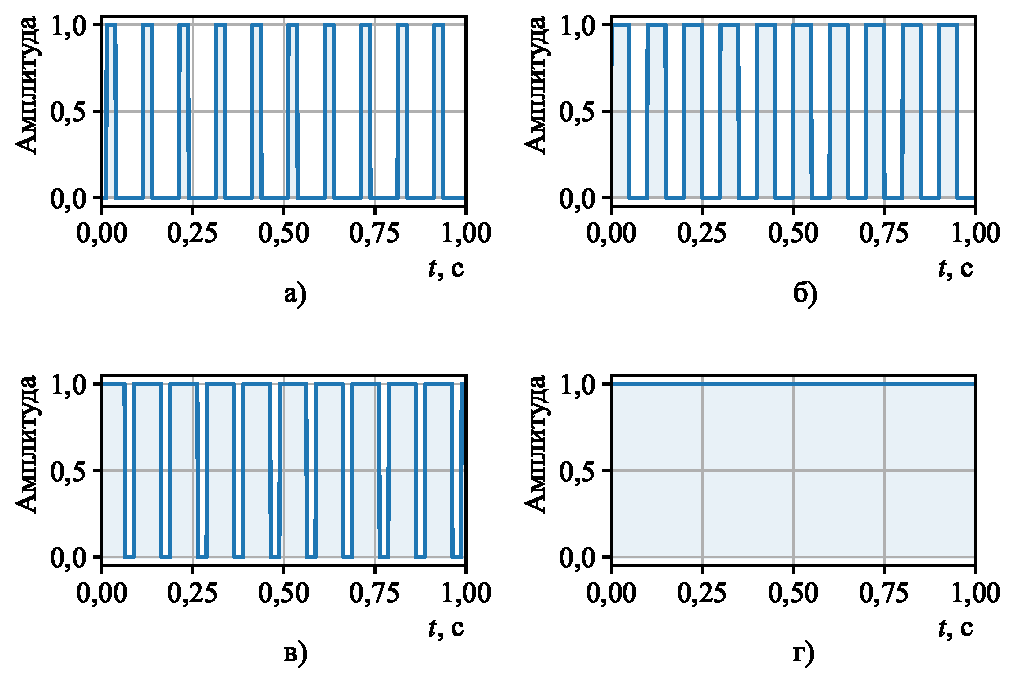
\includegraphics[]{part3/pwm_signal_skewness.pdf}
    }
    \caption{Примеры ШИМ-сигнала с различными значениями коэффициента заполнения}
    \label{fig:ch3:pwm_example}
\end{figure}

Среднее значение управляющего воздействия за период определяется как:
\begin{equation*}
    \bar{u} = \frac{1}{T} \int_0^T u(t) dt = \alpha,
\end{equation*}

Влияние частоты ШИМ на динамику пневмопривода является критическим фактором при
проектировании системы управления. С увеличением частоты ШИМ улучшается
гладкость управляющего воздействия, что способствует снижению пульсаций давления
и повышению точности позиционирования. Однако чрезмерно высокая частота может привести
к повышенному износу распределителей и увеличению энергопотребления.

На рисунке \ref{fig:ch3:pwm_pressure_response} представлены графики изменения
давления в пневмоцилиндре при различных частотах ШИМ.

\begin{figure}[ht]
    \centerfloat{
        % \includegraphics[]{part3/pwm_pressure_response.pdf}
    }
    \caption{Влияние частоты ШИМ на пульсации давления в пневмоцилиндре}
    \label{fig:ch3:pwm_pressure_response}
\end{figure}

Для анализа влияния частоты ШИМ на динамику системы может быть использована передаточная функция эквивалентного непрерывного звена:
\begin{equation*}
    W_{\text{ШИМ}}(s) = \frac{1 - e^{-sT}}{sT},
\end{equation*}
где $s$ -- комплексная переменная преобразования Лапласа.
Особенности применения ШИМ для различных типов дискретных
распределителей обусловлены их конструктивными характеристиками и
динамическими свойствами. На рисунке \ref{fig:ch3:pwm_valve_response} показаны
характеристики переходных процессов для распределителей с различным быстродействием.

\begin{figure}[ht]
    \centerfloat{
        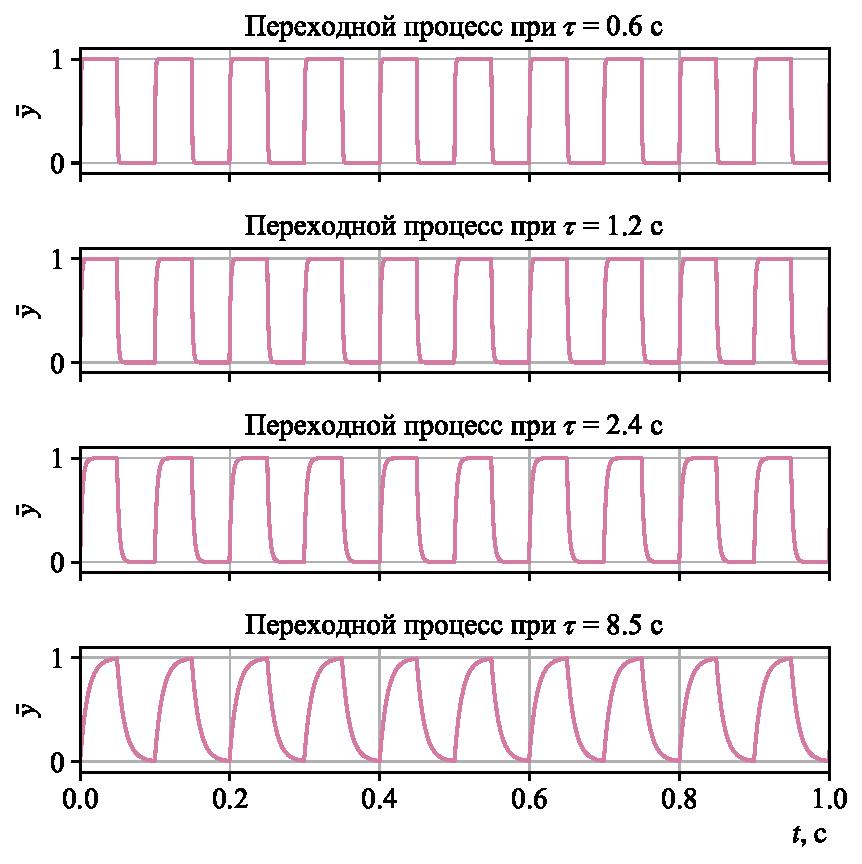
\includegraphics[]{part3/pwm_valve_response.pdf}
    }
    \caption{Характеристики переходных процессов для различных типов дискретных распределителей}
    \label{fig:ch3:pwm_valve_response}
\end{figure}

При выборе параметров ШИМ необходимо учитывать соотношение между
периодом ШИМ и динамическими характеристиками распределителя:
\begin{equation*}
T_{ШИМ} \geq k\tau_{\text{р}},
\end{equation*}
где $\tau_{\text{р}}$ -- время реакции распределителя;
$k$ -- коэффициент запаса (обычно $k \geq 2$).

\subsection{Реализация ПИД-регулирования для пневмоприводов с дискретными распределителями}\label{subsec:ch3/sec1/sub2}
Применение ШИМ в пневмоприводах с дискретными распределителями открывает
возможность использования алгоритмов управления,
изначально разработанных для непрерывных систем.
Одним из наиболее эффективных и широко применяемых методов является
пропорционально-интегрально-дифференциальное (ПИД) регулирование.

Структура ПИД-регулятора для пневмопривода
с дискретными распределителями может быть представлена следующей схемой:
\begin{figure}[ht]
   \centerfloat{
    %    \includegraphics[]{part3/pid_pwn_control.pdf}
    \caption{Структурная схема ПИД-регулятора с ШИМ управлением}
    \label{fig:ch3:pid_pwm_control}
\end{figure}
В данной схеме выходной сигнал ПИД-регулятора преобразуется в коэффициент
заполнения ШИМ, который управляет дискретными распределителями
пневмопривода. Этот подход позволяет достичь высокой точности
управления, характерной для непрерывных систем, в условиях
дискретного исполнительного механизма.

Математическая модель ПИД-регулятора в дискретной форме описывается уравнением:
\begin{equation*}
u[k] = K_p e[k] + K_i T_s \sum_{i=0}^k e[i] + K_d \frac{e[k] - e[k-1]}{T_s},
\end{equation*}
где
$u[k]$ -- управляющий сигнал на k-ом шаге;
$e[k]$ -- ошибка регулирования на k-ом шаге;
$K_p$, $K_i$, $K_d$ -- коэффициенты пропорциональной, интегральной и
дифференциальной составляющих соответственно;
$T_s$ -- период дискретизации.

Выходной сигнал ПИД-регулятора преобразуется в коэффициент заполнения ШИМ согласно формуле:
\begin{equation*}
\alpha = \frac{u[k] + u_{max}}{2u_{max}},
\end{equation*}
где $u_{max}$ -- максимальное значение управляющего сигнала.

\subsection{Модифицированные структуры ПИД регулятора}\label{subsec:ch3/sec1/sub3}
\subsection{Применение усреднителя Смита для компенсации запаздывания}\label{subsec:ch3/sec1/sub4}
\subsection{Каскадные и комбинированные структуры ПИД регуляторов}\label{subsec:ch3/sec1/sub5}
\subsection{Математическое описание и анализ динамических характеристик}\label{subsec:ch3/sec1/sub6}

\section{Управление в скользящих режимах}\label{sec:ch3/sec2}

\section{Нечеткое управление}\label{sec:ch3/sec3}

\section{Прогнозное управление}\label{sec:ch3/sec4}
           % Глава 3
\chapter{МЕТОДОЛОГИЯ МНОГОКРИТЕРИАЛЬНОЙ ОПТИМИЗАЦИИ ПАРАМЕТРОВ ПНЕВМОПРИВОДА}\label{ch:ch4}

Задача многокритериальной оптимизации параметров пневмопривода
заключается в нахождении оптимального набора параметров системы
управления, обеспечивающего баланс между несколькими конфликтующими
критериями качества работы привода. Основными критериями в данном случае
выступают точность позиционирования выходного звена пневмопривода и
частота переключений дискретных пневмораспределителей, которые определяют
долговечность и энергопотребление системы. Оптимизация параметров управления
направлена на минимизацию ошибок позиционирования при минимально возможном числе
переключений, что позволяет продлить срок службы оборудования и снизить износ компонентов.

\section{Постановка задачи многокритериальной оптимизации параметров пневмопривода}\label{ch:ch4/sec1}

Для решения задачи применяются методы построения фронта Парето,
позволяющие выделить множество неулучшаемых решений, представляющих
компромисс между критериями. Оптимизационная задача формулируется как
поиск таких значений параметров управления, при которых улучшается
один из критериев, не ухудшая при этом другие. Это достигается путем
численного моделирования системы с использованием суррогатных моделей,
которые сокращают вычислительные затраты и позволяют быстро оценивать
показатели качества при различных сочетаниях параметров. Результаты
оптимизации используются для выбора наилучшей стратегии управления
пневмоприводом в зависимости от заданных условий эксплуатации и
требований к точности и ресурсам системы.

\subsection{Концепция оптимальности по Парето}\label{ch:ch4/sec1/subsec1}

Концепция оптимальности по Парето, предложенная итальянским экономистом
Вильфредо Парето \cite*{pareto1896cours} в конце XIX века, является фундаментальным понятием в теории
многокритериальной оптимизации. Данная концепция предоставляет математический аппарат для
анализа и принятия решений \cite*{miettinen1999nonlinear} в ситуациях, где необходимо одновременно оптимизировать несколько,
зачастую противоречивых, критериев.

Рассмотрим задачу многокритериальной оптимизации с $k$ целевыми функциями \cite*{deb2001multi}:

\begin{equation*}
    \min_{x \in \Omega} F(x) = (\min f_1(x), \min f_2(x), \ldots, \min f_k(x)),
\end{equation*}
где $x \in \Omega \subset \mathbb{R}^n$ -- вектор решений, принадлежащий допустимому множеству $\Omega$;
$F: \Omega \rightarrow \mathbb{R}^k$ -- векторная целевая функция.

Решение $x^* \in \Omega$ называется оптимальным по Парето
(или Парето-оптимальным), если не существует другого решения $x \in \Omega$, такого что:

\begin{equation*}
    \begin{cases}
        \forall i \in \{1, \ldots, k\}: f_i(x) \leq f_i(x^*), \\
        \exists j \in \{1, \ldots, k\}: f_j(x) < f_j(x^*).
    \end{cases}
\end{equation*}

Иными словами, решение является Парето-оптимальным, если невозможно
улучшить значение любого критерия без ухудшения значения хотя бы одного другого критерия.

Концепция оптимальности по Парето тесно связана с понятием доминирования.
Говорят, что решение $x_1$ доминирует решение $x_2$ (обозначается как $x_1 \prec x_2$), если выполняются следующие условия:

\begin{equation*}
    \begin{cases}
        \forall i \in \{1, \ldots, k\}: f_i(x_1) \leq f_i(x_2), \\
        \exists j \in \{1, \ldots, k\}: f_j(x_1) < f_j(x_2).
    \end{cases}
\end{equation*}

Множество всех Парето-оптимальных решений образует множество
недоминируемых решений, которое также называется множеством Парето или Парето-множеством.

Образ множества Парето в пространстве критериев называется фронтом Парето. Математически фронт Парето можно определить как:

\begin{equation*}
    PF = \{F(x) | x \in PS\},
\end{equation*}
где $PS$ -- множество Парето в пространстве решений.

Фронт Парето представляет собой геометрическое место точек \cite*{coello2007evolutionary} в
пространстве критериев, соответствующих недоминируемым решениям.
Он наглядно демонстрирует компромиссы между различными целевыми
функциями и играет ключевую роль в процессе принятия решений.

На рисунке \ref{fig:pareto_front_example} приведен пример фронта Парето для двух критериев.

\begin{figure}[ht]
    \centerfloat{
    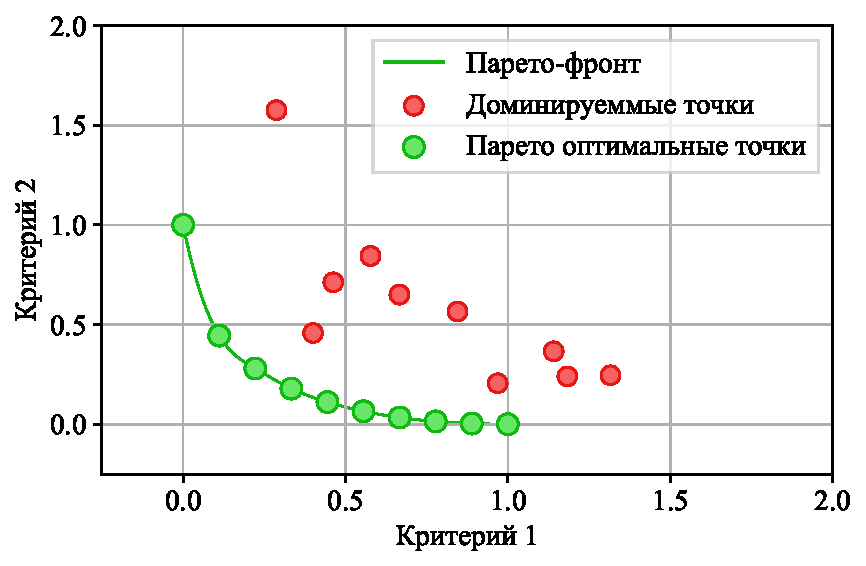
\includegraphics{part4/pareto_front_demonstrate.pdf}
    \caption{Пример фронта Парето для двух критериев.}\label{fig:pareto_front_example}
\end{figure}[ht]
На рисунке видно, что фронт Парето представляет собой кривую, состоящую из
недоминируемых решений
(точек), для которых невозможно улучшить один критерий без ухудшения другого.


Основные свойства оптимальности по Парето:
\begin{enumerate}
    \item Несравнимость: Парето-оптимальные решения несравнимы между собой в смысле доминирования.

    \item Иерархическая структура: Концепция Парето-оптимальности может быть расширена на случай иерархической оптимизации, где критерии имеют различные приоритеты.

    \item Инвариантность: Парето-оптимальные решения инвариантны относительно монотонных преобразований целевых функций.

    \item Выпуклость: Если все целевые функции выпуклы и допустимое множество выпукло, то множество Парето также выпукло.
\end{enumerate}

Для нахождения множества Парето-оптимальных решений в задачах многокритериальной оптимизации
используются специальные эволюционные алгоритмы. Эти методы работают с популяциями решений и
постепенно улучшают их, используя механизмы, подобные естественному отбору. Ниже описаны два из наиболее
известных алгоритмов для поиска Парето-оптимальных решений.

Сущществует множество методов для поиска Парето-оптимальных решений, однако наиболее
распространенными являются эволюционные алгоритмы, такие как NSGA-II и SPEA2.

NSGA-II — это один из самых популярных эволюционных алгоритмов для многокритериальной оптимизации. Его ключевые особенности:

\begin{enumerate}
    \item Сортировка по доминированию: На каждом шаге алгоритм делит популяцию на несколько уровней,
    исходя из степени доминирования решений. Те решения, которые не доминируются другими, попадают в
    первый уровень, остальные сортируются в соответствии с их степенью доминирования.

    \item Crowding Distance: NSGA-II использует метрику "crowding distance" для оценки плотности
    решений в области фронта Парето. Это помогает поддерживать разнообразие решений, предотвращая
    их слияние в одном месте.

    \item Операторы отбора, скрещивания и мутаций: Алгоритм применяет стандартные операторы
    генетического алгоритма для эволюции популяции — отбор лучших решений, скрещивание и мутацию
    для создания нового поколения.
\end{enumerate}

NSGA-II обеспечивает эффективное нахождение множества Парето-оптимальных решений,
а также хорошо сохраняет разнообразие решений вдоль фронта Парето \cite*{deb2001multi}.

SPEA2 — это улучшенная версия алгоритма SPEA, разработанная для повышения эффективности поиска недоминируемых решений. Основные улучшения SPEA2 включают:

\begin{enumerate}
    \item Архивирование решений: SPEA2 сохраняет архив недоминируемых решений на каждом шаге, что помогает гарантировать,
    что фронт Парето не будет потерян в процессе эволюции.

    \item Оценка решений: Каждый элемент популяции получает оценку на основе того,
    сколько решений он доминирует и насколько сильно доминируется сам. Эта оценка
    используется для выбора кандидатов для следующего поколения.

    \item Учет плотности решений: Подобно NSGA-II, SPEA2 учитывает плотность решений
    вблизи каждого кандидата, что помогает поддерживать разнообразие и улучшать
    распределение решений вдоль фронта Парето.
\end{enumerate}

SPEA2 продемонстрировал высокую производительность на сложных задачах многокритериальной
оптимизации и может эффективно находить множество недоминируемых решений \cite{zitzler2001spea2}.

В задаче оптимизации параметров управления пневматическим приводом концепция оптимальности
по Парето позволяет учесть множественные, зачастую противоречивые, критерии качества управления.
Например, минимизация времени переходного процесса и минимизация колличества переключений распределителей
могут находиться в конфликте друг с другом. Построение фронта Парето в этом случае
позволяет выявить множество оптимальных компромиссных решений и
предоставить лицу, принимающему решения, полную картину возможных вариантов.



\section{Методы построения сурогантных моделей}\label{sec:ch4/sec2}
Суррогатное моделирование является достаточно эффектиынвм методом в
задачах многокритериальной оптимизации, особенно при построении
Парето-фронта. Как правило, оно используется для аппроксимации сложных и вычислительно
затратных функций или систем, что позволяет значительно снизить временные и вычислительные
затраты на решение задач, требующих многократной оценки целевых функций. Данный
подход особенно полезен в тех случаях, когда каждая отдельная оценка целевой функции
является дорогостоящей с точки зрения времени или ресурсов, как это часто встречается
при численном моделировании физических процессов или компьютерных симуляциях сложных
инженерных систем.

Для синжения Для снижения вычислительных затрат используется суррогатное моделирование,
при котором сложные функции аппроксимируются с помощью более простых моделей,
называемых суррогатами, которые можно быстро и эффективно вычислять.
Это позволяет оптимизировать процесс поиска Парето-фронта и находить решения
с меньшими затратами ресурсов.



\subsection{Обзор методов суррогатного моделирования}\label{sec:ch4/sec2/subsec1}


\paragraph{Полиномиальная регрессия}\label{sec:ch4/sec2/subsec1/subsubsec1}

Полиномиальная регрессия представляет собой метод аппроксимации данных
с использозванием полиномов различных степеней. Этот метод является расширением линейной
регрессии и позволяет моделировать зависисмости между входными и выходными переменными более
гибким образом, используя дополнительные нелинейные термины, такие как квадратичные, кубические члены
и~т.д., а также их взаимодействия \cite{fan2018local}.

Полиномиальная регрессия предполагает, что зависимость между предикторами и откликом
можеты быть описана полиноминальной функцией вида:

\begin{equation*}
    \hat{y}(\mathbf{x}) = \beta_0 + \sum_{i=1}^{p} \beta_i x_i + \sum_{i=1}^{p} \sum_{j=1}^{p} \beta_{ij} x_i x_j + \ldots,
\end{equation*}
где $\hat{y}(\mathbf{x})$ -- предсказанное значение отклика;
$\beta_0$ -- свободный член (интерцепт);
$\beta_i$ -- коэффициенты линейных членов $x_i$;
$\beta_{ij}$ -- коэффициенты взаимодействия между переменными $x_i$ и $x_j$;
$p$ -- количество перменных;
$x_i,~x_j$ -- входные переменные.

Для случая квадратичной регрессии полиноминальная функция принимает вид:

\begin{equation*}
    \hat{y} = \beta_0 + \beta_1 x_1 + \beta_2 x_2 + \beta_3 x_1^2
    + \beta_4 x_2^2 + \beta_5 x_1 x_2.
\end{equation*}

Здесь учитываются коэффициенты линейных $\beta_1,~\beta_2$ и квадратичных $\beta_3,~\beta_4$ членов,
а также коэффициент взаимодействия $\beta_5$ \cite{heiberger2009polynomial}.

Для определения коэффициентов $\beta$ используется метод наименьших квадратов,
который минимизирует сумму квадратов отколнений между наблюдаемыми значениям $y_i$
и предсказанными $\hat{y}_i$. Задача оптимизации формулируется следующим образом:

\begin{equation*}
    \min_{\beta} \sum_{i=1}^{n} (y_i - \hat{y}_i)^2 =
    \min_{\beta} \sum_{i=1}^{n} \left\{
    y_i - \left(\beta_0 + \sum_{j=1}^{p} \beta_j x_{ij}
    + \sum_{j=1}^{p} \sum_{k=1}^{p} \beta_{jk} x_{ij} x_{ik}
    \right)
    \right\}^2,
\end{equation*}
где $n$ -- количество наблюдений.

Для решения этой задачи вводится матричная форма:

\begin{equation*}
    \mathbf{y} = \mathbf{X} \boldsymbol{\beta} + \boldsymbol{\epsilon},
\end{equation*}
где $\mathbf{y}$ -- вектор наблюдаемых значений откликов размерности $n \times 1$;
$\mathbf{X}$ -- матрица признаков размерности $n \times m$, где $m$ -- количество коэффициентов,
включая взаимодействия и нелинейные члены;
$\boldsymbol{\beta}$ -- вектор коэффициентов размерности $m \times 1$;
$\boldsymbol{\epsilon}$ -- вектор ошибок.

Оценка коэффицикнтов $\boldsymbol{\beta}$ производится с использованием псевдообратной матрицы:
\begin{equation*}
    \boldsymbol{\beta} = (\mathbf{X}^T \mathbf{X})^{-1} \mathbf{X}^T \mathbf{y}.
\end{equation*}
где $(\mathbf{X}^T \mathbf{X})^{-1} \mathbf{X}^T$ -- псевдообратная матрица Мура-Пенроуза,
которая обеспечивает минимизацию ошибки на оценке коэффициентов \cite{meyer2009matrix}.

Преимущества полиномиальной регрессии для задачи оптимизации управления электропневматическими приводами:
\begin{enumerate}
    \item Простота реализации и интерпретации модели.
    \item Низкие вычислительные затраты на построение и использование модели.
    \item Возможность аналитического вычисления градиентов, что полезно для оптимизационных алгоритмов.
\end{enumerate}

Ограничения метода:
\begin{enumerate}
    \item Ограниченная способность моделировать сложные нелинейные зависимости, характерные для пневматических систем;
    \item Риск переобучения при использовании полиномов высоких степеней;
    \item Чувствительность к выбросам в экспериментальных данных.
\end{enumerate}

\paragraph{Радиальные базисные функции}\label{sec:ch4/sec2/subsec1/subsubsec2}


Преимущества метода RBF для моделирования электропневматических приводов:

\begin{enumerate}
    \item Способность эффективно аппроксимировать сложные нелинейные зависимости.
    \item Хорошая обобщающая способность при правильном выборе параметров.
    \item Возможность точной интерполяции в экспериментальных точках.
\end{enumerate}

Ограничения метода:

\begin{enumerate}
    \item Чувствительность к выбору параметров (количество и расположение центров, тип базисной функции, параметр формы).
    \item Потенциальные проблемы с обусловленностью матрицы интерполяции при большом количестве базисных функций.
    \item Сложность интерпретации модели по сравнению с полиномиальной регрессией.
\end{enumerate}

\parapgaph{Гауссовы процессы (Кригинг)}\label{sec:ch4/sec2/subsec1/subsubsec3}

Кригинг (Гауссовы процессы) является мощным методом интерполяции,
который позволяет строить суррогатные модели для сложных функций,
используя концепцию случайных процессов \cite{gramacy2020surrogates}. Он основан
на предположении, что процесс \( y(\mathbf{x}) \) может быть представлен в виде:

\begin{equation*}
    y(\mathbf{x}) = \mu + Z(\mathbf{x}),
\end{equation*}
где $\mu$ -- среднее значение; $Z(\mathbf{x})$ -- гауссовский процесс с нулевым средним и
ковариационной функцией \cite{marrel2024probabilistic}:

\begin{equation*}
    \text{Cov}(Z(\mathbf{x}_i), Z(\mathbf{x}_j)) = k(\mathbf{x}_i, \mathbf{x}_j),
\end{equation*}

Ковариационная функция часто задается как радиальная базисная функция:

\begin{equation*}
    k(\mathbf{x}_i, \mathbf{x}_j) = \sigma^2 \exp\left(-\frac{\|\mathbf{x}_i - \mathbf{x}_j\|^2}{2l^2}\right),
\end{equation*}.
где \( \sigma^2 \) — дисперсия;
$l$ — параметр длины \cite{figueroa2021gaussian}.

Предсказание значений в новых точках $\mathbf{x}_*$ осуществляется через условное распределение, учитывающее известные значения.
Среднее предсказание и его дисперсия определяются как:

\begin{equation*}
    \hat{y}(\mathbf{x}_*) = \mu + \mathbf{k}_*^T \mathbf{K}^{-1} (\mathbf{y} - \mu \mathbf{1}_n),
\end{equation*}

\begin{equation*}
    \text{Var}(\hat{y}(\mathbf{x}_*)) = k(\mathbf{x}_*, \mathbf{x}_*) - \mathbf{k}_*^T \mathbf{K}^{-1} \mathbf{k}_*,
\end{equation*}
где $\mathbf{k}_*$ — вектор ковариаций между новой точкой и обучающими точками;
$\mathbf{K}$ — ковариационная матрица \cite{zhou2020enhanced}.

Кригинг широко применяется в задачах многокритериальной оптимизации и позволяет
не только предсказывать значения, но и оценивать их неопределенность, что особенно
полезно при построении фронтов Парето и выборе компромиссных решений \cite{radaideh2020surrogate}.

Преимущества метода кригинга для моделирования электропневматических приводов:

\begin{enumerate}
    \item Высокая точность интерполяции и экстраполяции;
    \item Возможность оценки неопределенности предсказаний;
    \item Гибкость в моделировании сложных нелинейных зависимостей;
    \item Эффективность при ограниченном количестве экспериментальных данных.
\end{enumerate}

Ограничения метода:

\begin{enumerate}
    \item Вычислительная сложность при большом количестве экспериментальных точек;
    \item Чувствительность к выбору функции корреляции и ее параметров;
    \item Сложность интерпретации модели по сравнению с детерминированными методами.
\end{enumerate}

\parapraph{Метод опорных векторов}\label{sec:ch4/sec2/subsec1/subsubsec4}

Метод опорных векторов (SVM) представляет собой один из наиболее эффективных методов классификации и
регрессии, основанный на поиске гиперплоскости, которая максимизирует зазор между классами.
Основная идея заключается в преобразовании исходных данных в более
высокое измерение с целью нахождения разделяющей гиперплоскости \cite{Jakkula2006}.

Рассмотрим обучающую выборку:
\begin{equation*}
    \{(x_i, y_i)\}_{i=1}^N,
\end{equation*}
где $x_i \in \mathbb{R}^n$ -- вектор признаков;
$y_i \in \{-1, 1\}$ -- метка класса.

Задача заключается в нахождении гиперплоскости,
которая разделяет два класса с максимальным зазором. Гиперплоскость определяется уравнением:

\begin{equation*}
    f(x) = w^T x + b = 0,
\end{equation*}
где $w \in \mathbb{R}^n$ -- вектор весов;
$b \in \mathbb{R}$ -- смещение.

Целью является минимизация следующей функции потерь с учетом ограничений:

\begin{equation*}
    \min_{w, b} \frac{1}{2} \|w\|^2,
\end{equation*}
при условиях:

\begin{equation*}
    y_i (w^T x_i + b) \geq 1, \quad i = 1, \ldots, N.
\end{equation*}

Для решения данной задачи применяется метод множителей Лагранжа,
что приводит к следующей двойственной задаче \cite{Patle2013}:

\begin{equation*}
    \max_{\alpha} \sum_{i=1}^N \alpha_i - \frac{1}{2} \sum_{i=1}^N \sum_{j=1}^N \alpha_i \alpha_j y_i y_j (x_i^T x_j),
\end{equation*}
при ограничениях:

\begin{equation*}
    \sum_{i=1}^N \alpha_i y_i = 0, \quad \alpha_i \geq 0, \quad i = 1, \ldots, N.
\end{equation*}
где $\alpha_i$ -- множители Лагранжа, которые определяют вклад каждого образца в решение задачи.

Для повышения мощности метода используется преобразование исходных данных
в пространство более высокой размерности с помощью ядровых
функций

\begin{equation*}
    K(x_i, x_j) = \phi(x_i)^T \phi(x_j),
\end{equation*}
где $\phi(\cdot)$ — отображение в новое
пространство признаков.

Распространенные ядра включают линейное,
полиномиальное и гауссово (радиальное базисное) ядро \cite{Deris2011}:

\begin{itemize}
    \item Линейное: $K(x_i, x_j) = x_i^T x_j$;
    \item Полиномиальное: $K(x_i, x_j) = (x_i^T x_j + 1)^d$;
    \item Гауссово: $K(x_i, x_j) = \exp\left(-\frac{\|x_i - x_j\|^2}{2\sigma^2}\right)$.
\end{itemize}

Для работы с шумными данными вводится параметр регуляризации $C$,
который контролирует баланс между шириной зазора и ошибками классификации.
Оптимизационная задача в этом случае принимает вид \cite{Boswell2002}:

\begin{equation*}
    \min_{w, b, \xi} \frac{1}{2} \|w\|^2 + C \sum_{i=1}^N \xi_i,
\end{equation*}

при условиях:

\begin{equation*}
    y_i (w^T x_i + b) \geq 1 - \xi_i, \quad \xi_i \geq 0, \quad i = 1, \ldots, N,
\end{equation*}
где $\xi_i$ -- переменные, отвечающие за допущенные ошибки.

Преимущества метода опорных векторов для построения суррогатной модели электропневматического привода:

\begin{enumerate}
    \item Высокая обобщающая способность, особенно при ограниченном наборе обучающих данных;
    \item Эффективность в задачах с большим количеством входных параметров;
    \item Способность моделировать сложные нелинейные зависимости.
\end{enumerate}

Ограничения метода:

\begin{enumerate}
    \item - Вычислительная сложность обучения модели для больших наборов данных;
    \item Чувствительность к выбору ядерной функции и настройке гиперпараметров;
    \item Сложность интерпретации модели по сравнению с более простыми методами, такими как полиномиальная регрессия.
\end{enumerate}

\paragraph{Нейронные сети}\label{sec:ch4/sec2/subsec1/subsubsec5}

\paragraph{Эволюционные алгоритмы и метаэвристики}\label{sec:ch4/sec2/subsec1/subsubsec6}
Эволюционные алгоритмы и метаэвристики представляют собой группу методов оптимизации,
вдохновленных природными процессами.
Они основанны на принципа биологической эвлюции и предлагают подходы, такие как генетические алгоритмы,
алгоритмы роя частиц, иммунные алгоритмы и др., которые позволяют эффективно искать решения
в пространстве возможных параметров \cite{zhang2015comparision}.

Основная идея эволюционных алгоритмов заключается в имитации процесса естественного отбора,
где популяция решений обновляется с каждым шагом алгоритма, и только наилучшие решения
сохраняются для следующего поколения. Алгоритм начинается с инициализации популяции случайных
решений, где каждое решение представляет собой набор параметров управления. Далее, для каждой
особи в популяции оценивается функция приспособленности, которая определяет, насколько хорошо
решение выполняет поставленную задачу. На основе функции приспособленности отбираются лучшие
решения, которые подвергаются мутации и скрещиванию, чтобы создать новые решения, и процесс
повторяется до тех пор, пока не будет достигнута заданная точность или не исчерпаны
вычислительные ресурсы.

Математически, решение $\mathbf{x}$ оптимизируется с помощью эволюционного алгоритма, следуюя
процедуре:

\begin{equation*}
    x^{t+1} = \text{ОТБОР} \left\{
    \text{МУТАЦИЯ} \left\{
    \text{СКРЕЩИВАНИЕ} \left\{
    x^t
    \right\}
    \right\}
    \right\},
\end{equation*}
где $x^t$ -- текущее решение;
$x^{t+1}$ -- новое решение;
$\text{ОТБОР}$ -- процедура отбора лучших решений или решений с высокой приспособленностью;
$\text{МУТАЦИЯ}$ -- процедура случайного или направленного изменения решения;
$\text{СКРЕЩИВАНИЕ}$ -- процедура комбинирования решений для создания новых вариантов.

Основные элементы эволюционного алгоритма можно описать следующим образом:

\begin{enumerate}
    \item Инициализация популяции: создание случайной популяции решений $x_i,~i = 1, \ldots, N$;
    \item Оценка приспособленности: для каждого решения рассчитвыается функция приспособленности $f(x_i)$,
          определяющая качество решения;
    \item Отбор: выбор лучших решений для создания нового решения;
    \item Скрещивание и мутация: создаются новые решения путем комбинирования и изменения существующих;
    \item Замена: новые решения заменяют старые в популяции и процесс повторяется до достижения критерия останова.
\end{enumerate}

Основные трудности применения эволюционных алгоритмов заключается
в определении параметров алгоритма, таких как размер популяции, вероятность мутации и
скрещивания, а также в обеспечении достаточной вычислительной мощности для
обработки большого числа итераций.

Метаэврестические подходы, такие как алгоритмы роя частиц и методы имитации отжига,
дополняют эволлюционные алгоритмы, предоставляя дополнительные инструменты для
исследования пространства решений. Эти методы доказали свою эффективность в
решении задач многокритериальной оптимизации, где необходимо сбалансировать
несколько противоречивых показателей качества.

Например, алгоритмы роя частиц (PSO) имитируют поведение стаци, где каждый
агент (частица) премещается в пространтсве решений с учетом своей собственной
истории и информации, полученной от других агентов. Частица $i$ обновляет
свою скорость и положение следующим образом:

\begin{equation*}
    \begin{aligned}
        v_i^{t+1} & = \omega \v_i^t + c_1 r_1 (p_i^t - x_i^t) + c_2 r_2 (g^t - x_i^t), \\
        x_i^{t+1} & = x_i^t + v_i^{t+1},
    \end{aligned}
\end{equation*}
где $\omega$ -- коэффициент инерции;
$c_1, c_2$ -- коэффициенты обучения;
$r_1, r_2$ -- случайные числа;
$p_i$ -- лучшее положение частицы;
$g$ -- лучшее положение частицы.

Данные методы позволяют эффективно находить компромисные решения в условиях
многокритериальной оптимизации, что делает их особенно полезными при
управлении пневмоприводами и другими сложными системами, где требуется балансировать
между различными критериями, такими как точность и частота переключеий.

Преимущества эволюционных алгоритмов и метаэвристик для моделирования электропневматических приводов:

\begin{enumerate}
    \item Способность находить компромисные решения в условиях многокритериальной оптимизации;
    \item Эффективность в поиске глобальных оптимумов в пространстве параметров;
    \item Легкость в адаптации для многокритериальной оптимизации, что позволяет учитывать
          различные критерии качества.
\end{enumerate}

Ограничения методов:
\begin{enumerate}
    \item Высокая вычислительная сложность при большом количестве параметров;
    \item Чувствительность к выбору параметров алгоритма;
    \item Нет гарантии нахождения глобального оптимума.
\end{enumerate}

\subsection{Выбор оптимального метода построения суррогатных моделей}\label{sec:ch4/sec2/subsec2}

В рамках исследования методов построения суррогатных моделей
для многокритериальной оптимизации алгоритмов управления
электропневматическими приводами с дискретными распределителями
был применен метод морфологического анализа Фрица Цвикки. Данный
метод позволяет систематически рассмотреть все возможные решения
проблемы путем анализа всех комбинаций параметров, что особенно важно
при выборе оптимального подхода в сложных многопараметрических задачах.

Метод Цвикки включает в себя несколько этапов. На первом этапе
формулируется проблема и определяются ключевые параметры,
характеризующие возможные решения. В нашем случае, ключевыми
параметрами для оценки методов построения суррогатных моделей были выбраны:

A. Способность к аппроксимации нелинейных зависимостей
B. Масштабируемость
C. Вычислительная эффективность
D. Интерпретируемость результатов
E. Способность к обобщению
F. Адаптивность к типам данных
G. Оценка неопределенности

Для каждого параметра были определены возможные значения:
низкое, среднее и высокое (или эквивалентные им).
Это позволяет создать морфологическую матрицу,
которая представляет собой многомерное пространство возможных решений.

\begin{table}[h]
    \centering
    \caption{Морфологическая матрица методов построения суррогатных моделей}
    \begin{tabular}{lccc}
        \midrule
        Параметр                          & Значение 1 & Значение 2 & Значение 3 \\
        \midrule
        A. Способность к аппроксимации    & Низкая     & Средняя    & Высокая    \\
        нелинейных зависимостей           &            &            &            \\

        B. Масштабируемость               & Плохая     & Средняя    & Хорошая    \\
        C. Вычислительная эффективность   & Низкая     & Средняя    & Высокая    \\
        D. Интерпретируемость результатов & Низкая     & Средняя    & Высокая    \\
        E. Способность к обобщению        & Низкая     & Средняя    & Высокая    \\
        F. Адаптивность к типам данных    & Низкая     & Средняя    & Высокая    \\
        G. Оценка неопределенности        & Нет        & Частичная  & Полная     \\
        \midrule
    \end{tabular}
    \label{tab:morphological_matrix}
\end{table}

На следующем этапе анализа каждый рассматриваемый метод
построения суррогатных моделей был оценен по каждому параметру.
Оценка проводилась на основе теоретических свойств методов и опыта
их применения в схожих задачах. Результаты оценки представлены в следующей таблице:

\begin{table}[h]
    \centering
    \caption{Оценка методов по параметрам}
    \begin{tabular}{l|c|c|c|c|c|c|c}
        \midrule
        Метод                             & A & B & C & D & E & F & G \\
        \midrule
        Полиномиальная регрессия          & 1 & 1 & 3 & 3 & 1 & 1 & 1 \\
        \hline
        Радиальные базисные функции (RBF) & 2 & 2 & 2 & 2 & 2 & 2 & 1 \\
        \hline
        Кригинг (Гауссовы процессы)       & 2 & 1 & 1 & 1 & 3 & 2 & 3 \\
        \hline
        Метод опорных векторов (SVM)      & 2 & 3 & 2 & 1 & 3 & 2 & 1 \\
        \hline
        Нейронные сети                    & 3 & 3 & 2 & 1 & 3 & 3 & 2 \\
        \hline
        Эволюционные алгоритмы            & 3 & 2 & 1 & 2 & 2 & 3 & 1 \\
        \midrule
    \end{tabular}
    \label{tab:method_evaluation}
\end{table}

Здесь числовые значения соответствуют оценкам из
морфологической матрицы (1 - низкая/плохая, 2 - средняя, 3 - высокая/хорошая).

Для наглядного представления результатов анализа на рисунке \ref{fig:morphological_analysis}
была приведена лепестковая диаграмма, отражающая оценки методов по каждому из
рассмотренных параметров.

\begin{figure}[ht]
    \centerfloat{
        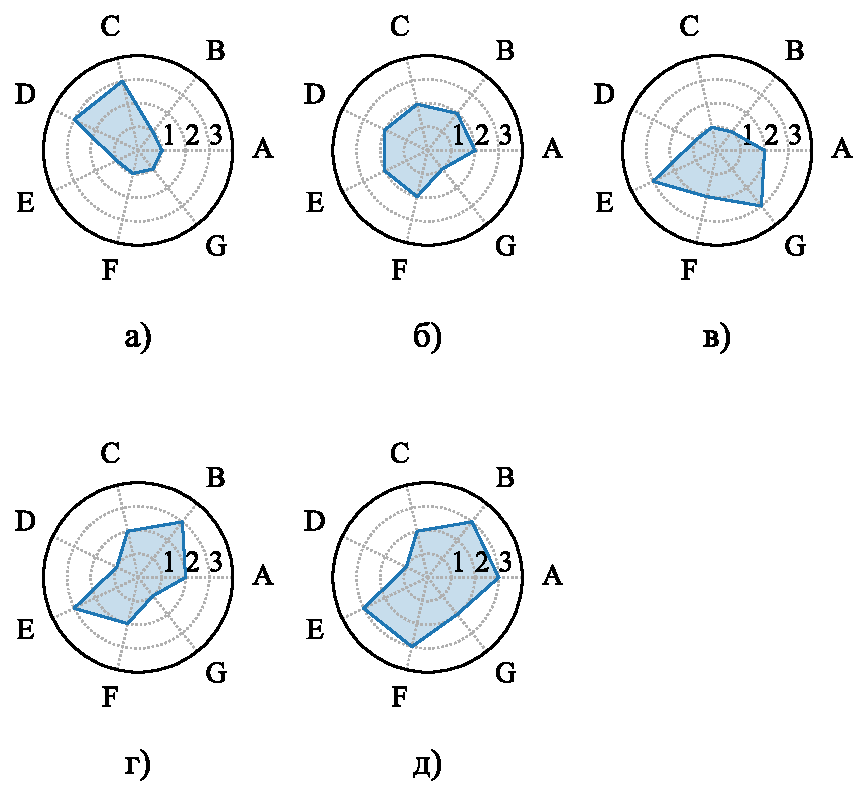
\includegraphics{part4/morphological_analyse.pdf}
    }
    \caption{Лепестковые диаграммы каждого варианта}\label{fig:morphological_analysis}
\end{figure}

Для выбора оптимального метода необходимо учитывать важность
каждого параметра в контексте нашей конкретной задачи.
Учитывая специфику многокритериальной оптимизации алгоритмов
управления электропневматическими приводами с дискретными
распределителями, были присвоены следующие веса параметрам:

\begin{itemize}
    \item A: 0.25 -- высокая важность из-за нелинейности системы;
    \item B: 0.20 -- важно для работы с множеством параметров;
    \item C: 0.15 -- важно для итеративного процесса оптимизации;
    \item D: 0.05 -- менее важно для данной задачи;
    \item E: 0.20 -- важно для работы с новыми комбинациями параметров;
    \item F: 0.10 -- важно для работы с различными типами параметров;
    \item G: 0.05 -- менее важно для данной задачи.
\end{itemize}

Используя эти веса, была вычислена взвешенная сумма для каждого метода. Рассмотрим пример расчета взвешенной суммы для метода нейронных сетей:

\begin{equation}
    \begin{split}
        S_{НС} = & 0.25 \cdot 3 + 0.20 \cdot 3 + 0.15 \cdot 2 + 0.05 \cdot 1 + \\
        +        & 0.20 \cdot 3 + 0.10 \cdot 3 + 0.05 \cdot 2 =                \\
        =        & 0.75 + 0.60 + 0.30 + 0.05 + 0.60 + 0.30 + 0.10 =            \\
        =        & 2.60
    \end{split}
\end{equation}
где $S_{НС}$ -- взвешенная сумма для нейронных сетей, а числовые значения
соответствуют оценкам из таблицы \ref{tab:method_evaluation}.

Аналогичным образом были рассчитаны взвешенные суммы для остальных методов.
Результаты представлены в таблице \ref{tab:weighted_scores}.

\begin{table}[h]
    \centering
    \caption{Взвешенные оценки методов}
    \begin{tabular}{lc}
        \midrule
        Метод                             & Взвешенная сумма \\
        \midrule
        Полиномиальная регрессия          & 1.60             \\
        Радиальные базисные функции (RBF) & 1.95             \\
        Кригинг (Гауссовы процессы)       & 1.90             \\
        Метод опорных векторов (SVM)      & 2.25             \\
        Нейронные сети                    & 2.60             \\
        Эволюционные алгоритмы            & 2.15             \\
        \hline
    \end{tabular}
    \label{tab:weighted_scores}
\end{table}



Как видно из результатов, нейронные сети получили наивысшую взвешенную оценку
(2.60). Это объясняется тем, что они имеют высокие оценки по наиболее важным
критериям: способности к аппроксимации нелинейных зависимостей (вес 0.25),
масштабируемости (вес 0.20) и способности к обобщению (вес 0.20). Несмотря на
относительно низкую оценку по интерпретируемости результатов (1 с весом 0.05),
это не оказало значительного влияния на общий результат из-за низкого веса этого
критерия для нашей задачи.

На основе проведенного морфологического анализа с использованием метода
Цвикки, наиболее подходящим методом для построения суррогатной модели
в контексте многокритериальной оптимизации алгоритмов управления
электропневматическими приводами с дискретными распределителями
являются нейронные сети. Они получили наивысшую взвешенную оценку
благодаря своим сильным сторонам: высокой способности к аппроксимации
сложных нелинейных зависимостей, хорошей масштабируемости и работе с
высокоразмерными данными, высокой способности к обобщению и высокой
адаптивности к различным типам данных.

Несмотря на некоторые недостатки, такие как относительно низкая интерпретируемость
результатов и средняя вычислительная эффективность,
преимущества нейронных сетей в контексте данной задачи перевешивают
их недостатки. Для минимизации этих недостатков могут быть применены методы
регуляризации, техники визуализации и интерпретации нейронных сетей, а
также оптимизация архитектуры сети для повышения вычислительной эффективности.

\section{Разработка нейросетевой суррогатной модели}\label{sec:ch4/sec3}
В рамках разработки нейросетевой суррогатной модели для многокритериальной
оптимизации алгоритмов управления электропневматическими приводами была предложена
архитектура, основанная на концепции остаточных блоков. Данный подход позволяет
эффективно обучать глубокие сети, преодолевая проблему затухающих градиентов.
Структура модели включает входной слой, принимающий вектор параметров настройки
алгоритма управления, последовательность остаточных блоков и выходной линейный слой,
предсказывающий значения критериев качества управления.

Для повышения обобщающей способности модели и снижения
риска переобучения применяется техника регуляризации.
Процесс разработки суррогатной модели включал в себя оптимизацию
гиперпараметров, таких как количество остаточных блоков, размерности
скрытых слоев и скорость обучения, с использованием байесовской оптимизации.
Данный подход позволил создать эффективную суррогатную модель, способную
точно аппроксимировать сложные нелинейные зависимости между параметрами
алгоритма управления и критериями качества электропневматического привода.

\subsection{Архитектура модели}\label{sec:ch4/sec3/subsec1}

В целях повышения эффективности и точности суррогатного моделирования была разработана нейронная сеть,
основанная на архитектуре с использованием остаточных блоков (Residual Blocks). Данная архитектура была
выбрана для обеспечения устойчивости обучения и возможности построения глубоких моделей, способных захватывать
сложные нелинейные зависимости между входными параметрами и выходными метриками системы.

\paragraph{Структура нейронной сети}\label{sec:ch4/sec3/subsec1/subsubsec1}

Разработанная нейронная сеть представляет собой глубокую многослойную перцептронную модель (Multilayer Perceptron, MLP) \cite*{goodfellow2016deep},
интегрированную с остаточными блоками для улучшения процесса обучения и повышения обобщающей способности модели.
Архитектура сети состоит из следующих компонентов:

\begin{enumerate}
    \item Входной слой: входной слой принимает вектор признаков $\mathbf{x} \in \mathbb{R}^n$,
          представляющий праметры инициализации системы. В данном случае -- это парметры,
          которые изменяются в процессе оптимизации алгоритма. Колличестов нейронов во входном
          слое соответствует размерности входного вектора $n$;

    \item Последовательность остаточных блоков: основная часть сети состоит из серии остаточных блоков,
          каждый из которых включает в себя два линейных слоя с последующей нормализацией батча \cite*{ioffe2015batch},
          функцией активации ReLU и Dropout для регуляризации. Остаточные блоки
          реализуются для обеспечения прямого прохождения градиентов и предотвращения
          проблем, связанных с обучением глубоких сетей, таких как исчезающие градиенты \cite*{he2016deep}.

    \item Финальный линейный слой: После последовательности остаточных блоков добавляется финальный линейный слой,
          количество нейронов которого соответствует размерности выходных метрик $m$.
          Этот слой отвечает за преобразование скрытых представлений в предсказания модели.
\end{enumerate}

Рассмотрим каждый элемент архитектуры подробнее.
Фундаментальным структурным элементом данной сети является остаточный блок,
математическое описание которого может быть представлено следующим образом:

\begin{equation*}
    \mathbf{y} = F(\mathbf{x}, \{\mathbf{W}_i\}) + h(\mathbf{x}),
\end{equation*}
где $F(\mathbf{x}, {\mathbf{W}_i})$ -- остаточную функцию;
$h(\mathbf{x})$ -- функцию тождественного отображения или линейного проецирования.

Детализируя структуру остаточного блока,
можно выразить $F(\mathbf{x}, {\mathbf{W}_i})$ как композицию нескольких операций:

\begin{equation*}
    \begin{split}
        \mathbf{z}_1                    & = \sigma(\mathbf{W}_1\mathbf{x} + \mathbf{b}_1), \\
        \mathbf{z}_2                    & = D(\mathbf{z}_1, p),                            \\
        \mathbf{z}_3                    & = \mathbf{W}_2\mathbf{z}_2 + \mathbf{b}_2,       \\
        F(\mathbf{x}, \{\mathbf{W}_i\}) & = \mathbf{z}_3.
    \end{split}
\end{equation*}
где $\mathbf{W}_1, \mathbf{W}_2 \in \mathbb{R}^{m \times n}$ -- весовые матрицы;
$\mathbf{b}_1, \mathbf{b}_2 \in \mathbb{R}^m$ -- векторы смещения;
$\sigma(\cdot)$ -- функция активации ReLU;
$D(\cdot, p)$ -- операция dropout с вероятностью $p$.

Функция активации ReLU определяется как \cite*{nair2010rectified}:
\begin{equation*}
    \sigma(x) = \max(0, x).
\end{equation*}

Механизм dropout представляет собой эффективный метод регуляризации \cite*{srivastava2014dropout},
широко применяемый в глубоких нейронных сетях для предотвращения переобучения
и повышения их обобщающей способности. В контексте рассматриваемой суррогатной
модели, dropout играет ключевую роль в обеспечении надежности
и устойчивости предсказаний.

Сущность метода dropout заключается в случайном "выключении" определенной
доли нейронов в процессе обучения. Математически этот процесс может быть описан
следующим образом:

\begin{equation*}
    \tilde{\mathbf{z}} = \mathbf{m} \odot \mathbf{z},
\end{equation*}
где $\mathbf{z} \in \mathbb{R}^n$ -- вектор активаций нейронов;
$\mathbf{m} \in {0, 1}^n$ -- бинарная маска dropout;
$\tilde{\mathbf{z}}$ -- результирующий вектор после применения dropout.

Элементы маски $\mathbf{m}$ генерируются независимо из распределения Бернулли с параметром $1-p$:

\begin{equation*}
    m_i \sim \text{Bernoulli}(1-p), \quad i = 1, \ldots, n,
\end{equation*}
где $p$ -- вероятность "выключения" нейрона, являющуюся одним из гиперпараметров модели.

Значение $1-p$, соответственно, определяет вероятность сохранения нейрона активным.

Применение dropout приводит к тому, что математическое
ожидание выходного значения каждого нейрона уменьшается в $1-p$ раз:

\begin{equation*}
    \mathbb{E}[\tilde{z}_i] = (1-p)z_i.
\end{equation*}

Для компенсации данного эффекта во время обучения, выход нейрона
корректируется путем масштабирования на $1/(1-p)$:

\begin{equation}
    \tilde{\mathbf{z}} = \frac{1}{1-p}\mathbf{m} \odot \mathbf{z}.
\end{equation}

Важно отметить, что на этапе инференса (применения обученной модели)
dropout не используется. Это эквивалентно использованию математического ожидания активаций:

\begin{equation}
    \mathbf{z}_{\text{test}} = \mathbb{E}[\tilde{\mathbf{z}}] = \mathbf{z}.
\end{equation}

Применение dropout в остаточном блоке суррогатной модели может быть выражено следующим образом:

\begin{equation*}
    \begin{split}
        \mathbf{z}_1         & = \sigma(\mathbf{W}_1\mathbf{x} + \mathbf{b}_1)                                             \\
        \tilde{\mathbf{z}}_1 & = \frac{1}{1-p}\mathbf{m} \odot \mathbf{z}_1, \quad \mathbf{m}_i \sim \text{Bernoulli}(1-p) \\
        \mathbf{z}_2         & = \mathbf{W}_2\tilde{\mathbf{z}}_1 + \mathbf{b}_2
    \end{split}
\end{equation*}
где $\sigma(\cdot)$ обозначает функцию активации;
$\mathbf{W}_1$ и $\mathbf{W}_2$ -- весовые матрицы;
$\mathbf{b}_1$ и $\mathbf{b}_2$ -- векторы смещения.

Остаточные блоки объединяются в последовательность, образуя глубокую модель, способную
захватывать сложные нелинейные зависимости между входными параметрами и выходными метриками
качества управления электропневматическим приводом.

\subsection{Процесс обучения}\label{sec:ch4/sec3/subsec2}
\subsection{Оптимизация гиперпараметров}\label{sec:ch4/sec3/subsec3}

\section{Алгоритм построения фронта Парето}\label{sec:ch4/sec4}
\subsection{Генерация начальной выборки методом латинского гиперкуба}\label{sec:ch4/sec4/subsec1}
\subsection{Обучение ансамбля нейронных сетей}\label{sec:ch4/sec4/subsec2}
\subsection{Генерация и отбор Парето-оптимальных решений}\label{sec:ch4/sec4/subsec3}

\section{Визуализация и анализ фронта Парето}\label{sec:ch4/sec5}
\subsection{Методы визуализации многомерных фронтов Парето}\label{sec:ch4/sec5/subsec1}
\subsection{Метрики сравнения фронтов Парето}\label{sec:ch4/sec5/subsec2}
\subsection{Анализ чувствительности и робастности решений}\label{sec:ch4/sec5/subsec3}
           % Глава 4
\chapter{СРАВНИТЕЛЬНЫЙ АНАЛИЗ МЕТОДОВ УПРАВЛЕНИЯ ЭЛЕКТРОПНЕВМАТИЧЕСКИМ ПРИВОДОМ С ДИСКРЕТНЫМ УПРАВЛЕНИЕМ}\label{ch:ch6}

\section{Анализ эффективности алгоритмов по экспериментальным данным}\label{sec:ch6/sec1}

\section{Построение фронтов Парето для алгоритмов управления}\label{sec:ch6/sec2}

\section{Сравнительные анализ фронтов Парето}\label{sec:ch6/sec3}

\section{Оценка робастности алгоритмов управления}\label{sec:ch6/sec4}

\section{рекомендации по выбору алгоритма управления для различных условий эксплуатации}\label{sec:ch6/sec5}

           % Глава 5
\chapter*{Заключение}                       % Заголовок
\addcontentsline{toc}{chapter}{Заключение}  % Добавляем его в оглавление

%% Согласно ГОСТ Р 7.0.11-2011:
%% 5.3.3 В заключении диссертации излагают итоги выполненного исследования, рекомендации, перспективы дальнейшей разработки темы.
%% 9.2.3 В заключении автореферата диссертации излагают итоги данного исследования, рекомендации и перспективы дальнейшей разработки темы.
%% Поэтому имеет смысл сделать эту часть общей и загрузить из одного файла в автореферат и в диссертацию:

%% Согласно ГОСТ Р 7.0.11-2011:
%% 5.3.3 В заключении диссертации излагают итоги выполненного исследования, рекомендации, перспективы дальнейшей разработки темы.
%% 9.2.3 В заключении автореферата диссертации излагают итоги данного исследования, рекомендации и перспективы дальнейшей разработки темы.
В результате проведенного диссертационного исследования достигнута поставленная
цель комплексного повышения статико-динамических и ресурсных показателей позиционного пневмопривода с
дискретными распределителями в условиях их конфликтности. Получены следующие основные результаты:

\begin{enumerate}
    \item Разработана комплексная математическая модель позиционного пневмопривода с дискретными распределителями,
    которая включает в себя как силовую, так и управляющую структуры. Модель учитывает нелинейные термодинамические
    процессы в полостях пневмоцилиндра, переменную структуру системы при переключении распределителей, а также
    динамические эффекты сухого и вязкого трения. Высокая степень согласованности результатов моделирования с
    экспериментальными данными (расхождение не превышает 5~--~7\%) подтверждает адекватность и достоверность
    разработанной модели для решения задач анализа и синтеза пневмоприводов различной структуры.

    \item Проведен комплексный анализ различных структур пневмопривода, что позволило выявить оптимальные
    режимы переключения распределителей при позиционировании рабочего органа. Разработаны структуры управления
    на основе различных принципов: модифицированная структура ПИД-регулятора с блоком прогнозирования тормозного пути,
    управление в скользящих режимах с интегральной и терминальной поверхностями, нечеткое управление и прогнозное управление.
    Экспериментальный анализ подтвердил, что прогнозное управление обеспечивает повышение точности позиционирования на 25~--~30\%
    при одновременном сокращении числа переключений распределителей на 35~--~45\% по сравнению с традиционными алгоритмами.

    \item Проведен натурный эксперимент на специально разработанном лабораторном стенде, который подтвердил работоспособность
    предложенных структур и высокую достоверность результатов, полученных с использованием разработанной математической модели.
    Сравнительный анализ экспериментальных данных показал, что наибольшую точность моделирования демонстрируют алгоритмы прогнозного
    управления и семирежимного управления в скользящих режимах, где средняя относительная ошибка не превышает 4,65\%.
    Расхождение между расчетными и экспериментальными данными по основным показателям качества составляет
    не более 7\% для всех исследованных алгоритмов управления.

    \item Разработана методика многокритериального структурно-параметрического синтеза, основанная
    на использовании фронтов Парето с применением замещающей суррогатной нейросетевой модели. Для
    формирования обучающей выборки применен метод латинского гиперкуба, обеспечивающий оптимальное
    заполнение пространства параметров, что позволило сократить вычислительные затраты при построении
    фронтов Парето на 48\%. Использование суррогатной модели обеспечило среднюю точность аппроксимации 91\%
    при максимальном отклонении 12\%.

    \item Определена взаимосвязь между конфликтными статико-динамическими и ресурсными показателями
    для позиционных пневмоприводов различной структуры на основе анализа фронтов Парето. Установлено,
    что для ПИД-регулятора с ШИМ диапазон изменения критерия $ITAE$ составляет от 0,0298 до 0,0427 \si{\meter\per\second\square}
    при изменении точности от 0,41 до 2,57 мм. Семирежимное управление с интегральной поверхностью
    обеспечивает точность 0,13 мм при $ITAE = 0,019$ \si{\meter\per\second\square} и $SI = 15$, а прогнозное управление демонстрирует
    точность 0,12 мм при $ITAE = 0,032$ \si{\meter\per\second\square} и $SI = 14$~--~$16$. Для нечеткого регулятора характерны
    наилучшие показатели по критерию динамической эффективности ($ITAE = 0,006$ \si{\meter\per\second\square}) при точности 0,40 мм.

    \item Сформированы практические рекомендации по выбору оптимальной структуры позиционного
    пневмопривода с дискретными распределителями. Выделены четыре предпочтительные области
    применения различных алгоритмов управления:
    \begin{itemize}
        \item область высоконагруженных систем (УСР-И-5, MPC) с точностью 0,12~--~0,36 мм;
        \item область точных манипуляторов (УСР-И-7) с точностью 0,14 мм;
        \item область промышленной автоматики (УСР-Т-5, УСР-Т-7) с точностью 0,13~--~0,28 мм;
        \item область простых систем (ПИД+ШИМ, УСР-И-3) с точностью 0,5~--~2,5 мм.
    \end{itemize}
    Определены рекомендуемые значения параметров алгоритмов управления для типовых задач
    позиционирования, что позволяет сократить сроки проектирования и повышает эффективность разрабатываемых систем.
\end{enumerate}

Полученные результаты позволяют на научной основе выбирать оптимальную структуру и
параметры позиционного пневмопривода с дискретными распределителями в зависимости
от конкретных требований, существенно сокращая сроки проектирования и повышая
эффективность разрабатываемых систем.
      % Заключение
\include{Dissertation/acronyms}        % Список сокращений и условных обозначений
\chapter*{Словарь терминов}             % Заголовок
\addcontentsline{toc}{chapter}{Словарь терминов}  % Добавляем его в оглавление

\textbf{Адиабатический процесс} : термодинамический процесс, происходящий без теплообмена системы с окружающей средой.

\textbf{Векторное поле} : математический объект, описывающий направления и интенсивность движения системы в фазовом пространстве.

\textbf{Горизонт прогноза} : интервал времени в будущем, на который выполняется прогнозирование поведения системы в методе прогнозного управления.

\textbf{Горизонт управления} : количество шагов управляющих воздействий, оптимизируемых одновременно в методе прогнозного управления.

\textbf{Гистерезис} : явление, при котором физическая система неоднозначно зависит от своей предыстории (выходная величина зависит не только от входной, но и от предыдущего состояния системы).

\textbf{Дефаззификация} : процесс преобразования нечеткого множества или нечеткой величины в четкое (конкретное) значение.

\textbf{Закон Сен-Венана--Ванцеля} : закон, описывающий расход газа через отверстие или канал в зависимости от отношения давлений.

\textbf{Запирание полости} : состояние, при котором все распределители, соединенные с полостью пневмопривода, закрыты, что приводит к изоляции этой полости от системы питания и атмосферы.

\textbf{Интенсивность переключений} : критерий оптимизации, характеризующий частоту и количество переключений распределителей за цикл работы.

\textbf{Колебательность} : характеристика системы, отражающая склонность к осцилляциям вокруг положения равновесия.

\textbf{Критическое отношение давлений} : пороговое значение отношения давлений, при котором происходит переход от докритического к закритическому течению газа.

\textbf{Лингвистическая переменная} : переменная, значениями которой являются не числа, а слова или предложения естественного или формального языка.

\textbf{Метод центра тяжести} : способ дефаззификации в нечеткой логике, при котором четкое значение определяется как центр тяжести площади под кривой результирующей функции принадлежности.

\textbf{Многокритериальная оптимизация} : процесс нахождения решения, оптимального сразу по нескольким противоречивым критериям.

\textbf{Многорежимное управление} : подход к управлению, при котором система имеет несколько различных режимов работы с возможностью переключения между ними.

\textbf{Поверхность скольжения} : многообразие в пространстве состояний, определяющее динамику системы при управлении в скользящих режимах.

\textbf{Прогнозная модель} : упрощенная математическая модель объекта, используемая для прогнозирования его будущего поведения в прогнозном управлении.

\textbf{Парето-оптимальность} : состояние системы, при котором улучшение по одному критерию невозможно без ухудшения по другому критерию.

\textbf{Парето-фронт} : множество всех Парето-оптимальных решений в пространстве критериев оптимизации.

\textbf{Переменная структура} : свойство системы, при котором её структура (или закон управления) меняется в зависимости от состояния системы.

\textbf{Перерегулирование} : явление, при котором выходная величина системы превышает установившееся значение при переходном процессе.

\textbf{Политропный процесс} : термодинамический процесс, при котором теплоемкость системы остается постоянной.

\textbf{Пространство состояний} : математическое пространство, где каждая точка однозначно определяет состояние динамической системы.

\textbf{Расходная функция} : функция, описывающая зависимость массового расхода через дросселирующее устройство от отношения давлений.

\textbf{Релейная система} : система управления, в которой управляющее воздействие может принимать только дискретные значения.

\textbf{Режим торможения} : специальный режим работы пневмопривода, направленный на эффективное снижение скорости движения.

\textbf{Скользящий режим} : режим движения системы вдоль заданной поверхности переключения в пространстве состояний системы.

\textbf{Статическая ошибка} : ошибка, возникающая в системе автоматического управления в установившемся режиме работы.

\textbf{Суррогатное моделирование} : метод создания быстрых приближенных моделей сложных систем для использования в задачах оптимизации.

\textbf{Терм} : элемент терм-множества лингвистической переменной, представляющий определенное значение этой переменной.

\textbf{Термодинамический процесс} : изменение состояния термодинамической системы, сопровождающееся изменением ее термодинамических параметров.

\textbf{Терминальная поверхность} : тип поверхности скольжения, обеспечивающий достижение целевого состояния за конечное время.

\textbf{Трение LuGre} : модель трения, учитывающая микроскопические деформации контактирующих поверхностей, эффект Штрибека и вязкое трение.

\textbf{Уравнение Максвелла} : дифференциальное уравнение, связывающее изменение термодинамических функций состояния с изменением параметров системы.

\textbf{Упреждающее управление} : стратегия управления, при которой управляющее воздействие формируется с учетом прогноза будущего поведения системы.

\textbf{Фазовый портрет} : графическое представление траекторий динамической системы в фазовой плоскости или фазовом пространстве.

\textbf{Фазовое пространство} : пространство, образованное совокупностью всех возможных состояний динамической системы.

\textbf{Фаззификация} : процесс преобразования четких (конкретных) значений в степени принадлежности к нечетким множествам.

\textbf{Фронт Парето} : множество всех недоминируемых решений в задаче многокритериальной оптимизации.

\textbf{Функция принадлежности} : функция, определяющая степень принадлежности элемента к нечеткому множеству.

\textbf{Эффект Дала} : микроскопическое смещение объекта до начала макроскопического движения, учитываемое в моделях трения.

\textbf{Эффективная площадь} : условная площадь проходного сечения распределителя, используемая для расчета массового расхода.

\textbf{Эвристический алгоритм} : приближенный метод решения задач, не гарантирующий нахождение оптимального решения, но дающий приемлемое решение за разумное время.
%\textbf{AC} : accuracy -- критерий точности позиционирования, определяемый как модуль ошибки в установившемся режиме.
%\textbf{BDF} : backward Differential Formula -- метод обратных дифференциальных формул для численного решения жестких систем дифференциальных уравнений.
%\textbf{ITAE} : integral Time Absolute Error -- интегральный критерий качества переходного процесса с учетом времени.
%\textbf{MPC} : model Predictive Control — прогнозное управление с использованием модели объекта.
%\textbf{ПИД} : пропорционально-интегрально-дифференциальный (регулятор) -- тип регулятора, использующий трехкомпонентный закон управления.
%\textbf{РО} : рабочий орган -- исполнительный механизм, непосредственно выполняющий технологические операции.
%\textbf{SI} : switching Intensity -- критерий интенсивности переключений распределителей.
%\textbf{УСР-И-3} : управление в скользящих режимах с интегральной поверхностью с тремя режимами работы.
%\textbf{УСР-И-5} : управление в скользящих режимах с интегральной поверхностью с пятью режимами работы.
%\textbf{УСР-И-7} : управление в скользящих режимах с интегральной поверхностью с семью режимами работы.
%\textbf{УСР-Т-3} : управление в скользящих режимах с терминальной поверхностью с тремя режимами работы.
%\textbf{УСР-Т-5} : управление в скользящих режимах с терминальной поверхностью с пятью режимами работы.
%\textbf{УСР-Т-7} : управление в скользящих режимах с терминальной поверхностью с семью режимами работы.
%\textbf{ШИМ} : широтно-импульсная модуляция -- способ управления мощностью путем изменения скважности импульсов постоянной частоты.
      % Словарь терминов
\include{Dissertation/references}      % Список литературы
\include{Dissertation/lists}           % Списки таблиц и изображений (иллюстративный материал)

\setcounter{totalchapter}{\value{chapter}} % Подсчёт количества глав

%%% Настройки для приложений
\appendix
% Оформление заголовков приложений ближе к ГОСТ:
\setlength{\midchapskip}{20pt}
\renewcommand*{\afterchapternum}{\par\nobreak\vskip \midchapskip}
\renewcommand\thechapter{\Asbuk{chapter}} % Чтобы приложения русскими буквами нумеровались

\chapter{ОБЗОР МЕТОДОВ СУРРОГАТНОГО МОДЕЛИРОВАНИЯ}\label{chap:surrogate-modeling}

Суррогатные модели используются в качестве замены исходной модели для снижения трудоемкости
расчетов. В качестве таких моделей могут использоваться полиноминальная регрессия, радиальные
базисные функции и т.д. Ниже представлен обзор основных методов.

\paragraph{Полиномиальная регрессия}

Полиномиальная регрессия представляет собой метод аппроксимации данных
с использозванием полиномов различных степеней. Этот метод является расширением линейной
регрессии и позволяет моделировать зависисмости между входными и выходными переменными более
гибким образом, используя дополнительные нелинейные термины, такие как квадратичные, кубические члены
и~т.д., а также их взаимодействия \cite{fan2018local}.

Полиномиальная регрессия предполагает, что зависимость между предикторами и откликом
можеты быть описана полиноминальной функцией вида:

\begin{equation}
	\hat{y}(\mathbf{x}) = \beta_0 + \sum_{i=1}^{p} \beta_i x_i + \sum_{i=1}^{p} \sum_{j=1}^{p} \beta_{ij} x_i x_j + \ldots,
\end{equation}
где $\hat{y}(\mathbf{x})$ -- предсказанное значение отклика;
$\beta_0$ -- свободный член (интерцепт);
$\beta_i$ -- коэффициенты линейных членов $x_i$;
$\beta_{ij}$ -- коэффициенты взаимодействия между переменными $x_i$ и $x_j$;
$p$ -- количество перменных;
$x_i,~x_j$ -- входные переменные.

Для случая квадратичной регрессии полиноминальная функция принимает вид:

\begin{equation}
	\hat{y} = \beta_0 + \beta_1 x_1 + \beta_2 x_2 + \beta_3 x_1^2
	+ \beta_4 x_2^2 + \beta_5 x_1 x_2.
\end{equation}

Здесь учитываются коэффициенты линейных $\beta_1,~\beta_2$ и квадратичных $\beta_3,~\beta_4$ членов,
а также коэффициент взаимодействия $\beta_5$ \cite{heiberger2009polynomial}.

Для определения коэффициентов $\beta$ используется метод наименьших квадратов,
который минимизирует сумму квадратов отколнений между наблюдаемыми значениям $y_i$
и предсказанными $\hat{y}_i$. Задача оптимизации формулируется следующим образом:

\begin{equation}
	\min_{\beta} \sum_{i=1}^{n} (y_i - \hat{y}_i)^2 =
	\min_{\beta} \sum_{i=1}^{n} \left\{
	y_i - \left(\beta_0 + \sum_{j=1}^{p} \beta_j x_{ij}
	+ \sum_{j=1}^{p} \sum_{k=1}^{p} \beta_{jk} x_{ij} x_{ik}
	\right)
	\right\}^2,
\end{equation}
где $n$ -- количество наблюдений.

Для решения этой задачи вводится матричная форма:

\begin{equation}
	\mathbf{y} = \mathbf{X} \boldsymbol{\beta} + \boldsymbol{\epsilon},
\end{equation}
где $\mathbf{y}$ -- вектор наблюдаемых значений откликов размерности $n \times 1$;
$\mathbf{X}$ -- матрица признаков размерности $n \times m$, где $m$ -- количество коэффициентов,
включая взаимодействия и нелинейные члены;
$\boldsymbol{\beta}$ -- вектор коэффициентов размерности $m \times 1$;
$\boldsymbol{\epsilon}$ -- вектор ошибок.

Оценка коэффицикнтов $\boldsymbol{\beta}$ производится с использованием псевдообратной матрицы:
\begin{equation}
	\boldsymbol{\beta} = (\mathbf{X}^T \mathbf{X})^{-1} \mathbf{X}^T \mathbf{y}.
\end{equation}
где $(\mathbf{X}^T \mathbf{X})^{-1} \mathbf{X}^T$ -- псевдообратная матрица Мура-Пенроуза,
которая обеспечивает минимизацию ошибки на оценке коэффициентов \cite{meyer2009matrix}.

Преимущества полиномиальной регрессии для задачи оптимизации управления электропневматическими приводами:
\begin{enumerate}
	\item Простота реализации и интерпретации модели.
	\item Низкие вычислительные затраты на построение и использование модели.
	\item Возможность аналитического вычисления градиентов, что полезно для оптимизационных алгоритмов.
\end{enumerate}

Ограничения метода:
\begin{enumerate}
	\item Ограниченная способность моделировать сложные нелинейные зависимости, характерные для пневматических систем;
	\item Риск переобучения при использовании полиномов высоких степеней;
	\item Чувствительность к выбросам в экспериментальных данных.
\end{enumerate}

\paragraph{Радиальные базисные функции}

Метод радиальных базисных функций (RBF) представляет собой метод аппроксимации, основанный
на использовании базисных функций, значения которых зависят только от расстояния до центра.
Этот подход особенно эффективен для интерполяции многомерных разреженных данных и решения задач аппроксимации нелинейных зависимостей.

Основная идея метода RBF заключается в представлении интерполирующей функции в виде взвешенной суммы радиальных базисных функций:

\begin{equation}
\hat{y}(\mathbf{x}) = \sum_{i=1}^{n} w_i \phi(||\mathbf{x} - \mathbf{c}_i||),
\end{equation}
где $\hat{y}(\mathbf{x})$ -- аппроксимирующая функция;
$w_i$ -- весовые коэффициенты;
$\phi$ -- радиальная базисная функция;
$\mathbf{c}_i$ -- центры радиальных базисных функций;
$||\mathbf{x} - \mathbf{c}_i||$ -- расстояние между точкой $\mathbf{x}$ и центром $\mathbf{c}_i$.

Расстояние обычно вычисляется как евклидова норма:

\begin{equation}
||\mathbf{x} - \mathbf{c}_i|| = \sqrt{\sum_{j=1}^{d} (x_j - c_{ij})^2},
\end{equation}
где $d$ - размерность пространства входных переменных.

В качестве радиальных базисных функций $\phi(r)$ чаще всего используются следующие функции:

1. Гауссова функция:
\begin{equation}
\phi(r) = \exp\left(-\frac{r^2}{2\sigma^2}\right),
\end{equation}

2. Мультиквадратичная функция:
\begin{equation}
\phi(r) = \sqrt{r^2 + \sigma^2},
\end{equation}

3. Обратная мультиквадратичная функция:
\begin{equation}
\phi(r) = \frac{1}{\sqrt{r^2 + \sigma^2}},
\end{equation}

4. Линейная функция:
\begin{equation}
\phi(r) = r,
\end{equation}

5. Кубическая функция:
\begin{equation}
\phi(r) = r^3,
\end{equation}
где $\sigma$ -- параметр формы, определяющий ширину базисной функции.

Для определения весовых коэффициентов $w_i$ используется условие интерполяции,
согласно которому аппроксимирующая функция должна точно проходить через все экспериментальные точки:

\begin{equation}
\hat{y}(\mathbf{x}_j) = y_j, \quad j = 1, 2, \ldots, n,
\end{equation}
где $y_j$ -- значение функции в точке $\mathbf{x}_j$.

Подставляя это условие в выражение для аппроксимирующей функции, получаем систему линейных уравнений:

\begin{equation}
\sum_{i=1}^{n} w_i \phi(||\mathbf{x}_j - \mathbf{c}_i||) = y_j, \quad j = 1, 2, \ldots, n.
\end{equation}

В матричной форме эта система записывается как:

\begin{equation}
\mathbf{A} \mathbf{w} = \mathbf{y},
\end{equation}
где $\mathbf{A}$ -- матрица интерполяции размера $n \times n$ с элементами $A_{ji} = \phi(||\mathbf{x}_j - \mathbf{c}_i||)$;
$\mathbf{w}$ -- вектор весовых коэффициентов;
$\mathbf{y}$ -- вектор значений функции в экспериментальных точках.

Решение системы уравнений дает вектор весовых коэффициентов:

\begin{equation}
\mathbf{w} = \mathbf{A}^{-1} \mathbf{y}.
\end{equation}

Для улучшения гладкости аппроксимации и предотвращения переобучения часто применяется регуляризация:

\begin{equation}
\mathbf{w} = (\mathbf{A}^T\mathbf{A} + \lambda \mathbf{I})^{-1} \mathbf{A}^T \mathbf{y},
\end{equation}
где $\lambda$ -- параметр регуляризации, $\mathbf{I}$ -- единичная матрица.

В практических приложениях, особенно при моделировании сложных технических
систем, таких как пневмоприводы, важным аспектом является выбор параметра формы $\sigma$ и
расположения центров радиальных базисных функций. Для определения оптимальных значений этих
параметров используются различные методы, включая перекрестную проверку, алгоритмы оптимизации и эвристические подходы.

Метод RBF также может быть расширен для учета полиномиальных тенденций во входных данных путем добавления полиномиальных членов к базисным функциям:

\begin{equation}
\hat{y}(\mathbf{x}) = \sum_{i=1}^{n} w_i \phi(||\mathbf{x} - \mathbf{c}_i||) + \sum_{j=1}^{m} v_j p_j(\mathbf{x}),
\end{equation}
где $p_j(\mathbf{x})$ -- полиномиальные функции;
$v_j$ -- соответствующие коэффициенты;
$m$ -- количество полиномиальных членов.

Для обеспечения однозначности решения вводятся дополнительные условия ортогональности:

\begin{equation}
\sum_{i=1}^{n} w_i p_j(\mathbf{c}_i) = 0, \quad j = 1, 2, \ldots, m.
\end{equation}

Преимущества метода RBF:

\begin{enumerate}
	\item Способность эффективно аппроксимировать сложные нелинейные зависимости, характерные для пневматических систем.
	\item Хорошая обобщающая способность при правильном выборе параметров.
	\item Возможность точной интерполяции в экспериментальных точках.
	\item Универсальность применения для различных типов данных и размерностей пространства.
	\item Математическая элегантность и аналитическая простота базового метода.
\end{enumerate}

Ограничения метода:

\begin{enumerate}
	\item Чувствительность к выбору параметров (количество и расположение центров, тип базисной функции, параметр формы).
	\item Потенциальные проблемы с обусловленностью матрицы интерполяции при большом количестве базисных функций.
	\item Сложность интерпретации модели по сравнению с полиномиальной регрессией.
	\item Вычислительная сложность для больших наборов данных.
	\item Необходимость предварительной нормализации входных данных для улучшения численной стабильности.
\end{enumerate}

\paragraph{Гауссовы процессы (Кригинг)}\label{sec:ch4/sec3/subsec1/subsubsec3}

Кригинг (Гауссовы процессы) является мощным методом интерполяции,
который позволяет строить суррогатные модели для сложных функций,
используя концепцию случайных процессов \cite{gramacy2020surrogates}. Он основан
на предположении, что процесс \( y(\mathbf{x}) \) может быть представлен в виде:

\begin{equation}
	y(\mathbf{x}) = \mu + Z(\mathbf{x}),
\end{equation}
где $\mu$ -- среднее значение; $Z(\mathbf{x})$ -- гауссовский процесс с нулевым средним и
ковариационной функцией \cite{marrel2024probabilistic}:

\begin{equation}
	\text{Cov}(Z(\mathbf{x}_i), Z(\mathbf{x}_j)) = k(\mathbf{x}_i, \mathbf{x}_j),
\end{equation}

Ковариационная функция часто задается как радиальная базисная функция:

\begin{equation}
	k(\mathbf{x}_i, \mathbf{x}_j) = \sigma^2 \exp\left(-\frac{\|\mathbf{x}_i - \mathbf{x}_j\|^2}{2l^2}\right),
\end{equation}.
где \( \sigma^2 \) — дисперсия;
$l$ — параметр длины \cite{figueroa2021gaussian}.

Предсказание значений в новых точках $\mathbf{x}_*$ осуществляется через условное распределение, учитывающее известные значения.
Среднее предсказание и его дисперсия определяются как:

\begin{equation}
	\hat{y}(\mathbf{x}_*) = \mu + \mathbf{k}_*^T \mathbf{K}^{-1} (\mathbf{y} - \mu \mathbf{1}_n),
\end{equation}

\begin{equation}
	\text{Var}(\hat{y}(\mathbf{x}_*)) = k(\mathbf{x}_*, \mathbf{x}_*) - \mathbf{k}_*^T \mathbf{K}^{-1} \mathbf{k}_*,
\end{equation}
где $\mathbf{k}_*$ — вектор ковариаций между новой точкой и обучающими точками;
$\mathbf{K}$ — ковариационная матрица \cite{zhou2020enhanced}.

Кригинг широко применяется в задачах многокритериальной оптимизации и позволяет
не только предсказывать значения, но и оценивать их неопределенность, что особенно
полезно при построении фронтов Парето и выборе компромиссных решений \cite{radaideh2020surrogate}.

Преимущества метода кригинга:

\begin{enumerate}
	\item Высокая точность интерполяции и экстраполяции.
	\item Возможность оценки неопределенности предсказаний.
	\item Гибкость в моделировании сложных нелинейных зависимостей.
	\item Эффективность при ограниченном количестве экспериментальных данных.
\end{enumerate}

Ограничения метода:

\begin{enumerate}
	\item Вычислительная сложность при большом количестве экспериментальных точек.
	\item Чувствительность к выбору функции корреляции и ее параметров.
	\item Сложность интерпретации модели по сравнению с детерминированными методами.
\end{enumerate}

\paragraph{Метод опорных векторов.}

Метод опорных векторов (SVM) представляет собой один из наиболее эффективных методов классификации и
регрессии, основанный на поиске гиперплоскости, которая максимизирует зазор между классами.
Основная идея заключается в преобразовании исходных данных в более
высокое измерение с целью нахождения разделяющей гиперплоскости \cite{Jakkula2006}.

Рассмотрим обучающую выборку:
\begin{equation}
	\{(x_i, y_i)\}_{i=1}^N,
\end{equation}
где $x_i \in \mathbb{R}^n$ -- вектор признаков;
$y_i \in \{-1, 1\}$ -- метка класса.

Задача заключается в нахождении гиперплоскости,
которая разделяет два класса с максимальным зазором. Гиперплоскость определяется уравнением:

\begin{equation}
	f(x) = w^T x + b = 0,
\end{equation}
где $w \in \mathbb{R}^n$ -- вектор весов;
$b \in \mathbb{R}$ -- смещение.

Целью является минимизация следующей функции потерь с учетом ограничений:

\begin{equation}
	\min_{w, b} \frac{1}{2} \|w\|^2,
\end{equation}
при условиях:

\begin{equation}
	y_i (w^T x_i + b) \geq 1, \quad i = 1, \ldots, N.
\end{equation}

Для решения данной задачи применяется метод множителей Лагранжа,
что приводит к следующей двойственной задаче \cite{Patle2013}:

\begin{equation}
	\max_{\alpha} \sum_{i=1}^N \alpha_i - \frac{1}{2} \sum_{i=1}^N \sum_{j=1}^N \alpha_i \alpha_j y_i y_j (x_i^T x_j),
\end{equation}
при ограничениях:

\begin{equation}
	\sum_{i=1}^N \alpha_i y_i = 0, \quad \alpha_i \geq 0, \quad i = 1, \ldots, N.
\end{equation}
где $\alpha_i$ -- множители Лагранжа, которые определяют вклад каждого образца в решение задачи.

Для повышения мощности метода используется преобразование исходных данных
в пространство более высокой размерности с помощью ядровых
функций

\begin{equation}
	K(x_i, x_j) = \phi(x_i)^T \phi(x_j),
\end{equation}
где $\phi(\cdot)$ — отображение в новое
пространство признаков.

Распространенные ядра включают линейное,
полиномиальное и гауссово (радиальное базисное) ядро \cite{Deris2011}:

\begin{itemize}
	\item Линейное: $K(x_i, x_j) = x_i^T x_j$;
	\item Полиномиальное: $K(x_i, x_j) = (x_i^T x_j + 1)^d$;
	\item Гауссово: $K(x_i, x_j) = \exp\left(-\frac{\|x_i - x_j\|^2}{2\sigma^2}\right)$.
\end{itemize}

Для работы с шумными данными вводится параметр регуляризации $C$,
который контролирует баланс между шириной зазора и ошибками классификации.
Оптимизационная задача в этом случае принимает вид \cite{Boswell2002}:

\begin{equation}
	\min_{w, b, \xi} \frac{1}{2} \|w\|^2 + C \sum_{i=1}^N \xi_i,
\end{equation}

при условиях:

\begin{equation}
	y_i (w^T x_i + b) \geq 1 - \xi_i, \quad \xi_i \geq 0, \quad i = 1, \ldots, N,
\end{equation}
где $\xi_i$ -- переменные, отвечающие за допущенные ошибки.

Преимущества метода опорных векторов:

\begin{enumerate}
	\item Высокая обобщающая способность, особенно при ограниченном наборе обучающих данных.
	\item Эффективность в задачах с большим количеством входных параметров.
	\item Способность моделировать сложные нелинейные зависимости.
\end{enumerate}

Ограничения метода:

\begin{enumerate}
	\item Вычислительная сложность обучения модели для больших наборов данных.
	\item Чувствительность к выбору ядерной функции и настройке гиперпараметров.
	\item Сложность интерпретации модели по сравнению с более простыми методами, такими как полиномиальная регрессия.
\end{enumerate}

\paragraph{Нейронные сети}

Искусственные нейронные сети (ИНС) представляют собой вычислительные модели, основанные на
принципах организации и функционирования биологических нейронных сетей
\cite{goodfellow2016deep}. Базовый элемент нейросети -- искусственный нейрон -- может быть описан как:

\begin{equation}
    y = \sigma \left( \sum_{i=1}^{n} w_i x_i + b \right),
\end{equation}
где $x_i$ -- входные сигналы;
$w_i$ -- весовые коэффициенты;
$b$ -- смещение;
$\sigma(\cdot)$ -- функция активации;
$y$ -- выходной сигнал нейрона.

Многослойный перцептрон (MLP), состоящий из входного, скрытых
и выходного слоев, математически представляется как композиция функций:

\begin{equation}
    f(\mathbf{x}) = \sigma_L(W_L\sigma_{L-1}(W_{L-1}...\sigma_1(W_1 \mathbf{x} + b_1)... + b_{L-1}) + b_L),
\end{equation}
где $L$ -- количество слоев;
$W_l$ -- матрица весов для слоя $l$;
$b_l$ -- вектор смещений;
$\sigma_l$ -- функция активации.

Обучение нейронной сети осуществляется путем минимизации функции
потерь, характеризующей различие между предсказанными и фактическими значениями:

\begin{equation}
    \min_{W, b} \mathcal{L}(f(\mathbf{X}; W, b), \mathbf{Y}),
\end{equation}
где $\mathbf{X}$ -- матрица входных данных;
$\mathbf{Y}$ -- матрица целевых значений;
$\mathcal{L}$ -- функция потерь, например, среднеквадратичная ошибка для регрессионных задач:

\begin{equation}
    \mathcal{L}_{\text{MSE}} = \frac{1}{n} \sum_{i=1}^{n} (y_i - f(\mathbf{x}_i))^2.
\end{equation}

Для оптимизации параметров применяется алгоритм обратного распространения ошибки с различными модификациями
градиентного спуска \cite{Ghojogh2024Learning}. В задачах суррогатного моделирования динамических систем,
таких как пневмоприводы, используются специализированные архитектуры: сверточные нейронные сети (CNN) для обработки
пространственных данных \cite{Zhu2021Spatial}, рекуррентные сети (RNN, LSTM, GRU) для моделирования временных
последовательностей \cite{Zarzycki2021LSTM}, автоэнкодеры для снижения размерности \cite{Kaur2021Variational}. Значительное
влияние на качество модели оказывает выбор функций активации, таких как сигмоида, гиперболический тангенс, ReLU и их
модификации.

Преимущества нейронных сетей:

\begin{enumerate}
    \item Высокая способность к аппроксимации сложных нелинейных зависимостей, характерных для пневматических систем.
    \item Эффективное моделирование динамических процессов с помощью рекуррентных архитектур.
    \item Гибкость в выборе архитектуры и настройке гиперпараметров под конкретную задачу.
    \item Способность к инкрементному обучению и адаптации модели при получении новых экспериментальных данных.
\end{enumerate}

Ограничения метода:

\begin{enumerate}
    \item Необходимость значительного объема данных для обучения, особенно для глубоких архитектур.
    \item Сложность интерпретации внутренней структуры обученной модели (<<черный ящик>>).
    \item Риск переобучения, особенно при малых выборках и сложных архитектурах.
    \item Высокие вычислительные затраты на этапе обучения для сложных многослойных сетей.
\end{enumerate}

Для преодоления этих ограничений применяются техники регуляризации (L1, L2, Dropout), методы ранней остановки обучения,
ансамбли моделей и трансферное обучение \cite{Farhadi2022Combining}. В контексте многокритериальной оптимизации пневмоприводов
нейронные сети эффективно интегрируются с эволюционными алгоритмами, обеспечивая быструю оценку качества возможных решений
и ускоряя процесс поиска Парето-оптимальных конфигураций параметров управления.

\chapter{ВЫБОР ОПТИМАЛЬНОГО МЕТОДА ПОСТРОЕНИЯ СУРРОГАТНЫХ МОДЕЛЕЙ}\label{app:choosing-the-best-surrogate-model-method}

В рамках исследования методов построения суррогатных моделей
для многокритериальной оптимизации алгоритмов управления
электропневматическими приводами с дискретными распределителями
был применен метод морфологического анализа Фрица Цвикки. Данный
метод позволяет систематически рассмотреть все возможные решения
проблемы путем анализа всех комбинаций параметров, что особенно важно
при выборе оптимального подхода в сложных многопараметрических задачах.

Метод Цвикки включает в себя несколько этапов. На первом этапе
формулируется проблема и определяются ключевые параметры,
характеризующие возможные решения. В нашем случае, ключевыми
параметрами для оценки методов построения суррогатных моделей были выбраны:

A. Способность к аппроксимации нелинейных зависимостей
B. Масштабируемость
C. Вычислительная эффективность
D. Интерпретируемость результатов
E. Способность к обобщению
F. Адаптивность к типам данных
G. Оценка неопределенности

Для каждого параметра были определены возможные значения:
низкое, среднее и высокое (или эквивалентные им).
Это позволяет создать морфологическую матрицу,
которая представляет собой многомерное пространство возможных решений.

\begin{table}[h]
	\centering
	\caption{Морфологическая матрица методов построения суррогатных моделей}
	\begin{tabular}{lccc}
		\midrule
		Параметр                          & Значение 1 & Значение 2 & Значение 3 \\
		\midrule
		A. Способность к аппроксимации    & Низкая     & Средняя    & Высокая    \\
		нелинейных зависимостей           &            &            &            \\

		B. Масштабируемость               & Плохая     & Средняя    & Хорошая    \\
		C. Вычислительная эффективность   & Низкая     & Средняя    & Высокая    \\
		D. Интерпретируемость результатов & Низкая     & Средняя    & Высокая    \\
		E. Способность к обобщению        & Низкая     & Средняя    & Высокая    \\
		F. Адаптивность к типам данных    & Низкая     & Средняя    & Высокая    \\
		G. Оценка неопределенности        & Нет        & Частичная  & Полная     \\
		\midrule
	\end{tabular}
	\label{tab:morphological_matrix}
\end{table}

На следующем этапе анализа каждый рассматриваемый метод
построения суррогатных моделей был оценен по каждому параметру.
Оценка проводилась на основе теоретических свойств методов и опыта
их применения в схожих задачах. Результаты оценки представлены в следующей таблице:

\begin{table}[h]
	\centering
	\caption{Оценка методов по параметрам}
	\begin{tabular}{l|c|c|c|c|c|c|c}
		\midrule
		Метод                             & A & B & C & D & E & F & G \\
		\midrule
		Полиномиальная регрессия          & 1 & 1 & 3 & 3 & 1 & 1 & 1 \\
		\hline
		Радиальные базисные функции (RBF) & 2 & 2 & 2 & 2 & 2 & 2 & 1 \\
		\hline
		Кригинг (Гауссовы процессы)       & 2 & 1 & 1 & 1 & 3 & 2 & 3 \\
		\hline
		Метод опорных векторов (SVM)      & 2 & 3 & 2 & 1 & 3 & 2 & 1 \\
		\hline
		Нейронные сети                    & 3 & 3 & 2 & 1 & 3 & 3 & 2 \\
		\midrule
	\end{tabular}
	\label{tab:method_evaluation}
\end{table}

Здесь числовые значения соответствуют оценкам из
морфологической матрицы (1 -- низкая/плохая, 2 -- средняя, 3 -- высокая/хорошая).

Для наглядного представления результатов анализа на рисунке \ref{fig:morphological_analysis}
была приведена лепестковая диаграмма, отражающая оценки методов по каждому из
рассмотренных параметров.

\begin{figure}[ht]
	\centerfloat{
		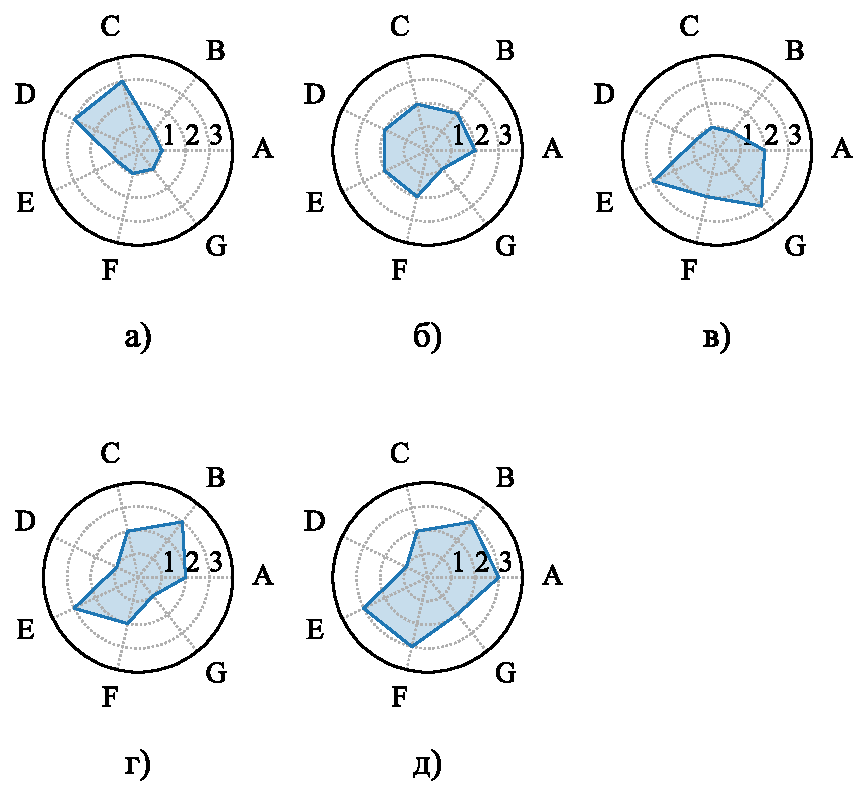
\includegraphics{part4/morphological_analyse.pdf}
	}
	\caption{Лепестковые диаграммы каждого варианта}\label{fig:morphological_analysis}
\end{figure}

Для выбора оптимального метода необходимо учитывать важность
каждого параметра в контексте нашей конкретной задачи.
Учитывая специфику многокритериальной оптимизации алгоритмов
управления электропневматическими приводами с дискретными
распределителями, были присвоены следующие веса параметрам:

\begin{itemize}
	\item A: 0.25 -- высокая важность из-за нелинейности системы;
	\item B: 0.20 -- важно для работы с множеством параметров;
	\item C: 0.15 -- важно для итеративного процесса оптимизации;
	\item D: 0.05 -- менее важно для данной задачи;
	\item E: 0.20 -- важно для работы с новыми комбинациями параметров;
	\item F: 0.10 -- важно для работы с различными типами параметров;
	\item G: 0.05 -- менее важно для данной задачи.
\end{itemize}

Используя эти веса, была вычислена взвешенная сумма для каждого метода. Рассмотрим пример расчета взвешенной суммы для метода нейронных сетей:

\begin{equation}
	\begin{split}
		S_{НС} = & 0.25 \cdot 3 + 0.20 \cdot 3 + 0.15 \cdot 2 + 0.05 \cdot 1 + \\
		+        & 0.20 \cdot 3 + 0.10 \cdot 3 + 0.05 \cdot 2 =                \\
		=        & 0.75 + 0.60 + 0.30 + 0.05 + 0.60 + 0.30 + 0.10 =            \\
		=        & 2.60
	\end{split}
\end{equation}
где $S_{НС}$ -- взвешенная сумма для нейронных сетей, а числовые значения
соответствуют оценкам из таблицы \ref{tab:method_evaluation}.

Аналогичным образом были рассчитаны взвешенные суммы для остальных методов.
Результаты представлены в таблице \ref{tab:weighted_scores}.

\begin{table}[h]
	\centering
	\caption{Взвешенные оценки методов}
	\begin{tabular}{lc}
		\midrule
		Метод                             & Взвешенная сумма \\
		\midrule
		Полиномиальная регрессия          & 1.60             \\
		Радиальные базисные функции (RBF) & 1.95             \\
		Кригинг (Гауссовы процессы)       & 1.90             \\
		Метод опорных векторов (SVM)      & 2.25             \\
		Нейронные сети                    & 2.60             \\
		\hline
	\end{tabular}
	\label{tab:weighted_scores}
\end{table}

Как видно из результатов, нейронные сети получили наивысшую взвешенную оценку
(2.60). Это объясняется тем, что они имеют высокие оценки по наиболее важным
критериям: способности к аппроксимации нелинейных зависимостей (вес 0.25),
масштабируемости (вес 0.20) и способности к обобщению (вес 0.20). Несмотря на
относительно низкую оценку по интерпретируемости результатов (1 с весом 0.05),
это не оказало значительного влияния на общий результат из-за низкого веса этого
критерия для нашей задачи.

На основе проведенного морфологического анализа с использованием метода
Цвикки, наиболее подходящим методом для построения суррогатной модели
в контексте многокритериальной оптимизации алгоритмов управления
электропневматическими приводами с дискретными распределителями
являются нейронные сети. Они получили наивысшую взвешенную оценку
благодаря своим сильным сторонам: высокой способности к аппроксимации
сложных нелинейных зависимостей, хорошей масштабируемости и работе с
высокоразмерными данными, высокой способности к обобщению и высокой
адаптивности к различным типам данных.

Несмотря на некоторые недостатки, такие как относительно низкая интерпретируемость
результатов и средняя вычислительная эффективность,
преимущества нейронных сетей в контексте данной задачи перевешивают
их недостатки. Для минимизации этих недостатков могут быть применены методы
регуляризации, техники визуализации и интерпретации нейронных сетей, а
также оптимизация архитектуры сети для повышения вычислительной эффективности.
\chapter{ПЕРЕЧЕНЬ СТЕНДОВОГО ОБОРУДОВАНИЯ}\label{app:equipment_list}
В данном приложении представлен перечень основного оборудования, использованного при
создании экспериментального стенда для исследования позиционного пневмопривода с дискретным управлением.

\begingroup
\centering
\small
\captionsetup[table]{skip=7pt} % смещение положения подписи
\begin{longtable}[c]{|m{0.2\textwidth}|m{0.3\textwidth}|m{0.25\textwidth}|}
	\caption{Перечень оборудования экспериментального стенда}\label{tab:equipment_list}
	\\[-0.45\onelineskip]
	\hline
	\textbf{Наименование}                                    & \textbf{Основные характеристики} & \textbf{Внешний вид} \\
	\hline
	\endfirsthead

	\caption*{Продолжение таблицы~\thetable}                                                                           \\[-0.45\onelineskip]
	\hline
	\textbf{Наименование}                                    & \textbf{Основные характеристики} & \textbf{Внешний вид} \\
	\hline
	\endhead
	\hline
	\endfoot
	\hline
	\endlastfoot
	Пневмоцилиндр DSNU-32-350-PPV-A                          &
	Диаметр поршня: 32 мм;
	Ход: 350 мм;
	Диаметр штока: 12 мм;
	Макс. рабочее давление: \num{1.0} МПа;
	Макс. скорость: \num{1.5} м/с.
	                                                         &
	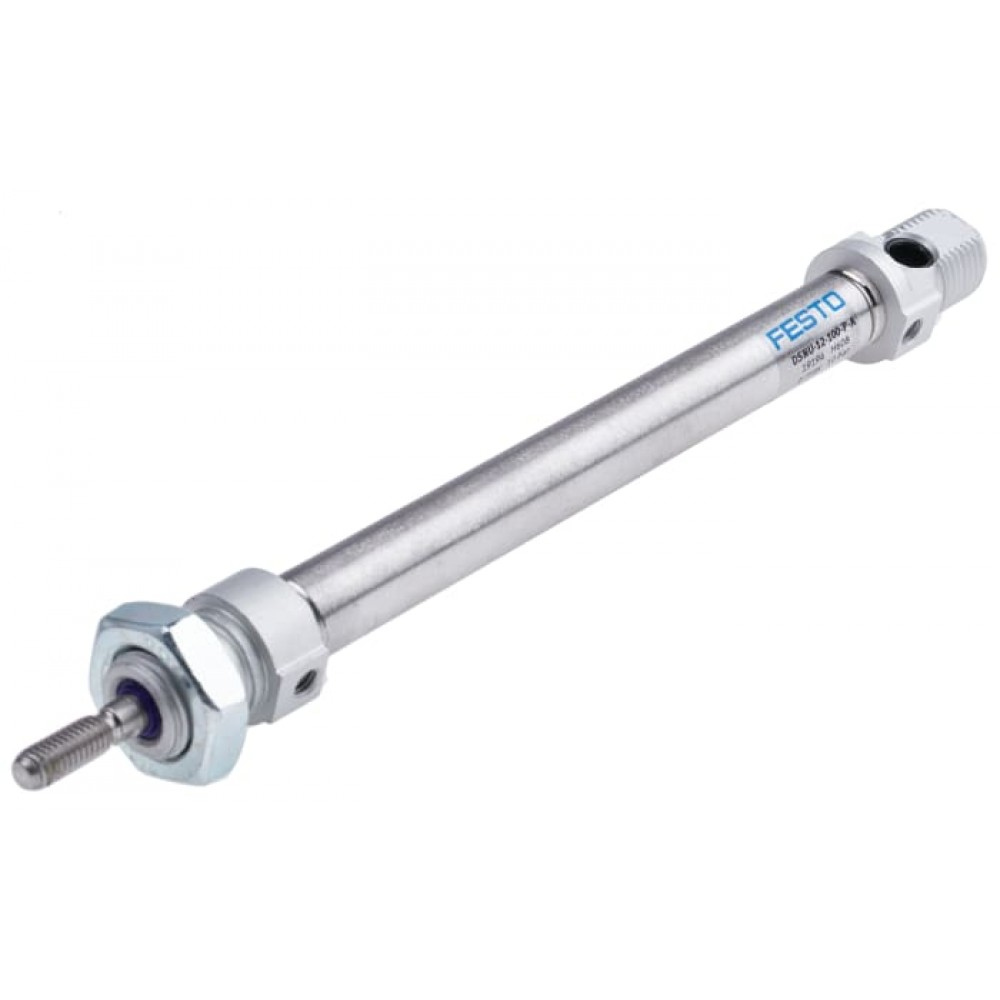
\includegraphics[width=4cm]{appendix/cylinder.jpg}                                                                 \\
	\hline
	Распределитель Camozzi AA31-0C2                          &
	Тип: 3/2 NC;
	Пропускная способность: 750 Нл/мин;
	Время переключения: 20 мс;
	Рабочее напряжение: 24В DC;
	Потребляемая мощность: \num{1.8} Вт.
	                                                         &
	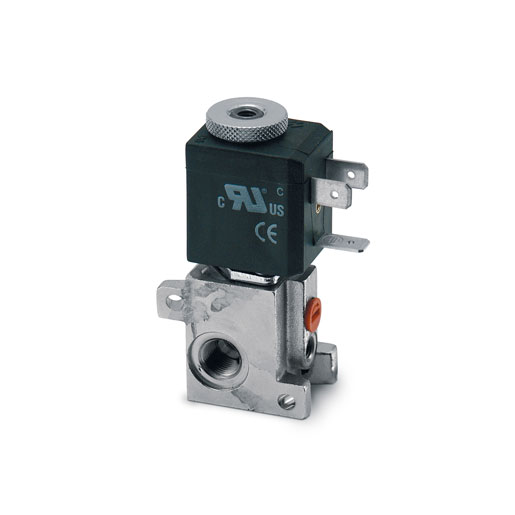
\includegraphics[width=4cm]{appendix/AA31-0C2+.jpg}                                                                \\
	\hline
	Датчик давления Festo SPAU-P10R-H-G18FD-L-PNLK-PNVBA-M8U &
	Диапазон измерения: 0–10 бар;
	Выход: аналоговый сигнал;
	Точность: $\pm \num{0.5}$\% FS;
	Рабочее напряжение: 24В DC.
	                                                         &
	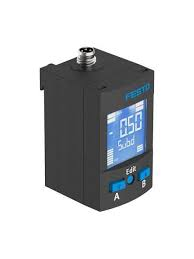
\includegraphics[width=4cm]{appendix/spau_pressure_sensor.jpg}                                                     \\
	\hline
	Датчик положения Festo MLO-POT-450-TLF                   &
	Тип: потенциометр;
	Диапазон измерения: 0~--~450 мм;
	Рабочее напряжение: 10В DC.
	                                                         &
	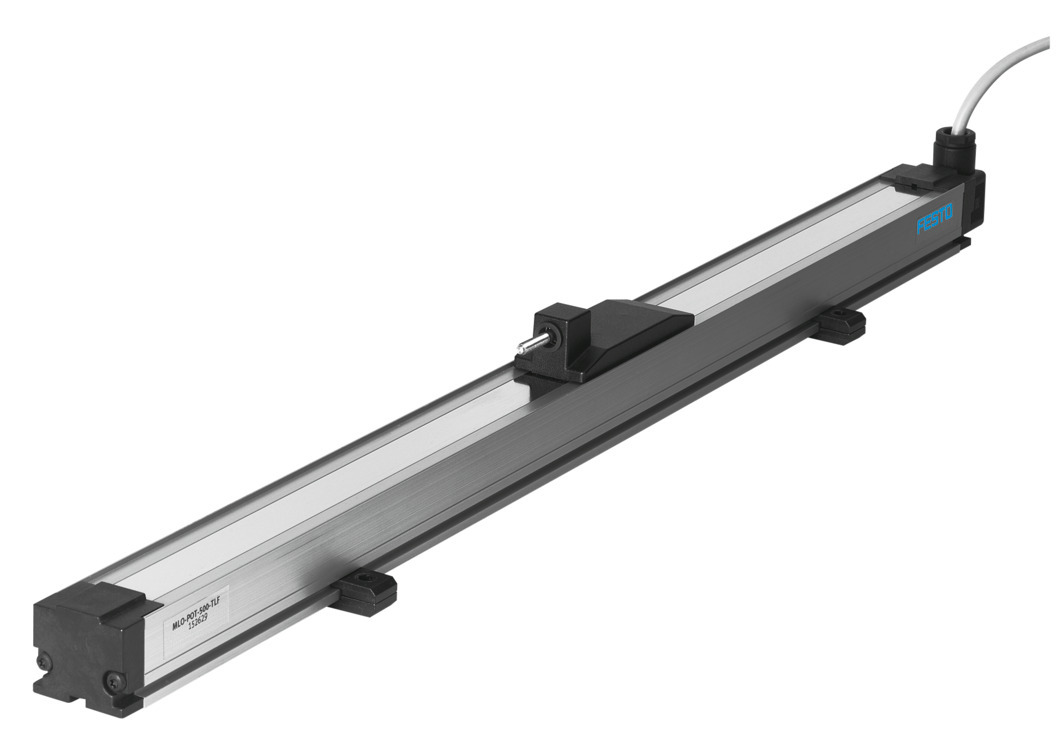
\includegraphics[width=4cm]{appendix/festo_position_sensor.jpg}                                                    \\
	\hline
	STM32F767ZI                                              &
	Микроконтроллер ARM Cortex-M7;
	Тактовая частота: 216 МГц;
	Флеш-память: 2 МБ;
	SRAM: 512 КБ;
	Набор периферии: USB, Ethernet, CAN, ADC.
	                                                         &
	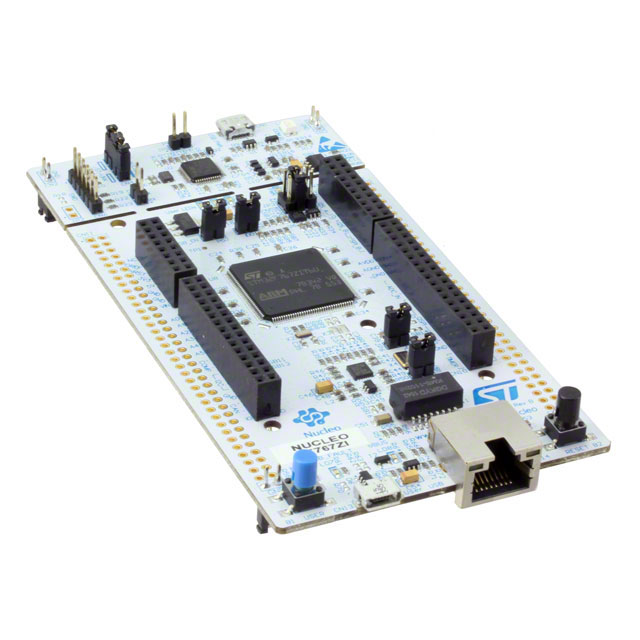
\includegraphics[width=4cm]{appendix/stm32f767zi.jpg}                                                              \\
	\hline
	Raspberry Pi 5                                           &
	Процессор: Broadcom (до \num{1.8} ГГц);
	Оперативная память: 4/8 ГБ;
	Интерфейсы: USB \num{3.0}, Gigabit Ethernet, WiFi, Bluetooth;
	Поддержка 4K видео.
	                                                         &
	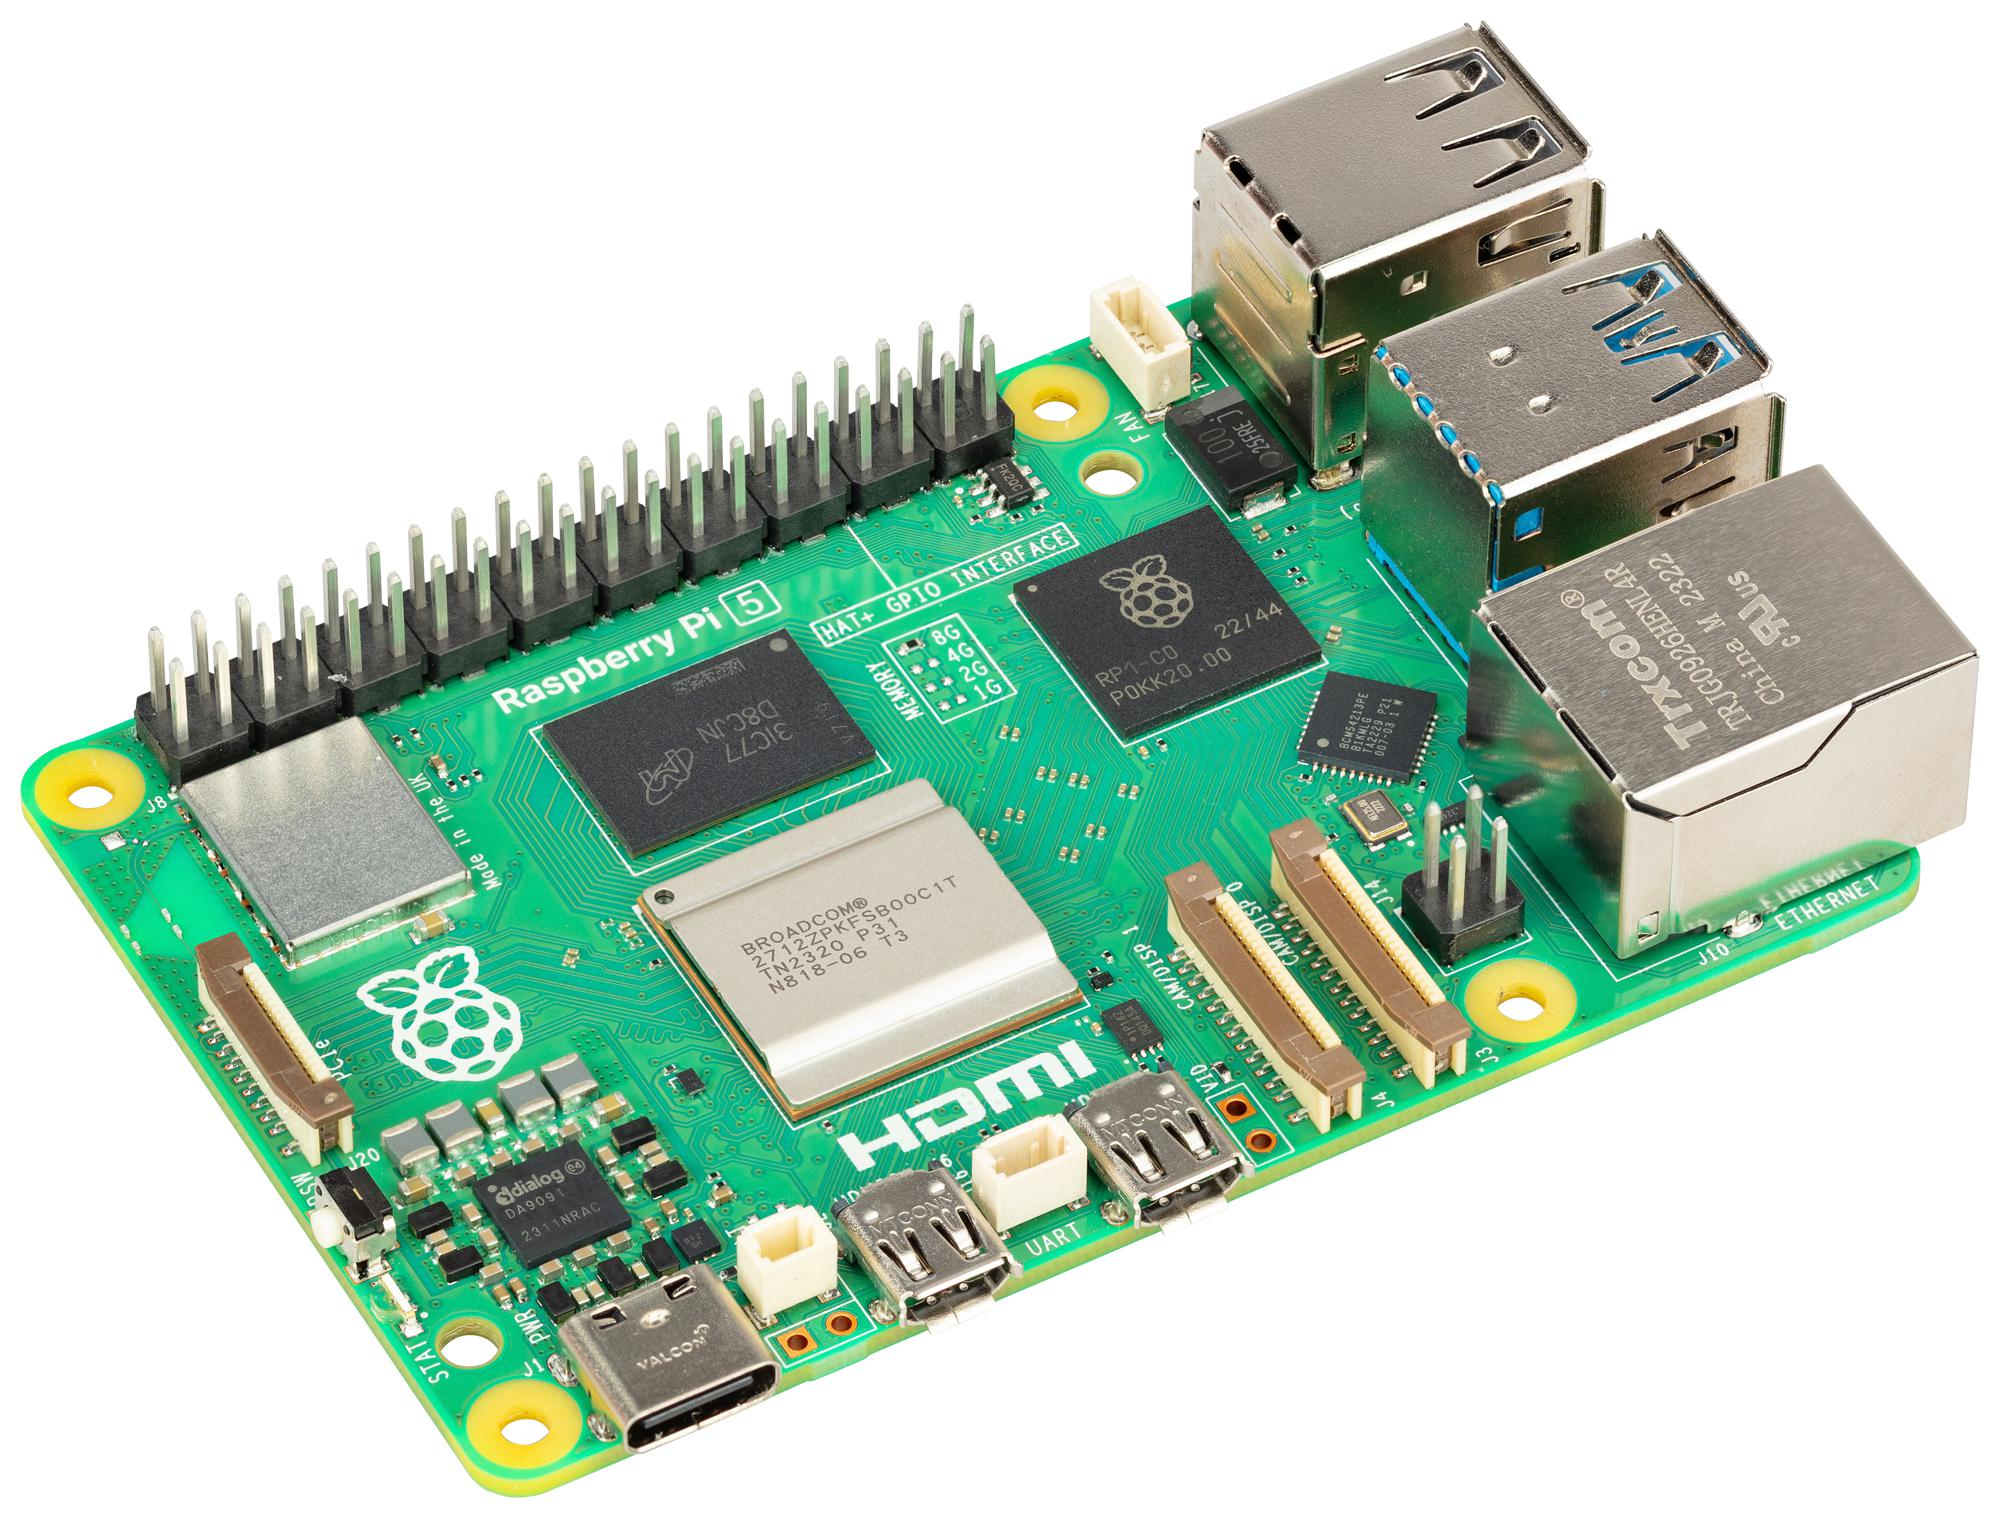
\includegraphics[width=4cm]{appendix/raspberrypi5.jpg}                                                             \\
	\hline
	АЦП ADS1256                                              &
	Разрешение: 24 бит;
	Скорость выборки: до 30 кГц;
	Интерфейс: SPI;
	Много канальный.
	                                                         &
	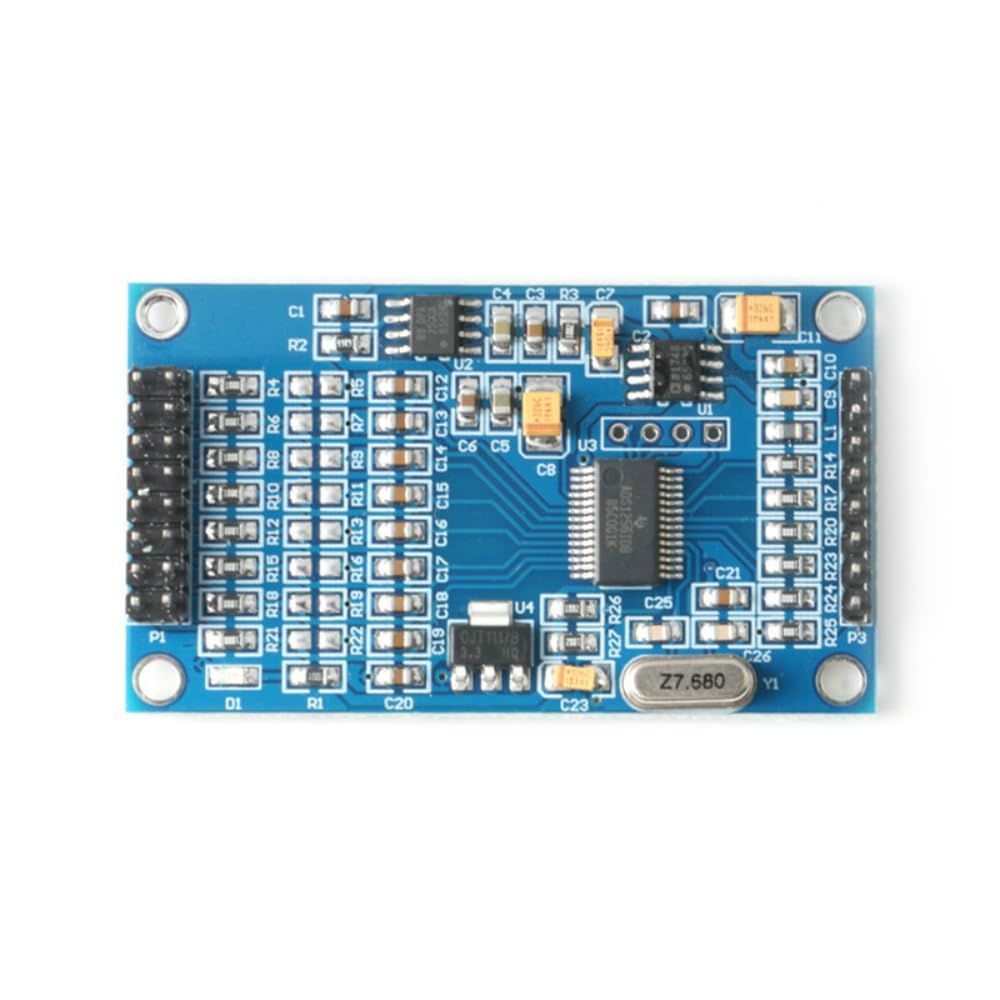
\includegraphics[width=4cm]{appendix/ads1256.jpg}                                                                  \\
	\hline
\end{longtable}
\normalsize% возвращаем шрифт к нормальному
\endgroup
\chapter{АЛГОРИТМ МЕТОДИКИ СТРУКТУРНО-ПАРАМЕТРИЧЕСКОГО СИНТЕЗА}\label{app:methodology}


\section*{Введение}

Методика структурно-параметрического синтеза позиционного пневмопривода с дискретными распределителями
представляет собой комплексный подход к определению оптимальной структуры и параметров системы управления. Данная методика
позволяет найти рациональное решение, учитывающее конфликтующие критерии: точность позиционирования, качество переходных
процессов и интенсивность переключений распределителей.

На начальном этапе структурного синтеза формируются Парето-фронты для различных управляющих
структур, что позволяет выявить взаимосвязи между критериями оптимизации и определить предпочтительные области
применения каждой из структур. На основе полученных данных создается карта предпочтительных областей применения,
которая позволяет выбрать конкурсные структуры для дальнейшего параметрического синтеза в зависимости
от требований к системе.

Последующий параметрический синтез заключается в определении оптимальных значений параметров выбранной управляющей
структуры на основе заданных требований к критериям оптимизации. Это достигается путем решения обратной
задачи с использованием построенных Парето-фронтов.

Ниже представлено детальное описание алгоритма методики структурно-параметрического
синтеза позиционного пневмопривода с дискретными распределителями.


\section*{Алгоритм построения фронтов Парето}

Построение фронтов Парето для различных управляющих структур пневмопривода направлено на
выявление взаимосвязей между показателями оптимизации и формирование базы для структурного синтеза.

\textbf{Входные данные алгоритма:}
\begin{itemize}
    \item Управляющая структура пневмопривода $S$.
    \item Множество варьируемых параметров $\mathbf{P}$.
    \item Диапазоны варьирования параметров $[\mathbf{P}_{\min}, \mathbf{P}_{\max}]$.
    \item Математическая модель пневмопривода $M$.
    \item Критерии оптимизации $\mathbf{J} = \{AC, ITAE, SI\}$.
    \item Требования к точности суррогатной модели $\varepsilon_{surr}$.
\end{itemize}

\textbf{Выходные данные алгоритма:} фронт Парето $\mathcal{PF}_{S}$ для управляющей структуры $S$.

\textbf{Алгоритм построения фронтов Парето:}

\paragraph*{Формирование плана эксперимента.}

Определяется число экспериментов $N_{exp}$ по формуле:
\begin{equation}
    N_{exp} = 10 \cdot \dim(\mathbf{P})
\end{equation}
где $\dim(\mathbf{P})$ -- размерность вектора варьируемых параметров.

Формируется план эксперимента $X = \{x_1, x_2, \ldots, x_{N_{exp}}\}$ с использованием метода латинского
гиперкуба (Latin Hypercube Sampling), обеспечивающего равномерное покрытие пространства параметров при минимальном числе экспериментов.

\paragraph*{Проведение численного моделирования.}

Для каждого набора параметров $x_i$ из плана эксперимента выполняются следующие действия:
\begin{enumerate}
    \item Установка параметров структуры управления $\mathbf{p} = x_i$.
    \item Проведение численного моделирования с использованием модели $M$ и параметров $\mathbf{p}$.
    \item Расчет значений критериев оптимизации $\mathbf{j} = \{AC, ITAE, SI\}$.
    \item Сохранение результата в массив $Y$.
\end{enumerate}

В результате формируется массив пар «параметры-критерии» $D = \{(x_i, Y_i)\}_{i=1}^{N_{exp}}$,
являющийся основой для построения суррогатной модели.

\paragraph*{Построение суррогатной модели.}

На основе собранных данных строится суррогатная модель $SM$, аппроксимирующая зависимость критериев
оптимизации от параметров управляющей структуры. В качестве суррогатной модели
используются искусственные нейронные сети с архитектурой глубокого обучения.

Процесс построения модели включает следующие подэтапы:
\begin{enumerate}
    \item Нормализация входных и выходных данных.
    \item Разделение данных на обучающую и валидационную выборки.
    \item Подбор гиперпараметров модели с использованием байесовской оптимизации.
    \item Обучение модели на обучающей выборке.
\end{enumerate}

\paragraph*{Проверка адекватности суррогатной модели.}

Для оценки качества построенной суррогатной модели используется метод
кросс-валидации. Вычисляется среднеквадратичная ошибка на тестовой выборке:
\begin{equation}
    RMSE = \sqrt{\frac{1}{N_{test}} \sum_{i=1}^{N_{test}} \| SM(x_i) - Y_i \|_2^2}.
\end{equation}

Если $RMSE > \varepsilon_{surr}$, то выполняются следующие действия:
\begin{enumerate}
    \item Увеличение размера обучающей выборки путем дополнительных экспериментов.
    \item Корректировка структуры модели (числа слоев, нейронов и т.д.).
    \item Возврат к этапу построения суррогатной модели.
\end{enumerate}

\paragraph*{Многокритериальная оптимизация.}

Для поиска Парето-оптимальных решений используется алгоритм NSGA-III (Non-dominated Sorting Genetic Algorithm).
Процесс оптимизации включает следующие этапы:
\begin{enumerate}
    \item Инициализация популяции: $\mathcal{P} = \{p_1, p_2, \ldots, p_{N_{pop}}\}.$
    \item На протяжении $N_{gen}$ поколений:
          \begin{enumerate}
              \item Оценка целевых функций для каждой особи с использованием суррогатной модели $SM$: $\mathbf{J}(p_i).$
              \item Выполнение недоминируемой сортировки популяции.
              \item Расчет краудинг-дистанций для сохранения разнообразия решений.
              \item Отбор лучших решений для следующего поколения.
              \item Применение операторов скрещивания и мутации для создания новых решений.
          \end{enumerate}
\end{enumerate}

\paragraph*{Формирование фронта Парето.}

Из последнего поколения эволюционного алгоритма выбираются
недоминируемые решения, формирующие фронт Парето:
\begin{equation}
    \mathcal{PF}_{S} = \{p \in \mathcal{P} \mid p \text{ недоминируемо}\}
\end{equation}

Дополнительно выполняются следующие операции:
\begin{enumerate}
    \item Верификация полученных решений на полной модели $M$ для исключения возможных ошибок суррогатной модели.
    \item Упорядочение решений для обеспечения гладкости фронта.
    \item Удаление дубликатов и близко расположенных решений.
\end{enumerate}

В результате выполнения данного алгоритма для каждой исследуемой управляющей
структуры пневмопривода формируется соответствующий фронт Парето, отражающий
компромисс между критериями оптимизации $AC$ (точность позиционирования), $ITAE$
(интегральный критерий качества) и $SI$ (интенсивность переключений).

\section*{Алгоритм решения обратной задачи оптимизации}

Алгоритм решения обратной задачи оптимизации направлен на определение
оптимальных параметров выбранной управляющей структуры на основе
заданных требований к критериям оптимизации.

\textbf{Входные данные алгоритма:}
\begin{itemize}
    \item Множество фронтов Парето $\{\mathcal{PF}_{S_1}, \mathcal{PF}_{S_2}, \ldots, \mathcal{PF}_{S_n}\}$ для различных управляющих структур.
    \item Целевые значения критериев $\mathbf{J}_{target} = \{AC_{target}, ITAE_{target}, SI_{target}\}$.
    \item Весовые коэффициенты $\mathbf{w} = \{w_{AC}, w_{ITAE}, w_{SI}\}$, отражающие приоритеты критериев.
\end{itemize}

\textbf{Выходные данные алгоритма:} оптимальная управляющая структура $S^*$ и вектор оптимальных параметров $\mathbf{p}^*$.

\textbf{Алгоритм решения обратной задачи оптимизации:}

\paragraph*{Нормализация критериев.}

Для обеспечения сопоставимости критериев с различной
физической природой и масштабами выполняется их нормализация:

\begin{enumerate}
    \item Для каждого фронта Парето $\mathcal{PF}_{S_i}$ определяются минимальные и максимальные значения критериев:
          \begin{equation*}
              AC_{min}^i, AC_{max}^i, ITAE_{min}^i, ITAE_{max}^i, SI_{min}^i, SI_{max}^i.
          \end{equation*}

    \item Вычисляются глобальные минимумы и максимумы по всем фронтам:
          \begin{equation*}
              \begin{aligned}
                  AC_{min}   & = \min_i AC_{min}^i,   & AC_{max}   & = \max_i AC_{max}^i ,  \\
                  ITAE_{min} & = \min_i ITAE_{min}^i, & ITAE_{max} & = \max_i ITAE_{max}^i ,\\
                  SI_{min}   & = \min_i SI_{min}^i,   & SI_{max}   & = \max_i SI_{max}^i.
              \end{aligned}
          \end{equation*}

    \item Нормализуются целевые значения критериев:
          \begin{equation*}
              \begin{aligned}
                  AC_{target}^{norm}   & = \frac{AC_{target} - AC_{min}}{AC_{max} - AC_{min}}         \\
                  ITAE_{target}^{norm} & = \frac{ITAE_{target} - ITAE_{min}}{ITAE_{max} - ITAE_{min}} \\
                  SI_{target}^{norm}   & = \frac{SI_{target} - SI_{min}}{SI_{max} - SI_{min}}
              \end{aligned}
          \end{equation*}
\end{enumerate}

\paragraph*{Поиск ближайшей точки на каждом фронте Парето.}

Для каждого фронта Парето $\mathcal{PF}_{S_i}$ выполняются следующие действия:

\begin{enumerate}
    \item Инициализация минимального расстояния $d_{min}^i = \infty$
    \item Инициализация оптимальных параметров $\mathbf{p}_{opt}^i = \emptyset$ и значений критериев $\mathbf{J}_{opt}^i = \emptyset$

    \item Для каждой точки $p \in \mathcal{PF}_{S_i}$ с соответствующими значениями критериев $\mathbf{J}_p = \{AC_p, ITAE_p, SI_p\}$:
          \begin{enumerate}
              \item Нормализация значений критериев:
                    \begin{equation*}
                        \begin{aligned}
                            AC_p^{norm}   & = \frac{AC_p - AC_{min}}{AC_{max} - AC_{min}}     ,    \\
                            ITAE_p^{norm} & = \frac{ITAE_p - ITAE_{min}}{ITAE_{max} - ITAE_{min}} ,\\
                            SI_p^{norm}   & = \frac{SI_p - SI_{min}}{SI_{max} - SI_{min}}.
                        \end{aligned}
                    \end{equation*}

              \item Вычисление взвешенного расстояния:
                    \begin{equation*}
                        d = \sqrt{
                            \begin{aligned}
                                  & w_{AC} \cdot (AC_p^{norm} - AC_{target}^{norm})^2 +       \\
                                + & w_{ITAE} \cdot (ITAE_p^{norm} - ITAE_{target}^{norm})^2 + \\
                                + & w_{SI} \cdot (SI_p^{norm} - SI_{target}^{norm})^2.
                            \end{aligned}
                        }
                    \end{equation*}

              \item Если $d < d_{min}^i$, то:
                    \begin{equation*}
                        \begin{aligned}
                            d_{min}^i          & = d                                  ,         \\
                            \mathbf{p}_{opt}^i & = \text{параметры, соответствующие точке $p$}, \\
                            \mathbf{J}_{opt}^i & = \mathbf{J}_p.
                        \end{aligned}
                    \end{equation*}
          \end{enumerate}

    \item Сохранение результата: $distances = distances \cup \{(S_i, d_{min}^i, \mathbf{p}_{opt}^i, \mathbf{J}_{opt}^i)\}.$
\end{enumerate}

\paragraph*{Выбор оптимальной структуры.}

На основе полученных расстояний определяется оптимальная управляющая структура:

\begin{enumerate}
    \item Сортировка массива $distances$ по возрастанию $d_{min}^i$
    \item Выбор структуры $S^*$ с минимальным расстоянием:
          \begin{equation}
              S^* = \arg\min_{S_i} d_{min}^i
          \end{equation}
    \item Определение оптимальных параметров $\mathbf{p}^*$ для структуры $S^*$
\end{enumerate}

\section*{Практическое применение методики}

Предложенная методика структурно-параметрического синтеза позиционного
пневмопривода с дискретными распределителями имеет следующие практические преимущества:

\begin{enumerate}
    \item Позволяет выявить предельные возможности различных структур
	управления по критериям точности позиционирования, качества
	переходных процессов и интенсивности переключений распределителей.
    
    \item Дает возможность сформировать карту предпочтительных областей
	применения различных структур управления, что существенно упрощает
	процесс выбора оптимальной структуры на этапе предварительного проектирования.
    
    \item Обеспечивает нахождение оптимальных параметров выбранной структуры
	управления на основе заданных требований к системе без необходимости
	проведения дополнительных экспериментов.
    
    \item Сокращает время проектирования за счет использования суррогатных
	моделей, позволяющих быстро оценивать эффективность различных вариантов
	структур и параметров.
    
    \item Дает возможность учитывать конфликтующие требования к системе
	и находить компромиссные решения, удовлетворяющие конкретным
	практическим задачам.
\end{enumerate}

Применение данной методики при проектировании позиционных пневмоприводов с
дискретными распределителями позволяет достичь оптимального соотношения между
точностью позиционирования, быстродействием и ресурсом системы в соответствии
с требованиями конкретного технологического процесса без необходимости проведения
трудоемких экспериментальных исследований.

% \section*{Алгоритм построения фронтов Парето (этап 1)}

% Первый этап методики заключается в построении фронтов Парето для различных управляющих структур пневмопривода с целью выявления взаимосвязей между критериями оптимизации. Алгоритм данного этапа представлен ниже.

% Входными данными алгоритма являются:
% \begin{itemize}
% 	\item Управляющая структура пневмопривода $S$
% 	\item Множество варьируемых параметров $\mathbf{P}$
% 	\item Диапазоны варьирования параметров $[\mathbf{P}_{\min}, \mathbf{P}_{\max}]$
% 	\item Математическая модель пневмопривода $M$
% 	\item Критерии оптимизации $\mathbf{J} = \{AC, ITAE, SI\}$
% 	\item Требования к точности суррогатной модели $\varepsilon_{surr}$
% \end{itemize}

% Выходными данными алгоритма является фронт Парето $\mathcal{PF}_{S}$ для управляющей структуры $S$.

% \textbf{Алгоритм построения фронтов Парето состоит из следующих шагов:}

% \textbf{Шаг 1. Формирование плана эксперимента.}
% \vspace{0.5em}

% Определяется число экспериментов $N_{exp}$ по формуле:
% \begin{equation}
% 	N_{exp} = 10 \cdot \dim(\mathbf{P})
% \end{equation}
% где $\dim(\mathbf{P})$ -- размерность вектора варьируемых параметров.

% Формируется план эксперимента $X = \{x_1, x_2, \ldots, x_{N_{exp}}\}$ с использованием метода латинского гиперкуба (Latin Hypercube Sampling), обеспечивающего равномерное покрытие пространства параметров при минимальном числе экспериментов.

% \textbf{Шаг 2. Проведение численного моделирования.}
% \vspace{0.5em}

% Для каждого набора параметров $x_i$ из плана эксперимента выполняются следующие действия:
% \begin{enumerate}
% 	\item Установка параметров структуры управления $\mathbf{p} = x_i$
% 	\item Проведение численного моделирования с использованием модели $M$ и параметров $\mathbf{p}$
% 	\item Расчет значений критериев оптимизации $\mathbf{j} = \{AC, ITAE, SI\}$
% 	\item Сохранение результата в массив $Y$
% \end{enumerate}

% В результате формируется массив пар «параметры-критерии» $D = \{(x_i, Y_i)\}_{i=1}^{N_{exp}}$, являющийся основой для построения суррогатной модели.

% \textbf{Шаг 3. Построение суррогатной модели.}
% \vspace{0.5em}

% На основе собранных данных строится суррогатная модель $SM$, аппроксимирующая зависимость критериев оптимизации от параметров управляющей структуры. В качестве суррогатной модели могут использоваться:
% \begin{itemize}
% 	\item Искусственные нейронные сети с архитектурой глубокого обучения
% 	\item Модели на основе гауссовских процессов
% 	\item Ансамбли регрессионных деревьев
% \end{itemize}

% Процесс построения модели включает следующие подэтапы:
% \begin{enumerate}
% 	\item Нормализация входных и выходных данных
% 	\item Разделение данных на обучающую и валидационную выборки
% 	\item Подбор гиперпараметров модели с использованием байесовской оптимизации
% 	\item Обучение модели на обучающей выборке
% \end{enumerate}

% \textbf{Шаг 4. Проверка адекватности суррогатной модели.}
% \vspace{0.5em}

% Для оценки качества построенной суррогатной модели используется метод кросс-валидации. Вычисляется среднеквадратичная ошибка на тестовой выборке:
% \begin{equation}
% 	RMSE = \sqrt{\frac{1}{N_{test}} \sum_{i=1}^{N_{test}} \| SM(x_i) - Y_i \|_2^2}
% \end{equation}

% Если $RMSE > \varepsilon_{surr}$, то выполняются следующие действия:
% \begin{enumerate}
% 	\item Увеличение размера обучающей выборки путем дополнительных экспериментов
% 	\item Корректировка структуры модели (числа слоев, нейронов и т.д.)
% 	\item Возврат к шагу 3
% \end{enumerate}

% \textbf{Шаг 5. Многокритериальная оптимизация.}
% \vspace{0.5em}

% Для поиска Парето-оптимальных решений используется алгоритм NSGA-II или NSGA-III (Non-dominated Sorting Genetic Algorithm). Процесс оптимизации включает следующие этапы:
% \begin{enumerate}
% 	\item Инициализация популяции: $\mathcal{P} = \{p_1, p_2, \ldots, p_{N_{pop}}\}$
% 	\item На протяжении $N_{gen}$ поколений:
% 	      \begin{enumerate}
% 		      \item Оценка целевых функций для каждой особи с использованием суррогатной модели $SM$: $\mathbf{J}(p_i)$
% 		      \item Выполнение недоминируемой сортировки популяции
% 		      \item Расчет краудинг-дистанций для сохранения разнообразия решений
% 		      \item Отбор лучших решений для следующего поколения
% 		      \item Применение операторов скрещивания и мутации для создания новых решений
% 	      \end{enumerate}
% \end{enumerate}

% \textbf{Шаг 6. Формирование фронта Парето.}
% \vspace{0.5em}

% Из последнего поколения эволюционного алгоритма выбираются недоминируемые решения, формирующие фронт Парето:
% \begin{equation}
% 	\mathcal{PF}_{S} = \{p \in \mathcal{P} \mid p \text{ недоминируемо}\}
% \end{equation}

% Дополнительно выполняются следующие операции:
% \begin{enumerate}
% 	\item Верификация полученных решений на полной модели $M$ для исключения возможных ошибок суррогатной модели
% 	\item Упорядочение решений для обеспечения гладкости фронта
% 	\item Удаление дубликатов и близко расположенных решений
% \end{enumerate}

% В результате выполнения данного алгоритма для каждой исследуемой управляющей структуры пневмопривода формируется соответствующий фронт Парето,
% отражающий компромисс между критериями оптимизации $AC$ (точность позиционирования),
% $ITAE$ (интегральный критерий качества) и $SI$ (интенсивность переключений).

% \section*{Алгоритм решения обратной задачи оптимизации (этап 2)}

% Второй этап методики предполагает решение обратной задачи оптимизации, заключающейся в определении оптимальных параметров выбранной управляющей структуры на основе заданных требований к критериям оптимизации.

% Входными данными алгоритма являются:
% \begin{itemize}
% 	\item Множество фронтов Парето $\{\mathcal{PF}_{S_1}, \mathcal{PF}_{S_2}, \ldots, \mathcal{PF}_{S_n}\}$ для различных управляющих структур
% 	\item Целевые значения критериев $\mathbf{J}_{target} = \{AC_{target}, ITAE_{target}, SI_{target}\}$
% 	\item Весовые коэффициенты $\mathbf{w} = \{w_{AC}, w_{ITAE}, w_{SI}\}$, отражающие приоритеты критериев
% \end{itemize}

% Выходными данными алгоритма являются оптимальная управляющая структура $S^*$ и вектор оптимальных параметров $\mathbf{p}^*$.

% \textbf{Алгоритм решения обратной задачи оптимизации состоит из следующих шагов:}

% \textbf{Шаг 1. Нормализация критериев.}
% \vspace{0.5em}

% Для обеспечения сопоставимости критериев с различной физической природой и масштабами выполняется их нормализация:

% \begin{enumerate}
% 	\item Для каждого фронта Парето $\mathcal{PF}_{S_i}$ определяются минимальные и максимальные значения критериев:
% 	      \begin{equation*}
% 		      AC_{min}^i, AC_{max}^i, ITAE_{min}^i, ITAE_{max}^i, SI_{min}^i, SI_{max}^i
% 	      \end{equation*}

% 	\item Вычисляются глобальные минимумы и максимумы по всем фронтам:
% 	      \begin{equation*}
% 		      \begin{aligned}
% 			      AC_{min}   & = \min_i AC_{min}^i,   & AC_{max}   & = \max_i AC_{max}^i   \\
% 			      ITAE_{min} & = \min_i ITAE_{min}^i, & ITAE_{max} & = \max_i ITAE_{max}^i \\
% 			      SI_{min}   & = \min_i SI_{min}^i,   & SI_{max}   & = \max_i SI_{max}^i
% 		      \end{aligned}
% 	      \end{equation*}

% 	\item Нормализуются целевые значения критериев:
% 	      \begin{equation*}
% 		      \begin{aligned}
% 			      AC_{target}^{norm}   & = \frac{AC_{target} - AC_{min}}{AC_{max} - AC_{min}}         \\
% 			      ITAE_{target}^{norm} & = \frac{ITAE_{target} - ITAE_{min}}{ITAE_{max} - ITAE_{min}} \\
% 			      SI_{target}^{norm}   & = \frac{SI_{target} - SI_{min}}{SI_{max} - SI_{min}}
% 		      \end{aligned}
% 	      \end{equation*}
% \end{enumerate}

% \textbf{Шаг 2. Поиск ближайшей точки на каждом фронте Парето.}
% \vspace{0.5em}

% Для каждого фронта Парето $\mathcal{PF}_{S_i}$ выполняются следующие действия:

% \begin{enumerate}
% 	\item Инициализация минимального расстояния $d_{min}^i = \infty$
% 	\item Инициализация оптимальных параметров $\mathbf{p}_{opt}^i = \emptyset$ и значений критериев $\mathbf{J}_{opt}^i = \emptyset$

% 	\item Для каждой точки $p \in \mathcal{PF}_{S_i}$ с соответствующими значениями критериев $\mathbf{J}_p = \{AC_p, ITAE_p, SI_p\}$:
% 	      \begin{enumerate}
% 		      \item Нормализация значений критериев:
% 		            \begin{equation*}
% 			            \begin{aligned}
% 				            AC_p^{norm}   & = \frac{AC_p - AC_{min}}{AC_{max} - AC_{min}}         \\
% 				            ITAE_p^{norm} & = \frac{ITAE_p - ITAE_{min}}{ITAE_{max} - ITAE_{min}} \\
% 				            SI_p^{norm}   & = \frac{SI_p - SI_{min}}{SI_{max} - SI_{min}}
% 			            \end{aligned}
% 		            \end{equation*}

% 		      \item Вычисление взвешенного расстояния:
% 		            \begin{equation*}
% 			            d = \sqrt{
% 				            \begin{aligned}
% 					              & w_{AC} \cdot (AC_p^{norm} - AC_{target}^{norm})^2 +       \\
% 					            + & w_{ITAE} \cdot (ITAE_p^{norm} - ITAE_{target}^{norm})^2 + \\
% 					            + & w_{SI} \cdot (SI_p^{norm} - SI_{target}^{norm})^2
% 				            \end{aligned}
% 			            }
% 		            \end{equation*}

% 		      \item Если $d < d_{min}^i$, то:
% 		            \begin{equation*}
% 			            \begin{aligned}
% 				            d_{min}^i          & = d                                           \\
% 				            \mathbf{p}_{opt}^i & = \text{параметры, соответствующие точке $p$} \\
% 				            \mathbf{J}_{opt}^i & = \mathbf{J}_p
% 			            \end{aligned}
% 		            \end{equation*}
% 	      \end{enumerate}

% 	\item Сохранение результата: $distances = distances \cup \{(S_i, d_{min}^i, \mathbf{p}_{opt}^i, \mathbf{J}_{opt}^i)\}$
% \end{enumerate}

% \textbf{Шаг 3. Выбор оптимальной структуры.}
% \vspace{0.5em}

% На основе полученных расстояний определяется оптимальная управляющая структура:

% \begin{enumerate}
% 	\item Сортировка массива $distances$ по возрастанию $d_{min}^i$
% 	\item Выбор структуры $S^*$ с минимальным расстоянием:
% 	      \begin{equation}
% 		      S^* = \arg\min_{S_i} d_{min}^i
% 	      \end{equation}
% 	\item Определение оптимальных параметров $\mathbf{p}^*$ для структуры $S^*$
% \end{enumerate}

        % Приложения

\setcounter{totalappendix}{\value{chapter}} % Подсчёт количества приложений

\end{document}
